% ----------------------------------------------------------------------
%                   LATEX TEMPLATE FOR PhD THESISau
% ----------------------------------------------------------------------

% based on Harish Bhanderi's PhD/MPhil template, then Uni Cambridge
% http://www-h.eng.cam.ac.uk/help/tpl/textprocessing/ThesisStyle/
% corrected and extended in 2007 by Jakob Suckale, then MPI-CBG PhD programme
% and made available through OpenWetWare.org - the free biology wiki
% Modified to conform with University of Pennsylvania Thesis Requirements 
% by Alan Meert & David F. Moore, 2013, Dept. of Physics and Astronomy

%: --------------------------------------------------------------------------
%: Style file for Latex
%: Specify openright if printing double-sided, openany if single-sided
%: --------------------------------------------------------------------------
\documentclass[11pt, openany, oneside]{Latex/Classes/PhDthesisPSnPDF}
\usepackage{lipsum} % this just creates filler text when needed

%: --------------------------------------------------------------------------
%: Use Natbib for non-standard citations 
%: --------------------------------------------------------------------------
%: uncomment below to change from standard TeX in-text citations to
%: author-year in-text citations. Should be used together with the 
%: PhDbiblio-intext-twoauth.bst file (included with this project) or 
%: some other acceptable .bst file 
%: --------------------------------------------------------------------------

%\usepackage[authoryear]{natbib}
%  \bibpunct{(}{)}{;}{a}{}{,}

%: --------------------------------------------------------------------------
%: The end user may modify these files to personalize and define macros
%: --------------------------------------------------------------------------
\usepackage{Latex/StyleFiles/UserDefs} % Define any user-defined Macros and functions in this file.
\usepackage{Latex/StyleFiles/matt}
% This file contains macros that can be called up from connected TeX files
% It helps to summarise repeated code, e.g. figure insertion (see below).

% insert a centered figure with caption and description
% parameters 1:filename, 2:title, 3:description and label
\newcommand{\figuremacro}[3]{
	\begin{figure}[htbp]
		\centering
		\includegraphics[width=1\textwidth]{#1}
		\caption[#2]{\textbf{#2} - #3}
		\label{#1}
	\end{figure}
}

% insert a centered figure with caption and description AND WIDTH
% parameters 1:filename, 2:title, 3:description and label, 4: textwidth
% textwidth 1 means as text, 0.5 means half the width of the text
\newcommand{\figuremacroW}[4]{
	\begin{figure}[htbp]
		\centering
		\includegraphics[width=#4\textwidth]{#1}
		\caption[#2]{\textbf{#2} - #3}
		\label{#1}
	\end{figure}
}

% inserts a figure with wrapped around text; only suitable for NARROW figs
% o is for outside on a double paged document; others: l, r, i(inside)
% text and figure will each be half of the document width
% note: long captions often crash with adjacent content; take care
% in general: above 2 macro produce more reliable layout
\newcommand{\figuremacroN}[3]{
	\begin{wrapfigure}{o}{0.5\textwidth}
		\centering
		\includegraphics[width=0.48\textwidth]{#1}
		\caption[#2]{{\small\textbf{#2} - #3}}
		\label{#1}
	\end{wrapfigure}
}

% predefined commands by Harish
\newcommand{\PdfPsText}[2]{
  \ifpdf
     #1
  \else
     #2
  \fi
}

\newcommand{\IncludeGraphicsH}[3]{
  \PdfPsText{\includegraphics[height=#2]{#1}}{\includegraphics[bb = #3, height=#2]{#1}}
}

\newcommand{\IncludeGraphicsW}[3]{
  \PdfPsText{\includegraphics[width=#2]{#1}}{\includegraphics[bb = #3, width=#2]{#1}}
}

\newcommand{\InsertFig}[3]{
  \begin{figure}[!htbp]
    \begin{center}
      \leavevmode
      #1
      \caption{#2}
      \label{#3}
    \end{center}
  \end{figure}
}


 % Some prewritten Macros for Use in Latex


%: ----------------------------------------------------------------------
%:                  User information
% -----------------------------------------------------------------------

% DISSERTATION TITLE
\title{Towards Constraints on the Epoch of Reionization} %The title of your thesis
% Optional Sub-title
\SubTitle{A Phenomenological Approach} %comment if you don't want a subtitle

% PDF information
\PDFSubject{Physics}
\PDFkeywords{science, dogs, rainbows}

%YOU 
\author[mattma@sas.upenn.edu]{Matthew Malloy} %[your email address]{your name}

% Degree information
\DegreeDate{2015} % expected year of graduation.
\degree{Doctor of Philosophy}

%YOUR DEPARTMENT and UNIVERSITY
\collegeordept{\href{http://www.physics.upenn.edu}{Physics and Astronomy}}
\university{\href{http://www.upenn.edu}{University of Pennsylvania}}

%YOUR ADVISOR
\supervisor[Professor, Physics and Astronomy]{Adam Lidz}

% Your Department Graduate chair
\gradchair[Professor, Physics and Astronomy]{R.U. Stupid}

% Additional Comitee Members [title]{Name}
% Up to 6 members are allowed, comment out unusued members
% Members beyond 6 require modification of class file.
\firstcomittee[Professor, Physics and Astronomy]{Doc 1}
\secondcomittee[Professor, Physics and Astronomy]{Doc 2}
\thirdcomittee[Professor, Physics and Astronomy]{Doc 3}
\fourthcomittee[Professor, Physics and Astronomy]{Doc 4}
\fifthcomittee[Professor, Physics and Astronomy]{Doc 5}
\sixthcomittee[Professor, Physics and Astronomy]{Doc 6}


% Copyright statement of your choice
\CopyrightStatement{This work is licensed under the Creative Commons
Attribution-NonCommercial-ShareAlike 4.0 License.\newline
\noindent To view a copy of this license, visit
\href{http://creativecommons.org/licenses/by-nc-sa/4.0/}{%
http://creativecommons.org/licenses/by-nc-sa/4.0/}
}

%: --------------------------------------------------------------
%:                  BEGIN THE DOCUMENT!!!
% --------------------------------------------------------------
\begin{document}

% sets line spacing
\renewcommand\baselinestretch{1.2}
\baselineskip=18pt plus1pt

%: ------------------------------------------------------------------------
%:                  FRONT MATTER: dedications, abstract,..
% -------------------------------------------------------------------------

%: ----------------------- generate cover page ----------------------------
\maketitle  

%: ----------------------- generate copyright page ------------------------
\makecopyright  

%: ----------------------- Include a Dedication ---------------------------
% Thesis Dedictation ---------------------------------------------------

\begin{dedication} %this creates the heading for the dedication page

\large\emph{``Nobody exists on purpose, nobody belongs anywhere, everybody's gonna die. Come watch TV."}

\end{dedication}

% ----------------------------------------------------------------------

%: ----------------------- Include an Acknowledgement ---------------------
% Thesis Acknowledgements ------------------------------------------------

\begin{acknowledgements}

A huge number of people were hugely important. You will fill this in later.

\end{acknowledgements}

% ------------------------------------------------------------------------




%: ----------------------- abstract ---------------------------------------

% Thesis Abstract -----------------------------------------------------

\begin{abstracts}

350 words maximum here\ldots

\end{abstracts}

% ---------------------------------------------------------------------- 


%: ----------------------- generate Table of Contents ---------------------
\setcounter{secnumdepth}{1} % organisational level that receives a numbers
\setcounter{tocdepth}{3}    % print table of contents for level 3
\tableofcontents            % print the table of contents
% levels are: 0 - chapter, 1 - section, 2 - subsection, 3 - subsection


%: ----------------------- generate list of tables ------------------------
\listoftables  % print list of tables

%: ----------------------- generate list of figures ------------------------
\listoffigures	

%: ----------------------- Preface -----------------------------------------
% Thesis Preface -----------------------------------------------------

\begin{preface}

Perhaps you feel inclined to preface your work with poetic 
self-reflection about why you took up this project? Maybe a story 
that's kind of boring and ends with a joke that's not funny? Go for it!


\end{preface}

% ---------------------------------------------------------------------- 



%: -------------------------------------------------------------------------
%:                  MAIN DOCUMENT SECTION
% --------------------------------------------------------------------------

\mainmatter


%: ----------------------- introduction file header -----------------------


% the code below specifies where the figures are stored
\ifpdf
    \graphicspath{{introduction/figures/PNG/}{introduction/figures/PDF/}{introduction/figures/}}
\else
    \graphicspath{{introduction/figures/EPS/}{introduction/figures/}}
\fi

% ----------------------------------------------------------------------
%: ----------------------- introduction content ----------------------- 
% ----------------------------------------------------------------------
\chapter{First Things First}
\section{Cosmic Context}\label{sec:CosmicContext}

The subject of this thesis is the ``Epoch of Reionization", also known as ``hydrogen reionization" or ``reionization" or simply the ``EoR". Let us start with a brief description of what this process is, how it relates to the evolution of the Universe as a whole, and what the open problems are regarding reionization that we are trying to solve. 


The problem of reionization arises when trying to reconcile observations of the early Universe with those of the present-day Universe. Namely, Big Bang nucleosynthesis and observations of the Cosmic Microwave Background (CMB, discussed in \S \ref{sec:CMB})\gloss{CMB}{Cosmic Microwave Background. This is the earliest available snapshot of the Universe and is composed of light which has travelled from the surface of last scattering to today, largely unimpeded.} demonstrate that, when the Universe was $\sim$380,000 years old, neutral hydrogen and helium constituted the vast majority of the baryonic matter. However, observations of nearby quasars (specifically, the \lya\ forest, discussed in \S \ref{sec:LyaForest}) demonstrate that the gas between the galaxies, dubbed the intergalactic medium (IGM)\gloss{IGM}{Intergalactic medium. This refers to the gas between galaxies, which constitutes most of the baryonic matter in the Universe.}, today is almost entirely ionized.\footnote{In \S \ref{sec:LyaForest}, we discuss how the lack of \lya\ absorption in quasar spectra is suggestive of a highly-ionized IGM. However, when this was first observed in 1965 (\citealt{1965ApJ...142.1633G}), it was not obvious that this was indicative of an \textit{ionized} IGM rather than a scenario where galaxy formation was so efficient as to remove almost all of the gas from the IGM. See \cite{meiksin2009physics} for a nice review of the physics of the IGM.} Therefore, it must be the case that some very energetic process occurred in the intervening $\sim$13 billion years which stripped the electrons from almost all of the atoms in the IGM. We refer to this process as the Epoch of Reionization.


Technically, several ionizations have to take place: ionizing hydrogen, singly ionizing helium, and doubly ionizing helium with the required energies per ionization being 13.6 eV, 24.6 eV, and 54.4 eV, respectively. Since the first two processes require similar energies, they are thought to occur concurrently. However, the complete ionization of helium requires four times as much energy as for hydrogen and likely occurs significantly later and as a result of a different process (see, e.g., \S 6.3.2 of \citealt{barkana2001beginning}). For this thesis, we focus exclusively on hydrogen ionization and the single ionization of helium and treat the term ``reionization" as being synonymous with this. 


\begin{figure}[h]
  \centering
  \includegraphics[width=14cm]{BellUniverse.eps}
  \caption{Milestones in the evolution of the Universe from the Big Bang to today.(Photo from NASA WMAP science team)}
  \label{fig:NASAWMAP}
\end{figure}


To help understand where reionization fits into the evolution of the Universe as a whole, we can refer to Figure \ref{fig:NASAWMAP}, which shows the qualitative evolution of the Universe starting with the inflation and the CMB on the far left and ending with the present-day Universe on the right and spanning $\sim$13.8 billion years. One of the exciting aspects of reionization is that so little about it is known for sure. However, a reasonable round-number placement of reionization in this figure would be that it was an extended process that occurred somewhere between $\sim$500 million years after the Big Bang and 1 billion years after the Big Bang, likely coinciding with the formation of the first galaxies. 


The manner in which reionization progressed is also not known for sure and depends on the specifics of what energetic process is at its root. For example, if ``softer" sources, emitting ionizing radiation in the UV but not X-ray, drove reionization, then these photons will see a relatively high photoionization cross section and will not travel far before ionizing hydrogen in their path. Under this scenario, the state of the Universe during reionization would likely resemble a two-phase medium with ionized regions surrounding the ionizing sources and sharp boundaries between the ionized regions and the neutral IGM. Eventually, as the ionized regions grew, they would overlap until the entire IGM was ionized. This is the expected course for reionization in the event that it is driven by the first galaxies.	


If reionization is driven by sources with a ``harder" spectrum, emitting ionizing radiation strongly in X-ray, then the photoionization cross section of these photons will be relatively low. This is because, for photons with $E_{\gamma} \gg 13.6e\text{V}$, the cross section falls off as $\sigma \sim 1/\nu^3$. Because of this, ionizing radiation from these sources will travel \textit{farther} on average before ionizing a hydrogen atom. This will result in transitions between fully-ionized regions and fully-neutral regions being more gradual. This is the expected scenario in the case where reionization is driven by X-ray binaries or quasars. 


Additionally, \cite{McQuinn2007} investigate how the morphology of ionized regions depends on how massive the ionizing sources are. In Figure \ref{fig:McQuinnMorph}, \cite{McQuinn2007} show several reionization simulation outputs. Each panel shows the ionization field for a snapshot of a simulation. Black regions are neutral and white regions are ionized. In each row, the fraction of hydrogen atoms in the IGM that are neutral (dubbed the neutral fraction, denoted $\axhi$) is fixed and decreases for lower rows. Each column corresponds to a different mass distribution for the ionizing sources, with the masses essentially increasing as you move rightward (and assuming galaxies ionize the Universe). As such, the rightmost column demonstrates a plausible reionization scenario when very rare and massive sources dominate the ionizing photon budget. We can see this results in larger ionized regions for a fixed neutral fraction and sharper boundaries between the neutral and ionized regions. On the other hand, the left-hand columns correspond to a relatively larger contribution to the ionizing photon budget from less-massive sources. The result is a more homogeneous ionization with the ionized regions being smaller on average. Despite the uncertainties in the nature of reionization, Figure \ref{fig:McQuinnMorph} gives a qualitative picture of how reionization likely progressed: with ionized bubbles forming around sources, growing, and eventually overlapping until the effectively occupy the entire IGM. 


\begin{figure}[h]
  \centering
  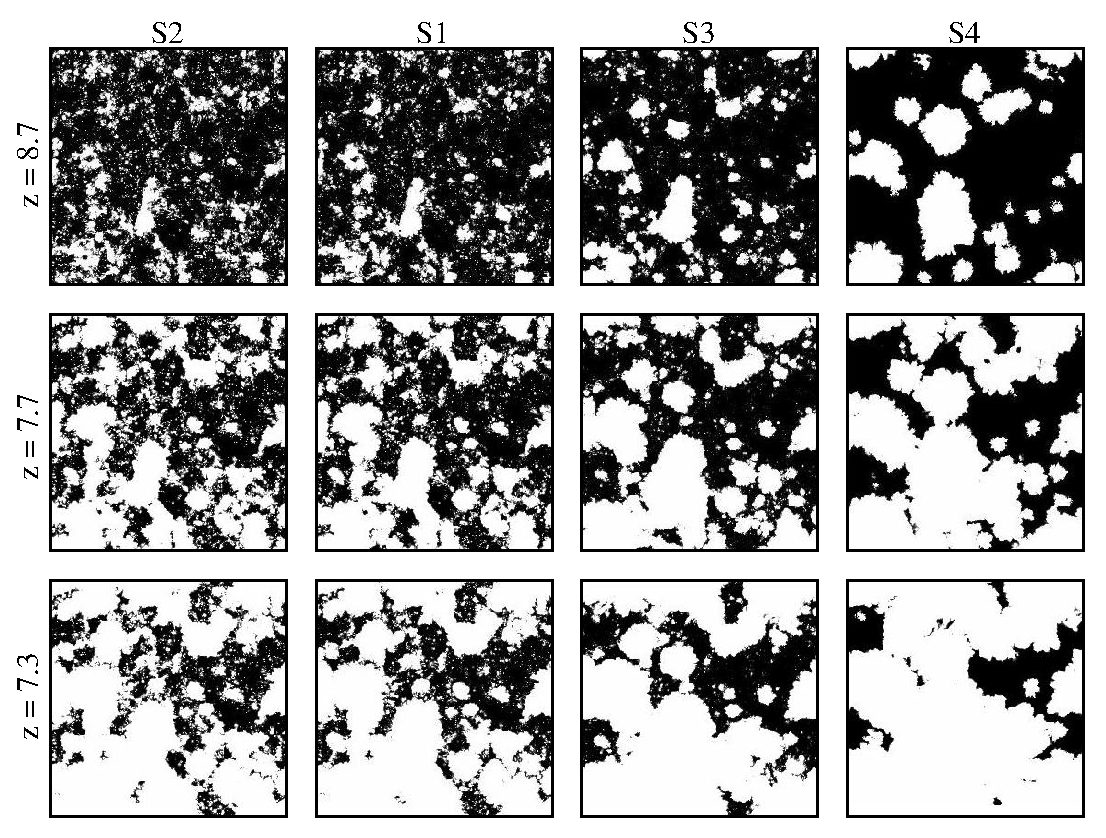
\includegraphics[width=14cm]{McQuinnHIITopology.eps}
  \caption{Simulation outputs from \cite{McQuinn2007} showing four different reionization models. Each row is at fixed $\axhi$ with $\axhi = 0.8$ (top), 0.5 (middle), 0.3 (bottom). The luminosities of the ionizing sources are related to their mass by $\dot{N} \propto m^{1/3}$ (left), $\dot{N} \propto m$ (left-middle), $\dot{N}\propto m^{5/3}$ (right-middle), and $\dot{N} \propto m$ but with a larger minimum mass (right). }
  \label{fig:McQuinnMorph}
\end{figure}


With this qualitative picture in mind, it may be worth emphasizing why astrophysicists and cosmologists care about reionization in the first place. First, the Epoch of Reionization is a significant missing piece in the story of the evolution of the Universe and represents a period in the history of the Universe where we have very few direct observations. Work towards understanding reionization is in line with the overarching goal of pushing observations further and further back in time. Second, the Epoch of Reionization marks the time when radiation from luminous sources became the dominant influence on the IGM and understanding the source of this radiation is interesting in its own right. Understanding the evolution in the properties and number of these bright sources is essential for complete cosmological models. Additionally, while the best guess for the source of the ionizing radiation is dwarf galaxies, it is possible that reionization studies will reveal more exotic and unexpected scenarios, such as annihilating dark matter playing a significant role. Third, the temperature and ionization state of the gas in the Universe plays a regulatory role in galaxy formation: hot and ionized gas will take longer to cool and collapse than cold neutral gas. Since reionization significantly affects both the temperature and ionization state of the gas, understanding reionization will be essential for understanding subsequent galaxy formation. 


Toward these goals, astrophysicists and cosmologists are striving for a thorough understanding of the timing and nature of reionization. When did it happen? How long did it take? What were the ionizing sources? What were the properties of the ionized regions and how did they evolve? These are the questions we should keep in mind throughout the rest of this thesis.

\subsection{Simulations}

In this thesis, we aim to develop measurements that can be applied to existing and future data sets in order to constrain the process of reionization.  In order to do this, we utilize simulations of the Universe at different times and assuming different cosmological and astrophysical parameters. We then process the simulation outputs according to the details of specific experiments in order to generate plausible mock observations from those experiments. While I perform this processing, the simulations used are not my own and the exact simulation used depends on the problem at hand. Within each subsequent chapter, we will describe the details of the simulations used, but let us give a brief overview up front.


When considering filtering techniques and the 21-cm line (discussed in \S \ref{sec:21cm}, \ref{sec:Bubble}), we generate mock observations for interferometers, which have large fields of view. Furthermore, we care about properties of the IGM on large scales, $\gtrsim$ 10\mpch, and are comfortable with sacrificing some precision on small scales. As such, we utilize large simulations with a $1 (\text{Gpc}/h)^{3}$ volume, according to a prescription described in \cite{Zahn2006}. In this case, a realization of the linear density field is generated and each dark matter halo satisfying $M_{\text{halo}} > M_{\text{min}} = 10^{8}M_{\odot}$ is given an ionizing source with ionizing emissivity proportional to $M_{\text{halo}}$. Each source is assumed to have a fixed ionizing efficiency at each time step of the simulation.  To generate the ionization field at a given time step, an excursion-set-formalism approach is used. To do this, the simulation is smoothed with progressively smaller spheres and if, at any point, the ionizing radiation contained within a sphere centered on some pixel is sufficient to ionize the number of hydrogen atoms within that sphere, the pixel is marked as ionized. The precise ionization efficiency can be adjusted in order to obtain a desired neutral fraction. This approach has the advantage that it is significantly faster than full radiative transfer calculations and is accurate at the scales of interest. 


When considering stacking techniques (described in \S \ref{sec:NeutralIslands}) aimed at detecting the HI damping wing (described in \S \ref{sec:IntroDampingWing}) and deuterium, we are interested in the IGM on smaller scales. Additionally, we are generating mock \lya\ forest observations which are one-dimensional and span smaller distance scales than for the 21-cm observations. This motivates us to use smaller simulation volumes with more accurate physics at the small scales. Specifically, we use simulated density and ionization fields generated from a dark-matter-only simulation of \cite{McQuinn:2007dy} which tracks $1024^{3}$ dark matter particles in a simulation cube with sidelength $L = 130\mpch$. In this case, the ionization field is calculated by casting rays from each ionizing source, assuming ionizing sources have a soft UV spectrum. The temperature field is obtained through a modified temperature-density relation (Eq. \ref{eq:TDrelation}).


When considering measurements of the thermal properties of the post-EoR IGM, we use two types of simulations. The first set of simulations is the same as for the stacking approach, except we assume a fully-ionized IGM. In this case, though, the previously-mentioned excursion set formalism is applied in order to identify the redshift at which each pixel ionizes. This is necessary since the temperature of a gas parcel depends on how much time has passed since photoionization, which varies spatially. Additionally, smoothed-particle hydrodynamic simulations from \cite{Lidz2010} are used in order to more closely capture the gas properties and their evolution after reionization. 

\section{The Shoulders of Giants} 

Before we continue, it is first worth appreciating the difficulty of what we are trying to do. Essentially, we care about measuring the properties of the intergalactic gas -- not stars or galaxies -- when the Universe was only $\lesssim$1 billion years old, a seemingly impossible task. Fortunately, we are given the invaluable gift that light travels at a finite speed and, as such, if we look at distant objects, we see them as they were in the past. Therefore, if we look at the at the gas between galaxies $\sim$13 billion light years away from us, we will see it as it was roughly 13 billion years ago, when the Universe was only 1 billion years old. This means that, in principle, this information of how the young IGM evolved is directly available to us. However, even taking this into account, the intergalactic gas we care about is not bright and it is located extremely far away, so how are we supposed to observe it? An inspiring aspect of studying the Epoch of Reionization is that, when confronted with such a seemingly impossible task, experts in the field have developed many different creative approaches toward constraining the properties of the young IGM. It is this impressive body of work that we aim to build upon. We discuss a selection of the existing and future methods for constraining the EoR in this chapter in order to provide some context and motivation for our work. 

\subsection{The \lya\ Forest}\label{sec:LyaForest}
Arguably the most powerful tool for constraining the high-redshift IGM to date has been the \lya\ forest\nomenclature[Zp]{\lya\ Forest}{This describes the pattern of absorption lines seen blueward of the rest-frame \lya\ line, typically in quasar spectra. These absorption lines can be due to significantly neutral gas in the diffuse IGM or due to dense ionized gas.}. This refers to the pattern of absorption lines seen in the spectra of distant bright objects due to intervening hydrogen, as we will discuss. The \lya\ forest results, in part, from another invaluable gift to the field of cosmology: the redshifting of light with the expansion of the Universe. As the Universe expands, space itself expands and with it the wavelengths of photons travelling through it expand as well. If we know the expansion history of the Universe, and know the intrinsic color of a luminous object, then we can use its \textit{observed} color to determine our distance to the object. Because of this relationship, distances to objects are often measured as a redshift\nomenclature[Zp]{Redshift}{A quantity commonly used to refer to cosmic periods of time or distances. The redshift of an object or location in space is defined as the fractional increase in wavelength that a photon undergoes due to the expansion of the Universe while travelling from the object or location to us.}, defined as the fractional increase in wavelength that a photon experiences when travelling from a given distance to us, denoted by $z$ and defined according to the expression: 

\begin{align}
\lambda_{\text{observed}} &= \lambda_{\text{emitted}}(1+z_{\text{emitter}}). 
\end{align}

The \lya\ forest is seen in the spectrum of extremely bright background objects, usually quasars \gloss{Quasar}{It's bright, OK?} or gamma-ray bursts (GRBs)\nomenclature[Zp]{GRB}{Gamma-Ray Burst. They are also really bright, OK?}, after their light has been processed by the intervening gas. Since the intervening gas is primarily composed of hydrogen and since this hydrogen is generally in the ground state, any intervening neutral patches will absorb light from the background object at the Lyman-series\gloss{Lyman Series}{The series of transitions in an atom where an electron is transitioning to or from the ground state.}wavelengths, with the strongest absorption occurring at the \lya\ wavelength: $\lambda_{\alpha} \approx 1216$\AA. If the Universe were not expanding, then all intervening neutral hydrogen would absorb light from the quasar at one wavelength: $\lambda_{\alpha} \approx 1216$\angstrom, neglecting the other lines in the Lyman-series for the moment. However, due to the expansion of the Universe, photons emitted from the quasar/GRB \textit{blueward} of the \lya\ line will redshift as they travel towards us. If they encounter neutral hydrogen as they redshift through the \lya\ line, then they will be absorbed and an absorption line will be seen in the spectrum of the background quasar at a wavelength \textit{blueward} of \lya\ (in the rest frame of the quasar/GRB). This process is sketched in Figure \ref{fig:LyaCartoon}. Thus, the \lya\ forest is the pattern of absorption lines seen blueward of the rest-frame \lya\ line in quasar spectra due to intervening neutral gas. 

\begin{figure}[h]
  \centering
  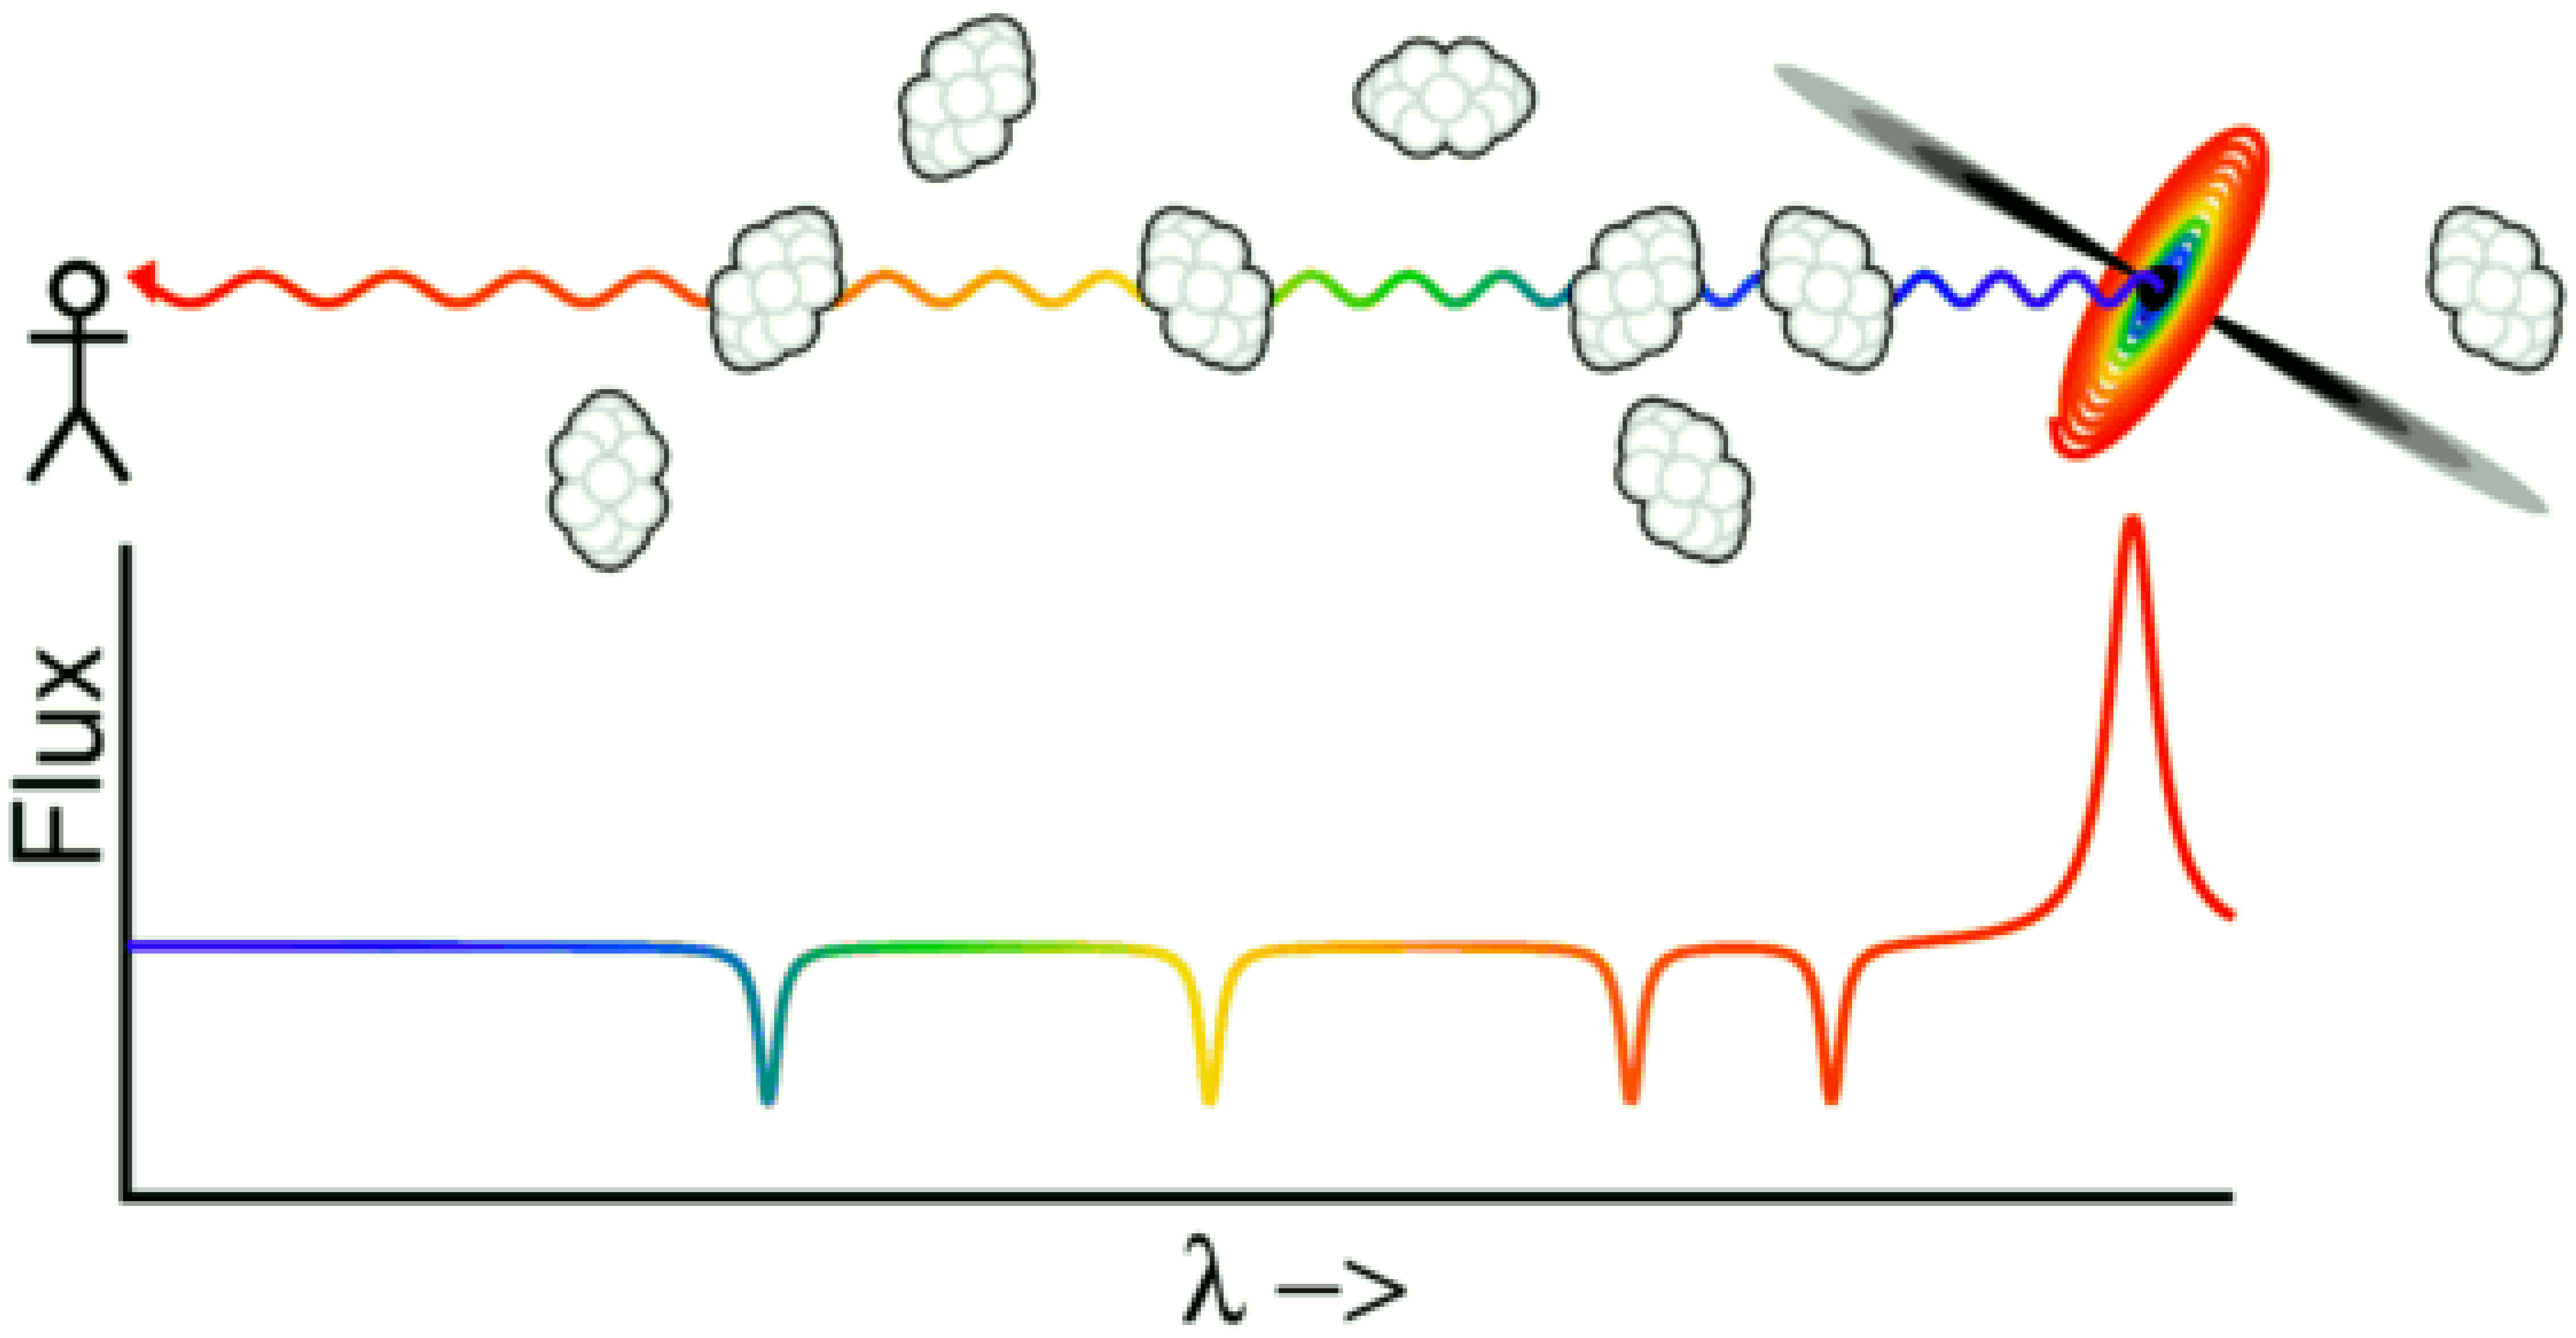
\includegraphics[width=12cm]{lyaf-75.eps}
  \caption{Illustration of the basic physics behind the \lya\ forest and how gas at different locations along the line of sight results in absorption lines at different wavelengths. (Image from {\tt http://www.astro.ucla.edu/})}
  \label{fig:LyaCartoon}
\end{figure}

The same logical progression also applies to the other lines in the Lyman-series. Therefore, you could imagine observing a \lyb\ and Ly\ $\gamma$\ forest at smaller wavelengths. There are a couple differences, however. First, lines deeper in the series have a smaller cross section for absorption, so intervening hydrogen will absorb less at these frequencies. Second, photons emitted from a background source with energies larger than \lyb\ will redshift through the \lyb\ wavelength and \textit{also} possibly through the \lya\ wavelength before reaching us and will have two opportunities to be absorbed. The photon's physical location when it redshifts through those two wavelengths will be completely different and, therefore, when observing absorption lines in the \lyb\ forest, it can be difficult to tell if the photons were absorbed by distant gas undergoing a \lyb\ transmission or closer gas undergoing a \lya\ transition. This problem is clearly exacerbated when considering higher-order lines since a larger number of distinct regions along the line of sight can contribute to the absorption.


We show two example quasar spectra in Figure \ref{fig:LyaExample}. The spectrum in the top panel is for a quasar at relatively low redshift and shows very little absorption. Meanwhile, the quasar in the bottom panel shows little absorption for emitted wavelengths redward of \lya\ but is heavily punctuated by absorption blueward of \lya\ due to intervening neutral hydrogen.
 
\begin{figure}[h]
  \centering
  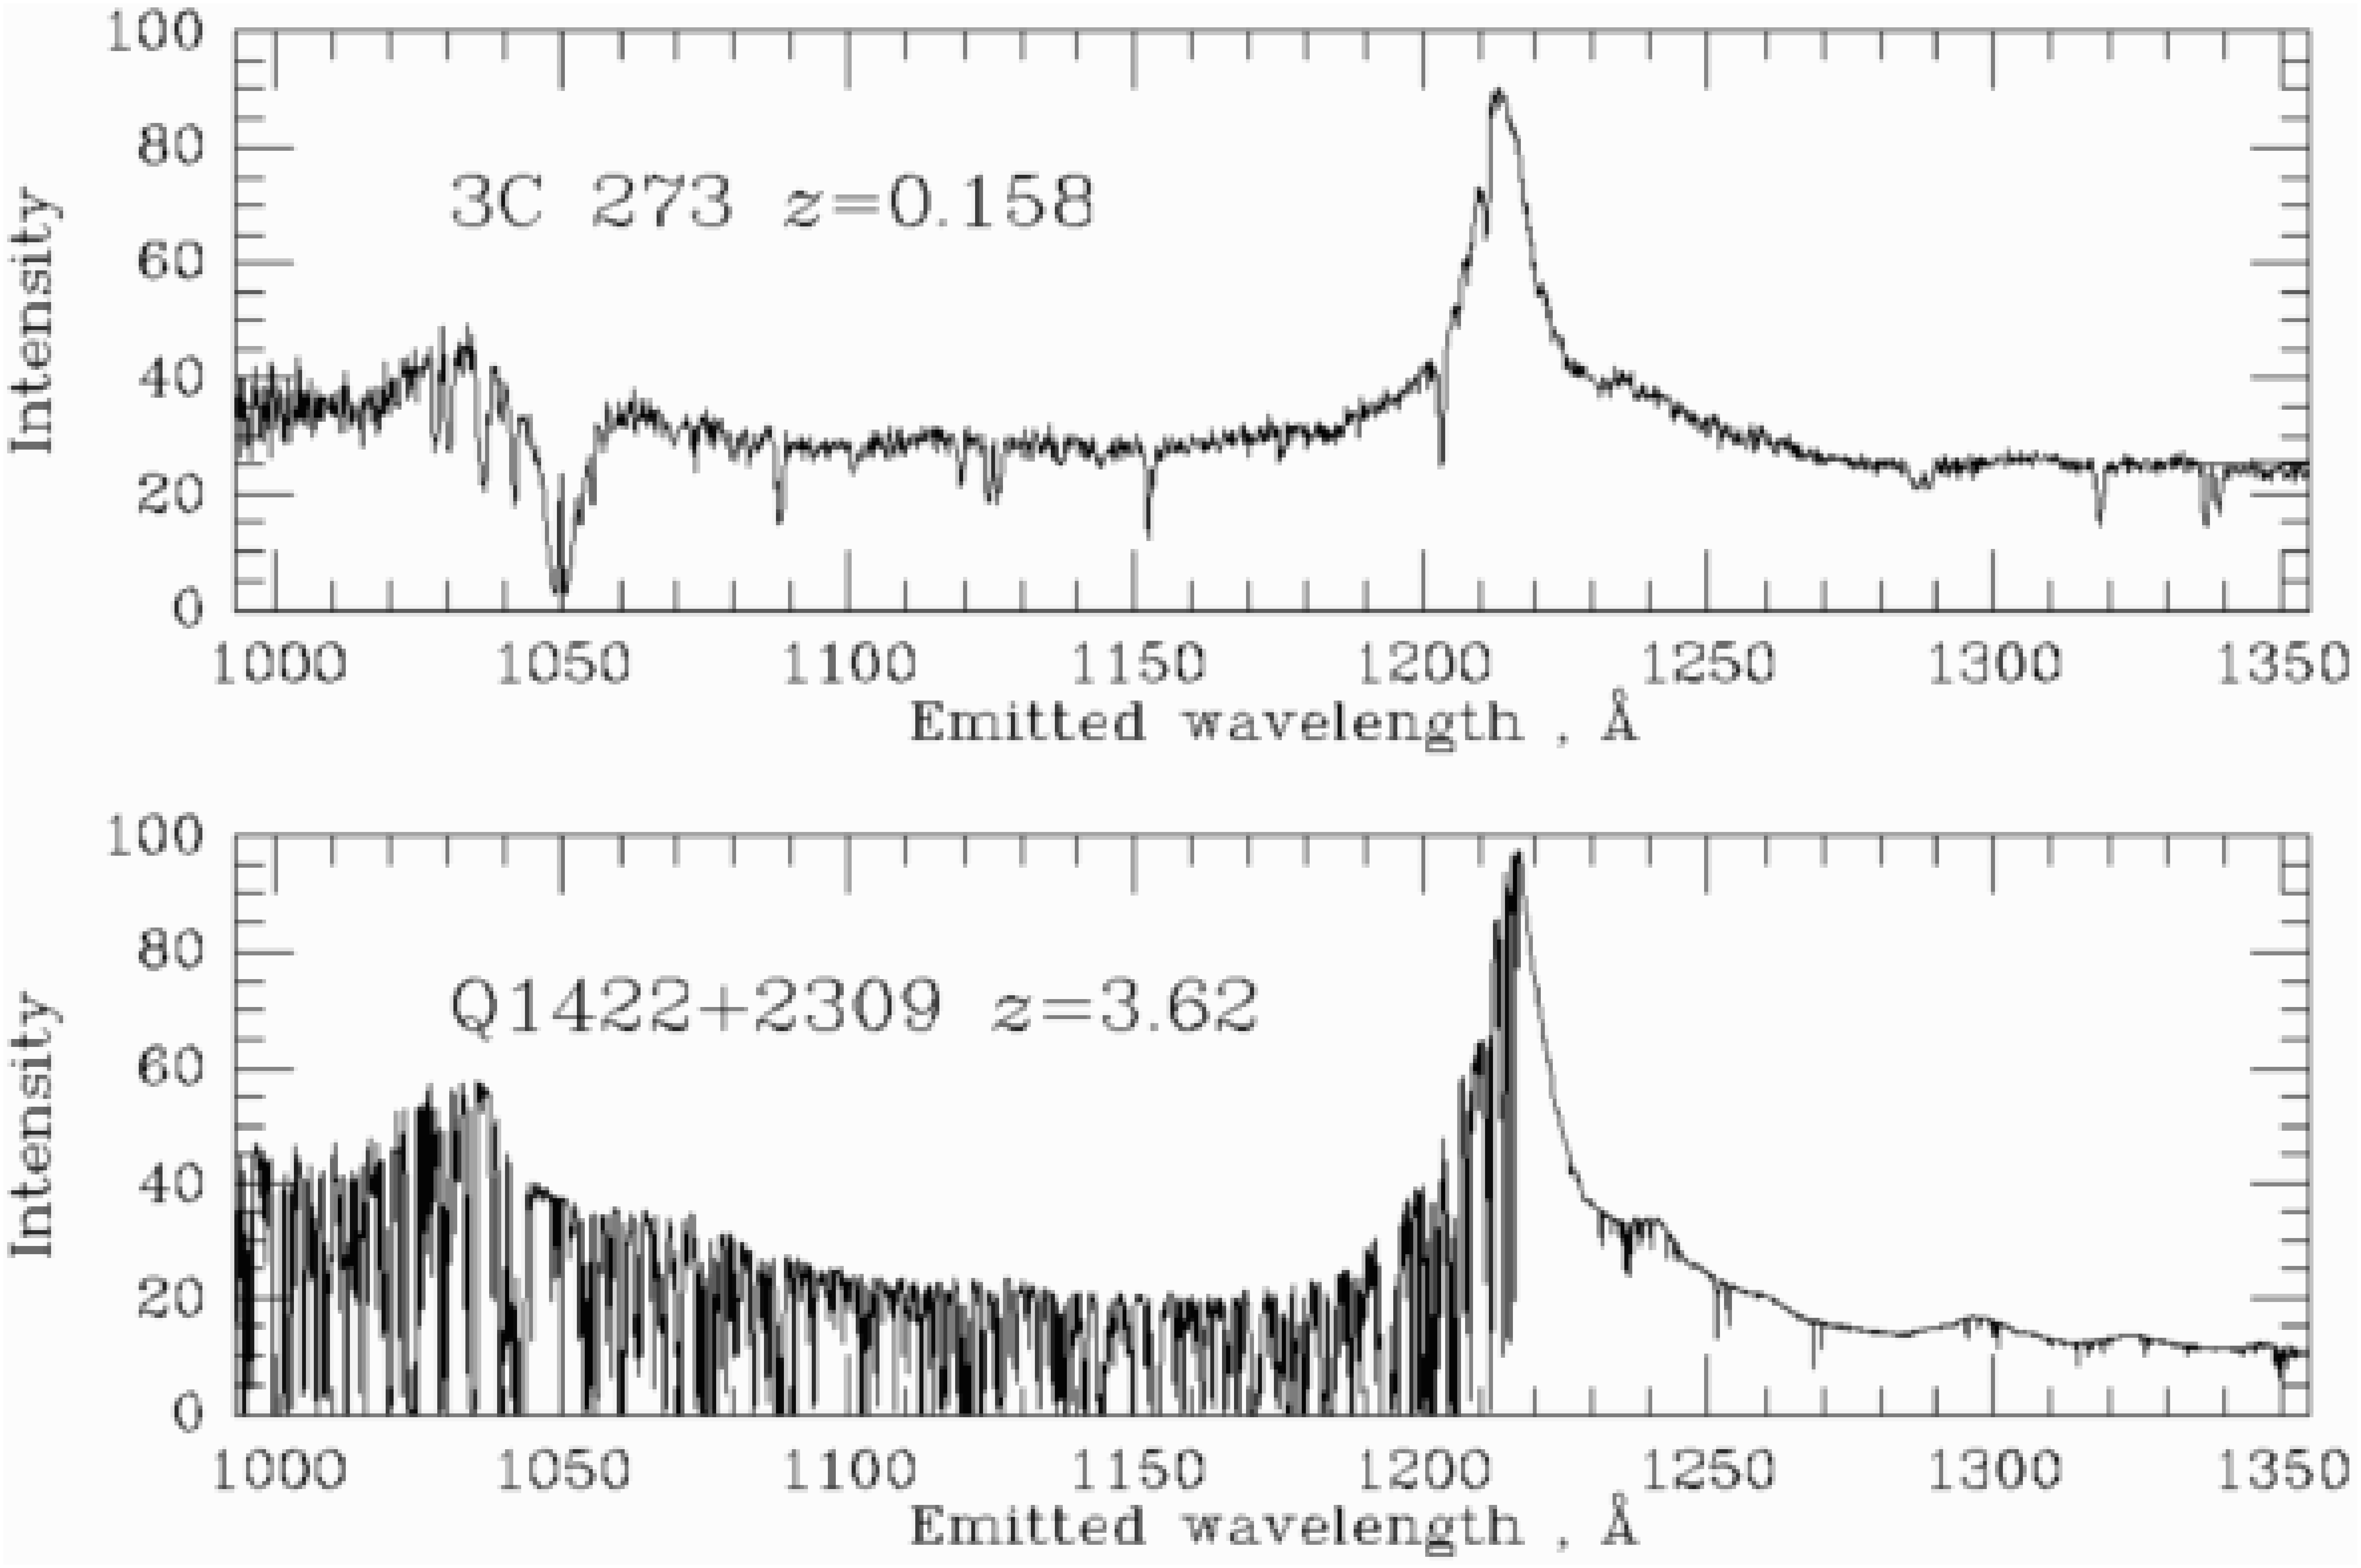
\includegraphics[width=12cm]{Lya-forest-60.eps}
  \caption{Flux as a function of rest-frame wavelength for a quasar at $z = 0.158$ (top) and $z = 3.62$ (bottom). The denser IGM at higher $z$ results in a dense ``forest" of absorption lines blueward of the rest-frame \lya\ line in the lower panel. (Image from {\tt http://www.astro.ucla.edu/})}
  \label{fig:LyaExample}
\end{figure}

At this point, the \lya\ forest should sound like a perfect tool: if we want to map the distribution of neutral hydrogen along the line of sight to a distant bright source, we can simply map each absorption line in the \lya\ forest to a parcel of neutral hydrogen. However, the story becomes complicated here due to the extremely large cross section for \lya\ absorption. Namely, the optical depth\nomenclature[Zp]{Optical Depth}{Optical depth, denoted by $\tau$, is a quantity that describes that likelihood for a photon to be absorbed, usually by a gas. The fraction of photons that will pass through the gas unabsorbed is $e^{-\tau}$.} for \lya\ absorption of a neutral hydrogen gas parcel is approximately

\begin{align}
\tau_{\alpha} &\approx 3.3 \times 10^{4} \xhi (1 + \delta) \left[\dfrac{1+z}{6.5}\right]^{3/2}. \label{eq:tauGP}
\end{align}

Using this expression, we can calculate the minimum neutral fraction needed for a gas parcel at mean density to allow 1\% transmission at $z = 5.5$:

\begin{align}
.01 &= e^{-\tau_{\text{min}}} \implies \tau_{\text{min}} \approx 4.6\\
4.6 &\approx \tau_{\alpha} x_{\text{HI,min}} \\
\implies x_{\text{HI,min}} &\approx 0.00014.
\end{align}


This reveals the fly in the ointment here: even a gas parcel that is 99.9\% ionized will allow less than 1\% transmission at the redshifts of interest for reionization. This allows absorption features to be caused by highly-ionized gas that happens to be over-dense. Therefore, we can not simply map absorption lines in the \lya\ forest to regions of significantly-neutral hydrogen. In fact, the second example quasar we see in Figure \ref{fig:LyaExample} shows significant \lya\ absorption and is located at $z = 3.62$, \textit{much later than the end of reionization}. At this point, the reader may ask what utility does the \lya\ forest have at all? Well, an enormous amount. To name a very few applications outside of reionization, since \lya\ absorption can be caused by matter overdensities, the \lya\ forest can be used to measure the matter power spectrum in the IGM. This, in turn, can be used to measure the baryon acoustic oscillations (BAO), provide lower limits on the mass of the dark matter (\citealt{Viel:2013fqw}), and constrain dark energy, for example. Additionally, absorption features due to damped \lya\ absorbers (DLAs) can be used to measure the primordial deuterium abundance as a test of big bang nucleosynthesis.\\
\textcolor{white}{suspense!}\\
\noindent But how to constrain the EoR?



\subsubsection{Evolution of $\tau_{\text{eff}}$}

% The Gunn-Peterson optical depth to \lya\ photons is \tau_{\text{GP}} = \dfrac{\pi e^2}{m_e c} f_{\alpha} \lambda_{\alpha} H^{-1}(z)n_{\text{HI}}

% Absorption is understood as being caused by the fluctuating Gunn-Peterson effect, low density regions in approximate thermal equilibrium between photoionization heating by the UV background and adiabatic cooling due to the Hubble expansion, rather than discrete \lya\ absorbers.

% By studying the evolution of the average transmitted flux or effective optical depth, one can trace the evolution in the 

% You probably want to re-read and refer to Lidz et al. that discuss that the evolution in the effective optical depth can be replicated by density fluctuations

Perhaps the most common analysis performed on high-redshift quasar spectra in the context of constraining the EoR is measurements of the effective Gunn-Peterson optical depth, defined as

\begin{align}
\langle F \rangle &\equiv e^{-\tau_{\text{eff}}}
\end{align}
\gloss{$\tau_{\text{eff}}$}{The effective Gunn-Peterson optical depth, which is the negative log of the mean transmission over a given redshift bin. Measurements of $\tau_{\text{eff}}$ are often converted into constraints on the photoionizaiton rate}where $\langle F \rangle$ is the averaged transmission fraction over a redshift bin in a quasar/GRB spectrum. Under the assumption of a uniform ionizing background and ionization equilibrium, where the rate that neutral hydrogen atoms are ionized is equal to the rate that ionized hydrogen atoms recombine, the effective optical depth encodes important information about the state of the IGM. In order to see this, we can take a few steps to express the optical depth in terms of the properties of the IGM.\footnote{The following discussion will borrow heavily from \cite{FaucherGiguere:2007jc} and \cite{fan2002evolution}.} First, the Gunn-Peterson optical depth can be expressed as

\begin{align}
\tau_{\text{GP}} &= \dfrac{\pi e^{2}}{m_{e} c} f_{\alpha}\lambda_{\alpha} \dfrac{n_{\text{HI}}}{H(z)}, \label{eq:tauGP}
\end{align}

where $H(z)$ is the Hubble parameter at redshift $z$, $e$ is the charge of the electron, $m_e$ is the electron mass, $c$ is the speed of light, $\lambda_{\alpha}$ is the \lya\ wavelength, $f_{\alpha}$ is the quantum mechanical oscillator strength, and $n_{\text{HI}}$ is the number density of neutral hydrogen atoms\gloss{HI}{Neutral hydrogen}\gloss{HII}{Ionized hydrogen}\gloss{HeI}{Neutral helium}\gloss{HeII}{Singly-ionized Helium}\gloss{HeIII}{Fully-ionized helium}\gloss{$f_{\alpha}$}{Quantum mechanical oscillator strength for the \lya\ transition}\gloss{$e$}{Charge of the electron}\gloss{$\lambda_{\alpha}$}{Wavelength of the \lya\ transition}\gloss{$m_e$}{Mass of the electron}. All of these quantities are known with the exception of the number density of neutral hydrogen atoms. To find this, we first utilize the statement of ionization equilibrium:

\begin{align}
\Gamma_{\text{HI}} n_{\text{HI}} &= R(T)n_{e}n_{\text{HII}} \label{eq:IonEquilibrium} \\
n_{\text{HI}} &= \dfrac{R(T) n_{e} n_{\text{HII}}}{\Gamma_{\text{HI}}} \label{eq:nH}\\
x_{\text{HI}} &= \dfrac{R(T)n_e}{\Gamma_{\text{HI}}} \label{eq:xHI}
\end{align}

where $\Gamma_{\text{HI}}$\gloss{$\Gamma_{\text{HI}}$}{Photoionization rate for hydrogen atoms. This depends on the number,  location, and properties of the ionizing sources.} is the photoionization rate due to the ionizing sources, $n_{e}$ is the number density of free electrons, $n_{\text{HII}}$ is the number density of ionized hydrogen atoms (protons), and $x_{\text{HI}}$ is the hydrogen neutral fraction. The left-hand side of Eq. \ref{eq:IonEquilibrium} represents the rate of photoionizations per volume and the right hand side represents the rate of hydrogen recombinations per volume. Under the assumption of ionization equilibrium with a uniform ionizing background, the presence of any transmission suggests $n_{\text{HII}} \approx n_{\text{HI}} + n_{\text{HII}} = n_{\text{H}}$ and 

\begin{align}
\bar{n}_{\text{H}} &= \frac{\rho_{c}(z)\Omega_{b}(z)X_{\text{H}}}{m_p} = \dfrac{3H^{2}(z)}{8\pi G} \dfrac{\Omega_{b}(z) X_{\text{H}}}{m_{p}} \\
&= \dfrac{3H_{0}^{2}\Omega_{b,0}}{8\pi G} \dfrac{X_{\text{H}}}{m_p}(1+z)^{3}\\
n_{\text{H}} &= (1+\delta) \bar{n}_{\text{H}}. \label{eq:ntot}
\end{align}

In this expression, $\rho_c$\gloss{$\rho_{c}$}{Critical energy density for a flat Universe} is the critical density for a flat Universe, $\Omega_{b}$\gloss{$\Omega_b$}{Baryon density in units of the critical density} is the baryon density in units of the critical density, $X_{\text{H}}$\gloss{$X_{\text{H}}$}{The fraction of baryonic mass in the form of hydrogen} is the fraction of baryonic mass in the form of hydrogen, $m_{p}$ is the mass of the proton which is effectively equal to the mass of the hydrogen atom, and $\delta \equiv (\rho-\bar{\rho})/\bar{\rho}$\gloss{$\delta$}{The local mass overdensity in units of the cosmic mean} is the local mass overdensity in units of the cosmic mean. A subscript of ``0" denotes that these are present-day values and $\bar{n}_{\text{H}}$ denotes the average of $n_{\text{H}}$. Thus, as we expect, this expression is essentially equal to the mass density of hydrogen atoms in the Universe divided by the mass per atom.\footnote{It may be interesting to note that this value corresponds to 0.2 hydrogen atoms per cubic meter today and roughly $\sim$50 hydrogen atoms per cubic meter at $z = 5.5$. It is very empty out there.}  The expression for the electron number density should be the same, since each ionized hydrogen atom releases one free electron. However, it is probably the case that helium is singly ionized along with hydrogen, so the number density will increase according to:

\begin{align}
\bar{n}_e &= \bar{n}_{\text{H}} + \bar{n}_{\text{He}} = \dfrac{3H^2}{8\pi G}\left( \dfrac{X_{\text{H}}}{m_{p}} + \dfrac{(1 - X_{\text{H}})}{4m_{p}} \right) \\
&\approx 1.08 \bar{n}_{\text{H}}. 
\end{align}

However, for simplicity here, let us approximate $n_{\text{tot}} \equiv n_{e} \approx n_{\text{H}}$. The quantity $R(T)$ in Eq. \ref{eq:IonEquilibrium} is the recombination rate, which is equal to (\citealt{Hui1997}):

\begin{align}
R(T) &\approx 4.2 \times 10^{-13}\left( \dfrac{T}{10^{4} K}\right)^{-0.7} \text{cm}^{3}\sec^{-1}. \label{eq:RecombinationRate}
\end{align}

For $\delta \lesssim 5$, \cite{Hui1997} showed that the temperature and density follow the relationship

\begin{align}
T &\approx T_{0}(1+\delta)^{\gamma - 1} \label{eq:Trelation}
\end{align}

where $T_0$ is the temperature of a parcel of gas at mean density, and $\gamma$ is the slope of the temperature-density relation. For compactness, let's define $R_{4} \equiv R(T=10^{4}K)$. At this point, we are ready to combine Eq. \ref{eq:Trelation}, \ref{eq:RecombinationRate}, \ref{eq:ntot}, \ref{eq:nH}, and \ref{eq:tauGP} to get an expression for $\tau_{\text{GP}}$:

\begin{align}
\tau_{\text{GP}} &= \dfrac{\pi e^2}{m_e c}\dfrac{f_{\alpha}\lambda_{\alpha}}{H(z)} \dfrac{R_{4}(1+\delta)^{-0.7(\gamma - 1)}\bar{n}_{\text{tot}}^{2}(z)(1+\delta)^2}{\Gamma_{\text{HI}}}\\
&= \dfrac{\pi e^2}{m_e c}\dfrac{f_{\alpha}\lambda_{\alpha}}{H(z)} \dfrac{R_4 \bar{n}_{\text{tot}}^{2}(z)}{\Gamma_{\text{HI}}} (1+\delta)^{2-0.7(\gamma-1)}. \label{eq:tauGPfinal}
\end{align}

Finally, we have an expression for the \lya\ optical depth in terms of several properties of the IGM. The primary unknown in the above expression is the photoionization rate, which is a very complicated parameter which depends on the number, intensity, spectrum, and proximity of ionizing sources among other things. A common assumption in these types of analyses is that the photoionization rate is approximately spatially uniform. This seems like a plausible assumption in a post-reionization Universe, when the mean free path of ionizing radiation is long allowing any given gas parcel can receive ionizing radiation from many sources. On the other hand, early in reionization, the Universe is opaque to ionizing radiation and gas parcels tend to only see sources within their own ionized regions. Regardless, with this approximation, the observed mean transmission in a region of the spectrum is akin to an average of Eq. \ref{eq:tauGPfinal} marginalizing over the density field:

\begin{align}
\left\langle F \right\rangle &= \int \dd \delta\ e^{-\tau(\delta)} P(\delta) \equiv e^{-\tau_{\text{eff}}}.
\end{align}


 As such, an intriguing question is, if you have a model for the probability distribution of the underlying density field, what (uniform) value of $\Gamma_{\text{HI}}$ will yield a value for $\left\langle F \right\rangle$ that is consistent with observations? This question has received a lot of attention ({\bf cites}) and has led to many measurements of the photoionization rate. With estimates of the photoionization rate in hand, we can utilize Eq. \ref{eq:xHI} in order to obtain measurements of the IGM neutral fraction in each redshift bin in the spectra in order to gauge the progress of the EoR. Results for measurements of $\Gamma_{\text{HI}}$ and $\axhi$ via this method, performed by \cite{Fan2006a}, are shown in Figure \ref{fig:tauEffResults}. This figure demonstrates that, using $\tau_{\text{eff}}$ and the assumption of ionization equilibrium, estimates of the neutral fraction are exceedingly small for $z \lesssim 6$. This argument has played a large part in forming the common knowledge that reionization has ended by $z = 6$. 

\begin{figure}[h]
  \centering
  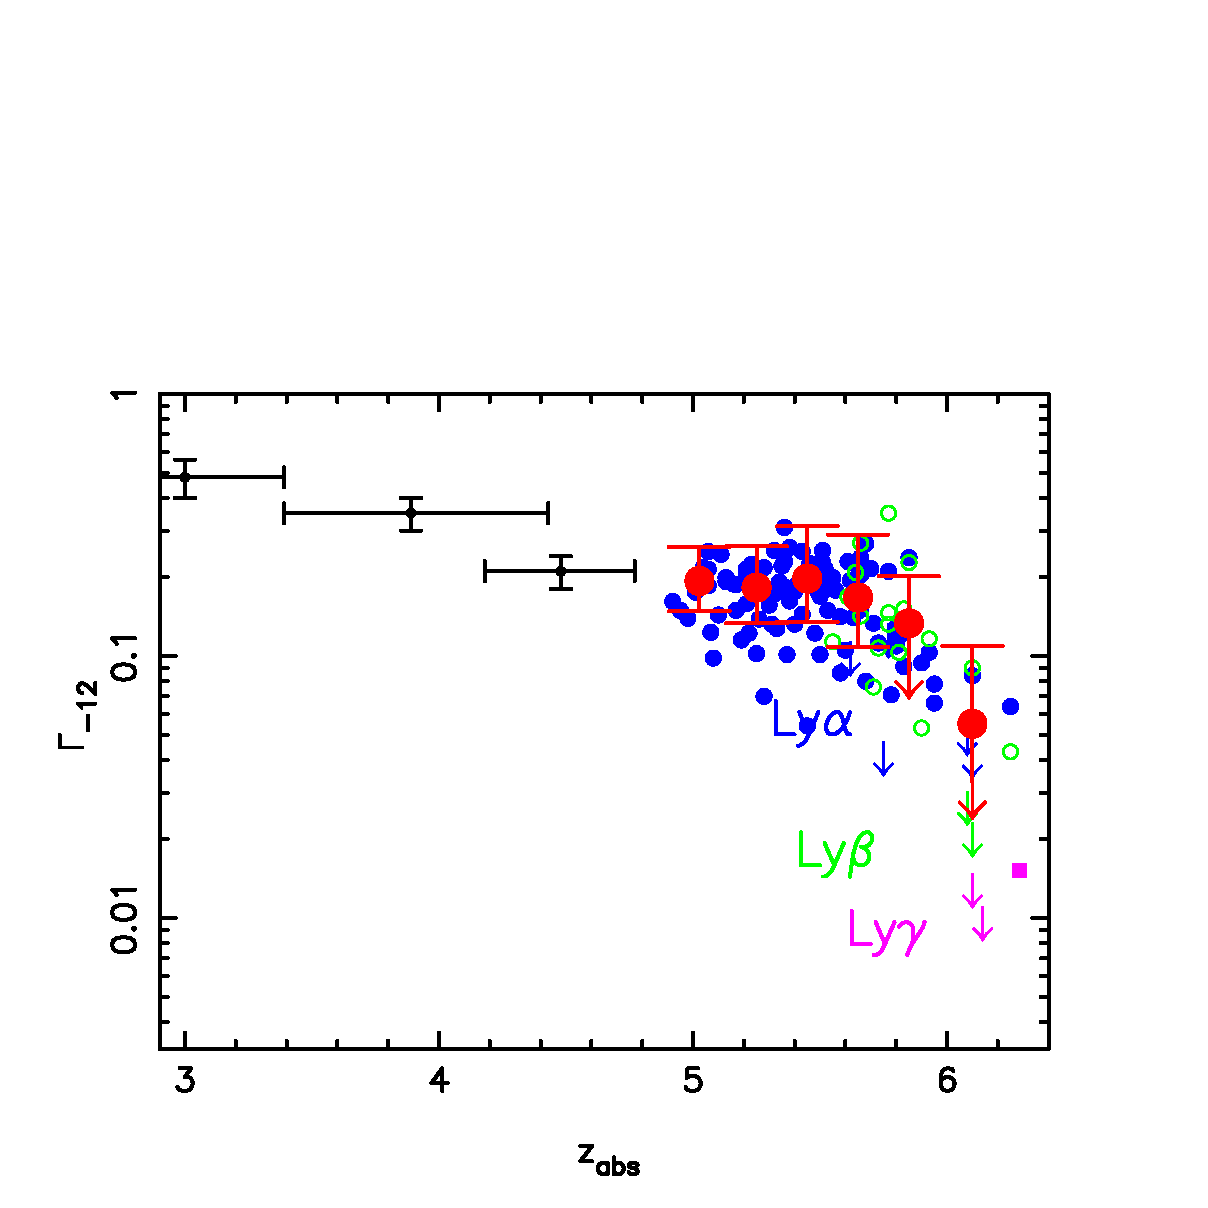
\includegraphics[width=8cm]{Fan.gamma.eps}
  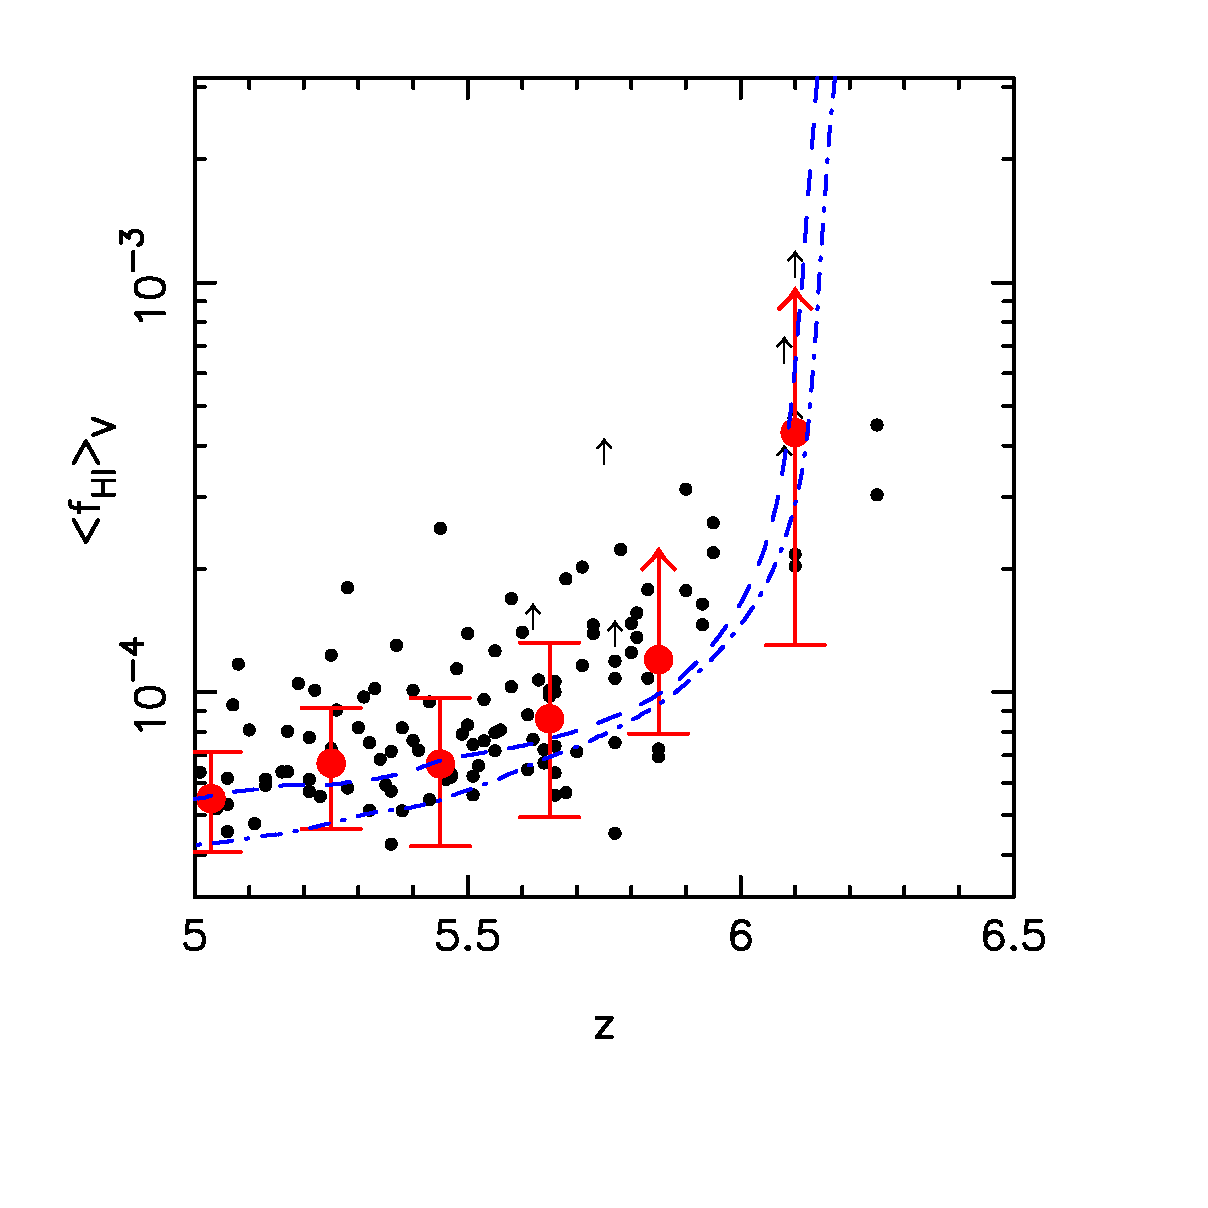
\includegraphics[width=8cm]{Fan.fHv.eps}
  \caption{Measurements of $\Gamma_{\text{HI}}$ (top) and $\axhi$ from \cite{Fan2006a} (bottom).}
  \label{fig:tauEffResults}
\end{figure}


Despite the widespread analysis of $\tau_{\text{eff}}$ in constraining the end of reionization, the interpretation of $\tau_{\text{eff}}$ is quite complicated.\footnote{For a more thorough discussion of controversial aspects of these constraints, see the intro for \cite{McGreer:2011dm}.} First, accepting the assumption of the IGM being in ionization equilibrium with a uniform $\Gamma_{\text{HI}}$ is tantamount to assuming that reionization has ended. Specifically, as discussed in \S \ref{sec:CosmicContext}, reionization is likely a highly inhomogeneous process with ionized bubbles forming around the brightest sources, growing, and eventually overlapping. During the period prior to complete overlap, regions of neutral hydrogen will be shielded from the ionizing radiation while ionized bubbles will experience a very large $\Gamma_{\text{HI}}$. This is not reflected in Eq. \ref{eq:IonEquilibrium} and so we expect conclusions derived from this method to be unreliable when we begin to push up against the end of reionization. Additionally, interpretation of the level of flux in quasar spectra in the context of reionization is further complicated by the fact that quasars likely reside in very atypical parts of the Universe. Specifically, \cite{Lidz:2007mz} show that it is likely that some quasar lines of sight will pass through mostly ionized gas even up to neutral fractions of $\axhi \sim 0.5$. 

%\subsubsection{Dark Gap Sizes}
%
%Yeah, so the main point we want to (briefly) drive home here is that previous constraints on $\axhi$ from the use of dark gap statistics probably assumed a uniform $\Gamma_{\text{HI}}$, which is equivalent to assuming reionization has already ended anyway. 
%
%Fan says imperfect sky subtraction in regions with strong OH lines can cause significant residuals resulting in an \textit{underestimate} in the dark gap size. Although, it seems like they don't allow any room for noise fluctuations in what they constitute a dark gap???


\subsubsection{Dark Pixel Covering Fraction}

As demonstrated in the previous section, interpreting measurements of the effective optical depth in the context of reionization is complicated and can rely on controversial assumptions. However, an alternative approach is to consider what constraints can be made without resorting to such assumptions. In this regard, an important method in estimating $\axhi$ from high-redshift quasar observations is the dark pixel covering fraction. This approach is rooted in the fact that neutral parcels of gas are certain to result in saturated absorption in quasar spectra due to their optical depths being $\tau_{\text{HI}} \gtrsim 10^4$ (Eq. \ref{eq:tauGP}). Therefore, a reliable upper bound on the neutral fraction at a given redshift can be estimated by the fraction of pixels in quasar spectra that are completely absorbed at that redshift. 

An obvious drawback of this method is that, at $z \sim 6$, overdense yet ionized regions will also result in saturated absorption and will significantly increase this upper bound on the neutral fraction. One approach to combat this effect is to incorporate the \lyb\ forest into the analysis. The optical depth for Lyman-series transitions scales as $f\lambda$, where $f$ is the oscillator strength of the transition and $\lambda$ is the corresponding wavelength. Therefore, the analogous expression of Eq. \ref{eq:tauGP} for \lyb\ is:

%Useful quantities:                                                                                                   
% Oscillator Strengths                                                                                                
% f_21 = 0.4162 (1s-2p)  lambda_21 = 1215.67 AA                                                                       
% f_31 = 0.0791 (1s-3p)  lambda_31 = 1025.72 AA                                                                       
% f_32 = 0.4349 (2s-3p)  lambda_32 = 6562.74 AA 
\begin{align}
\tau_{\beta} &= \tau_{\alpha} \times \dfrac{f_{\beta}\lambda_{\beta}}{f_{\alpha}\lambda_{\alpha}} \approx 5.3 \times 10^{3} \xhi (1 + \delta) \left[\dfrac{1+z}{6.5}\right]^{3/2}. \label{eq:tauGPB}
\end{align}

where $f_{\alpha} = 0.4162$, $\lambda_{\alpha} = 1216 \AA$, $f_{\beta} = 0.0791$, and $\lambda_{\beta} = 1026\AA$. From this expression, we can see that a mean-density parcel of neutral gas should cause saturated absorption in both the \lya\ and \lyb\ transitions. Meanwhile, ionized overdense regions are less likely to cause saturated absorption as their optical depth in \lyb\ is reduced by a factor of $f_{\beta}\lambda_{\beta}/f_{\alpha}\lambda_{\alpha} \approx 1/6$. Therefore, limits from the dark-pixel covering fraction may be improved by requiring simultaneous absorption in both \lya\ and \lyb\ as part of the definition of a dark pixel. Additionally, the \lyb\ dark pixel covering fraction on its own is a viable tool for establishing an upper bound on the neutral fraction, although foreground \lya\ absorption may undo some of the gains from the lower $\tau_{\beta}$ value. In practice, all three approaches (requiring \lya, \lyb, and \lya +\lyb\ absorption) are used. 

This procedure faces several complications when actually carried out, however. First, quasar observations are subject to the noise from the night sky which effectively adds mean-zero random noise to the spectra. The addition of this random noise can result in spurious transmission in pixels that otherwise would have been completely absorbed. Therefore, to measure the dark pixel fraction in quasar spectra, one first needs to create a suitable definition of what qualifies as a ``dark" pixel. One approach here is to define dark pixels as having transmission below some threshold defined in terms of the noise standard deviation, $\sigma_{\text{N}}$. This presents us with a tradeoff, however, since larger thresholds will reduce the number of neutral pixels we miss but also increase the number of ionized pixels that get incorporated into the dark pixel population. Alternatively, if we are presented with median-zero noise, then half of all truly-absorbed pixels will result in negative flux values, on average. This presents the possibility of using twice the negative-flux-pixel covering fraction as an estimate of the dark-pixel covering fraction (or four times, in the case of requiring \lya +\lyb\ absorption) (\citealt{McGreer:2014qwa}). 

A second complication is that, since pixels have a finite width, their transmission values effectively represent an average of the transmission over some region in the spectra. If the pixel width is large enough, then it is possible for a pixel to have non-zero transmission despite corresponding to a physical region that contains significantly-neutral gas. For example, if the physical region in space associated with the pixel is 80\% composed of completely-neutral gas and 20\% composed of completely ionized gas which allows full transmission, then the transmission of that pixel will be 20\% and will likely not qualify as a ``dark pixel" despite containing neutral gas. Thus, even in a measurement as seemingly-simple as the dark-pixel covering fraction, these details must be kept in mind when interpreting results. 

Regardless, \cite{McGreer:2011dm} and \cite{McGreer:2014qwa} apply the dark-pixel covering fraction approach to 22 high-redshift quasar spectra to produce the constraints on $\axhi$ shown in Figure \ref{fig:McGreer}. Dimly-colored points correspond to \cite{McGreer:2011dm} while bold-colored points correspond to \cite{McGreer:2014qwa}. These results present a very different interpretation than using $\tau_{\text{eff}}$ measurements while using the same data. Namely, that model-independent constraints have a hard time conclusively confirming the common knowledge that reionization has ended by $z \sim 6$.\footnote{The authors here do go on to focus on a high-resolution subset of their quasar observations presented in \cite{McGreer:2014qwa} in order to argue in favor of an end to the EoR by $z \sim 6$. However, the precise interpretation of the spectra is complex, as discussed herein.} 

\begin{figure}[h]
  \centering
  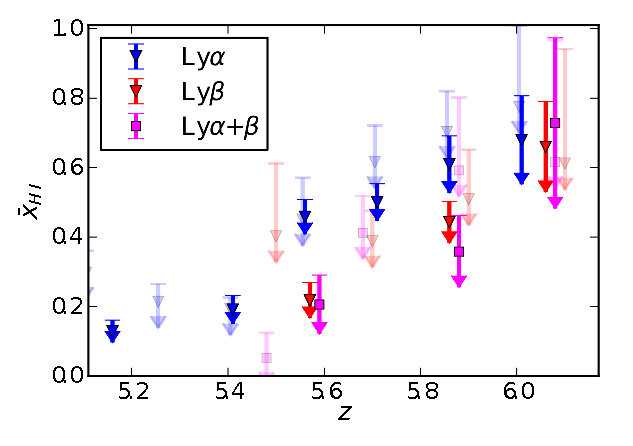
\includegraphics[width=8cm]{xhi_newdata.eps}
  \caption{Current limits on $\axhi$ derived from the dark-pixel covering fraction in \cite{McGreer:2014qwa}. Lightly-shaded points are older limits obtained in \cite{McGreer:2011dm}.}
  \label{fig:McGreer}
\end{figure}



\subsubsection{Damping Wing Redward of \lya}\label{sec:IntroDampingWing}

Much of the difficulties in using the \lya\ forest to constrain the timing of the EoR can be boiled down to the following problem: interpreting \lya\ absorption in high-redshift quasar spectra is difficult because both neutral and ionized gas can result in saturated absorption. Therefore, it is worth asking if there are any ways to break this degeneracy in \lya\ absorption in order to determine which absorption is likely due to neutral hydrogen. One potential approach toward this goal, which has received much attention (\citealt{Chornock:2013una}, \citealt{Chornock:2014fva}, \citealt{Mortlock2011}, \citealt{Bolton:2011vb}), is looking for the hydrogen damping wing redward of the \lya\ line. 


To understand this approach, let us first understand what the hydrogen damping wing is. For many applications, it is suitable to consider an atom's ability to absorb radiation as a series of delta functions in frequency: when incident radiation has a frequency exactly coinciding with the energy of the transition, then there is a non-zero probability for absorption and zero probability otherwise. In reality, the probability of absorbing a photon of a given frequency, e.g., the line profile, is a continuous distribution which, while small for frequencies $\nu \neq \nu_{0}$, is non-zero. 


The intrinsic line profile for the \lya\ transition in the hydrogen atom can be seen as arising from the time/energy uncertainty principle, $\Delta E \cdot \Delta t \gtrsim \hbar$. Specifically, the finite lifetime of the $n = 2$ excited state implies the existence of a range of energies that can excite, or result from, the transition. The distribution of this range of energies follows a Lorentzian distribution\gloss{Lorentzian Distribution}{Probability distribution for the ratio of two standard-normal-distributed variables. This distribution also describes the intrinsic line profile for absorption lines.}:\footnote{A quantum-mechanical discussion of this result can be found in \S 5.8 of \cite{sakurai2011modern}. A classical derivation can be found in \S 3.6 of \cite{rybicki1979radiative}.}

\begin{align}
\phi(\nu) &= \frac{1}{\pi} \dfrac{\Gamma/4\pi^{2}}{(\nu - \nu_{0})^{2} + (\Gamma/4\pi)^2}
\end{align}

with the corresponding absorption cross section

\begin{align}
\sigma_{\alpha}(\nu) &= \dfrac{\pi e^2}{m_{e}c} f_{\alpha} \phi(\nu). \label{eq:IntroLineProfile}
\end{align}

The ``damping wing" refers to the $\sigma \sim 1/(\nu-\nu_{0})^{2}$ behavior far from line center. This can be used to break the degeneracy between HII absorption and HI absorption because the optical depth is so much smaller in the damping wing that, without significantly-neutral gas (optical depth scales with neutral fraction), the optical depth at such frequency separations will not be sufficient to cause absorption. Furthermore, the damping wing has a distinct shape which can be fit for in order to infer the properties of the neutral gas which sources it. 


While the damping wing from an isolated neutral region in a sea of fully-ionized, $\tau = 0$ hydrogen would stand out like a sore thumb, in reality absorption from the surrounding dense, yet ionized, gas will punctuate the damping wing with additional absorption features and will make it harder to detect. This makes the prospect of looking for isolated damping wings in typical regions in quasar spectra unappealing. However, photons emitted slightly \textit{redward} of \lya\ cannot be absorbed by dense ionized gas since ionized gas has a negligible optical depth for $\nu \neq \nu_{\alpha}$. Neutral hydrogen, on the other hand, \textit{will} allow absorption to take place redward of \lya\ due to the significant optical depth in the damping wing. Because of this, searches for the damping wing slightly redward of the \lya\ line will be able to avoid nuisance absorption from neighboring ionized gas.


We show a famous example of a potential damping-wing detection in Figure \ref{fig:Mortlock}, taken from \cite{Mortlock2011}. This shows a region of the transmission spectrum for a quasar at redshift $z = 7.085$ (ULAS J1120+0641). The fractional transmission nearby the \lya\ line exhibits a gradual recovery from almost complete absorption at $\lambda < \lambda_{\alpha}$ to almost complete transmission at $\lambda > \lambda_{\alpha}$, occurring over a wavelength interval consistent with a hydrogen damping wing. The curves in blue show models for damping wing absorption associated with an IGM with neutral fraction $\axhi = 0.1$ (top), 0.5 (middle), and 1 (bottom) with a sharp ionization front at a distance of 2.2Mpc from the quasar. In green, a model for the absorption profile of a Damped \lya\ Absorber (DLA, see glossary for definition)\gloss{DLA}{Damped \lya\ Absorber. These are dense, isolated clouds of gas with extremely high column densities of neutral hydrogen, $N_{\text{HI}} \gtrsim 2\times10^{20}\cm^{-2}$ sufficient to exhibit damping-wing absorption. These are thought to source galaxy formation and are not part of the diffuse IGM which we want to study for reionization purposes.} with column density $N_{\text{HI}} = 4\times10^{20}\text{cm}^{-2}$ located 2.6 Mpc from the quasar is shown. Thus, the transmission profile appears consistent with both a significantly-neutral ($\axhi > 0.1$) IGM or a proximate DLA. However, \cite{Simcoe} perform a search for metal lines, which typically accompany DLA absorption, and find that the gas is extremely metal-poor. This bolsters the claim that the damping-wing absorption seen in this example is, in fact, due to diffuse neutral hydrogen in the IGM. 


\begin{figure}[h]
  \centering
  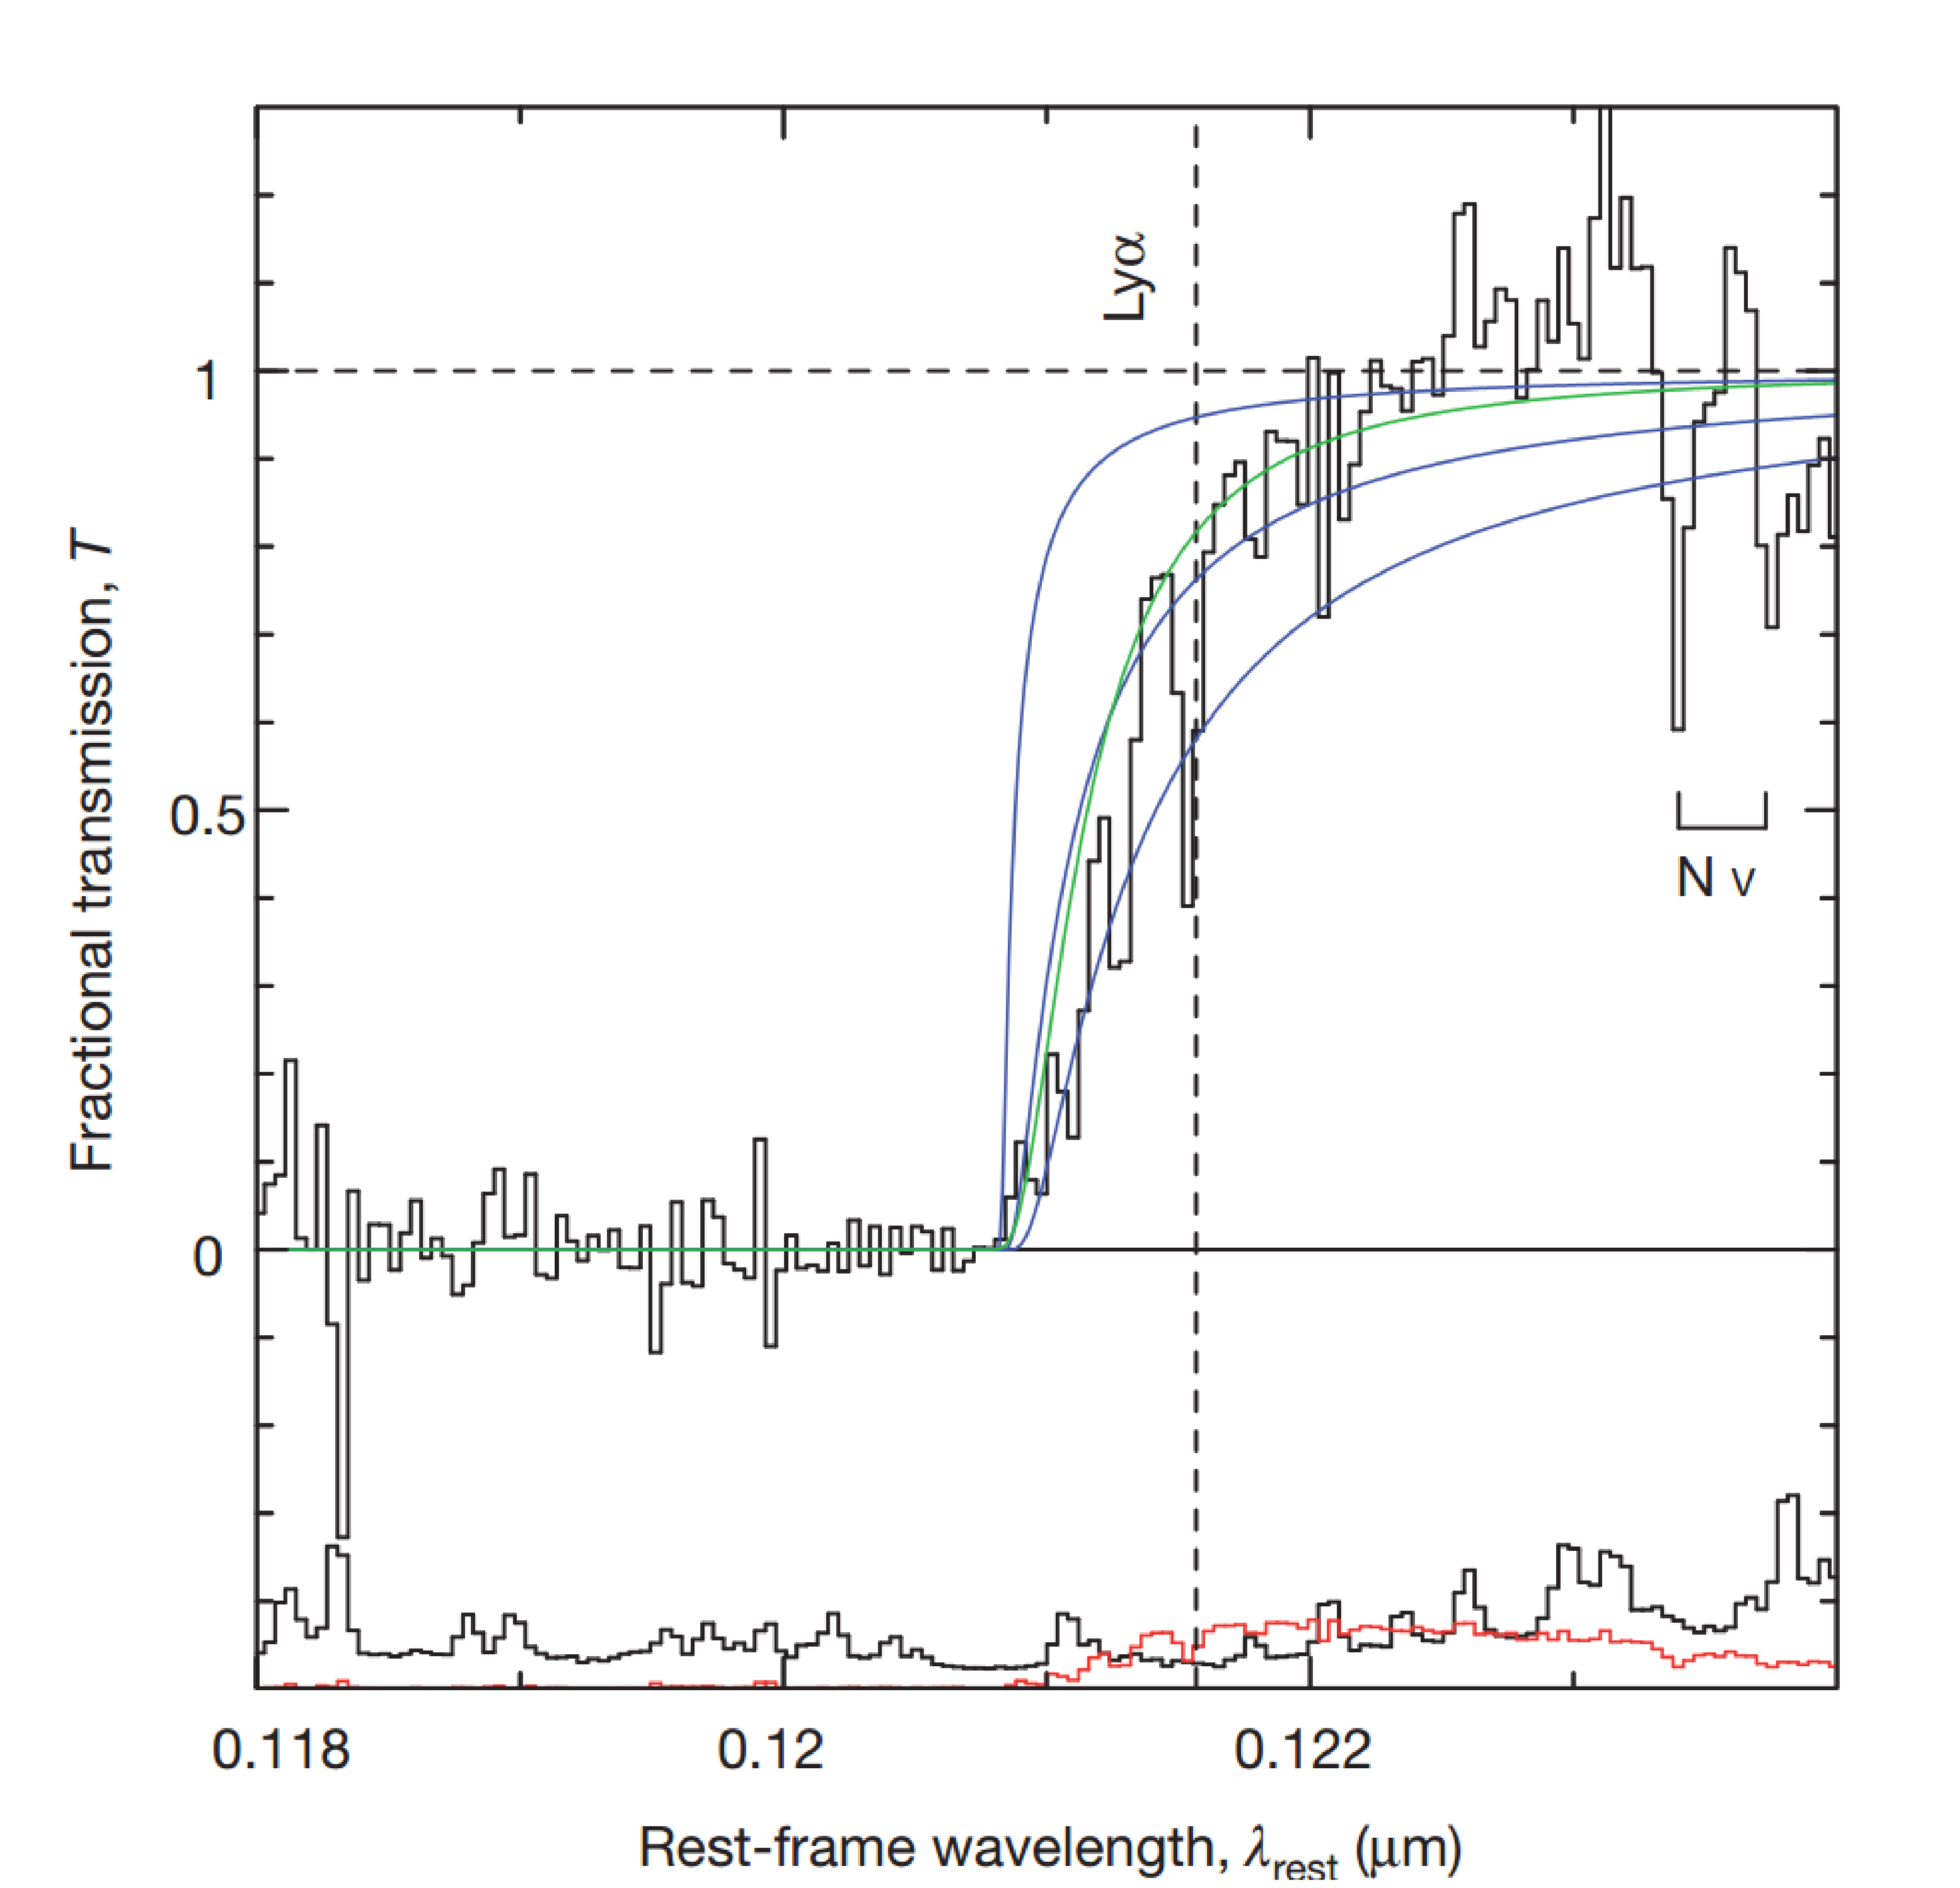
\includegraphics[width=8cm]{z7p085_DampingWing.eps}
  \caption{Quasar ULAS J1120+0641 identified at redshift $z = 7.085$ along with several fits for the damping wing.}
  \label{fig:Mortlock}
\end{figure}


Other searches for damping-wing absorption redward of \lya\ have been carried out on, for example, GRB 130606A (\citealt{Chornock:2013una}) and GRB 140515A (\citealt{Chornock:2014fva}). These authors looked for the damping wing in the spectra of GRB afterglows at redshift $z = 5.913$ and $z = 6.33$, respectively. A non-detection in the spectra of the $z = 5.913$ GRB allowed the authors to place a $2\sigma$ limit on the nearby IGM neutral fraction of $\axhi < 0.11$. Similarly, no strong evidence of a damping wing was found in the spectrum of GRB140515A, shown in Figure \ref{fig:GRB140515A}. The right-hand panel shows the transmission fraction nearby the \lya\ transition, which is equally-well fit by pure host absorption (blue, $N_{\text{HI}} = 10^{18.62}\text{cm}^{-2}$), pure IGM absorption from gas at $6.0 \leq z \leq 6.328$ with $\axhi = 0.056$ (red), and a hybrid model with a host absorber lying within an ionized bubble with $R = 10$ comoving Mpc met by an IGM with $\axhi = 0.12$ (green). As such, they argue against a significantly-neutral IGM at this redshift.  

\begin{figure}[h]
  \centering
  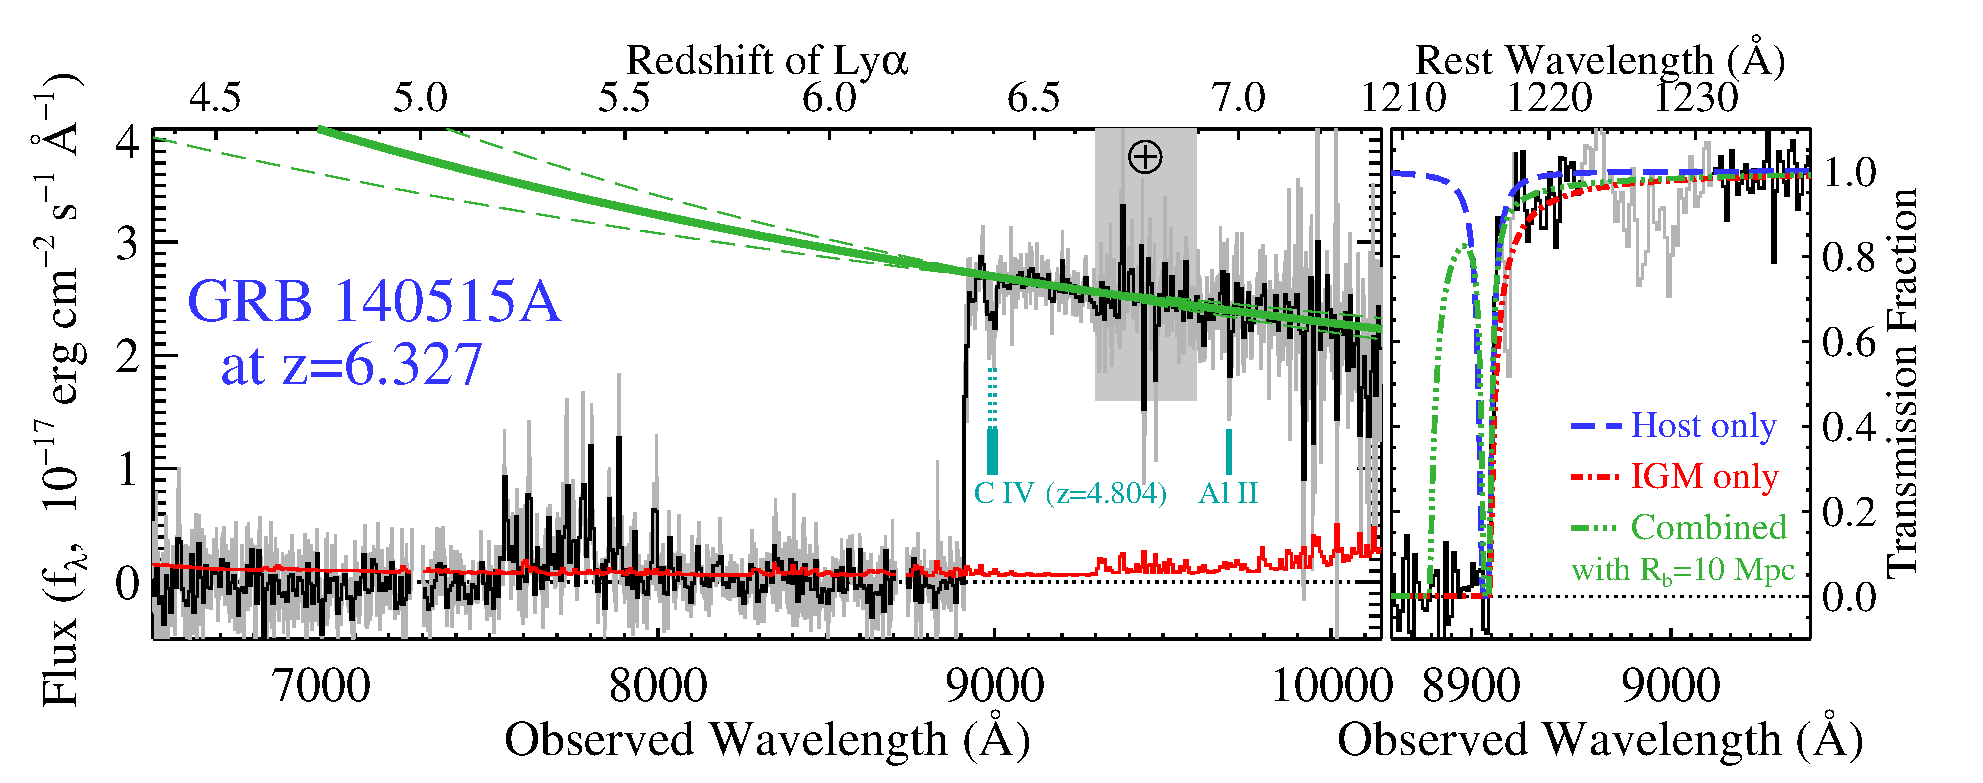
\includegraphics[width=14cm]{GRB140515A.eps}
  \caption{Spectrum of GRB140515A, a gamma-ray burst located at $z = 6.33$. The right-hand panel overlays damping wing models from a host absorber (blue), a pure IGM model with $\axhi = 0.056$ (red), and a combination model (green). The authors argue that, while each curve provides an equally-good fit to the data, the sharp rise in transmission shown is inconsistent with a significantly-neutral IGM. }
  \label{fig:GRB140515A}
\end{figure}


It is worth pointing out, however, that the method of searching for the damping wing redward of \lya\ is not without drawbacks. First, detecting the damping wing redward of \lya\ relies on your ability to understand what the quasar flux \textit{would have} been in the absence of the absorbing gas nearby the \lya\ line (this unabsorbed flux is referred to as the quasar \textit{continuum} and predicting the unabsorbed flux for a given quasar is called \textit{continuum fitting}). Predicting the \lya\ line properties in quasars is notoriously complicated and so modelling the precise fractional transmission must be done with care. Second, searching for the damping wing redward of \lya\ inherently involves measuring the gas properties nearby the quasar. However, quasars are extremely rare and special objects and it is not obvious that their surroundings are representative of the IGM on average. For example, \cite{Lidz:2007mz} found that quasars are likely born into large galaxy-generated ionized regions, suggesting that interpreting the \textit{lack} of a damping wing detection is not straightforward. Gamma-ray burst spectra are gaining attention in this regard (See \citealt{Salvaterra:2015gpa} for a review) as they tend to occupy more typical regions of space and have an easier-to-model continuum flux. The drawbacks of GRBs, though, is that they are often accompanied by a host absorber whose damping-wing absorption must be separated from that of the IGM. Third, even when provided with a clean detection of the damping wing redward of \lya, this will only tell you about one region of space and it will be difficult to use this single observation to extrapolate to the ionization state of the IGM as a whole. Later in this work, we propose a technique for searching for the hydrogen damping wing which, while faced with its own difficulties, is able to avoid the difficulties mentioned above. 

%Alternatively, the line profile for the hydrogen atom can be calculated classically by treating the electron as being harmonically-bound in the potential of the proton. The oscillations of the electron are intrinsically damped due to the fact that accelerating charges emit radiation. Furthermore, when we consider the probability of incident radiation being absorbed, the incident radiation can be seen as a driving force for the oscillator. 


% There is always a small damping of the oscillations by the radiation reaction force. I think this basically means that, since the charge is accelerating, it must be emitting radiation and losing energy and therefore its motion must be damped. Tau in this context is the time for radiation to cross a distance comparable to the size of the classical electron radius

\subsubsection{IGM Temperature}\label{sec:IntroIGMTemperature}

A detection of a damping wing redward of the \lya\ line in a quasar spectra would constitute a ``smoking gun" for significantly-neutral regions in the IGM, provided you could rule out the possibility of a DLA source. However, in the absence of a smoking gun, a \textit{warm} gun could be an indication of reionization having completed recently. Specifically, measurements of the IGM temperature can provide us with additional insights about the process of reionization. During reionization, patches of gas will be heated as they are ionized with their subsequent temperature only depending on the shape of the ionizing spectrum. Furthermore, once ionized, the thermal behavior of the gas is relatively simple: it will cool adiabatically as the Universe expands. Additional sources of heating, such as photo-heating from the ionization of the trace amounts of neutral hydrogen, and additional sources of cooling, such as Compton cooling off of CMB photons, will be insignificant. Because of this relatively simple cooling behavior, it should be possible to turn a measurement of the temperature of the IGM into a constraint on the timing of reionization. In order to do this, we need two main ingredients: a method of measuring the temperature of high-redshift gas and an understanding of how the temperature of the gas evolves with time after being ionized. 


One popular method for determining the temperature of the IGM utilizes the width of absorption lines in the \lya\ forest. In \S \ref{sec:IntroDampingWing}, we described the line profile for \lya\ absorption as obeying a Lorentzian distribution. While this is technically correct for any given atom, in reality, the atoms themselves have random thermal motions according to their temperature and will therefore see incident radiation as being redshifted or blueshifted accordingly.\footnote{The following discussion of Doppler broadening and the derivation of the Voigt profile closely follows notes taken from Masao Sako's ``Radiative Transfer" class offered in the Spring of 2010.}  As such, a hydrogen atom travelling \textit{toward} a photon with frequency just shy of the \lya\ frequency will see the light redshifted and can increase the chance of absorption. The effect of this is that the line profile for \lya\ absorption from a gas parcel gets smeared out, or, more precisely, gets convolved the with Maxwell-Boltzmann distribution. The greater the temperature, the greater the extent of this smearing. The Maxwell-Boltzmann distribution describes the velocities of particles in an ideal gas with a given temperature:


\begin{align}
W(\xi)\dd \xi &= \left( \dfrac{m_p}{2\pi k_{B}T} \right)^{1/2}e^{-m_p\xi^2/2 k_B T}\dd \xi \\
&= \left(\pi \xi_{0}^{2} \right)^{-1/2} e^{-\xi^{2}/\xi_{0}^{2}} \dd \xi \\
\xi_{0} &\equiv \sqrt{ \dfrac{2k_B T}{m_p}}
\end{align}


\begin{figure}[h]
  \centering
  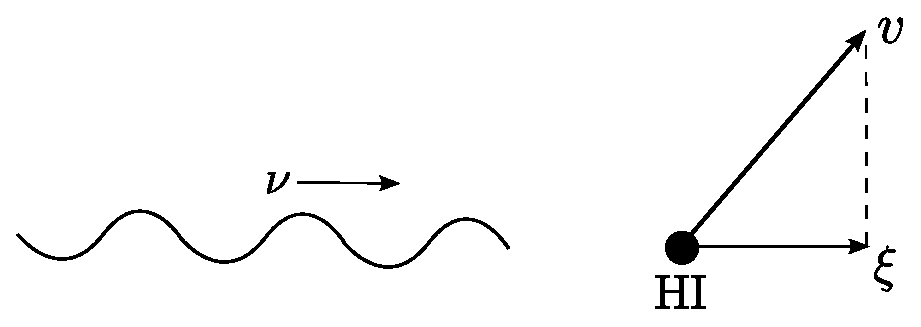
\includegraphics[width=8cm]{dopplerDiagram.eps}
  \caption{This diagram represents the process of Doppler broadening. The HI atom is moving away with velocity $v$ from incoming radiation with frequency $\nu$. The observed frequency of the radiation in the atom's rest frame is $\nu(1-\xi/c)$ where $\xi$ is the component of the velocity parallel with the incident radiation. }
  \label{fig:dopplerDiagram}
\end{figure}


where $T$ is the temperature of the gas, $\xi$ is the velocity and $k_{\text{B}}$ is the Boltzmann constant\gloss{$k_{\text{B}}$}{Boltzmann constant}Incident radiation will appear red/blueshifted in the frame of the absorbing atom with the shift being proportional to the atom's velocity \textit{parallel} to the incident radiation, as shown in Figure \ref{fig:dopplerDiagram}. Specifically, a photon with frequency $\nu$ will be observed by the atom to have frequency $\nu(1-\xi/c)$, where $\xi$ is the component of the atom's velocity \textit{away} from the incident radiation. Convolving our line profile with a Maxwell-Boltzmann distribution effectively involves replacing our expression in Eq. \ref{eq:IntroLineProfile} with

{\bf factors of $\lambda_{\alpha}??$}
\begin{align}
\sigma &\to \dfrac{\pi e^2}{m_e c}f_{\alpha}\lambda_{\alpha} \int_{-\infty}^{\infty} \dd \xi\ \phi(\nu(1-\xi/c)) W(\xi)\\
&= \dfrac{\pi e^2}{m_e c}f_{\alpha}\lambda_{\alpha} \int_{-\infty}^{\infty}\dd \xi\ \phi(\nu(1 - \xi/c)) \left(\pi \xi_{0}^{2} \right)^{-1/2} e^{-\xi^2/\xi_{0}^2} \\
&= \dfrac{\pi e^2}{m_e c} \frac{f_{\alpha}}{\pi} \left( \pi \xi_0^2 \right)^{-1/2} \int_{-\infty}^{\infty} \dd \xi \dfrac{(\Gamma/4\pi) e^{-\xi^2/\xi_{0}^{2}}}{(\nu-\nu_{0}(1-\xi/c))^2+(\Gamma/4\pi)^2}. \label{eq:IntroConvolution}
\end{align}

Here, we can make a couple substitutions and redefinitions:

\begin{align}
\Delta v_{\text{D}} &\equiv \nu_{0}\dfrac{\xi_{0}}{c} & y &\equiv -\xi/\xi_0 \\
v &\equiv \dfrac{\nu - \nu_{0}}{\Delta v_{\text{D}}} & a &\equiv \dfrac{\Gamma}{4\pi \Delta v_{\text{D}}}.
\end{align}

The quantity $\Delta v_{\text{D}}$ is known as the ``Doppler parameter" and is the red/blueshift in frequency space that the atom sees due to its thermal motion. The quantity $v$ is just the distance from line center in velocity space in units of the Doppler parameter. The quantity $a \equiv (\Gamma/4\pi)/\Delta v_{\text{D}}$ represents the ratio of the natural line width to the Doppler width. Rewriting our expression in Eq. \ref{eq:IntroConvolution}, we obtain

\begin{align}
\sigma(\nu) &= \dfrac{\pi e^2}{m_e c}f_{\alpha}\dfrac{1}{\sqrt{\pi}\Delta v_{\text{D}}} \dfrac{a}{\pi}\int_{-\infty}^{\infty}\dd y\ \dfrac{e^{-y^2}}{(v-y)^2+a^2}\\ 
&\equiv \dfrac{\sqrt{\pi} e^2}{m_e c} f_{\alpha}\dfrac{H(a,v)}{\Delta v_{\text{D}}}
\end{align}
where $H(a,v)$ is known as the Hjerting function \gloss{Hjerting Function}{Also known as the \textit{Voigt Function}, this function is commonly used in describing line profiles which incorporate Doppler broadening and the natural line width. This function is very relevant when studying the hydrogen damping wing.} or the Voigt function\gloss{Voigt Function}{Also known as the \textit{Hjerting Function}, this function is commonly used in describing line profiles which incorporate Doppler broadening and the natural line width. This function is very relevant when studying the hydrogen damping wing.}. So finally, we have obtained an expression for the \lya\ line profile incorporating the natural line width and Doppler broadening. Overall, the effect of the temperature acts to smear out the absorption line on scales of order $\sim 10\kms$ from line center. The greater the temperature, the larger the Doppler parameter and the greater the extent of the smearing. At scales $\gtrsim 100\kms$, the damping wing dominates the line profile. The profile is complex, but nonetheless, it encodes information about the underlying IGM temperature. Therefore, if simulations can generate accurate mock spectra for a variety of thermal histories, then comparisons between Voigt profile fits on the actual and mock spectra should be able to provide insight on the thermal properties of the IGM. 


This is the procedure undertaken by \cite{BoltonQuasar}. In Figure \ref{fig:QuasarProximityTemp}, they look for \lya\ absorption lines in the proximity zones of a high-redshift quasar in order to fit for the associated Doppler parameter and make inferences about the temperature. The top panel shows the fractional transmission for a mock quasar spectrum. The dashed curves indicate regions where absorption-line fitting was carried out and the vertical arrows indicate where the line centers were found from the fits. The second and third panel show the underlying temperature and density field, respectively. The bottom panel shows the true spectrum in question along with the same information regarding the line profile fits. These authors were able to use these fits to make inferences about the temperature of the IGM nearby the quasar. From these temperature measurements, and through comparison to mock spectra properties, these authors were able to place interesting limits on the ending of reionization ($z_{\text{H}} <  9$ assuming that the quasar reionizes its vicinity and Pop II stars drive reionization). This specific measurement is very difficult, however. The argument is essentially that the inferred temperature of the gas is too hot for reionization to have ended long before $z = 9$, otherwise the gas would have had more time to cool below the measured temperature. However, the regions nearby quasars should see a significantly-enhanced ionization field and all constraints made from measurements within this region hinge on ones ability to accurately account for such effects. 


The aforementioned technique for measuring the temperature is useful, but has the drawback that it requires the ability to detect \textit{individual absorption lines} in order to confidently fit a Voigt profile. However, at $z > 5$, it is no longer the case that absorption in the forest is due to isolated absorbers but is instead driven by density fluctuations in the diffuse IGM. As such, individual absorption features blend together and the forest becomes somewhat inverted where, instead of stretches of transmission being punctuated with absorption features, stretches of absorption are punctuated with transmission features. This renders the goal of fitting for individual Voigt profiles impossible in the IGM. This also explains why \cite{BoltonQuasar} analyze the IGM  nearby a high-redshift quasar, where the transmission is enhanced due to the strengthened ionization field. 


An alternative approach to fitting line profiles is to measure the small scale power of the flux fluctuations (e.g., \citealt{Lidz2010}, \citealt{Theuns2002a}, \citealt{zaldarriaga2002searching}). This involves applying a localized wavelet filter to measurements of the \lya\ forest in order to measure the level of small-scale fluctuations. As we mentioned, large temperatures will lead to a larger Doppler parameter which will smear out small-scale structure. Thus, a large response to a small-scale wavelet filter would indicate significant small-scale structure and suggest a lower temperature for the gas. This approach has the important advantage that it doesn't rely on individual absorption lines to be discernible in order to extract temperature measurements. In \S \ref{sec:IGMTemperature}, we show that this can be used to constrain the IGM temperature at $z > 5$, \textit{even in typical regions of the IGM}.

%% Maybe we can defer discussion of this equation to chapter 3?
%\begin{align}
%\dfrac{\dd T}{\dd t} &= -2HT + \dfrac{2T}{3(1+\delta)}\dfrac{\dd \delta}{\dd t} + \dfrac{T}{\mu} \dfrac{\dd \mu}{\dd t} + \dfrac{2\mu m_p}{3\rho k_B}(\mathcal{H} - \Lambda) \label{eq:dtdt}
%\end{align}

\begin{figure}[h]
  \centering
  \includegraphics[width=11cm]{BoltonIGMTemperature_Fig2.ps}
  \includegraphics[width=11cm]{BoltonIGMTemperature_Fig2b.ps}
  \caption{This figure shows mock spectra, and corresponding simulated IGM properties, from \cite{BoltonQuasar} in the top four panels. The bottom panel shows the observed spectrum from SDSS J0818+1722, which \cite{BoltonQuasar} use in order to make temperature measurements inside the proximity zone. Dashed lines indicate regions where Voigt-profile fitting was performed and downward arrows indicate the detected centers of the Voigt profiles. {\bf Maybe Bolton and Becker is better to use here? Larger sample of quasars, same basic idea...}}
  \label{fig:QuasarProximityTemp}
\end{figure}


\subsubsection{Motivation for this Work}

This discussion of the \lya\ forest as a tool for constraining the EoR highlights several of the current drawbacks of the approach. Among these, the largest is arguably the degeneracy between different sources of saturated absorption in the \lya\ forest. If one could find a way to determine if absorption in the \lya\ forest was certainly happening as a result of underlying neutral hydrogen, then it would be easier to interpret observations in terms of the overall neutral fraction of the Universe. We highlighted one example of how this has been done: the hydrogen damping wing redward of \lya. While a useful approach, this also suffers from drawbacks of its own, namely the limited number of high-redshift spectra suitable for damping-wing searches and the fact that regions surrounding quasars are not expected to be representative of the IGM as a whole. This helps motivate two approaches we consider in \S \ref{sec:NeutralIslands}. Namely, we identify the hydrogen damping wing and absorption due to deuterium as ``smoking gun" signals of underlying hydrogen and search for them in typical regions of the IGM. Obviously, it will become clear that this approach suffers from its own drawbacks but it does provide an independent measurement useful for constraining the ionization state of the high-redshift IGM.

Second, we have discussed some difficulty in making measurements of the temperature of the high-redshift IGM. Namely, due to the high levels of absorption in the \lya\ forest of quasar spectra at these redshifts, traditional methods of inferring the IGM temperature are inapplicable except in the highly-complex near-zones of quasars. This motivates the development of a temperature-measurement technique which is applicable to typical regions of the high-redshift IGM. Such a technique is proposed in {\bf cite} and discussed in \S \ref{sec:IGMTemperature}.


\subsection{The 21-cm Line}\label{sec:21cm}

The 21-cm line refers to the hyperfine splitting of the hydrogen atom where, due to the interaction between the magnetic dipole moments\gloss{Magnetic Dipole Moment}{The magnetic dipole moment of an object is related to the torque it would experience when placed in an external magnetic field. Magnetic moments are often relevant for bar magnets or loops of current. In the context of the hydrogen atom, the spin of the proton and electric render them as a sort of ``loop of current'' which gives them their own magnetic dipole moment.} of the electron and proton, a small energy difference exists between the configuration where the spins of the electron and proton are aligned versus where they are anti-aligned. The configuration where the spins are anti-aligned (and magnetic dipole moments are therefore aligned) is energetically favored and has a lower energy by $\Delta E \approx 6\times 10^{-6}$eV.\footnote{This is in contrast to a \lya\ photon which has energy $E \approx 10.2\text{eV}$, more than a million times greater.} Thus, spin-flip transitions will result in (from) the emission (absorption) of a photon with $\lambda \approx 21\cm$, $\nu \approx 1420\mhz$. This is shown schematically in Figure \ref{fig:21cmline}. 

%However, the 21-cm transition is a ``forbidden'' transition\gloss{Forbidden Transition}{This refers to atomic transitions which are not allowed under the quantum mechanical selection rules under the dipole approximation. Essentially, this means the transitions are relatively extremely rare compared to ``allowed'' transitions.}, meaning its rate of occurrence is extremely low. As a result,

As we discussed in \S \ref{sec:LyaForest}, the cross section or the \lya\ transition is extremely large, which presents us with a host of difficulties.  However, the Universe is essentially transparent to 21-cm photons, allowing them to travel unimpeded from distant neutral hydrogen to us. In principal, this allows us to observe the hydrogen density field directly up to redshifts of $z \sim 150$, \textit{far beyond the timescale of reionization} and far beyond the reach of the \lya\ forest. Measurements of the evolution of the 21-cm signal with redshift would allow us to construct something like a reionization ``movie'', which would constitute the ultimate constraint on reionization. 


Mapping the intensity of the 21-cm line during reionization avoids many other drawbacks of the \lya\ line as well. Namely, intensity mapping would provide us with a 3D volume of intensity values, as opposed to the \lya\ forest which is typically observed one sightline at a time. Also, since we are directly observing the hydrogen, interpretation of observations of the 21cm signal will be significantly simplified.

In this section, let us start with a overview of the physics of the 21-cm line and then continue by discussing a couple avenues by which the 21-cm signal could be utilized in order to constrain reionization. 


\subsubsection{The Intensity of the 21-cm Line}\label{sec:21cmPhysics}


Let us start by considering the brightness of 21-cm emission from a distant hydrogen gas cloud.\footnote{This discussion will closely follow \S 2.1 of \citealt{Furlanetto2006}, which is an excellent review of the 21-cm line.} This is usually described in terms of a \textit{specific intensity} and then in terms of a \textit{brightness temperature}\gloss{Brightness Temperature ($T_b(\nu)$)}{An object with a given specific intensity $I_{\nu}$ has a corresponding brightness temperature equal to the requisite temperature of a blackbody for its specific intensity to equal that of the object, $I_{\nu} = B_{\nu}(T_{b}(\nu))$.}\gloss{Specific Intensity ($I_{\nu}$)}{The specific intensity of light leaving a cloud of gas is the energy carried by the light per unit frequency, area, time, and solid angle.}. The specific intensity of light leaving our HI cloud is the amount of energy per unit frequency, time, area, and solid angle, denoted $I_{\nu}$. The brightness temperature is the required temperature of a blackbody to radiate with the same specific intensity at that frequency, i.e., $B_{\nu}(T_b) = I_{\nu}$, where $B_{\nu}$ denotes the blackbody spectrum. 


The light we observe from our HI cloud will be a combination of background light shining \textit{through} the cloud and light emitted by the cloud itself. This follows the radiative transfer equation (in the clouds frame)

\begin{align}
T_b(\nu) &= T_{\text{cloud}}(1-e^{-\tau_{\nu}}) + T_{\text{background}}e^{-\tau_{\nu}} \label{eq:cloudframe}
\end{align}
where the background light is from the CMB, such that $T_{\text{background}} = 2.73\text{K}(1+z)$, and $T_{\text{cloud}}$ is the \textit{spin temperature} of the cloud, defined below. The quantity $\tau_{\nu}$ is the frequency-dependent optical depth for absorption \textit{by} the HI cloud. This is equal to 

\begin{align}
\tau_{\nu} &= \int \dd s \sigma_{01}\left( 1 - e^{-E_{10}/k_{\text{B}}T_{\text{S}}} \right) \phi(\nu) n_{0} \label{eq:tau21}
\end{align}

where the integral is carried out along the line of sight through the cloud. In this expression, $E_{10} \approx 6\times 10^{-6}$eV is the energy of the transition, $\phi(\nu)$ is the line profile, $\sigma_{01}$ is the cross-section for 21-cm absorption by a hydrogen atom and $n_{0}$ is the number density of hydrogen atoms in the unexcited state. We follow the convention of \cite{Furlanetto2006} and denote the lower energy level by ``0'' and the higher energy level by ``1''. The ratio of the population of atoms in the excited state to the ground state is defined by the spin temperature and the degeneracy of the states:

\begin{align}
\dfrac{n_{1}}{n_{0}} &= \dfrac{g_1}{g_0}e^{-E_{10}/k_{\text{B}}T_{\text{S}}} = 3 e^{-E_{10}/k_{\text{B}}T_{\text{S}}}.
\end{align}

The excited state is the triplet state and has a three-fold degeneracy: $|\uparrow \uparrow \rangle$, $\dfrac{1}{\sqrt{2}}(|\uparrow \downarrow\rangle + |\downarrow \uparrow \rangle)$, $|\downarrow \downarrow\rangle$, and the lower-energy state is the singlet state: $\dfrac{1}{\sqrt{2}}( |\uparrow \downarrow\rangle - |\downarrow \uparrow \rangle)$, where arrows denote the spin. $T_{\text{S}}$ is the spin temperature and is defined via this equation. For our purposes, $T_{\text{S}} \gg E_{10}/k_{\text{B}}$, so we have $n_{1}/n_{0} = 3$ and

\begin{align}
1 - e^{-E_{10}/k_{\text{B}}T_{\text{S}}} &\approx \dfrac{E_{10}}{k_{\text{B}}T_{\text{S}}}.
\end{align}


 Furthermore, the integral along the line of sight of the number density of hydrogen atoms in the hyperfine ground state will simply be the column density of hydrogen atoms multiplied by 1/4, $N_{\text{HI}}/4$. Here, the factor of $\frac14$ accounts for the fact that only one out of four hydrogen atoms will be in the singlet state on average. Putting this together, Eq. \ref{eq:tau21} becomes
 
\begin{align}
\tau_{\nu} &\approx \sigma_{01} \dfrac{N_{\text{HI}}}{4} \dfrac{E_{\text{10}}}{k_{\text{B}}T_{\text{S}}} \phi(\nu)
\end{align}
where 
\begin{align}
\sigma_{01} &\equiv \dfrac{3c^2 A_{10}}{8\pi\nu^{2}}
\end{align}

is the cross section for 21-cm absorption and $A_{10} = 2.85 \times 10^{-15}\sec^{-1}$ is the spontaneous emission coefficient for the transition and $\phi(\nu)$ is the 21-cm line profile. As we discussed in \S \ref{sec:IntroIGMTemperature}, line profiles depend on several properties of the gas, however, here it is the case that Doppler broadening due to the expansion of the Universe dominates the line profile, such that

\begin{align}
\phi(\nu) \approx \dfrac{c}{s H(z) \nu}
\end{align}

where $s$ is the proper distance between two points expanding away from each other. Putting these pieces together, our expression for the optical depth becomes:

\begin{align}
\tau_{\nu} &\approx \dfrac{3c^2 A_{10}}{8\pi \nu^{2}} \dfrac{h \nu}{k_{\text{B}}T_{\text{S}}} \dfrac{c}{s H(z) \nu} \dfrac{n_{\text{HI}}\langle x_{\text{HI}}\rangle s}{4} \tag{$N_{\text{HI}} = s n_{\text{HI}}\axhi$}\\
&\approx \dfrac{3hc^3 A_{10}}{32\pi \nu^2 k_{\text{B}}T_{\text{S}}} \dfrac{n_{\text{HI}}\axhi}{H(z)}
\end{align}
plugging in values and evaluating at line center, \cite{Furlanetto2006} obtain

\begin{align}
\tau_{\nu_{0}} &\approx 0.0092 (1+\delta)(1+z)^{3/2}\dfrac{\axhi}{T_{\text{S}}}\left[ \dfrac{H(z)/(1+z)}{\dd v_{\parallel}/\dd r_{\parallel}} \right] 
\end{align}

where $\dd v_{\parallel}/\dd r_{\parallel}$ is the gradient in the line-of-sight velocity (peculiar velocity and velocity due to Hubble expansion) and the ratio of that with $H(z)/(1+z)$ represents the deviation from pure-Hubble expansion. For the purposes of the 21-cm probes we will discuss, we actually care about the \textit{contrast} between the 21-cm signal and the background CMB signal. Thus, the relevant brightness temperature contrast, in our frame, is 

\begin{align}
\delta T_{b} &= \dfrac{1}{1+z}\left[ T_{\text{S}}(1-e^{-\tau_{\nu_{0}}}) + T_{\text{CMB}}e^{-\tau_{\nu_{0}}} - T_{\text{CMB}} \right] \\
&= \dfrac{T_{\text{S}}-T_{\text{CMB}}}{1+z} (1 - e^{-\tau_{\nu_{0}}}) \\
&\approx \dfrac{T_{\text{S}}-T_{\text{CMB}}}{1+z} \tau_{\nu_{0}} \\ 
&\approx 9\text{mK}\cdot x_{\text{HI}}(1+\delta)(1+z)^{1/2}\left[ 1 - \dfrac{T_{\text{CMB}}}{T_{\text{S}}} \right] \left[ \dfrac{H(z)/(1+z)}{\dd v_{\parallel}/ \dd r_{\parallel}} \right] \\ 
&\approx 24 \text{mK}\cdot x_{\text{HI}}(1+\delta)\left(\frac{1+z}{7}\right)^{1/2}\left[ 1 - \dfrac{T_{\text{CMB}}}{T_{\text{S}}} \right] \left[ \dfrac{H(z)/(1+z)}{\dd v_{\parallel}/ \dd r_{\parallel}} \right]. \label{eq:dTb}
\end{align}

Thus, we see that a neutral parcel of hydrogen at mean density and $z = 6$ and $T_{\text{S}} \gg T_{\text{CMB}}$, the brightness temperature contrast is $\sim 24\text{mK}$. 


\begin{figure}[h]
  \centering
  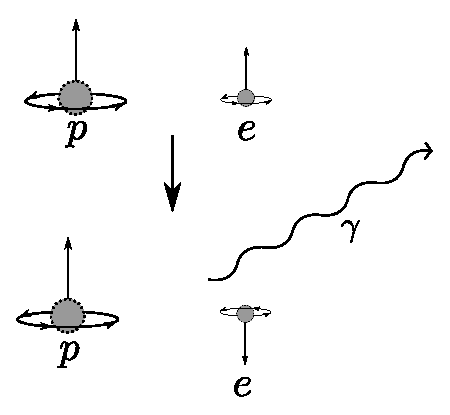
\includegraphics[width=8cm]{21cmline.eps}
  \caption{Schematic representation of the 21-cm transition where the transition between aligned spins of the proton and electron to anti-aligned spins results in the emission of a photon with $\lambda \approx 21$cm. }
  \label{fig:21cmline}
\end{figure}

\begin{figure}[h]
  \centering
  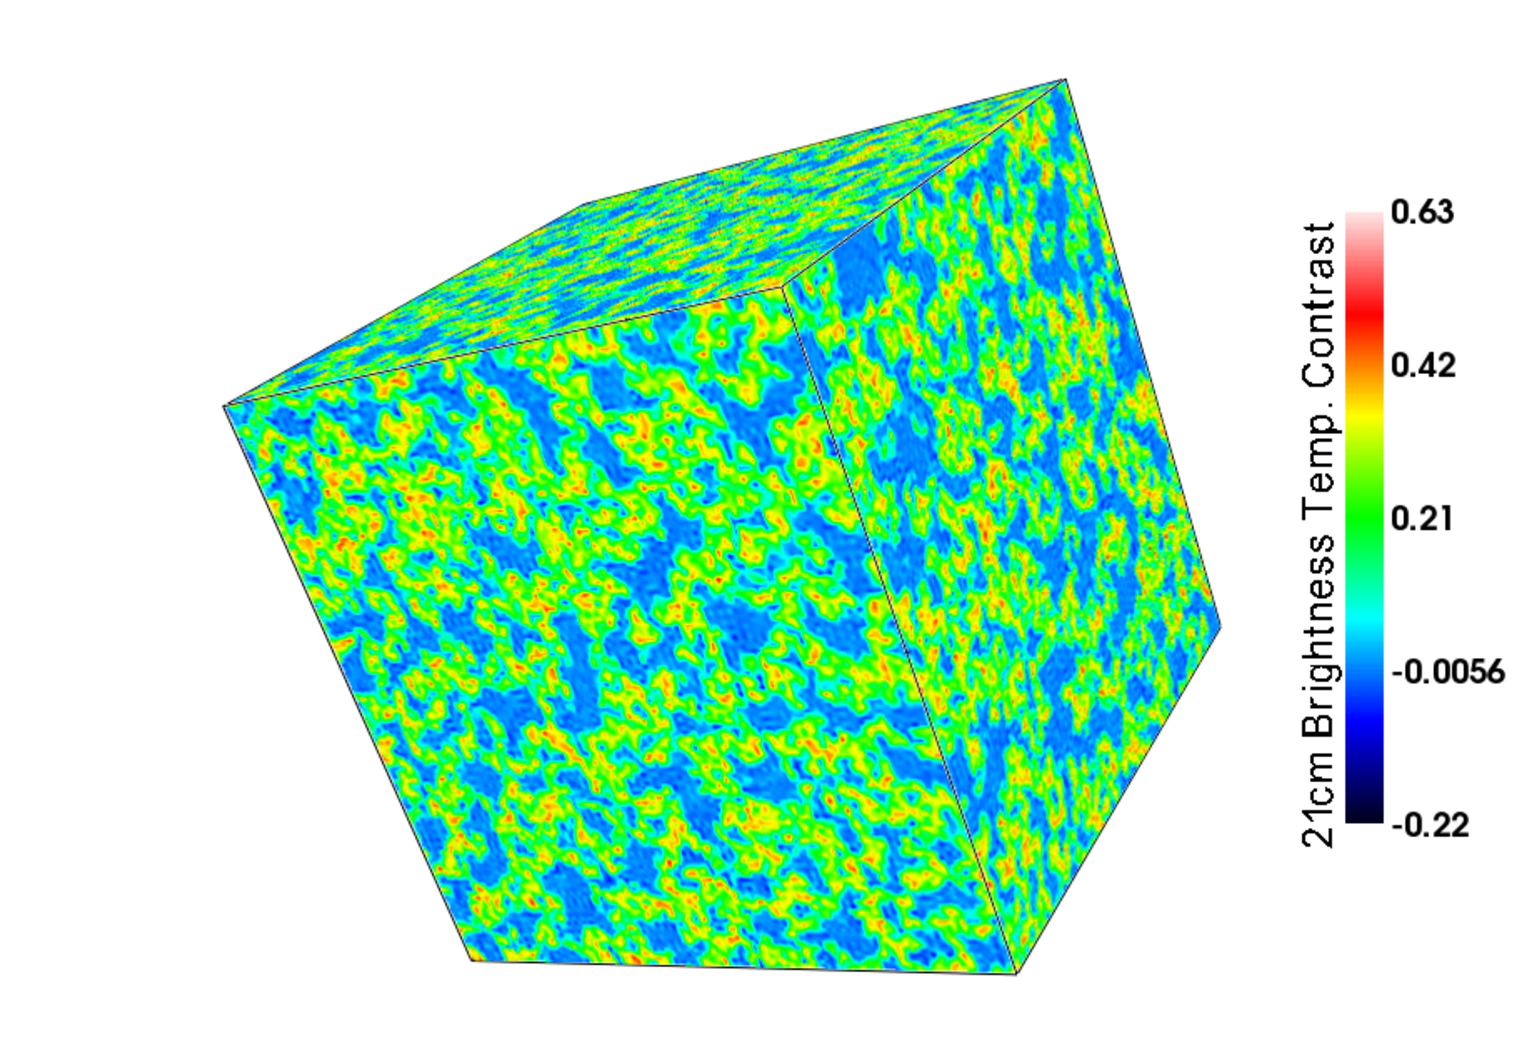
\includegraphics[width=8cm]{TalkSignal.eps}
  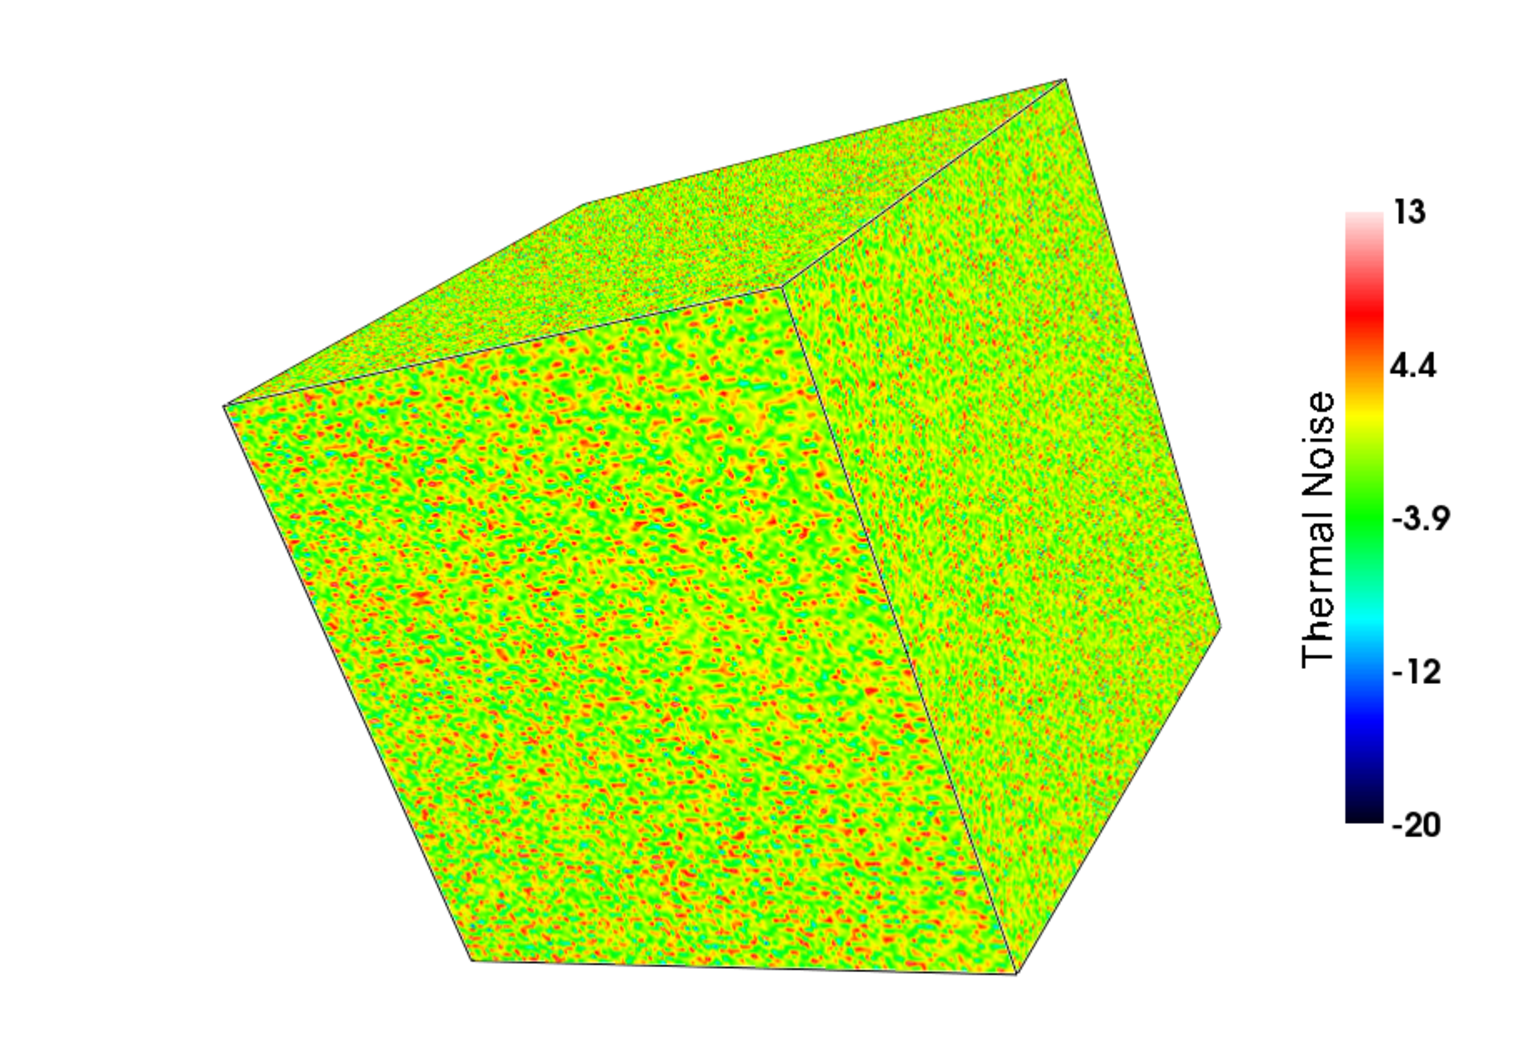
\includegraphics[width=8cm]{TalkNoise.eps}
  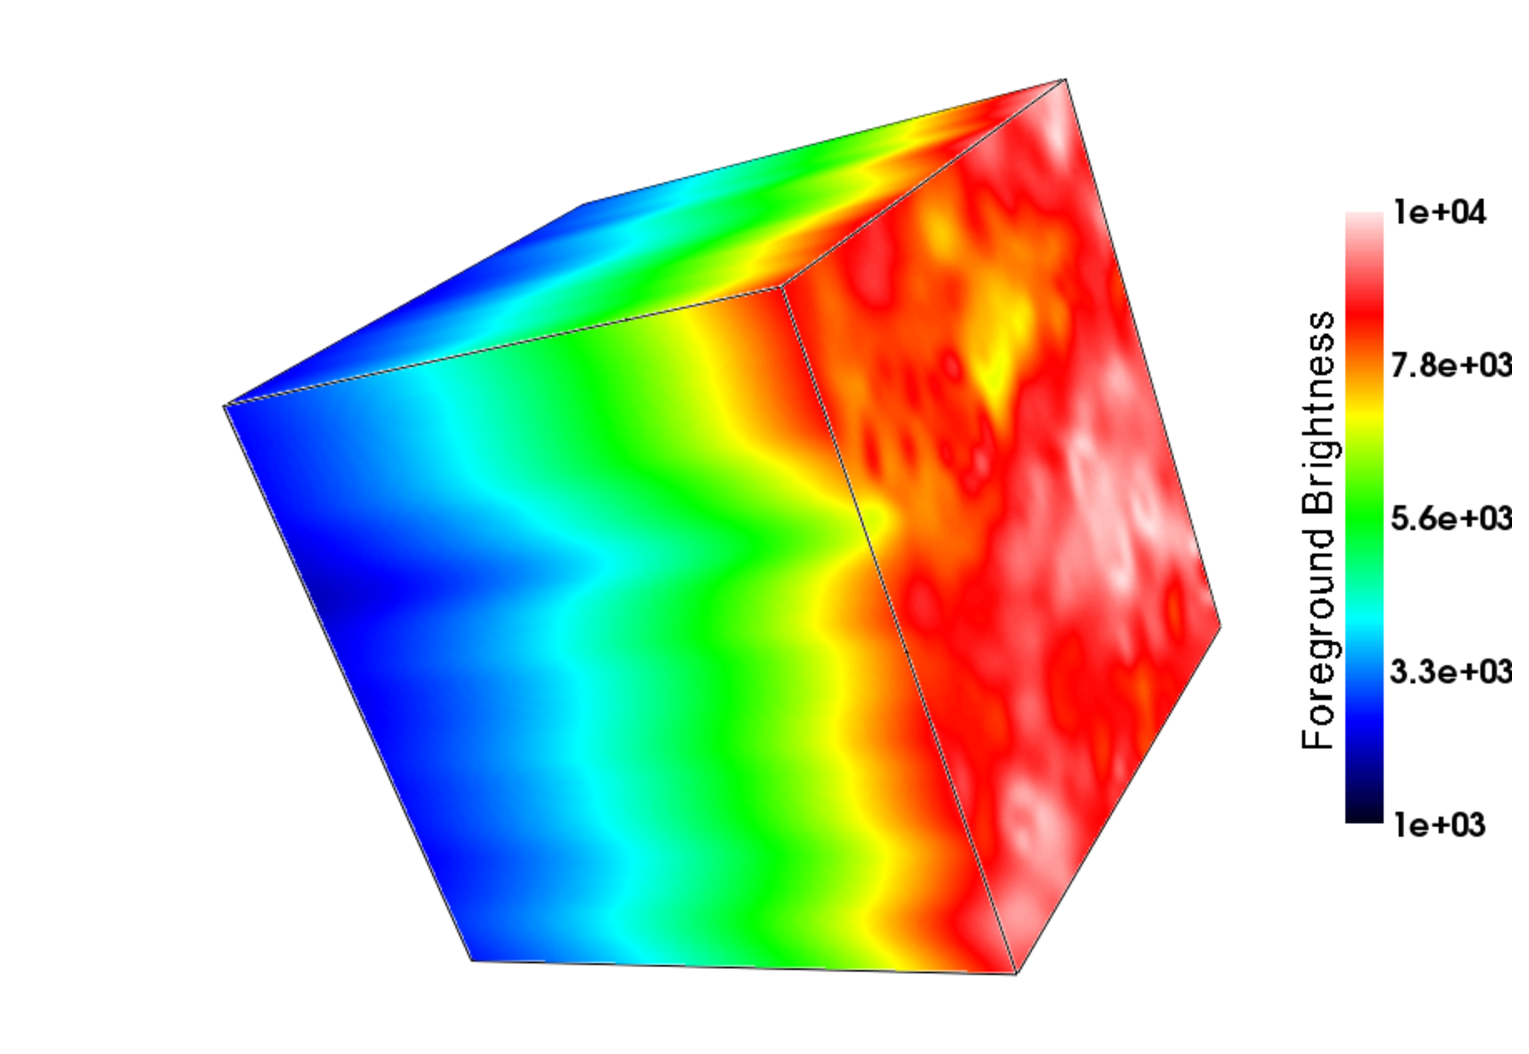
\includegraphics[width=8cm]{TalkFG.eps}
  \caption{Simulation cube of the 21-cm signal during reionization (top) along with simulated noise for an interferometer (middle) and the galactic foregrounds (bottom). This figure demonstrates that, while the sources of noise are several orders of magnitude larger than the signal, these three contributions to observations are dominant of different scales. The volume of each cube is 1 $(\text{Gpc}/h)^{3}$. In this figure, the line of sight direction away from the observer is to the right and slightly out of the page. }
  \label{fig:21cmCube}
\end{figure}


\subsubsection{21-cm Fluctuations with Interferometers} 


The first approach for utilizing the 21-cm line in order to learn about reionization that we will discuss is through the use of 21-cm fluctuations. The ultimate goal for the 21-cm line for people interested in reionization is to image the 21-cm intensity field for the duration of reionization. Since the 21-cm radiation of interest is emitted at $z \approx 10$, by the time it arrives to us, its wavelength will have redshifted to $\sim 2\meter$. Thus, observations of 21-cm fluctuations must be made with large interferometers, consisting of tens to thousands of antennae, and maximum separations (baselines) of the order 1 km. 

Before continuing, it may be helpful to provide a brief description of what interferometry is, for which we will follow \cite{morales2009reionization}. Interferometers are built of many antennae which observe the electric field at their location and correlate those measurements to image the sky. Let us consider a single antenna which observes a time-and-angle-dependent electric field, defined $E(\theta,t)$. A nearby antenna, separated from the first by the vector $\vec{r}$, will observe a similar electric field, but the field will have a phase shift owing to the difference in path length that the radiation had to travel between going to the first and the second antennae. If we are observing directly overhead, then light will have to travel an equal distance to reach either antenna. Conversely, if we are observing at the horizon along the line connecting the antennae, then it will take light extra time to reach one of the antenna opposed to the other ($\Delta t = |\vec{r}|/c$). This is illustrated in Figure \ref{fig:interferometry}. Based on this figure, we can see that the extra path length for the light will be 

\begin{align}
\Delta \ell &= \vec{r}\cdot\hat{\theta}
\end{align}

resulting in a \textit{phase difference} of 

\begin{align}
\Delta \phi &= 2\pi \frac{\vec{r}\cdot\hat{\theta}}{\lambda}.
\end{align}


Therefore, if the first antenna sees an electric field $E(\theta,t)$, then the second antenna will see $E_2(\theta,t) = E(\theta,t)e^{-2\pi i (\vec{r}\cdot{\theta}/\lambda)}$. Therefore, the observed electric field at any position, $\vec{r}$, is related to that at the first antenna by

\begin{align}
E(\vec{r},\theta,t) &= E(\theta,t)e^{-2\pi i (\vec{r} \cdot \hat{\theta}/\lambda)}.
\end{align}

If we integrate over the entire sky, we find

\begin{align}
E(\vec{r},t) &= \int \dd^{2} \theta E(\theta,t) e^{-2\pi i (\vec{r}\cdot \hat{\theta}/\lambda)}.
\end{align}

However, the expression on the right appears very familiar to us since it is simply a Fourier transform. Therefore, we see that the observed electric field on the surface of the Earth is actually just a Fourier transform\gloss{Fourier Transform}{A Fourier transform essentially describes a function as a weighted sum of infinitely many sine waves with different frequencies. The Fourier transform describes the weights of the different sine curves and therefore gives information about the relevant distances scales in your function.} of the electric field on the surface of the sky. This is basically what allows measurements at many locations on the ground to be converted into measurements of the 21-cm signal across the sky. Furthermore, each pair of antenna essentially measure a particular Fourier \textit{mode}, $k$, on the sky:

\begin{align}
{\bf k} &= \frac{2\pi {\bf u}}{D}
\end{align}

where ${\bf u}$ denotes the separation of a pair of antenna in units of the observed wavelength, $D$ is the co-moving distance to the source of the emission, and ${\bf k}$ is akin to a spatial frequency at the location of the emission. Thus, this demonstrates that many measurements on the ground can give us information of the 21-cm signal as a function of position on the sky, with widely-separated antenna providing information on \textit{small scales} and closely-separated antenna providing information on the large scales. Several experiments are currently planned or underway with the goal of measuring this signal. These include the Precision Array for Probing the Epoch of Reionization (PAPER, \citealt{Parsons2012}, underway), the Murchison Widefield Array (MWA, \citealt{Tingay2012}, underway), the Hydrogen Epoch of Reionization Array (HERA\footnote{{\tt http://reionization.org/}}, planned), the Square Kilometer Array (SKA\footnote{{\tt https://www.skatelescope.org/}}, scheduled construction 2018), the Low Frequency Array (LOFAR, \citealt{2013A&A...550A.136Y}, underway), and the Giant Metrewave Radio Telescope (GMRT, \citealt{Paciga2011}, underway).


However, before these experiments can uncover the cosmological 21-cm signal, they must first overcome several formidable sources of noise. Synchrotron emission\gloss{Synchrotron Radiation}{Radiation emitted by charged particles undergoing radial acceleration, such as in synchrotron particle accelerators. This constitutes a significant source of noise for 21-cm observations.}, free-free emission\gloss{Free-Free Emission}{Emission from a charged particle that is free both before and after the interaction. Examples include electrons in an ionized hydrogen cloud interacting with protons without being captured.}, and Bremsstrahlung radiation\gloss{Bremsstrahlung Radiation}{Emission from charged particles undergoing acceleration due to interactions with other charged particles. Literally translates to ``braking radiation''.} from our own galaxy constitute the largest nuisance at the frequencies of interest ($\nu \approx 140\mhz$) in sheer magnitude. In a relatively ``cold'' spot on the sky, \cite{Furlanetto2006} state that the intensity of this radiation obeys the following scaling relation:

\begin{align}
T_{\text{sky}} \sim 180 \left( \dfrac{\nu}{180\mhz} \right)^{-2.6}\kelvin, \label{eq:Tsky}
\end{align}

which scales to $T_{\text{sky}} \sim 130\kelvin$ at $z = 6$. Thus, we see in this specific example, the intensity of the foreground emission from our galaxy should be $\gtrsim 5000$ times greater than the 21-cm signal itself. Furthermore, while it is often the case that sources of noise can be beaten down with increased observation time, these galactic foregrounds are a permanent feature of the sky.  While this presents an enormous challenge for observing the 21-cm signal from the EoR, not all hope is lost. 


We can see from Eq. \ref{eq:Tsky} that the foreground noise from the galaxy should vary very \textit{smoothly} with frequency. Meanwhile, for the 21-cm signal, slight decreases in observed frequency are equivalent to observing the 21-cm signal from a more distant point in space. For example, in the case of ionized bubbles of size $\ell \approx 10\mpch$, we would expect fluctuations of 100\% in the 21-cm signal over this distance. However, this distance at a redshift of $z \approx 7$ corresponds to a frequency change of $\Delta \nu \approx 1\mhz$ and a  (relatively predictable) change in the amplitude of the foreground signal of only $\lesssim3\%$. This is further demonstrated by Figure \ref{fig:21cmCube}. The top cube shows what the 21-cm signal would look (in arbitrary units) like for a 1Gpc/$h$ cube of the Universe from a reionization simulation. We can see bubbles of size $\sim10\mpch$ and therefore fluctuations in the 21-cm signal on that scale. In the bottom panel, we show a simulation of the galactic foregrounds (provided by Piyanat Kittiwisit at ASU) corresponding to the same physical region in space. In this case, the dimension of the cube that goes to the right and slightly out of the page is the line of sight direction away from us. We see that, along this direction, the foreground emission varies very smoothly, as expected from Eq. \ref{eq:Tsky}. Thus, in principle, the contributions to the observed signal from the EoR and from the galaxy should separable. This is essentially done by removing large-scale modes from the observed signal, as briefly discussed in \S \ref{sec:Bubbleforegrounds}.



\begin{figure}[h]
  \centering
  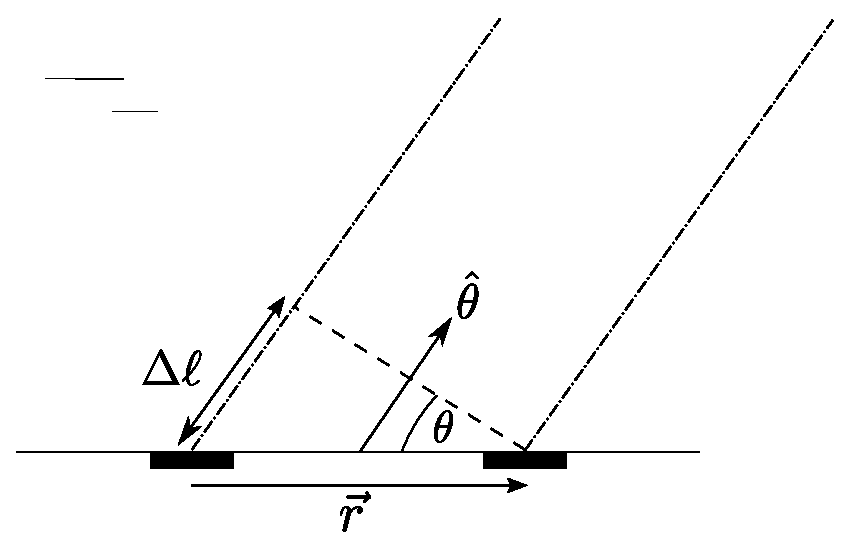
\includegraphics[width=8cm]{interferometry.eps}
  \caption{This figure depicts the extra path length, $\Delta \ell$, of radiation (dot-dashed lines) incident on two elements (solid black rectangles) in an array separated by $\vec{r}$ when considering a position on the sky $\hat{\theta}$.}
  \label{fig:interferometry}
\end{figure}


A second significant source of noise is thermal noise from the experiment itself. This is discussed in more detail in \S \ref{sec:Bubblenoise}, but the power spectrum for the noise should follow (\citealt{McQuinn2006},\citealt{Furlanetto2006})

\begin{align}
P_{\text{N}} &= \dfrac{T_{\text{sky}}^{2}}{B\ t_{\text{int}}} \dfrac{D^{2}\Delta D}{n(k_{\perp})}\left( \dfrac{\lambda^{2}}{A_{\text{e}}} \right)^{2}.
\end{align}

Here, $k_{\perp}$ is the component of ${\bf k}$ transverse to the line of sight, $B$ is the bandwidth of the observation, $t_{\text{int}}$ is the integration time for the experiment, $n(k_{\perp})$ is the number density of baselines observing the specific wavemode, $\Delta D$ is the depth of the observation field, and $A_{\text{e}}$ is the effective collecting area per tile. With the exception of $T_{\text{sky}}$ and $\lambda$ and $D$, these are controllable parameters of the experiment. This allows for several avenues toward beating down the thermal noise, the most popular of which are through increasing observation time, re-arranging tiles in order to alter $n(k_{\perp})$, and increasing collecting area. Thus, unlike the galactic foregrounds, the thermal noise is a nuisance which will become less and less important as experiments evolve. 


For the first generation of experiments, however, the levels of thermal noise should prevent the 21-cm signal from being mapped and prevent any reionization ``movies'' from being made. This is discussed in \cite{McQuinn2006} and shown in Figure \ref{fig:McQuinnSNR}. Specifically, this figure shows the fraction of pixels at each $k$ which will be imaged (have $\text{SNR} \geq 1$) for MWA (dashed), LOFAR (dot-dashed), and SKA (solid) assuming galactic foregrounds can be subtracted. With regard to foregrounds, though, it is likely that any $k$ modes below the vertical hatched line will be inaccessible due to residuals from the foreground subtraction. This demonstrates that, due to thermal noise, first-generation interferometers like the MWA and LOFAR will image a small fraction of the pixels at the $k$ modes unspoiled by foregrounds and will therefore be unable to make maps of the 21-cm sky during reionization.\footnote{This estimate is done assuming that fluctuations in the 21-cm signal are caused by density fluctuations rather than by fluctuations in the ionization field. The latter should lead to a larger signal and so, in this sense, this estimate is somewhat pessimistic. The general point still holds, however.} 

\begin{figure}[h]
  \centering
  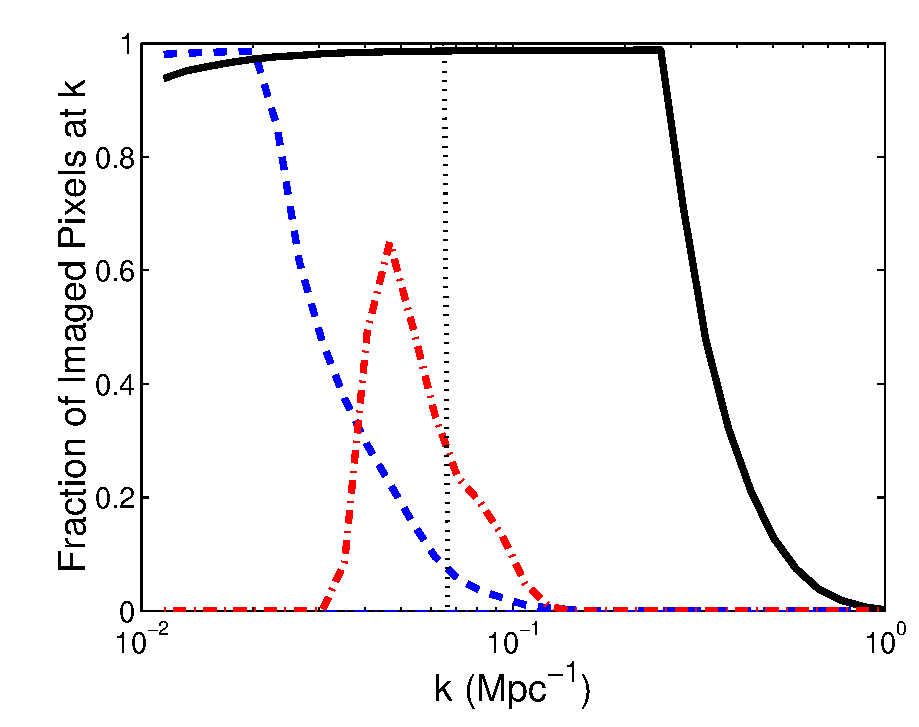
\includegraphics[width=8cm]{McQuinnSNR.eps}
  \caption{This figure shows the percentage of pixels ``imaged'' ($\text{SNR} > 1$) as a function of wavemode, $k$ for the MWA (dashed), LOFAR (dot-dashed), and the SKA (solid). The vertical hatched line shows the distance scale above with (smaller $k$) the residuals from foreground subtraction are expected to dominate the 21-cm signal. This demonstrates that, for first-generation 21-cm experiments, a very small fraction of pixels with $k > k_{\text{hatched}}$ will be ``imaged''. This estimate assumes that fluctuations in the 21-cm signal are driven from density fluctuations rather than fluctuations in the ionization field, so it is somewhat conservative. Taken from \cite{McQuinn2006}. }
  \label{fig:McQuinnSNR}
\end{figure}


In Figure \ref{fig:21cmCube} we show a random, qualitatively-representative simulated realization of thermal noise. While this panel indeed does demonstrate that thermal noise should dominate the 21-cm signal (top) in sheer magnitude, it also demonstrates that the fluctuations in the thermal noise are expected to happen on scales \textit{smaller} than those in the 21-cm signal. While galactic foregrounds ruin large-scale modes, and thermal noise ruin small-scale modes, an intermediate region of $k$-space should remain accessible to the interferometers. It will not be the case that first-generation interferometers can image or make movies of the 21-cm signal, but they still may learn about how the signal behaves on different physical scales, i.e. the \textit{power spectrum}, and how that behavior evolves with redshift. 


In fact, \cite{Lidz2008} investigate the evolution of the power spectrum throughout reionization under several simulated reionization scenarios. They find that a generic result to all the models is that the \textit{slope} of the power spectrum, in the accessible $k$-mode range ($0.1\ h/\text{Mpc} \leq k \leq 1\ h/\text{Mpc}$) should \textit{decrease} as reionization evolves. Meanwhile, the \textit{amplitude} of the power spectrum in this $k$-mode range should rise until reionization reaches its midpoint and then fall. Thus, measuring the 21-cm power spectrum at several redshifts and confirming this behavior can, first, increase our confidence that we are in fact observing the 21-cm signal from reionization and, second, help us learn about the reionization process itself. 

\begin{figure}[h]
  \centering
  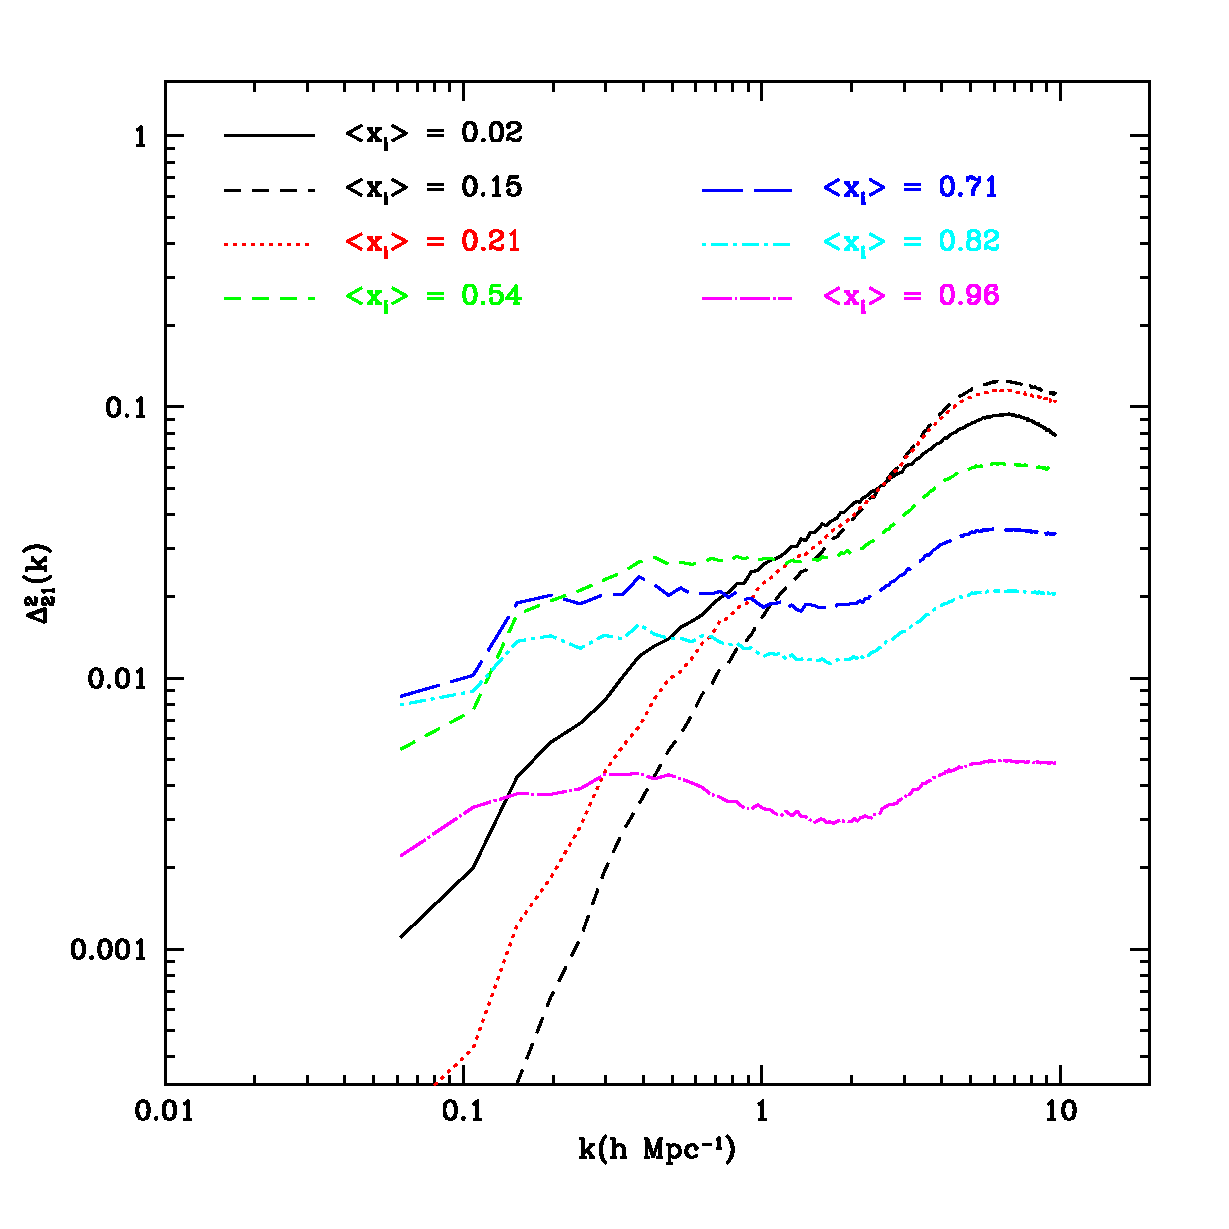
\includegraphics[width=7cm]{LidzPSEvolution.eps}
  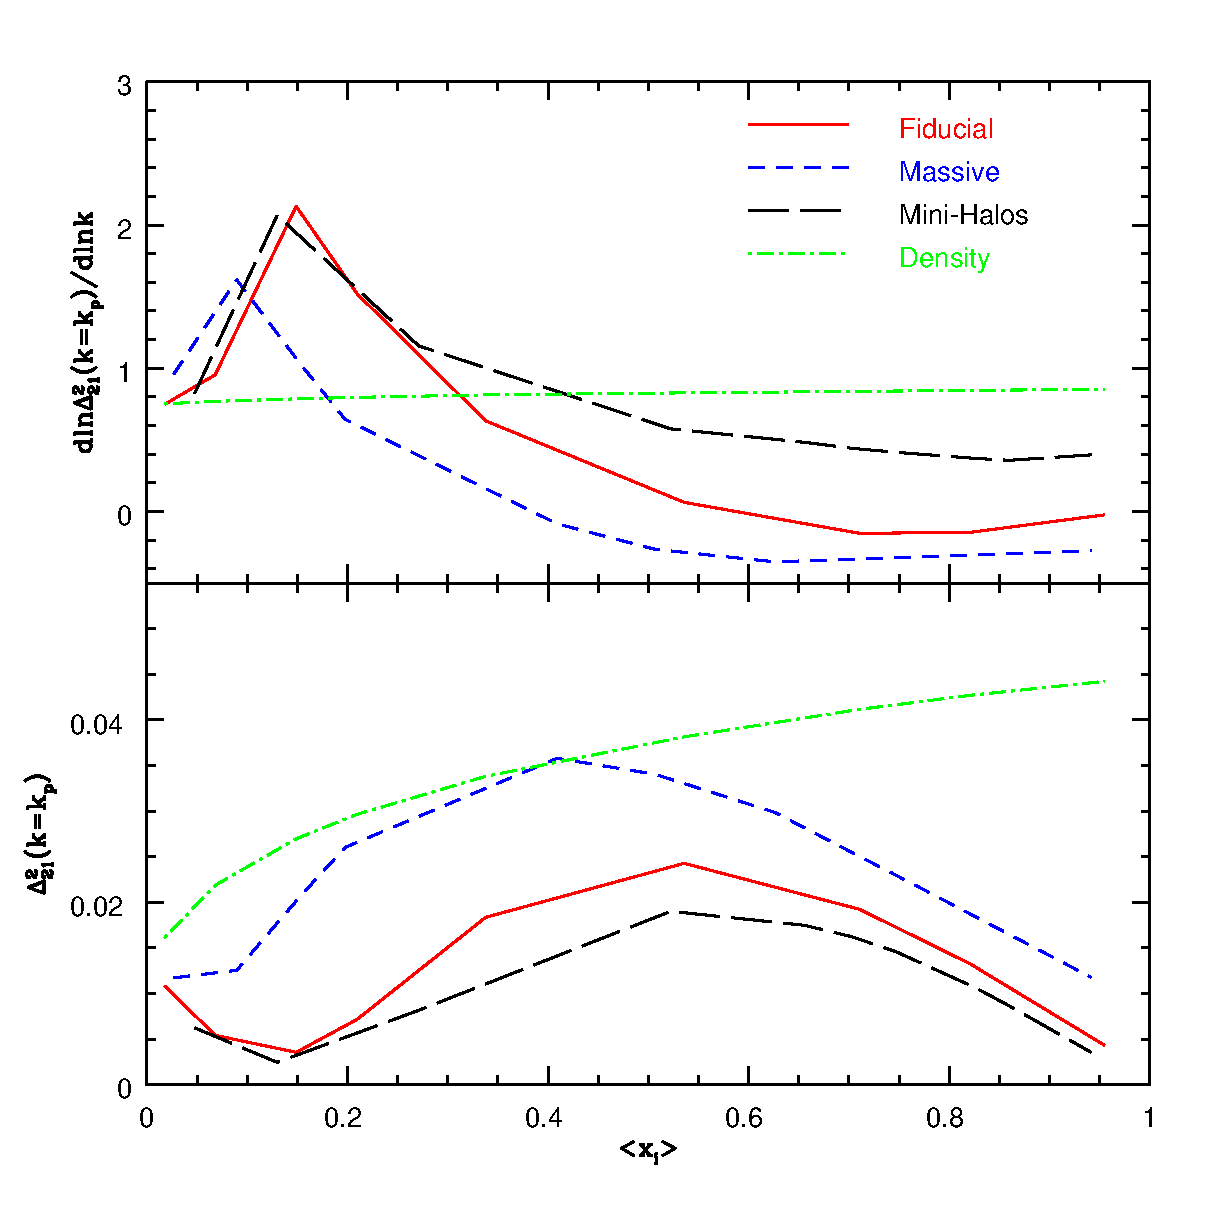
\includegraphics[width=7cm]{LidzSlopeAndAmpEvolution.eps}
  \caption{The left panel shows the evolution of the power spectrum during reionization for the fiducial reionization model in \cite{Lidz2008}. We can see that, as reionization progresses, the slope of the power spectrum in the $k$-mode range accessible to interferometers ($0.1\ h/\text{Mpc} \leq k \leq 1\ h/\text{Mpc}$) declines. The \textit{amplitude} of this part of the power spectrum peaks around $\axhi = 0.5$. The right-hand panel shows the evolution of the power spectrum slope (top) and magnitude (bottom) during reionization for a few different reionization models. This demonstrates that the general power-spectrum evolution described is generic to many reionization models. Both figures are taken from \cite{Lidz2008}.}
  \label{fig:todo}
\end{figure}


Constraints have already been placed on the nature of the EoR using this approach by, for example, the PAPER collaboration. In \cite{ali2015paper} and \cite{pober2015paper}, upper limits on the amplitude of the 21-cm power spectrum at $z = 8.4$ are converted to constraints on the IGM properties. Specifically, we see in Eq. \ref{eq:dTb} that, if $T_{\text{S}} \ll T_{\text{CMB}}$, then the amplitude of the 21-cm signal can become arbitrarily large. As we will touch on in \S \ref{sec:Global21cm}, for redshifts relevant to reionization, the spin temperature is tied to the gas temperature. As such, upper limits on the 21-cm power spectrum amplitude can be converted to lower limits on the spin temperature and therefore also lower limits on the gas temperature. These authors use the upper limits to rule out a very cold reionization scenario. 


Measurements of the 21-cm power spectrum and its evolution are powerful probes of the Epoch of Reionization, but they are inherently indirect. Making detailed maps of the 21-cm radiation field would be much more direct, but will likely be out of reach for first and second generation experiments. However, the presence of an intermediate range in $k$ space which remains relatively un-spoiled by noise could provide us with the ability to make \textit{crude} maps of the 21-cm field and/or directly image individual large ionized regions. Direct observations of individual ionized regions would provide unambiguous evidence that reionization is ongoing and could also provide hints as to the sources of the ionizing photons and the volume-averaged neutral fraction. Such proposed approaches generally attempt to reconstruct the underlying signal by downweighting the $k$ modes of the observed signal which are expected to be dominated by noise. While these techniques are out of reach for first-generation experiments like PAPER, they may very well be suitable for successor experiments, such as HERA. We develop some of these filtering approaches in \S \ref{sec:Bubble} and explore their utility for a variety of plausible experiments.


\subsubsection{The Global 21-cm Signal}\label{sec:Global21cm}

An alternative method of extracting information from the 21-cm line is to use the \textit{sky-averaged} 21-cm signal. In the previous section, we discussed the difficulties faced in obtaining the necessary resolution to map out fluctuations in the 21-cm radiation field. However, Equation \ref{eq:dTb} is rich with astrophysical information on its own without even considering spatial fluctuations. Therefore, natural questions to ask would be if it is easier to simply measure the average signal rather than map the fluctuations and what astrophysical information can be obtained in that way? For convenience, the brightness temperature contrast for the 21-cm signal from \S \ref{sec:21cmPhysics} is:

\begin{align}
\delta T_{b} &\approx 24 \text{mK}\cdot x_{\text{HI}}(1+\delta)\left(\frac{1+z}{7}\right)^{1/2}\left[ 1 - \dfrac{T_{\text{CMB}}}{T_{\text{S}}} \right] \left[ \dfrac{H(z)/(1+z)}{\dd v_{\parallel}/ \dd r_{\parallel}} \right].
\end{align}

As mentioned earlier, for the end of reionization, the dependence on the spin temperature drops out. The result is that the amplitude of a sky-averaged signal  would be most sensitive to the neutral faction, with ionized regions emitting no 21-cm signal. Thus, one could imagine plotting the sky-averaged 21-cm signal against redshift and observing a shrinking signal coinciding with the EoR. 


However, the utility of the global 21-cm signal is not limited to the Epoch of Reionization. Specifically, prior to reionization, $\axhi$ will be fixed at 1 and the spin temperature is expected to drop to the point where $1 - T_{\text{CMB}}/T_{\text{S}} \not\approx 1$. This is interesting because the spin temperature itself depends on several astrophysical processes. A very high-level description of this is shown in Figure \ref{fig:TsEvolution}.\footnote{This figure and much of the following discussion is taken from notes from Adam Lidz's ``Topics in Cosmology'' class, taught in the Fall of 2011.} The precise evolution of the spin temperature is not well known, but a reasonable approximate description could be as follows:

\begin{enumerate}
\item [] \underline{$z > 150$:} Collisions within the gas are frequent enough to fix the spin temperature to the gas temperature, $T_{\text{S}} = T_{\text{K}}$. However, the gas temperature is equal to the CMB temperature, so the 21-cm signal is \textit{unobservable}.
\item [] \underline{$30 < z < 150$:} Collisions are efficient at coupling the gas temperature to the spin temperature. Furthermore, the gas cools to below the CMB temperature, making the 21-cm signal \textit{obervable}. 
\item [] \underline{$20 < z < 30$:} The gas density drops enough so that collisions are not efficient at coupling the spin temperature to the gas temperature. As a result, the spin temperature approaches the CMB temperature and the 21-cm signal is \textit{unobservable}. 
\item [] \underline{$15 < z < 20:$} Wouthuysen field effect re-couples the spin temperature to the gas temperature, which is still below the CMB temperature. This renders the 21-cm signal \textit{observable in absorption}. 
\item [] \underline{$ z < 15:$} The first X-ray sources form and heat the gas well above the CMB temperature. As a result, the 21-cm signal becomes \textit{observable in emission}.
\item [] \underline{$ z \lesssim 5.5:$} The completion of reionization effectively eliminates the 21-cm signal from the IGM all together. The 21-cm signal is still observable in pockets of neutral gas surrounding galaxies. 
\end{enumerate}


\begin{figure}[h]
  \centering
  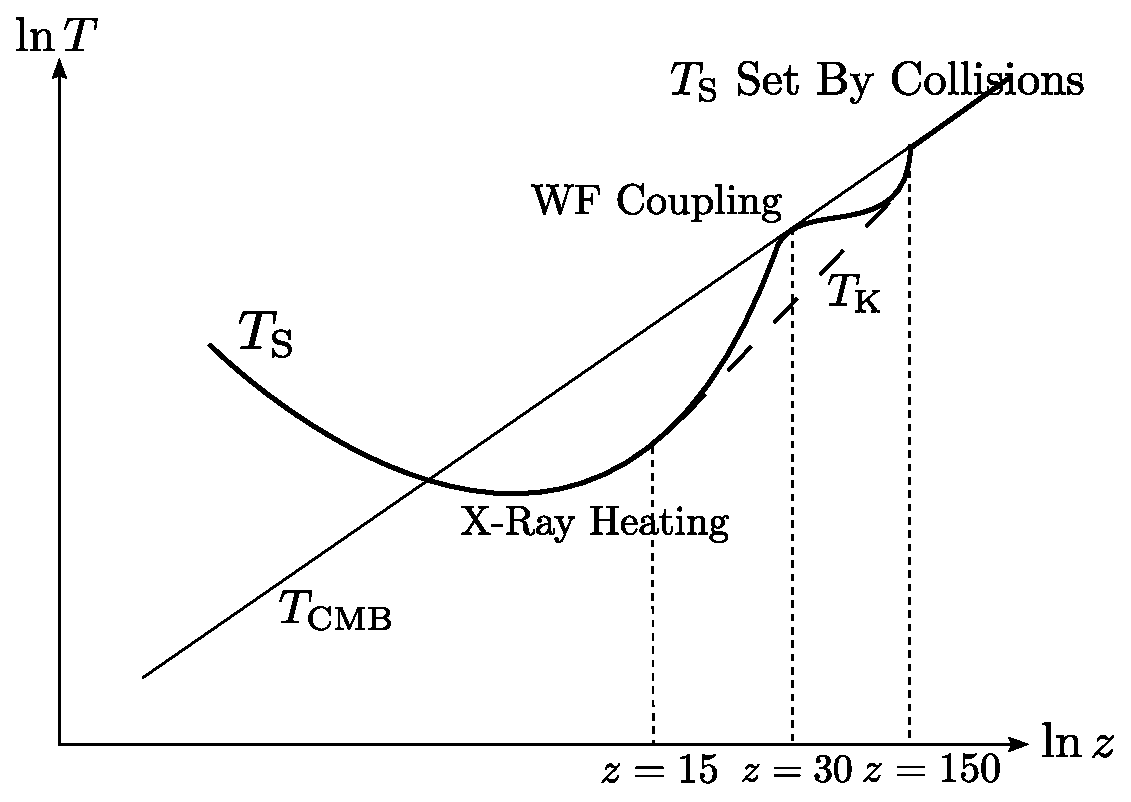
\includegraphics[width=12cm]{TsEvolution.eps}
  \caption{Schematic representation of a plausible $T_{\text{S}}$ signal including a few landmarks. This is adapted from notes taken in the course ``Topics in Cosmology''.}
  \label{fig:TsEvolution}
\end{figure}



\subsection{The Cosmic Microwave Background}\label{sec:CMB}


The Cosmic Microwave Background (CMB) is the earliest accessible picture we have of the Universe. It is composed of photons which have travelled, largely uninterrupted, from when the Universe was $\sim380,000$ years old\footnote{This is $\sim3\times 10^{-3}\%$ of its current age. If the Universe were an 80-year-old human, then the CMB would provide a picture of him/her when they were less than a day old.} to us today. Before this time, the Universe was hot enough that collisions between its constituent parts prevented the formation of neutral atoms (mostly hydrogen and helium). As a result, photons had an extremely short mean free path between collisions with free electrons. This makes this period of time completely opaque and impenetrable by observations. However, at $\sim380,000$ years, the Universe cooled to the point where neutral hydrogen could form (neutral helium having formed slightly earlier) and capture almost all of the remaining free electrons. Without a substantial number of free electrons, the mean free path of photons increased to the point where they could reach us today. Because of this, this CMB is also referred to as the ``surface of last-scattering''.


Therefore, the CMB is essentially a picture of the Universe at the time when photons decoupled from matter. As a result, it provides us with a picture of the matter distribution at this time and its value to cosmology cannot be overstated. While this is wonderful, in this thesis we are interested in the evolution of the Universe when it was $\sim500$ million years old, not $\sim380,000$, so how can the CMB help us? 


Well, similarly to how bright light from distant quasars/GRBs can give us information on the intervening gas, light from the CMB can do the same. While $\gtrsim90\%$ of photons will travel from the surface of last scattering to us without interacting, the other $\lesssim10\%$ of the photons will scatter off of free electrons that have been released as a result of reionization. Therefore, an interesting question is if this level of interaction can create an observable imprint in the CMB itself. In this section, we briefly discuss two such methods for searching for these imprints and their progress toward constraining the EoR.


\subsubsection{Thompson Scattering Optical Depth, $\tau_{e}$}


The first observable that we discuss is the CMB optical depth to Thompson scattering. As mentioned earlier, after the time of the surface of last-scattering, the density of free electrons drops low enough to allow photons to travel unimpeded. However, once reionization is underway, free electrons will be introduced into the IGM and will scatter a significant number of the CMB photons. The precise fraction of CMB photons that scatter in this way depends on the integrated electron density along the line of sight to the CMB. This is sensitive to the timing of reionization since CMB photons will have the opportunity to scatter off of electrons over a larger path length if reionization happens earlier. The percentage of CMB photons which scatter in this way is quantified through the Thompson scattering optical depth, $\tau_{e}$, where

\begin{align}
f_{\text{scattered}} &\approx 1-e^{-\tau_{e}} \approx \tau_{e}
\end{align}

for small $\tau_{e}$. This is related to the density of electrons along the line of sight via\footnote{We have neglected the contribution to $n_e$ from singly-ionized helium in this expression for simplicity.}

\begin{align}
\tau_{e} &= \int \dfrac{\dd z\ c}{(1+z)H(z)}n_{e}(z)\sigma_{\text{Thom}}\\
&\approx \int \dfrac{\dd z\ c}{(1+z)H(z)} \bar{n}_{\text{H}}(z)(1 - \langle x_{\text{HI}}(z)\rangle) \sigma_{\text{Thom}}
\end{align}

where 

\begin{align}
\sigma_{\text{Thom}} &= \dfrac{8\pi}{3}\left(\dfrac{\alpha \hbar}{m_ec}\right)^2 \approx 6.65\times 10^{-25}\cm^{2}
\end{align}

is the frequency-independent cross section for Thompson scattering, $\alpha \approx 1/137$ is the fine structure constant\gloss{$\alpha$}{Fine structure constant, $\alpha \approx 1/137$, related to the strength of electromagnetic interactions.}, $\hbar$ is the reduced Planck's constant\gloss{$\hbar$}{Reduced Planck's constant, $\hbar = h/2\pi$, the quantum of angular momentum.}, and $m_e$ is the mass of the electron. The integral is carried out from $z = 0$ to the surface of last scattering ($z \approx 1080$). Thus, we see that a measurement of the optical depth for CMB photons Thompson scattering off of electrons released during reionization would be an integral constraint on $\langle x_{\text{HI}}(z)\rangle$. Typically, such measurements of $\tau_{e}$ are converted into a redshift of ``instantaneous reionization'', $z_{r}$, by performing the integral assuming $\axhi = 0$ for $z < z_{r}$ and $\axhi = 1$ for $z > z_r$ and finding which value of $z_{r}$ produces the same $\tau_{e}$. The model of an instantaneous reionization is not to be taken seriously, but this quantity provides a rough upper bound on the half-point of reionization.\footnote{It is not an exact half point because free electrons at higher $z$ will have a larger contribution to the optical depth due to the increased density of the Universe at that time.} 


In order to measure $\tau_{e}$ we can take advantage of the tendency for photons to have their polarization altered when they undergo Thompson scattering. Specifically, photons propagate such that their E-field and B-field oscillate in directions perpendicular to their direction of travel. When a photon gets scattered into our line of sight, it maintains its original polarization in the plane perpendicular to the line of sight. As such, the net polarization from a point on the sky depends on the anisotropies in the radiation field present in that point of the sky. This is illustrated in a diagram by Wayne Hu in Figure \ref{fig:tauEPolarization}. This shows that, due to the intensity of radiation incident on an electron from the left and right being greater than the intensity of radiation incident on the electron from above and below, a net \textit{vertical} polarization signal is generated from repeated Thompson scatterings off of this electron. 


The electrons sourcing the polarization signal will see radiation from the quadrupole isotropy on scales of the horizon size at the time of the scattering. Therefore, fluctuations in the observed polarization signal will occur on spatial scales equal to the horizon size at the time of reionization. This allows measurements of the polarization power spectrum to be translated into a measurement of $\tau_{e}$.   Current measurements from \cite{planck2015planck} determine $\tau_{e} = 0.066 \pm 0.0121$, which translates to $z_{r} = 8.8^{+1.2}_{-1.1}$. Interestingly enough, this is a substantial shift from the first-year WMAP measurement of $\tau_{e} = 0.166^{+0.076}_{-0.071}$, $z_{r} = 17\pm 4$, and even a substantial shift from the nine-year WMAP results of $\tau_{e} = 0.089\pm 0.014$, $z_{r} = 10.6\pm 1.1$ (	\citealt{Bennett2013}). This contributes to some of the accumulating evidence that reionization may have occurred later (lower $z$) than was originally believed and makes measurement techniques applicable to $z \lesssim 6$ more interesting.

\begin{figure}[h]
  \centering
  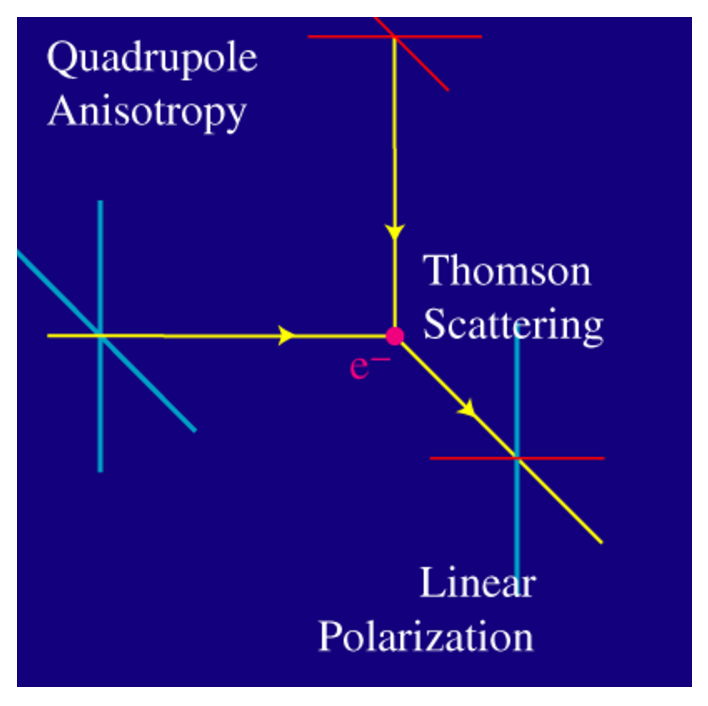
\includegraphics[width=8cm]{tauEPolarization.eps}
  \caption{An illustration (Wayne Hu, {\tt http://background.uchicago.edu/~whu/}) of how a net polarization signal is generated from Thompson scattering due to the presence of a quadrupole anisotropy. The blue cross and red cross show relatively strong and weak incident radiation, respectively, on an electron at the origin. The red/blue cross indicates the average polarization of scattered light and demonstrates that it obtains a net vertical polarization.			}
  \label{fig:tauEPolarization}
\end{figure}





\subsubsection{Kinetic Sunyaev-Zel'dovich Effect}

The second method of utilizing the CMB to constrain reionization that we discuss is the kinetic Sunyaev Zel'dovich effect (kSZ)\gloss{kSZ Effect}{Kinetic Sunyaev Zel'dovich effect. This describes secondary anisotropy in the CMB produced by the bulk velocities of free electrons during and after reionization which impart a Doppler shift on CMB photons.}. This refers to the secondary CMB anisotropies imprinted on the CMB by the bulk velocities of clouds of free electrons which impart a Doppler shift on the CMB photons. 


The kSZ signal is generally broken down into two contributions: the Doppler shift caused by bulk motions of free electrons \textit{after} reionization completes, and the Doppler shift due to the bulk motions of free electrons in ionized bubbles \textit{during} reionization. As such, the former contribution is known as the ``homogeneous'' (or, alternatively, Ostricker-Vishniac [OV]) kSZ signal and the latter is referred to the ``patchy'' kSZ signal. The homogeneous kSZ signal is sourced by density inhomogeneities on relatively linear scales and should be able to be modelled well (\citealt{mesinger2012kinetic}), allowing the isolation of the patchy contribution.


The patchy kSZ signal is actually sensitive to several parameters of reionization. First, unlike with $\tau_{e}$ measurements, the patchy kSZ contribution only arises \textit{during} reionization. Therefore, the magnitude of the signal itself is related to the duration of reionization since, for a longer reionization, CMB photons will have an opportunity to be Doppler shifted by ionized bubbles over a larger path length. Second, since the patchy kSZ signal is sourced by ionized bubbles, it will important at these bubbles' size scales and the strength of the signal will increase with patchier models of reionization. As such, a detection of a \textit{small} kSZ signal could also be indicative of a more homogeneous reionization, possibly with significant contributions from X-rays (\citealt{visbal2012gauging}).

The South Pole Telescope (SPT) attempted a measurement of this effect (\citealt{Zahn2012}) and interpreted the results in terms of a constraint on the duration of reionization, $\Delta z \equiv z_{\axhi=1} - z_{\axhi = 0.2}$. They were not able to make a detection of the effect but were able to place upper bounds on it, suggesting that $\Delta z < 7.9$ at 95\% confidence.\footnote{Technically, this constraint allows for a free parameter describing the level of correlation between the thermal SZ effect and the Cosmic Infrared Background. Without allowing for this free parameter, their constraint is $\Delta z < 4.4$ at 95\% confidence.}

\subsection{\lya\ Emitters}

\lya\ emitters (LAEs)\gloss{LAE}{\lya\ Emitter. These are galaxies which emit a significant fraction of their energy in the \lya\ line. This line is produced when hydrogen atoms within the galaxy recombine after being ionized by the galaxy. Roughly 2/3 of recombinations result in a \lya\ photon.} are galaxies which emit strongly in the \lya\ line. This \lya\ emission results from hydrogen atoms within the galaxy recombining after being ionized by the galaxy's UV radiation. During $\sim2/3$ of hydrogen recombinations, a \lya\ photon will be emitted. Therefore,  enough ionizations will result in a strong \lya\ line being emitted from the galaxy. 


However, whether or not that \lya\ line is observable to us depends on the intervening gas. Specifically, \lya\ photons produced within the galaxy will repeatedly be absorbed and re-emitted by hydrogen in the galaxy's interstellar medium until it reaches the IGM. At this point, if the IGM is ionized the \lya\ photon will escape. However, if the IGM is significantly neutral, then the \lya\ photon will be scattered into a low-surface-brightness halo, rendering the \lya\ line unobservable (\citealt{finlator2012recent}). This provides us with an observable which depends on the ionization state of the IGM! In this section, we briefly discuss two methods of utilizing this behavior in order to constrain $\axhi$.

%at \axhi = 0.5, LAEs residing in HII regions will typically be one of thousands that contribution to ionizing the HII regions. These regions can be \sim 10 Mpc. However, lya photons only need to travel 1 Mpc in order to redshift out of resonance and escape. 

\subsubsection{Clustering of \lya\ Emitters}

One approach for utilizing LAEs to constrain $\axhi$ is to look at their measured clustering. When the IGM is fully-ionized, the \lya\ lines of all observed galaxies should be visible to us. When the Universe is fully-neutral, then all observed galaxies should lack a strong \lya\ emission line. However, when reionization has progressed such that $\axhi \approx 0.5$, the Universe should represent a two-phase medium consisting of large ($\sim 10\mpch$) ionized regions maintained by thousands of galaxies (\citealt{McQuinn:2007dy}), and significantly-neutral regions which are shielded from the ionizing radiation. The \lya\ line from LAEs located within the large ionized regions should remain intact, as the photons will redshift out of \lya\ resonance after travelling only $\sim 1\mpch$ without encountering significantly-neutral hydrogen (\citealt{finlator2012recent}). Therefore, the LAEs observable when the Universe is 50\% ionized should more often reside in these ionized bubbles with many other sources, resulting in their observed distribution being \textit{highly clustered}. Meanwhile, at lower redshift, all LAEs should be observable (with regard to HI attenuation), resulting in a more uniform distribution.

In Figure \ref{fig:McQuinnLAEClustering}, \cite{McQuinn:2007dy} demonstrate this effect. The top row shows the ionization field (black is neutral, white is ionized) at three different neutral fractions: $\axhi = 0.7$ (left), 0.5 (middle), and 0.3 (right). The second row shows the true underlying LAE locations and the bottom row shows the observed LAEs. Since LAEs should only be observable within ionized regions, we see that the sources in the bottom row must coincide with white regions in the top row, resulting in enhanced clustering of the observed sources.

In \cite{Ouchi2010}, the authors analyze 207 LAEs at $z \sim 6-7$ and compare their clustering with those measured at $z = 5.7$. They find no detection of an enhancement in the observed LAE clustering, suggesting that the bulk of reionization occurred at $z > 6.6$. 



\begin{figure}[h]
  \centering
  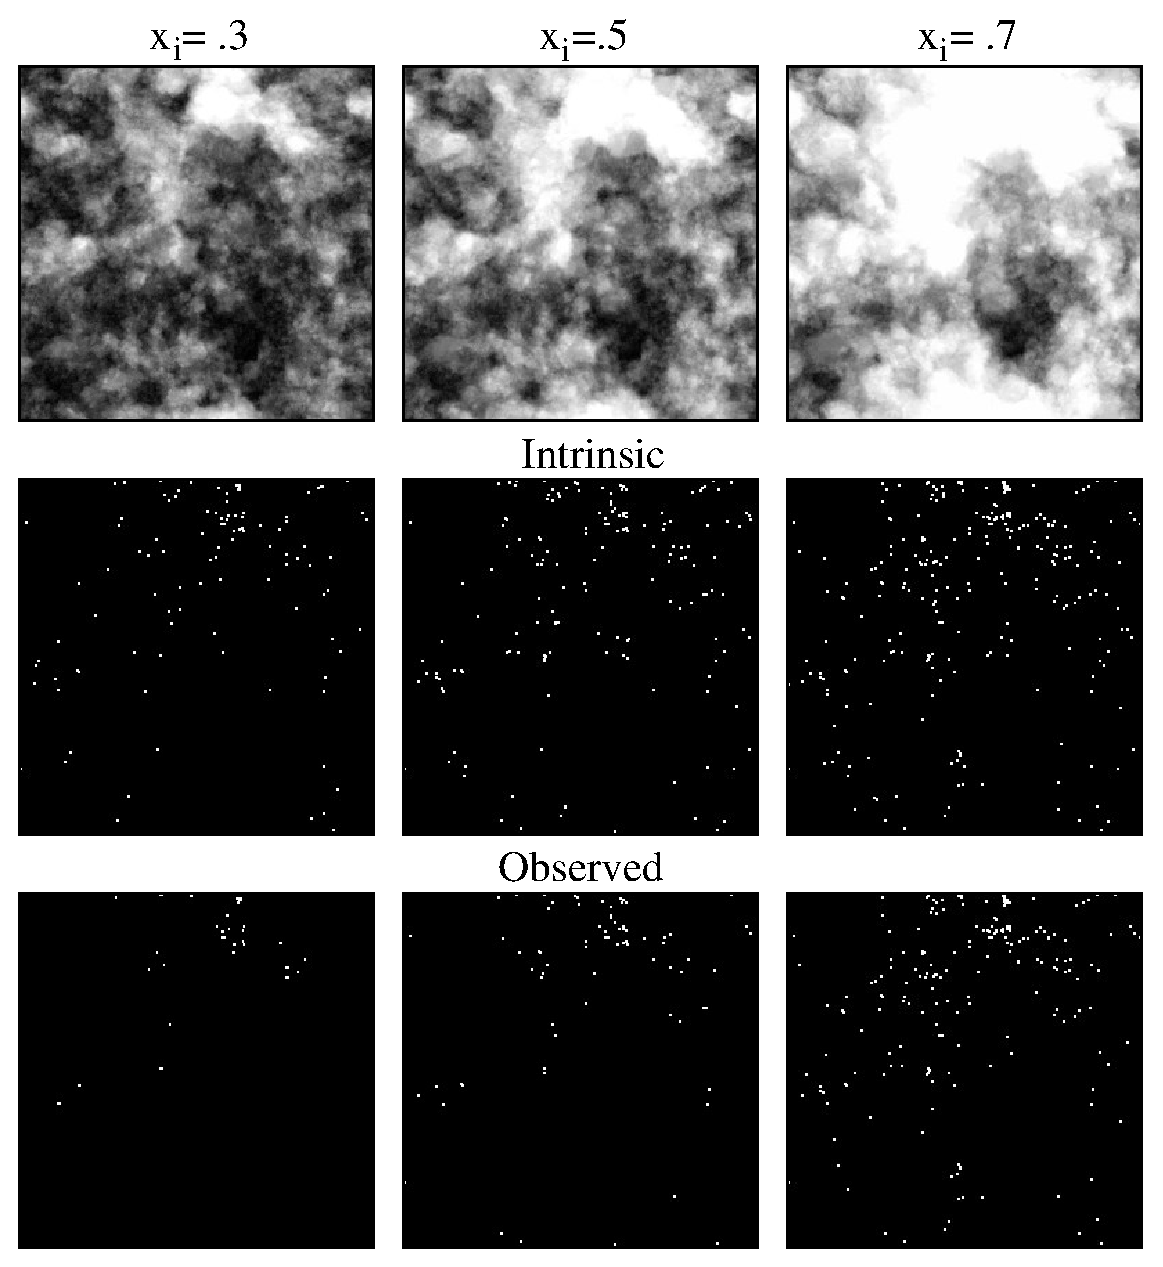
\includegraphics[width=13cm]{McQuinnLAEClusteringLarge.eps}
  \caption{The (simulated) effect of the neutral fraction on the observed clustering of LAEs (taken from \citealt{McQuinn:2007dy}). The top panels show the underlying ionization fields, the middle row shows the true location of LAEs in the simulation, and the bottom panel shows the detectable LAEs in the simulation. This shows that, LAEs which occupy the same ionized bubble will be observable, resulting in a less homogeneous field of observable LAEs. Each panel is 94 Mpc across. }
  \label{fig:McQuinnLAEClustering}
\end{figure}


\subsubsection{\lya\ Emitter Fraction}

As discussed in the previous section, as we move further back in redshift and deep into the reionization process, galaxies that intrinsically have a significant \lya\ line will not be observed as having one. However, the galaxies themselves will still be detectable via the drop-out technique, which searches for sources with significant emission at energies below the Lyman limit\gloss{Lyman Limit}{This refers to the most energetic transition in the Lyman series corresponding to ionizing a hydrogen atom in the ground state. This has wavelength $\lambda = 912$\AA and $E_{\gamma} = 13.6$eV.} and significantly less emission at greater energies. 


As we move further back in redshift, we expect the fraction of detected galaxies which \textit{would} have a \lya\ line but do not, due to a significantly-neutral IGM, will increase. While we do not have access to this exact measurement of this fraction, we \textit{can} measure the \textit{overall} fraction of detected galaxies which exhibit a strong \lya\ line, which should reflect the aforementioned trend. This has motivated the study of the evolution of the so-called ``\lya\ fraction'', denoted $f_{\text{\lya}}$ (\citealt{Schenker2012,pentericci2011spectroscopic,Pentericci:2014nia,caruana2012no,caruana2014spectroscopy}). This method has the benefit compared to some others, such as measuring the LAE luminosity function evolution, that some uncertainties due to the overall redshift evolution of observable galaxies, unrelated to the EoR, will drop out. 


Interestingly enough, some of these authors' analyses claim to support a surprisingly-neutral IGM. Specifically, work by \cite{caruana2014spectroscopy}, \cite{Pentericci:2014nia}, \cite{pentericci2011spectroscopic}, and \cite{Schenker2012} all suggest a neutral fraction of $\langle x_{\text{HI}}(z \sim 7) \rangle \sim 0.5$. This seems to be in tension with other constraints on the reionization process. Namely, in \S \ref{sec:CMB}, we discussed constraints on the redshift of ``instantaneous reionization'', which can be interpreted as an upper bound on the mid-point of reionization, of $z_{r} = 8.8^{+1.3}_{-1.2}$ (\cite{planck2015planck}). Additionally, analysis by \cite{Bolton:2007b} suggests that reionization is a rather extended process. Assuming this $f_{\text{Ly}\alpha}$ constraint is correct, this would allow only $\Delta z \sim 1$ for the second half of reionization to complete. 


One plausible way to reconcile these observations is presented by \cite{2013MNRAS.429.1695B} who suggest that the rise in the prevalence of dense absorbers at high $z$, rather than a rise in the neutral fraction of the diffuse IGM, could contribute to a surprisingly-small $f_{\text{Ly}\alpha}$ without requiring changes in the neutral fraction of tens of per cent over $z \sim 6-7$. Furthermore, \cite{Taylor:2013qia} argue that, due to the expected large-scale inhomogeneity of reionization, LAE surveys which sample relatively small regions of the sky are subject to sample variance which can mitigate the high-neutral-fraction requirements. However, their analysis still suggests that $\axhi > 0.05$ at 95\% confidence. Thus, while the precise amount of neutral hydrogen required to explain the $f_{\text{Ly}\alpha}$ observations is controversial, it is exciting that the conclusion we are observing some phase of reionization is rather robust. 

% papers to cite
% detect something
% \cite{Schenker2012}
% \cite{pentericci2011spectroscopic}
% \cite{Pentericci:2014nia}
% \cite{Pentericci:2014nia}
% \cite{caruana2012no}
% \cite{caruana2014spectroscopy}
% don't
% 


\subsection{Luminosity Function Measurements}

One last method that we will discuss for constraining the Epoch of Reionization is through luminosity function\gloss{Luminosity Function}{A function that describes the number, or number density, of sources with a given luminosity.} measurements. Luminosity functions describe the number of sources, in this case galaxies, as a function of luminosity. With knowledge of the luminosity function, the ionizing luminosity of galaxies within a given luminosity bin, and of the escape fraction of ionizing photons over a range of redshifts, it should be possible to determine if enough ionizing photons were produced by a given redshift in order to ionize the Universe and keep it that way. 





\section{Where We Stand}

%\begin{enumerate}
%\item Bouwens et al. (2015) might be good to include here. Strengthens argument that galaxies reionized the Universe and that quasars/AGN did not.
%\end{enumerate}
% ----------------------------------------------------------------------



	


% the code below specifies where the figures are stored
\ifpdf
    \graphicspath{{neutral_islands/figures/PNG/}{example_chapter/figures/PDF/}{neutral_islands/figures/}}
\else
    \graphicspath{{neutral_islands/figures/EPS/}{neutral_islands/figures/}}
\fi


% ----------------------------------------------------------------------
%: ----------------------- content ----------------------- 
% ----------------------------------------------------------------------
\chapter{How to Search for Islands of Neutral Hydrogen in the $z \sim 5.5$ IGM}
\section{Introduction} \label{sec:intro}


It has been nearly half a century since \citet{1965ApJ...142.1633G} pointed out that the lack of prominent
absorption troughs, blueward of the Ly-$\alpha$ line in quasar spectra, implies that intergalactic
hydrogen is highly ionized. 
Only in the year 2001 were 
complete ``Gunn-Peterson'' absorption troughs finally revealed in 
the Ly-$\alpha$ forest of high redshift ($z \gtrsim 6$) quasars discovered using the Sloan Digital Sky Survey (SDSS)
\citep{Fan:2001ff,Becker:2001ee,Djorgovski:2001ez}. 
Although these prominent absorption troughs were discovered more than a decade ago, the precise interpretation
of the observations, and their implications for the reionization history of the universe,
remain unclear. One difficulty here relates to the large optical depth to
Ly-$\alpha$ absorption: near $z \sim 6$, the optical depth 
is $\tau_\alpha \sim 4 \times 10^5$ in a fully neutral IGM at the cosmic mean density \citep{1965ApJ...142.1633G}. Based on this, it is common to infer 
that the IGM must be highly ionized below $z \lesssim 6$,
at which point quasar spectra do show some transmission through the Ly-$\alpha$ line. In addition, it is clearly hard
to discern whether the gas above $z \gtrsim 6$ -- that does show complete absorption in the Ly-$\alpha$ line --
is mostly neutral or is only neutral at the level of about one part in ten-thousand or so (e.g. \citealt{Fan:2005es}); in either case,
the Ly-$\alpha$ line will be completely absorbed.

However, if reionization is sufficiently inhomogeneous and ends late, there may be some transmission through
the Ly-$\alpha$ forest {\em before reionization completes} \citep{Mesinger:2009mv,Lidz:2007mz}. Theoretical models of reionization show that
the IGM during reionization resembles a two-phase medium, containing a mixture of highly ionized
bubbles along with mostly neutral regions. The ionized bubbles grow and merge, eventually filling essentially the entire
volume of the IGM with ionized gas; the redshift at which this process completes is highly uncertain and still awaits definitive empirical constraint. In principle, the ionized bubbles may allow transmission through the
Ly-$\alpha$ forest even when some of the IGM volume is still in fact filled by neutral regions, i.e., before reionization completes.
This calls into question the conventional wisdom described above -- that the presence of transmission through the $z \lesssim 6$ forest
necessarily implies reionization completed by $z=6$ \citep{Lidz:2007mz,Mesinger:2009mv} -- strictly speaking, this conclusion follows only in 
the unrealistic case of a homogeneously-ionized
IGM. 

Indeed, some portions of the $z \sim 5-6$ Ly-$\alpha$ forest are completely absorbed, while other portions of the forest at these redshifts show
transmission through the Ly-$\alpha$ line. 
Quantitatively, if one counts only the fraction of pixels with some transmission
through the forest as ``certain to be ionized'', the volume-averaged neutral hydrogen fraction need only be smaller than 
$\avg{x_{\rm HI}} < 0.2$ at $5 \leq z \leq 5.5$, and smaller than $\avg{x_{\rm HI}} < 0.5$ at $z=6$ \citep{McGreer:2011dm}.
These constraints are conservative since even mostly-ionized gas will give rise to some completely absorbed regions at these redshifts, 
but it is nevertheless interesting to ask whether some of the absorbed regions could in fact
come from remaining ``islands'' of mostly neutral hydrogen gas in the IGM. The dark pixel fraction constraints of \citet{McGreer:2011dm} certainly leave
plenty of parameter space open for reionization completing at $z \leq 6$. 

In fact, there are hints -- albeit indirect ones -- that significant
amounts of neutral gas may remain in the IGM at these late times and so 
we believe that investigating this possibility amounts to {\em more} than closing a remaining ``loophole'' in the analysis
of the $z \lesssim 6$ Ly-$\alpha$ forest. For example, recent measurements of the rest-frame ultraviolet galaxy luminosity function 
suggest a relatively low ionizing emissivity at $z \gtrsim 5-6$, even for seemingly generous assumptions
about the escape fraction of ionizing photons ($f_{\rm esc} \sim 0.2$) and allowing significant extrapolations down the faint end of the luminosity function;  e.g. the preferred model
of \citet{Robertson:2013bq} (that matches these observations) has $\axhi = 0.1$ at $z=6$. In addition, the fraction of Lyman-break galaxies with detectable Ly-$\alpha$ emission lines shows evidence
for a rapid drop between $z \sim 6-7$ which may require a significant neutral fraction at $z \sim 7$ (e.g., \citealt{2012ApJ...744..179S,Pentericci:2014nia}, although see \citealt{2013MNRAS.429.1695B,Taylor:2013qia}). The inferred $z \sim 7$ neutral fraction here would be easier to accommodate if there is
still some neutral gas at $z \leq 6$.  Furthermore, \citet{Becker:2014oga} recently discovered an impressive $\sim 110$ Mpc/$h$ dark region in the $z \sim 5.7$ Ly-$\alpha$ forest. This may result from an upward opacity fluctuation -- driven by a fluctuating ultraviolet radiation field in a mostly ionized IGM -- but this striking observation invites contemplating the more radical possibility that diffuse neutral regions remain in the IGM at this late time.
Finally, \citet{Mesinger:2006kn} and \citet{2013MNRAS.428.3058S} argue that the proximity zones of quasars at $z \geq 6$ show evidence for damping wing absorption and a significant neutral fraction, further motivating the search for neutral gas at slightly later times.


Perhaps more importantly, we can design robust observational tests for the presence of neutral islands in the $z \sim 5.5$ IGM, and either
definitively detect neutral hydrogen at these redshifts, or significantly improve on the existing upper limits from \citet{McGreer:2011dm}. 
Towards this end, we study three possible tests for identifying neutral islands in the $z \sim 5-6$ IGM, each of which 
can be applied using existing 
Ly-$\alpha$ forest spectra. The presence of some transmission through the Ly-$\alpha$ forest at $z \leq 6$ allows us to consider
tests that can not be applied at still higher redshift where the forest is 
completely absorbed (asides for in the ``proximity zones'' close to the quasar itself). 
We develop these tests using mock quasar spectra extracted from the numerical reionization simulations of
\citet{McQuinn:2007dy}.
The first test we consider has been studied before (e.g. \citealt{Fan:2005es}, \citealt{2010MNRAS.407.1328M}, \citealt{McGreer:2011dm}), but is the most model 
dependent: the abundance and size distribution of ``dark gaps'', i.e., regions of saturated absorption in the Ly-$\alpha$ forest. Here we focus on
the plausible impact of inhomogeneous reionization on the dark gap statistics. The second test utilizes the fact that the natural line width of the Ly-$\alpha$ line gives rise to extended damping wing absorption, in
the case that highly neutral gas is present in the IGM \citep{MiraldaEscude:1997qb}. As a result, the transmission recovers more
slowly around significantly neutral absorbed regions than around absorbed yet ionized regions. We find that this
signature can be detected in partly neutral models by examining the stacked profile around extended absorbed regions. Note that, in contrast to previous work, here we propose to search
for the damping wing signature in typical regions of the IGM, as opposed to in the proximity zones of quasars (\citealt{Mesinger:2006kn,2013MNRAS.428.3058S}), or redward of Ly-$\alpha$ at the source redshift. 
Our third test involves the stacked profile
of extended absorbed regions in the Ly-$\beta$ forest. If these regions are significantly neutral, there should be a feature
from absorption in the deuterium Ly-$\beta$ line just blueward (but not redward) of absorbed regions.

The outline of this paper is as follows. In \S\ref{sec:Viability}, we briefly discuss which range of (volume-averaged) neutral fractions are physically plausible at $z=5.5$. In 
\S \ref{sec:Sims} we describe the simulations used and the process for generating mock spectra. We discuss how the dark gap size distribution may be used to constrain the neutral fraction in \S \ref{sec:HIDistributions}. In \S \ref{sec:Stacking}, we describe how quasar spectra may be stacked in order to reveal the presence of deuterium and HI damping wing absorption in an idealized scenario and discuss adapting this approach for more realistic spectra in \S \ref{sec:RealSpectra}. We then apply this approach to mock quasar spectra in \S \ref{sec:Results}, discuss the constraining power of the stacking approaches in \S \ref{sec:Forecasts}, and conclude in \S \ref{sec:Conclusion}. Throughout, we consider a $\Lambda$CDM cosmology parametrized by $n_{s} = 1$, $\sigma_{8} = 0.8$, $\Omega_{m} = 0.27$, $\Omega_{\Lambda} = 0.73$, $\Omega_{b} = 0.046$, and $h = 0.7$, (all symbols have their usual meanings), broadly consistent with recent Planck constraints from \cite{Ade:2013zuv}.


\section{Viability of Transmission Through a Partially Neutral IGM} \label{sec:Viability}

 
 Ideally, this study would make use of mock Ly-$\alpha$ forest spectra extracted from fully self-consistent simulations of reionization, in which the efficiency of the ionizing sources and other relevant parameters are tuned so that reionization completes at $z \leq 6$.
 Unfortunately, large-scale reionization simulations that simultaneously resolve the properties of the gas distribution, as well as the sources and sinks of ionizing photons, while
 capturing large enough volumes to include a representative sample of the ionized regions, are still quite challenging. Here, we instead explore more approximate, yet more flexible, models.
 As we describe in more detail in the next section, we make use of the reionization simulations of \citet{McQuinn:2007dy} to describe the size  and spatial distribution of the ionized and
 neutral regions during reionization. Inside of the ionized regions, we rescale the simulated photoionization rates, adjusting the intensity of the UV radiation field to match the observed mean transmitted flux through the Ly-$\alpha$ forest.
 For simplicity, we assume  that the intensity of the UV radiation field in the ionized regions is uniform and comment on the possible impact of this approximation where relevant.
 
 Before proceeding further, however, it is worth considering which (volume-averaged) neutral fractions are physically plausible near $z \sim 5.5$. In order to get transmission through
 the $z \sim 5.5$ Ly-$\alpha$ forest, at least some of the hydrogen needs to be highly ionized.  This requires the mean free path of ionizing photons to be relatively large, although we should keep in mind that the attenuation length will vary spatially during and after reionization, and so this quantity needs to be large only across some stretches of the IGM.
 This in turn demands some minimum separation between the neutral islands, because otherwise the neutral islands themselves will limit the mean free path and prevent a sufficiently
 intense UV radiation field from building up between the islands. Hence, it may be inconsistent to have remaining neutral islands in the IGM, yet still have some transmission through the Ly-$\alpha$ forest. Here we briefly quantify this reasoning; we will be content with only a rough estimate, as our focus
here is more on designing empirical tests. Further theoretical
exploration here might be valuable, however, perhaps along the lines of \cite{Xu:2013npa}. 

Quantitatively, previous studies infer that a photoionization rate on the order of $\Gamma_{\rm HI} \sim 5 \times 10^{-13} \text{s}^{-1}$ is required to match the mean transmitted flux in the
$z \sim 5.5$ Ly-$\alpha$ forest (e.g., \citealt{KuhlenConcordance}, \citealt{Bolton:2007b}).\footnote{Theses studies assume that reionization is complete at these redshifts. If the universe is in fact partly neutral, then a higher photoionization rate should be required in the ionized regions. In our rough estimate here, we neglect this given the other significant uncertainties involved.}
If we demand that the photoionization rate between the neutral islands needs to be in this ballpark to allow transmission through the forest, we can translate this into a required minimum average separation
between the neutral islands, given an assumed ionizing emissivity. The average ionizing emissivity is likely on the order of $\epsilon_{\rm HI} \sim 3$ photons per atom per Gyr (e.g. \citealt{Bolton:2007b}).
This is close to the value required simply to balance recombinations and maintain the ionization of the IGM at the redshifts of interest. This emissivity is also comfortable with that inferred from the above
photoionization rate and measurements of the mean free path to ionizing photons (\citealt{Bolton:2007b}, although \citealt{Becker:2013ffa} recently argued for a slightly larger value), as well as the UV emissivity implied by measurements of the galaxy luminosity function (e.g. \citealt{Robertson:2013bq}).
  

In this context, it is useful to note that:
\begin{align}
\Gamma_{\text{HI}} &= \varepsilon_{\text{HI}} \sigma_{\text{HI,lim}} \lambda_{\text{mfp}} \dfrac{\beta}{\beta + 1.5},
\end{align}
where $\varepsilon_{\text{HI}}$ is the average proper ionizing emissivity, $\sigma_{\text{HI,lim}} = \pow{6.3}{-18}\text{cm}^{2}$ is the photoionization cross section at the Lyman limit, $\lambda_{\text{mfp}}$ is the mean free path of ionizing photons at the Lyman limit, and $\beta$ is the intrinsic, unhardened spectral index of the ionizing radiation.  This expression assumes that the mean free path to ionizing photons
propagating through a clumpy IGM scales as $\nu^{3/2}$ \citep{Zuo}.
Inserting typical numbers we find:
\begin{align}
\Gamma_{\text{HI}} &= \pow{5.0}{-13} \text{sec}^{-1} \left[ \dfrac{\varepsilon_{\text{HI}}}{3\ \text{photons}/\text{atom}/\text{Gyr}}  \right]\\
& \times \left[ \dfrac{\beta}{2} \right] \left[ \dfrac{3.5}{1.5 + \beta} \right] \left[ \dfrac{1 + z}{6.5} \right]^{3} \left[ \dfrac{\lambda_{\text{mfp}}}{9.1 \ \text{pMpc}} \right].
\end{align}
In other words, to get transmission through the forest for plausible values of the ionizing emissivity, we require the mean separation between neutral islands to be
$\lambda_{\rm min} \gtrsim \lambda_{\text{mfp}} \gtrsim 9.1 {\text{pMpc}}$. This is a minimal requirement in that it assumes  the neutral islands set the mean free path, when in fact
Lyman limit systems and cumulative absorption in the mostly ionized gas may also play a role. On the other hand, the required minimum separation between the neutral islands would 
go down if a smaller $\Gamma_{\text{HI}}$ suffices to allow transmission through the forest, or if the ionizing emissivity is in fact higher. 
However, the mean free path to ionizing photons has
recently been measured at $z = 5.16$ to be $\lambda_{\text{mfp}} = 10.3 \pm 1.6 \text{pMpc}$ \citep{Worseck:2014fya}, only somewhat larger than our assumed $\lambda_{\text{mfp}}$ here. While there are still uncertainties, and while the measured mean free path scales steeply with redshift ($\lambda_{\text{mfp}} \propto (1+z)^{5.5}$), viable models are unlikely to have neutral islands spaced much more closely than this. 



We can then use this requirement on $\lambda_{\text{mfp}}$ to get some sense of which volume-averaged neutral fractions are plausible at $z \sim 5.5$. In the simulation outputs considered here (see \S\ref{sec:Sims}), the 
mean separation between neutral islands is $\lambda_{\text{mfp}} = 17.0$ pMpc, 5.3 pMpc, and 2.7 pMpc for $\axhi = 0.05$, 0.22, and 0.35, respectively. The first case certainly satisfies
the requirement described above, the second case is just a bit on the small side, while the third case is uncomfortably small. Given the uncertainties in this argument, and the possibility that the neutral
islands are a bit larger than in our simulation (which would increase their mean separation at fixed filling factor), we consider all three cases, but refrain from considering still more neutral models. We regard the latter case ($\axhi = 0.35$) as an extreme scenario intended mostly for illustration. 

 
Finally, it is worth keeping in mind that any remaining neutral islands will likely be photoionized on a short timescale. For example, using Eq. 1 in \citet{Lidz:2014jxa} with $C=3$, $M_{\rm min} = 10^9 M_\odot$, and
$\zeta = 20$, the redshift interval over which the volume average ionized fraction transitions from $\avg{x_i} = 0.8$ to $\avg{x_i}=1$ is only $\Delta z \sim 0.5$. 
However, it is possible that we
are catching this -- likely brief -- phase in $z \sim 5.5$ Ly-$\alpha$ forest
spectra and the possibility of testing this remains tantalizing.


\section{Simulations and Mock Spectra} \label{sec:Sims}


With the above discussion to frame the range of possibilities, we move to describe the numerical simulations used in this analysis and our approach to constructing mock Ly-$\alpha$ forest
absorption spectra before reionization completes. We use simulated density and ionization fields generated from a dark matter simulation of \cite{McQuinn:2007dy} which tracks $1024^{3}$ dark matter particles in a simulation volume with a co-moving sidelength of $L = 130\mpch$. We assume that the gas closely follows the dark matter. In this work, we focus on redshift $z = 5.5$, but consider several possible neutral fractions. In practice, we obtain ionization fields with higher (lower) neutral fractions by using simulation outputs at higher (lower) redshifts. This should be an appropriate approximation since the statistical properties of ionized regions at a given neutral fraction are most sensitive to the neutral fraction and are relatively insensitive to the redshift at which the neutral fraction was attained (see \citealt{McQuinn:2006et} and \citealt{Furlanetto:2004nh}).
 
 
We generate mock quasar spectra according to the usual ``fluctuating Gunn-Peterson" approach (e.g., \citealt{Croft:2000hs}), with a few refinements to capture the main effects of incomplete reionization. First and foremost, we do not assume a fully ionized IGM. The transmission in the Ly-$\alpha$ forest is sensitive to the precise ionized fractions in the ionized phase of the IGM. In order to simplify our study, as mentioned in the previous section, we rescale the simulated photoionization rates in the ionized regions to match the observed mean transmitted flux through the Ly-$\alpha$ forest. We do this assuming
ionization equilibrium, and a constant value of the UV background (with a photoionization rate per atom of $\Gamma_{\text{HI}}$) within ionized regions. Specifically, simulated pixels with $x_i > 0.9$ are considered highly ionized while less ionized pixels are considered fully neutral.\footnote{After effectively thresholding the ionization field in this way, we end up with neutral fractions which are $\approx 20\%$ higher than in the original simulation. Throughout the paper, we refer to increased, thresholded neutral fractions.} This simplified approach allows us to consider a range of different possibilities for
the ionization state of the IGM quickly. We comment on the shortcomings of this approach when appropriate.
The optical depth of a given pixel, $i$, in the simulation can then be found by summing over contributions from neighboring pixels (Bolton \& Haehnelt 2008):
\begin{align}
\tau_{\alpha}(i) &= \frac{c \sigma_{\alpha}\delta R}{\pi^{1/2}}\sum_j \frac{n_{\text{HI}}(j)}{b(j)}H(a,x),
\end{align}
where $b(j) = (2 k_{\text{B}}T(j)/m_{p})^{1/2}$ is the Doppler parameter, $T(j)$ is the temperature of pixel $j$, $\delta R$ is the pixel proper width, $\sigma_\alpha = \pow{4.48}{-18}\text{cm}^{2}$ is the \lya\ scattering cross section, $m_p$ is the proton mass, $H(a,x)$ is the Hjerting function, and $n_{\text{HI}}(i)$ is the number density of hydrogen atoms at pixel $i$, found using the simulated density field. To calculate the Doppler parameter, we assume that the gas obeys a modified temperature-density relationship
\begin{align}
T(\delta) = \begin{cases} T_0(1 + \delta)^{\gamma - 1} &\mbox{if ionized}\\
1,000 \text{K} &\mbox{if neutral}, \end{cases} \label{eq:TDrelation}
\end{align}
where $\delta$ is the matter overdensity in units of the cosmic mean and we choose $T_{0} = \pow{2}{4}$K and $\gamma = 1.3$ as the temperature at mean density and slope of the temperature-density relation, respectively. For simplicity, we assume the ionized gas lies on the aforementioned temperature-density relation, although there should be significant scatter around this relation close to
reionization (e.g. \citealt{Lidz:2014jxa}). We do not expect this to impact our conclusions significantly. The neutral gas should be colder than the ionized gas, of course, with a temperature set perhaps by low levels of X-ray pre-heating. Here
we adopt $T =1,000$ K for the neutral gas; this choice is likely a bit large (it was chosen partly for ease in computing the Hjerting function below), but we have checked that we get nearly identical results for colder temperature choices.


The Hjerting function is a convolution of a Lorentzian profile, which incorporates the natural line profile of the Lyman-series lines, with a Maxwell-Boltzmann distribution, which accounts for the effects of thermal broadening on the line profile. The Hjerting function is defined by:
\begin{align*}
H(a,x) &= \frac{a}{\pi} \int_{-\infty}^{\infty}\frac{e^{-y^2}\dd y}{a^{2}+ (x-y)^2},
\end{align*}
where $a = \Lambda_{\alpha} \lambda_{\alpha}/4\pi b(j)$, $\Lambda_{\alpha} = \pow{6.265}{8}\sec^{-1}$ is the damping constant, $\lambda_{\alpha} = 1215.67 \text{\AA}$ is the \lya\ wavelength, $x$ is the relative velocity of pixel $i$ and pixel $j$ in units of the Doppler parameter, defined as $x = \left[ v_{\text{H}}(i) - u(j) \right]/b(j)$, where $u(j) = v_{\text{H}}(j) + v_{\text{pec}}(j)$. The peculiar velocity field is generated by applying linear perturbation theory to the underlying density field.\footnote{This was done because the full peculiar velocity field was not readily available, but this approximation should not impact our results.}  In detail, the natural line profile is only approximately described by a Lorentzian \citep{Lee:2013fga}, with asymmetric corrections becoming important far from line center. In this study, the
precise shape of the damping wing far from line center is unimportant: we make use only of the gradual recovery in transmission around saturated neutral regions, rather than the detailed shape of this
recovery, which is also strongly influenced by neighboring neutral regions. We hence expect the Lorentzian form to be a good approximation for our present purposes.


In addition to including absorption from the hydrogen damping wing, we also include absorption from primordial deuterium. As a result of big bang nucleosynthesis, primordial hydrogen should be accompanied by traces of deuterium, with a relative abundance by number of $\text{D}/\text{H} = 2.5\times 10^{-5}$ (\citealt{Cooke:2013cba}). Due to its slightly increased reduced mass, Lyman series transitions in deuterium will be shifted blueward by 82\kms\ compared to the same transitions in hydrogen. We account for deuterium by scaling the number density of hydrogen in a given pixel by the relative abundance and shifting the resulting optical depths blueward by 82\kms. Additionally, the Doppler parameter is adjusted to $b_{\text{D}}(j) = \left( 2k_{\text{B}}T(j)/(2m_{p}) \right)^{1/2}$ to account for the increase in mass.

In this work, we focus mostly on $z=5.5$ and adopt a mean transmitted flux at this redshift of $\avg{F}=0.1$, consistent with determinations from e.g., \cite{Becker:2001ee}. In some cases, we test the
sensitivity of our results to the mean transmitted flux by considering $\avg{F}=0.05$ as well. In general, the lower the mean transmitted flux, the more challenging it is for us to identify any remaining
neutral islands. On the other hand, the likelihood that neutral islands remain increases towards high redshift and decreasing mean transmitted flux. As mentioned previously, we rescale the simulated photoionization rates in the ionized regions to a uniform value,
normalized so that an ensemble of mock spectra matches the observed mean transmitted flux. It is important to note that the mean transmitted flux is a very steep function of redshift near $z \sim 5.5$, and that the sightline-to-sightline scatter in this quantity is substantial \citep{Fan:2005es}, and so one may want to carefully test for sensitivity to the precise redshift binning used.


We use the same approach as described above to generate \lyb\ mock spectra, with $\lambda_{\beta} = 1025.72\text{\AA}$, $\Lambda_\beta = \pow{1.897}{8}\sec^{-1}$, and $\sigma_\beta = \pow{7.18}{-19}\cm^{2}$. However, in generating \lyb\ mock spectra, we must also account for foreground \lya\ absorption due to gas at lower redshifts, $\lambda_\alpha (1+z_{\text{Ly}\alpha}) = \lambda_{\beta}(1 + z_{\text{Ly}\beta})$, where $z_{\text{Ly}\alpha}$ is the redshift of the foreground \lya\ absorber and $z_{\text{Ly}\beta}$ is the redshift of the \lyb\ absorber. We will assume we are investigating quasar spectra at $z_{\text{Ly}\beta} =  5.5$ for this work, such that the corresponding foreground \lya\ absorption in the \lyb\ spectra occurs at redshift $z_{\text{Ly}\alpha} = 4.5$. We adjust $\Gamma_{\text{HI}}$ for the foreground \lya\ absorption to match measurements of the mean transmission from \cite{2013MNRAS.430.2067B} at these redshifts ($\left\langle F \right\rangle \approx 0.31$ at $z = 4.5$).\footnote{We generate foreground \lya\ absorption by considering the absorption from regions in the same simulation box, but demand that they are widely-separated from the high redshift regions of interest ($>10\mpch$). This enforces that the underlying density fields sourcing the \lyb\ absorption and the foreground \lya\ absorption are uncorrelated, as should be the case for actual spectra.} The optical depth of a pixel in a \lyb\ spectrum is then the sum of the contribution from the foreground \lya\ absorption and the intrinsic \lyb\ absorption $\tau_\beta^{\text{tot}}(z_{\text{Ly}\beta}) = \tau_{\beta}(z_{\text{Ly}\beta}) + \tau_{\alpha}(z_{\text{Ly}\alpha})$.


In \Fig{fig:ExampleSpectraA}, we show an example mock \lya\ spectrum for a particular line of sight through the simulation. We show only a portion of the line of sight in order to exhibit smaller-scale features. The top figure shows the \lya\ transmission when the hydrogen damping wing is neglected (black) and when it is included (dashed red), while the bottom panel shows the underlying thresholded ionization field. We have neglected peculiar velocities in creating this figure in order to facilitate a comparison between the spectrum and the underlying ionization field. 


From this figure, we see that the damping wing indeed has a significant effect on the transmission, but that its effect is hard to discern without knowing the damping-wing-less transmission. This is the case for two reasons. First, the forest here is very absorbed and the damping wing absorption becomes mixed with resonant absorption from neighboring ionized regions. Second, the damping wing from a particular neutral region may overlap with the damping wing from another neutral region, altering the shape of the resulting absorption. Specifically, we see that, in the example spectra, the region at $v \approx 4500\ \kms\ $ is sandwiched between HI regions to the left and right, both within 1000\kms. Therefore, the optical depths for the corresponding pixels likely have significant contributions from resonant absorption, damping wing absorption from the HI region to the left, and damping wing absorption from the HI region to the right. While detecting individual instances of damping wing absorption in this case 
seems impossible, we will show that detecting the presence of damping wing absorption \textit{on average} should be feasible through the stacking of high-redshift quasar spectra.

\begin{figure}[h]
  \centering
  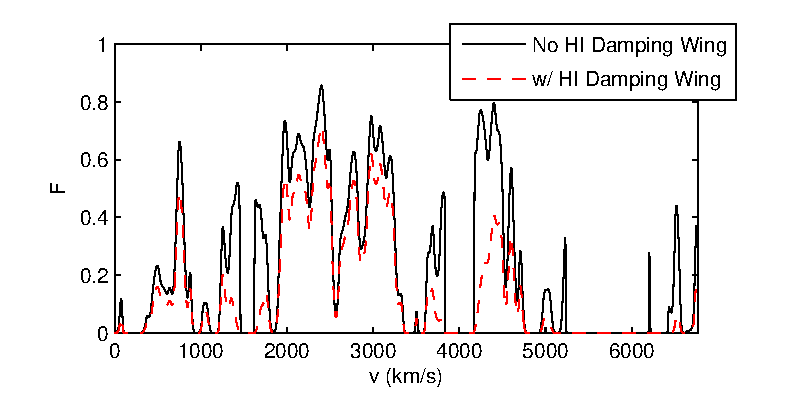
\includegraphics[width=9cm]{fig1a.eps}
  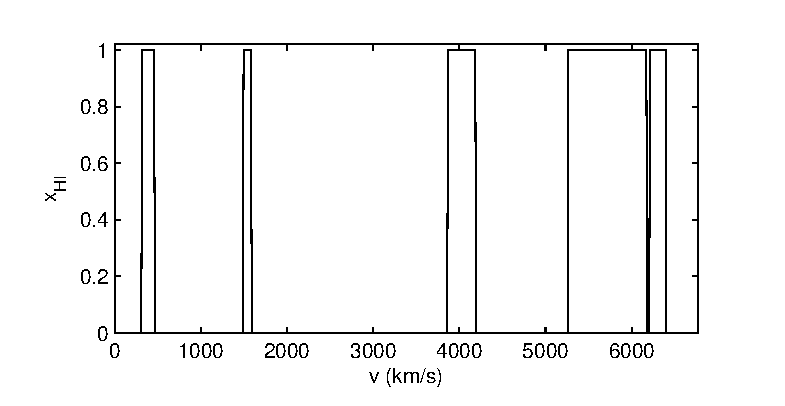
\includegraphics[width=9cm]{fig1b.eps}
  \caption{Example mock \lya\ forest spectrum and corresponding neutral fraction. The top panel shows the \lya\ transmission while the bottom panel is the neutral fraction along the line of sight, with ionized regions set to $x_{\rm HI} \approx 0$ for illustration. The black curve in the top panel shows the transmission through the forest when absorption due to the hydrogen damping wing is neglected, while the red curve includes damping wing  absorption. The comparison illustrates that damping wing absorption has a prominent impact, but it is also clear that the presence of the damping wing will be hard to discern by eye. The line of sight is extracted from a model with $\axhi = 0.22$, but note that we have deliberately chosen a sightline with more neutral regions than typical.}
  \label{fig:ExampleSpectraA}
\end{figure}




\section{Dark Gap Statistics} \label{sec:HIDistributions}


With the mock spectra of the previous section in hand, we now consider the size distribution of regions of saturated absorption -- dark gaps -- and its dependence on the underlying neutral fraction. Using such dark gap statistics has been widely discussed as a potential probe of the IGM neutral fraction (see, e.g., \citealt{Fan:2005es}, \citealt{Gallerani:2005mf}, \citealt{2010MNRAS.407.1328M}, \citealt{McGreer:2011dm}). In a fully ionized IGM, the size of dark gaps in quasar spectra should grow with increasing redshift, simply owing to the increasing mean density of the universe and as a result of any decline in the intensity of the UV radiation background. However, once quasar spectra start to probe the tail end of reionization, the increase in dark gap size should accelerate due to the presence of islands of neutral hydrogen. 

In \Fig{fig:DarkGapHist}, we have plotted the size distribution of dark gaps, $\text{d}P(L)/\text{d}\ln L$, in blue for the $\axhi = 0.22$ mock spectra, assuming a mean transmission of $\langle F \rangle = 0.1$. Additionally, the dashed curves display the two underlying populations of dark gaps: those sourced by ionized gas (magenta) and those sourced by neutral gas (cyan). For clarity, we only show dark gaps larger than $L_{\text{sat,min}} = 0.7\mpch$ ($\sim 90 \kms$), since smaller saturated regions will be predominantly ionized. Additionally, we have neglected peculiar velocities when generating spectra here. Two important points become apparent from this figure. First, at $ L \sim 8.5\mpch$ ($\sim 1100 \kms$), dark gaps transition from being primarily sourced by ionized gas to being primarily sourced by neutral gas. This reinforces our intuition that, in a partially neutral IGM, the largest dark gaps should correspond to the remaining neutral islands. Second, the dark gaps being composed of two different populations gives rise to a bimodality in the size distribution. This suggests that the behavior of the large-$L$ tail of the size distribution may offer additional information about the neutral fraction, with a steep decline suggesting a highly ionized IGM and a more gradual decline, or the emergence of a second peak, suggesting a significantly neutral IGM. Such a ``knee" in the dark gap size distribution is also mentioned in \cite{2010MNRAS.407.1328M}.


Additionally, we can consider the large-$L$ tail of the size distribution and its dependence on neutral fraction at a fixed mean transmission. In \Fig{fig:PDFs}, we plot an expected histogram of dark gap sizes for 10 spectra for  $\axhi = 0$ (magenta), 0.05 (cyan), 0.22 (blue), and 0.35 (black), again assuming that $\langle F \rangle = 0.1$. Three trends become obvious from this plot. First, as the neutral fraction is increased (at fixed $\langle F \rangle $), the number of large saturated regions increases and, second, as the neutral fraction is increased, the size of the largest dark gaps also increases. For example, in the $\axhi = 0.22$ model, the largest dark gaps are roughly five times bigger than in the fully ionized model. Additionally, we again see hints of the underlying dark gap size distribution being bimodal as the neutral fraction is increased, supporting the idea that the \textit{shape} of the dark gap size distribution may be a diagnostic for the underlying neutral fraction.


Given these trends, it should be possible to compare dark gap distributions from observed spectra against models at various neutral fractions and use this to constrain the mean neutral fraction of the IGM. This approach is appealing in that it does not require especially high-resolution or high signal-to-noise spectra. However, it does require comparison with simulated models 
of the dark gap
size distribution and so the conclusions reached will be somewhat model dependent.
Additionally, the distributions are dependent on the assumed mean transmission, which is itself uncertain. In particular, estimates of the mean transmission at high redshift may be impacted by continuum
fitting errors, given the inherent difficulty in estimating the unabsorbed continuum level in highly-absorbed spectra.


In order to investigate the impact of possible continuum fitting errors, we generate mock spectra in the fully ionized model with $\avg{F}=0.03$ but then rescale the flux in each simulated
pixel by a multiplicative factor -- to mimic the effect of continuum misplacement -- such that the measured mean transmitted flux appears to be $\avg{F_{\text{meas}}} = 0.1$. This case is shown as
the magenta dashed line in \Fig{fig:PDFs}. Here the dark gap size distribution is shifted towards sizes than one would expect in an ionized model at $\avg{F}=\avg{F_{\text{meas}}} = 0.1$.
However, the shape of the size distribution is still quite different than in the partly neutral models. Importantly, the dark gap distribution in the ionized model still lacks the distinctive bump at large
sizes that is the hallmark of a partly neutral IGM in our models. 


\begin{figure}[h]
  \centering
  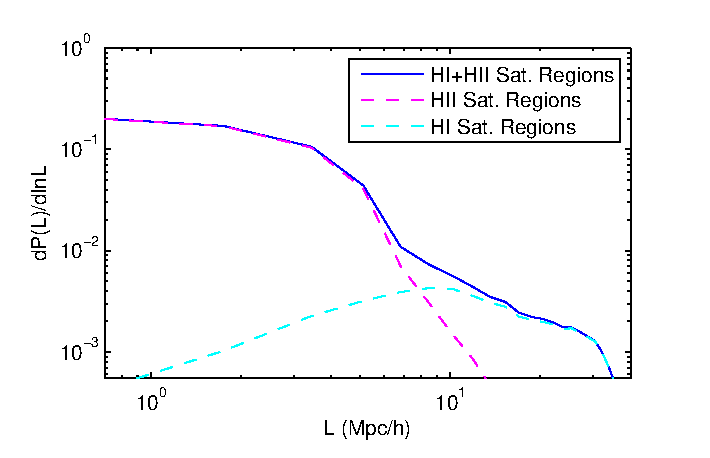
\includegraphics[width=9cm]{fig2.eps}
  \caption{Dark gap size distribution for the $\axhi = 0.22$, $\langle F \rangle = 0.1$ model. The solid blue curve shows the total distribution of dark gaps from an ensemble of mock spectra, where the magenta (cyan) curve shows the same thing but for the dark gaps sourced by ionized (neutral) gas. Here, we have focused on dark gaps with $L > 0.75 \mpch$. This clearly demonstrates that neutral hydrogen is the dominant source of {\em large} dark gaps in our mock spectra, provided there is an appreciable neutral fraction.}
  \label{fig:DarkGapHist}
\end{figure}


\begin{figure}[h]
  \centering
  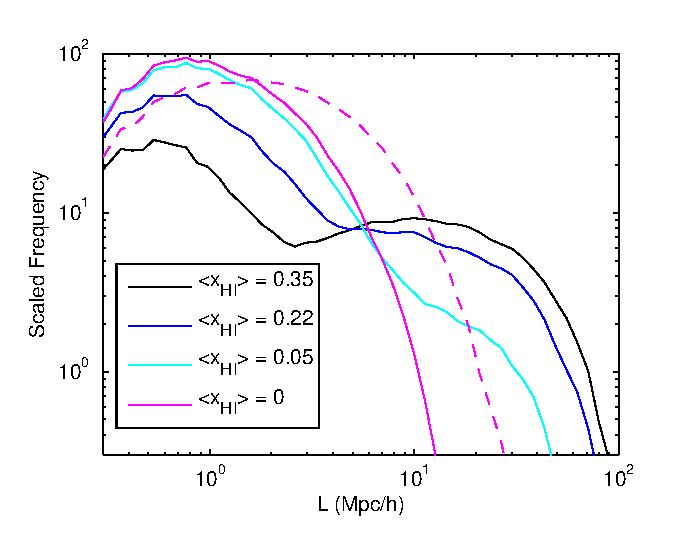
\includegraphics[width=9cm]{fig3.eps}
  \caption{Large-length tail of the dark gap size histogram for $\axhi = 0$ (magenta), 0.05 (cyan), 0.22 (blue), and 0.35 (black) for the case when $\left\langle F \right\rangle = 0.1$. The y-axis is scaled to indicate the expected number of dark gaps obtainable from 20 spectra. Bins in this figure are spaced logarithmically. The dashed magenta line indicates the dark-gap size distribution in the fully ionized case when the true transmission is $\left\langle F \right\rangle = 0.03$, but continuum fitting errors result in a measured mean transmission of $\left\langle F_{\text{meas}} \right\rangle = 0.1$.}
  \label{fig:PDFs}
\end{figure}


\section{Stacking Toy Spectra} \label{sec:Stacking}


In this section we describe our basic approach of stacking \lya\ and \lyb\ spectra in order to detect the presence of HI damping wings and absorption due to deuterium, respectively. While the forest is too absorbed at these redshifts to easily detect damping wings or deuterium absorption due to individual neutral regions, here we demonstrate that the presence of such features can be revealed \textit{on average} by stacking regions of transmission over many spectra.
 
 
This section serves as a proof of principle by applying a simplified stacking approach to mock spectra generated using an idealized IGM model. Specifically, we consider an ensemble of sightlines through our simulation box and assume that the IGM is entirely ionized with the exception of a single HI island with mean density and varying length, $L$, inserted randomly along each line of sight. We then generate mock spectra assuming these density and ionization fields. The stacking in this section is always done starting at the HI/HII boundaries of a given HI region moving outward.




\subsection{HI Damping Wing} \label{sec:ToyHI}



Our stacking approach can be clearly demonstrated by considering the damping wing from neutral hydrogen. Due to the natural width of the \lya\ line, a neutral hydrogen gas parcel should cause \lya\ absorption over a range of frequencies. Far from line center, this absorption will have an optical depth roughly following (\citealt{MiraldaEscude:1997en}):
\begin{align}
\tau_{\text{Ly}\alpha}^{\text{DW}}(\Delta v) \approx \frac{\tau_{\text{GP}}R_{\alpha}c}{\pi}\left[ \frac{1}{\Delta v} - \frac{1}{\Delta v + v_{\text{ext}}} \right]  \label{eq:HIDW}
\end{align}
where $\tau_{\text{GP}}$ is the Gunn-Paterson optical depth, $R_{\alpha} \equiv \Gamma_{\alpha}\lambda_{\alpha}/4\pi c$, $\Gamma_{\alpha} = \pow{6.265}{8}\sec^{-1}$ is the \lya\ decay constant, $\Delta v$ is the separation from the HI/HII boundary in velocity space, $v_{\text{ext}}$ is the extent of the hydrogen region in velocity space, and $c$ is the speed of light. For a large neutral region, this equation implies that $\tau^{\text{DW}}_{\text{Ly}\alpha}(|v| < 600\kms) \geq 1$ at $z \sim 5.5$. This excess absorption is referred to as the hydrogen ``damping wing". While both neutral gas and highly ionized gas can cause absorption in quasar spectra, only a significantly neutral hydrogen patch will result in damping wing absorption, owing to the greatly reduced optical depth in the wing compared to line center. As such, detecting damping wing absorption would be a smoking gun for the presence of significantly neutral hydrogen islands. Note that the transmission profile will differ from the simple form of Eq. \ref{eq:HIDW},
owing mostly to neighboring neutral regions, however the gradual recovery to transmission around saturated neutral regions should be a distinctive indicator that highly neutral regions remain in the IGM.


In \Fig{fig:ToyHI} we show the results of stacking transmission outside of neutral regions in the toy mock spectra described earlier in this section, neglecting deuterium for the time being. Namely, we show the stacked transmission outside neutral islands of length $L = 0.76 \mpch$ ($\sim 100\kms$) in black, $L = 1.27 \mpch$ ($\sim 170\kms$) in blue, $L = 5.34\mpch$ ($\sim 700\kms$) in cyan, and stacked transmission neglecting the damping wing in red. Additionally, we have plotted the analytic curves corresponding to \Eqn{eq:HIDW} for the various $L$ values, shown with dashed curves. We have applied a single multiplicative factor to these curves to account for average resonant absorption from ionized gas. Together, this figure implies that damping wing absorption from isolated neutral regions has a significant impact on quasar spectra, extending $\sim 1000\kms\ $ past the HI/HII boundaries, which may be observable through stacking as expected from Eq. \ref{eq:HIDW}. 

In providing a toy example of how the hydrogen damping wing can affect spectra, we have neglected many important challenges that such a measurement would face. For example, we assumed perfect knowledge of the underlying ionization state of the IGM in order to determine where to stack and we assumed that we could discriminate between neutral and highly ionized absorption systems. However, the presence of such a large and potentially-observable feature provides motivation for us to apply the stacking approach in a more realistic manner. In \S \ref{sec:RealSpectra} and in Appendix B, we describe several such challenges and subtleties along with potential resolutions.


\begin{figure}[h]
  \centering
  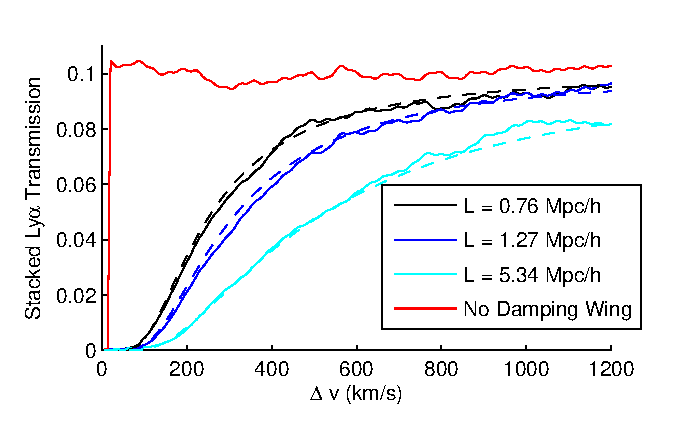
\includegraphics[width=8.4cm]{fig4.eps}
  \caption{Stacking idealized \lya\ spectra containing toy HI regions. The above figure shows the stacked transmission outside isolated HI regions with mean density and size $L = 0.76 \mpch$ ($\vext \approx 100\kms$), $L = 1.27 \mpch$ ($\vext \approx 170\kms$), and $L = 5.34 \mpch$ ($\vext \approx 700\kms$) shown in black, blue, and cyan, respectively. The solid red curve shows the stacked transmission outside of the same HI regions \textit{neglecting} the damping wing, which will be the same on average in all cases. In generating these spectra, we assume $\left\langle F \right\rangle = 0.1$. In this greatly-idealized case, the presence of the hydrogen damping wing is seen clearly through extended excess absorption compared to the red curve. Furthermore, we can see that the excess absorption closely follows what we would expect analytically based on multiplying \Eqn{eq:HIDW} by the overall mean transmission. In this figure, all stacking starts at HI/HII boundaries.}
  \label{fig:ToyHI}
\end{figure}


\subsection{Deuterium} \label{sec:ToyD}



With the stacking approach of the previous section in mind, we now consider absorption due to deuterium. As noted in \S\ref{sec:Sims}, primordial hydrogen should be accompanied by traces of deuterium, with a relative abundance of $\sim 2.5\times 10^{-5}$ (\citealt{Cooke:2013cba}). Due to its slightly increased reduced mass, atomic transitions in deuterium are shifted blueward by 82\kms\ compared to the same transitions in hydrogen. This implies that absorption due to neutral hydrogen in the IGM should be accompanied by additional absorption from deuterium, shifted blueward by 82\kms. We can estimate the optical depth for \lya\ absorption in deuterium at cosmic mean density by simply scaling the hydrogen \lya\ optical depth by the deuterium abundance:
\begin{align}
\tau_{D,\alpha} &= \left[ \frac{D}{H} \right]  \times \tau_{\text{GP}} \approx 8.25 x_{\text{HI}} \left(1+\delta\right)  \left[ \frac{1+z}{6.5} \right]^{3/2}.
\end{align}
Thus, we see that while the relative abundance of deuterium is extremely small, the Gunn-Peterson optical depth is so large that the resulting deuterium optical depth is still of order 10 in \lya.


An appealing aspect of searching for damping wing absorption is that the optical depth in the wing is large enough to cause significant absorption in the presence of neutral islands, but small enough to be negligible for ionized absorption systems. We see this again in the case of deuterium absorption, suggesting that it may be useful as an additional ``smoking gun" indicator for underlying neutral hydrogen. However, an obvious problem with detecting deuterium in \lya\ spectra is that the feature should be narrow and well within the broad range of velocities where the hydrogen damping wing is significant. Specifically, according to \Eqn{eq:HIDW}, at $\Delta v = 82\kms$, the damping wing optical depth for an extended neutral region should be $\tau_{\text{Ly}\alpha}^{\text{DW}}(\Delta v \approx 82\kms) \approx 8$. Therefore, the feature should be completely wiped out in \lya\ spectra by the hydrogen damping wing.


However, the damping wing optical depth in the \lyb\ line is much smaller. Specifically, according to \Eqn{eq:HIDW}, the damping wing optical depth scales as 
\begin{align}
\frac{\taudwb}{\taudwa} &= \frac{\tau_{\text{GP},\beta}}{\tau_{\text{GP},\alpha}} \times \frac{R_{\beta}}{R_{\alpha}} = \frac{f_{\beta}\lambda_{\beta}}{f_{\alpha}\lambda_{\alpha}} \times \frac{(\Gamma_{\beta}+\Gamma_{\text{H}\alpha})\lambda_{\beta}}{\Gamma_{\alpha}\lambda_{\alpha}} \nonumber \\
&= \dfrac{f_{\beta}^{2}}{f_{\alpha}^{2}} \left( 1 + \dfrac{f_{\text{H}\alpha}}{f_{\beta}} \dfrac{\lambda_{\beta}^2}{\lambda_{\text{H}\alpha}^2} \right) = .0410,
\end{align}
and should therefore be significantly narrower in \lyb\ than in \lya. In the above expression, $f_{\alpha}$, $f_{\beta}$, and $f_{\text{H}a}$ are the oscillator strengths of the \lya, \lyb, and Balmer-$\alpha$ transitions, respectively, with $\lambda$ denoting the corresponding wavelengths and $\Gamma$ denoting the corresponding decay constants. By modifying \Eqn{eq:HIDW} for \lyb, we see that $\taudwb(|\Delta v| \gtrsim 25\kms) \leq 1$. Therefore we find that \textit{the hydrogen damping wing should not wipe out deuterium absorption features in } \lyb. Furthermore, while the hydrogen damping wing optical depth is reduced by a factor of roughly $f_{\beta}^{2}/f_{\alpha}^{2}$ when considering \lyb, the total optical depth in the deuterium line is only reduced relative to deuterium \lya\ by $f_{\beta}\lambda_{\beta}/f_{\alpha}\lambda_{\alpha} \approx 1/6$, such that the optical depth should still be of order 1 for deuterium \lyb. Therefore, not only should a deuterium absorption feature survive the hydrogen damping wing, but it should still have a strong enough optical depth to cause significant absorption if neutral islands in fact remain.


Naturally, it should be very difficult to detect individual deuterium absorption features from the diffuse IGM, as the Ly-$\beta$ spectra will be very absorbed when the universe is neutral enough to
produce the features in the first place. However, the feature may nonetheless be observable \textit{on average} through the stacking of high-resolution quasar spectra. 
In order to demonstrate the strength of the deuterium absorption feature in stacked spectra, we incorporate deuterium into the same toy sightlines from \S \ref{sec:ToyHI} to produce mock \lyb\ spectra, neglecting foreground \lya\ absorption for the time being. We are then able to stack transmission outside of neutral regions in the spectra, starting at the HI/HII boundaries and moving outward. However, since deuterium absorption will only occur on the blue side of neutral regions, we need only stack those regions of transmission. In fact, this offers a clean test for detecting deuterium. Namely, we can separately stack transmission redward and blueward of neutral regions and compare. Excess absorption on the blue side of neutral regions, on average, could signal the presence of deuterium absorption. This is especially appealing since there should be no sources of contamination that would cause a similar, and significant, red/blue asymmetry.\footnote{One source of asymmetry we do find, which can be seen in \Fig{fig:LybResults}, results from the fact that, when dealing with realistic spectra, we force there to be transmission in \lyb\ at the locations where stacking begins. This results in a small selection effect, where selected neutral absorption systems have a reduced probability of having nearby neutral regions and have correspondingly-smaller nearby optical depths. For deuterium, this smaller optical depth is shifted blueward, causing \textit{less} absorption on the blue side of the line for $\Delta v \gtrsim 82\kms$. However, this asymmetry is minor and {\it opposes} the asymmetry from deuterium absorption.}


In \Fig{fig:ToyD}, we show the results of stacking transmission in \lyb\ redward (red) and blueward (black) of the toy neutral regions across the full ensemble of mock quasar spectra. As in \Fig{fig:ToyHI}, all stacking begins at HI/HII boundaries. We can see the blueward transmission clearly exhibits excess absorption due to deuterium extending roughly $\sim$80\kms\ from the HI/HII boundary. Thus, in this idealized scenario, the presence of deuterium in islands of neutral hydrogen leaves a very clear signature in the stacked \lyb\ transmission.

Before proceeding further, we should point out one important caveat here. In our simulated models, the transition between fully neutral and highly ionized regions is, by construction, perfectly sharp. If this
transition is more gradual in reality, then the narrow deuterium feature could be overwhelmed by absorption from mostly ionized hydrogen in this transition region. A minimal scale for this transition
region is set roughly by the mean free path to ionizing photons through the neutral IGM, which is only $\lambda_{\text{HI}} \sim 1/(n_{\text{HI}} \sigma_{\text{HI}}) \approx 6 \text{proper kpc}/h \approx 0.8 \kms$.
This minimal scale is two orders of magnitude smaller than the scale of the deuterium feature and hence does not present a worry. However, if the edges of the ionized regions tend to experience
a reduced ionizing background, this might obscure the deuterium feature, even in the case of a partly neutral IGM. We believe the possibility of detecting this deuterium feature is enticing enough to
warrant further investigation.


As was the case in \S \ref{sec:ToyHI}, we have made several simplifying assumptions and have additionally neglected foreground \lya\ absorption from the lower-redshift IGM. However, the clear presence of deuterium absorption revealed through the simplified stacking approach provides motivation to also consider applying it to more realistic spectra, as will be discussed in \S \ref{sec:RealSpectra}.


\begin{figure}[h]
  \centering
  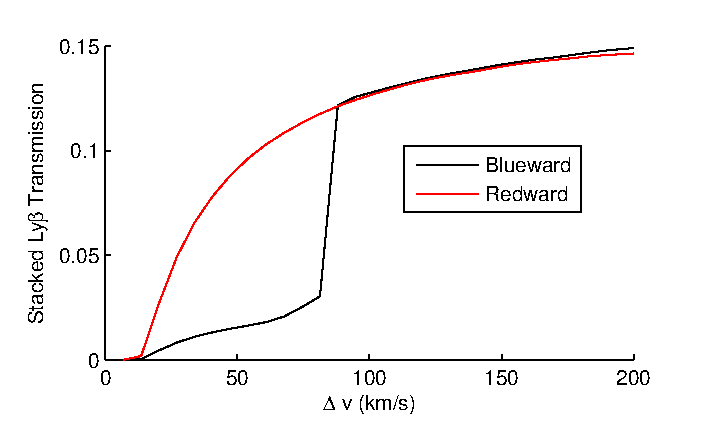
\includegraphics[width=8.4cm]{fig5.eps}
  \caption{Presence of deuterium absorption revealed through stacking idealized \lyb\ spectra containing toy neutral regions. The red and black curves show the stacked \lyb\ transmission redward and blueward, respectively, of toy neutral regions of length $L = 5\mpch$ ($\approx 700\kms$) randomly inserted into many sightlines, with spectra generated assuming $\left\langle F_{\text{Ly}\alpha} \right\rangle = 0.1$. In each case, stacking begins at the underlying HI/HII boundary. We have also mimicked the effect of including foreground \lya\ absorption by scaling the feature by the mean transmission in the foreground \lya\ forest. This demonstrates that, at least in this idealized case, the presence of deuterium absorption can be easily seen out to $\sim80\kms$\ past the HI/HII boundaries.}
  \label{fig:ToyD}
\end{figure}




\section{Steps of Approach} \label{sec:RealSpectra}


In \S\ref{sec:Stacking}, we demonstrated the utility of stacking idealized quasar spectra in order to reveal the presence of the HI damping wing and deuterium absorption. The success of this approach in the toy case provides motivation for us to apply it to realistic mock spectra. In doing so, we must confront the simplifying assumptions made in \S\ref{sec:Stacking}. 


The most obviously unrealistic assumption made in \S\ref{sec:Stacking} is that we can precisely identify the HI/HII boundaries underlying our spectra. In practice, we will only have access to the level of transmission at each point along the spectra. However, based on \Fig{fig:ToyD}, the recovery from saturated absorption to transmission occurs within $\lesssim 15\kms$ in \lyb\ from the edge of the neutral zone, and should therefore provide a relatively
good indicator of the HI/HII boundary. Therefore, we choose to identify stacking locations based on where transmission recovers \textit{in \lyb}.
To be clear, for the case of the hydrogen damping wing, we are stacking transmission in the \lya\ forest, but we are choosing where to start the stacking based on features in the \lyb\ forest. A drawback of this approach, when searching for the hydrogen damping wing, is that we are only able to stack regions of the \lya\ forest with corresponding regions in the \lyb\ forest that are not contaminated by \lyc\ absorption. This effectively reduces the amount of usable spectra, since, for a quasar at $z = 5.5$, the pure \lya\ forest will extend $4.5 \leq z \leq 5.5$, but \lyc\ absorption will contaminate the \lyb\ forest at $z \lesssim 5.16$. If presented with a limited number of spectra, it may be worth searching for the damping wing by using only the \lya\ regions of the spectra. 


By stacking at the precise locations of HI/HII boundaries in \S\ref{sec:Stacking}, we were also ensuring that our sample of absorption systems was all neutral. However, when we modify our approach to begin stacking at locations where transmission recovers from saturated absorption, we may start stacking transmission outside of ionized absorption systems together with transmission outside of neutral absorption systems, diluting our signal. Since the signal we are aiming to find is small to begin with, it is important that we minimize this contamination from ionized regions. To do this, we take advantage of the main argument of \S\ref{sec:HIDistributions}, namely that regions of saturated absorption sourced by neutral gas should be significantly larger, on average, than those sourced by ionized gas. Therefore, we choose to stack only transmission outside of \textit{large} regions of saturated absorption. Furthermore, since true neutral regions should cause saturated absorption in \lyb, we choose to stack only outside of large saturated regions which are fully absorbed in \lyb, where we define ``large" to be $>500\kms\ $ ($\gtrsim 4\mpch$) in \lyb. Note that this choice is tuned for
the case of $\avg{F} = 0.1$: a different choice may be better for other values of the mean transmitted flux. At any rate, in applying these tests to real data, one would likely vary this size scale across a range
of possible values.


Additionally, an appealing feature of the search for deuterium absorption is that it offers a very clean test for its detection, namely a red/blue asymmetry in the transmission outside of plausibly neutral regions. The disparity in the size distribution of saturated regions sourced by neutral and ionized gas suggests a similar test may be possible for the detection of the HI damping wing. Namely, while large regions of saturated absorption are likely to be sourced by neutral gas, small regions of saturated absorption are likely to be sourced by ionized gas. Therefore, to find evidence of excess absorption outside of neutral regions due to the HI damping wing, we compare the stacked transmission outside of large absorption systems, plausibly sourced by neutral gas, to that outside of small absorption systems, likely sourced by ionized gas. A significant amount of excess absorption outside of the former compared to the latter, extending further than any possible density correlations, would suggest the presence of damping wing absorption.


Furthermore, in \S\ref{sec:ToyD}, we discussed how the damping wing is greatly weakened in \lyb\ compared to in \lya. Therefore, an additional test for the presence of damping wing absorption could be to take the ratio of the stacked \lyb\ transmission to the stacked \lya\ transmission, where stacking occurs in the same physical regions in both cases. In the event that there is significant damping wing absorption, this ratio should also slowly recover to some constant value at large $\Delta v$. We further discuss and develop this approach in Appendix B.


When dealing with realistic spectra, we must adjust our approach to accommodate the presence of noise (and finite spectral resolution). While noise should average out in stacked regions, the presence of noise will also obfuscate the precise boundaries between saturated absorption and transmission. We choose to handle this by smoothing our noisy spectra over a scale of 100 km/s ($\sim 0.75\mpch$) and defining any pixel, $i$, with transmission $F_i < 3\tilde{\sigma}_{\text{N}}$ to be consistent with saturated absorption, where $\tilde{\sigma}_{\text{N}}$ denotes the standard deviation of the smoothed noise. We then define regions in the smoothed spectra where the flux goes from $F<3\tilde{\sigma}_{\text{N}}$ to $F>3\tilde{\sigma}_{\text{N}}$ as the transitions from saturated absorption to transmission, and therefore as potential points to start stacking. When stacking transmission, however, we stack the transmission in the \textit{unsmoothed} spectra.

Another concern is that damping wing absorption sourced by DLAs may erroneously be attributed to a significantly neutral IGM. However, in Appendix A, we estimate the expected rate of DLAs occurring in $z \sim 5.5$ quasar spectra and find it is small enough to be ignored. Additionally, DLAs may be discriminated from diffuse neutral islands based on the presence of metal lines and the relative sizes of their absorption in \lya\ and \lyb. 

Finally, as mentioned previously, we approximate the ionizing background in the ionized regions as uniform and ignore scatter in the temperature density relation. Accounting for these fluctuations {\em might}
lead to a more gradual recovery in the transmission around absorbed regions -- in the case of a fully ionized universe -- than in our models. Further investigation of this issue would certainly be required if a gradual recovery
is indeed found in real spectra. In Appendix B, we discuss a possible empirical test that may help in this regard.



\section{Results} \label{sec:Results}


Having considered the subtleties of the previous section, we are now ready to apply the three-pronged approach to more realistic mock spectra. In each section, we first consider the ideal case where no noise has been applied to give an idea of the potential constraining power of the different methods. Subsequently, we add realistic levels of noise and consider realistic spectra resolution to give an idea of the constraining power of the approaches applied to Keck HIRES spectra for the deuterium feature and damping wing, and spectra with slightly higher resolution than SDSS for the dark gap size distribution.


\subsection{Detecting the Damping Wing} \label{sec:Damping Wing Results}



We first consider the ability to uncover the presence of the hydrogen damping wing by strategically stacking regions of transmission in the the \lya\ forest of $z \approx 5.5$ noiseless mock quasar spectra. As discussed in \S \ref{sec:RealSpectra}, our aim is to compare the average transmission outside of plausibly neutral absorption systems to the transmission outside of likely ionized systems. 


We identify the plausibly neutral absorption systems by requiring the regions be completely absorbed in \lyb, and also that the regions of saturated absorption are at least $L_{\text{sat}} > 500\kms$ ($\sim4\mpch$) \textit{in \lyb}. We begin stacking at the point in the \lya\ spectrum which corresponds to the recovery from absorption to transmission \textit{in \lyb}. We identify the likely ionized absorption systems by requiring that they are \textit{below} a maximum length $L_{\text{max}} = 300\kms$ \textit{in \lyb}.


In \Fig{fig:LyaResults}, we show the results of applying this approach to realistic mock spectra generated assuming various ionization states of the IGM. In the top panel, we show the stacked transmission outside of plausibly neutral absorption systems (solid) and likely ionized absorption systems (dashed), using a volume-averaged neutral fraction of $\axhi = 0.35$ (black), 0.22 (blue), 0.05 (cyan), and $\axhi = 0$ (magenta). The curves agree with our expectations, namely that transmission outside of neutral regions should recover more slowly and exhibit a rough damping wing shape with a large extent in velocity space. We see that the excess absorption extends \textit{farther} than the $\lesssim 1000\kms\ $expected from an isolated damping wing. However, as discussed in Appendix C, we find that the spatial clustering of neutral regions is responsible for this effect. 


While, for several reasons discussed earlier, the shape of the absorption is distorted compared to \Fig{fig:ToyHI}, it can be seen for all significantly neutral ionization states. An important check is to apply the stacking procedure to a fully ionized IGM and ensure that we do not make a false detection. The results of this check are shown by the magenta curves in \Fig{fig:LyaResults}. As we can see, the resulting stacked transmission outside of plausibly neutral regions lacks an overall damping wing shape and stays roughly fixed near the mean transmission. 


We can also see that the transmission outside of small absorption systems is very sensitive to the underlying neutral fraction. We expect this, however, since this stacked transmission depends strongly on the average transmission in regions which are not in saturated absorption, denoted $\langle F | F > 0 \rangle$. Since the dark pixel covering fraction in our mock spectra increases with $\axhi$, mock spectra with larger neutral fractions must have larger values for $\langle F | F > 0 \rangle$ to maintain $\langle F \rangle = 0.1$. As such, \Fig{fig:LyaResults} shows that the stacked transmission outside of small absorption systems increases monotonically with $\axhi$. 


We estimated the stacked transmission from a large ensemble of simulated spectra to produce a smooth estimate of the average transmission around saturated regions in each model.
The transmission curves outside of individual absorption systems are, however, quite noisy on their own such that, from saturated region to saturated region, there is significant scatter about the mean-value curves shown in the top panel. In order to estimate how confidently we can distinguish the solid and dashed curves with a reasonable number of quasar spectra, we scale the number of identified absorption systems to what we would expect using $\sim 20$ spectra. Specifically, we take the difference between the dashed and solid curves and divide by the scatter in each bin. The scatter of each bin is simply the scatter in stacked transmission outside of large absorption systems, scaled by $1/\sqrt{N_{\text{sat,large}}}$, added in quadrature with the scatter in the stacked transmission outside of small absorption systems, scaled by $1/\sqrt{N_{\text{sat,small}}}$.  Here we scale to estimate the plausible scatter around the mean after estimating the transmission around saturated regions using $20$ quasar absorption
spectra.


The results of this are shown in the bottom panel of \Fig{fig:LyaResults} for the same ionization states. The results appear to be very encouraging, indicating that, assuming noiseless spectra, the solid and dashed curves are $\gtrsim 5\sigma$ statistically-significantly different (\textit{even for $\axhi = 0.05$!}). In addition, we see that the difference roughly follows a damping wing shape and remains significant for $\gtrsim 3000\kms$. We should emphasize that, while the deuterium absorption feature will necessarily be a $\lesssim 80\kms\ $ feature and require high resolution spectra to be seen, the damping wing feature extends an order of magnitude farther in velocity space and should be accessible to lower-resolution spectra. 


In \Fig{fig:LyaResults_LowF}, we show the same results as in \Fig{fig:LyaResults}, but assume a lower mean transmission of $\left\langle F \right\rangle = 0.05$, consistent with spectra at $5.7 \lesssim z < 6$ (\citealt{Becker:2001ee}). From the figure, we see that these results are very similar to those for $\left\langle F \right\rangle = 0.10$, but with the significance curves peaking at a $\sim 70\%$ lower value and with the stacked transmission recovering to a lower mean. Overall, this provides encouragement for applying the approach to higher-$z$ spectra, suggesting that a range of physically interesting neutral fractions could be probed.


It is also interesting to consider these results when spectra are generated according to the specifications of existing data. In \Fig{fig:HIRES_LyaResults_Noisy} we show the same results as in the bottom panel of \Fig{fig:LyaResults} except we have adjusted the spectra to mimic HIRES spectra. Namely, we have assumed a spectral resolution with $\text{FWHM} = 6.7\kms\ $ and bins with size $\Delta v_{\text{bin}} = 2.1\kms$ (e.g. \citealt{Viel:2013fqw}). Additionally, we have assumed a signal to noise of $\text{SNR} = 10$ at the continuum per $2.1\kms\ $ pixel and that we have 20 such spectra. While we are currently only aware of 10 such spectra, this case is still interesting since spectra with significantly worse spectral resolution should also be adequate for this test. 


From this figure, we can see that, despite the degradation of the spectra, the damping wing is still visible with the significance curve peaking at $\gtrsim 5\sigma$ ($\gtrsim 8\sigma$) significance for the $\axhi = 0.22$ ($0.35$) ionization state. However, this figure suggests that, in the $\axhi = 0.05$ case, it is less-clear whether the damping wing is detectable. 



An important effect of adding noise to the mock spectra is that it obscures the precise location where spectra should be stacked and also increases the fraction of selected saturated regions which are, in fact, ionized. We find that for the spectra in this section $\sim 30\%$, 40\%, and 75\% of identified plausibly neutral regions are in in fact ionized for $\axhi = 0.35$, 0.22, and 0.05, respectively. This is compared to $\sim 7\%$, 10\%, and 20\% contamination when noise is neglected.


Statistical significances in this section are only estimates. In reality, the statistical significance with which the damping wing can be detected will depend on how extended the significance curves are, along with how correlated the errors in neighboring bins are. We discuss this in \S\ref{sec:Forecasts}.


\begin{figure}[h]
  \centering
  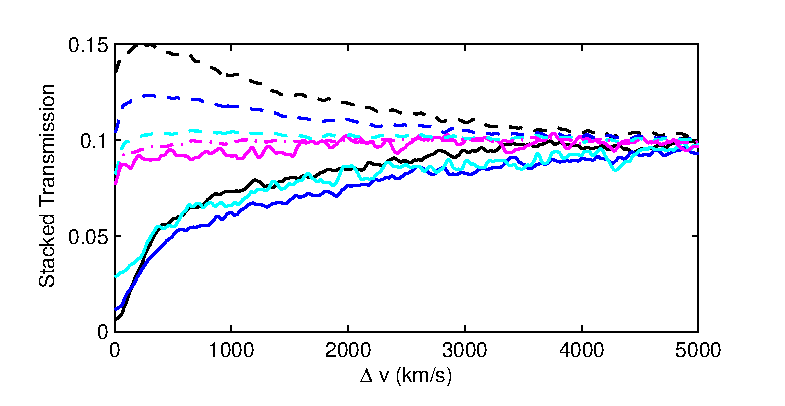
\includegraphics[width=9cm]{fig6a.eps}
  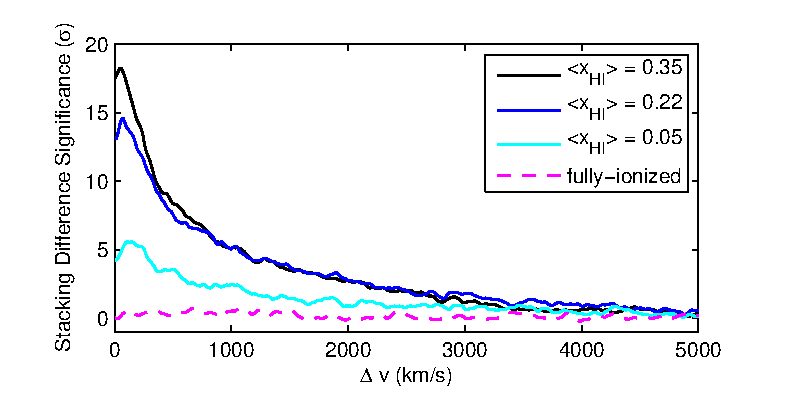
\includegraphics[width=9cm]{fig6b.eps}
  \caption{\lya\ stacking results for various neutral fractions. The top panel shows the mean (noiseless) stacked transmission outside of large absorption systems (solid) and small absorption systems (dashed) in the \lya\ forest for neutral fractions $\axhi = 0.35$ (black), 0.22 (blue), 0.05 (red), and 0 (magenta). The transmission here is estimated from a large ensemble of mock spectra to obtain a smooth estimate
  of the average transmission around saturated regions in each model. 
  The bottom panel shows the statistical significance of the difference between the dashed and solid curves in the top panel assuming a sample of 20 spectra are used in the stacking process.}
  \label{fig:LyaResults}
\end{figure}


\begin{figure}[h]
  \centering
  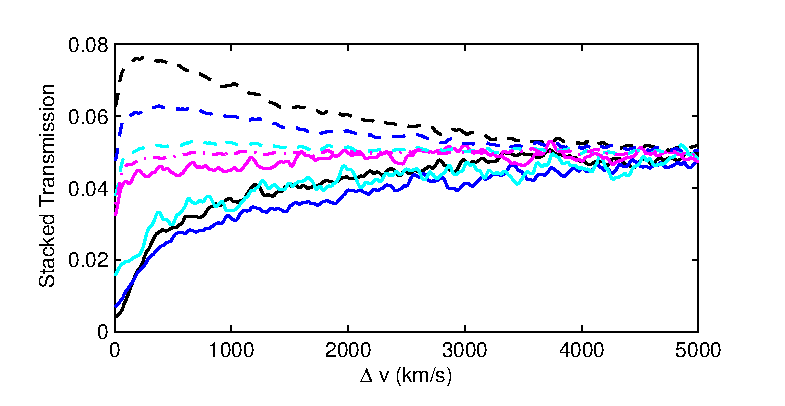
\includegraphics[width=9cm]{fig7a.eps}
  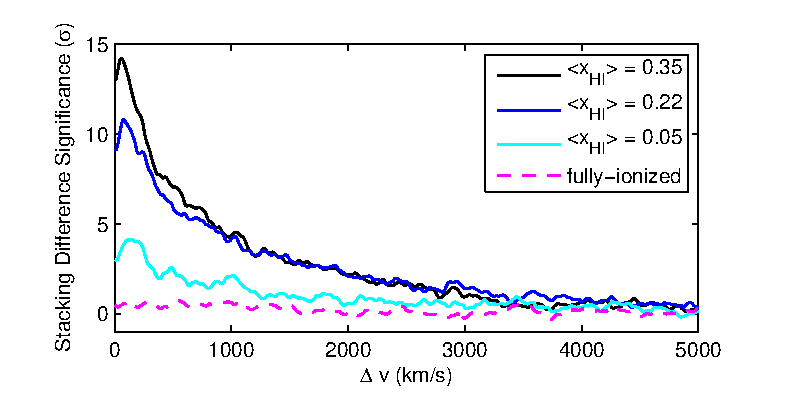
\includegraphics[width=9cm]{fig7b.eps}
  \caption{\lya\ stacking results assuming $\left\langle F \right\rangle = 0.05$. The above panels are identical to those in \Fig{fig:LyaResults} except that mock spectra have been generated assuming $\left\langle F \right\rangle = 0.05$. }
  \label{fig:LyaResults_LowF}
\end{figure}


\begin{figure}[h]
  \centering
  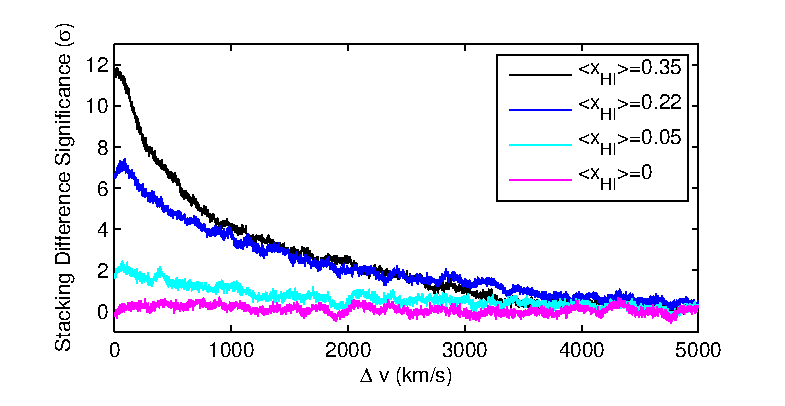
\includegraphics[width=9cm]{fig8.eps}
  \caption{Results of \lya\ stacking with HIRES-style spectra ($\left\langle F \right\rangle = 0.1$). The above panel is identical to the bottom panel in \Fig{fig:LyaResults} except that the spectra have had the bin size and spectral resolution adjusted to match that of Keck-HIRES spectra. Additionally, we have added noise such that the spectra have a signal-to-noise value of 10 per pixel at the continuum.}
  \label{fig:HIRES_LyaResults_Noisy}
\end{figure}


\subsection{Deuterium Feature Results} \label{sec:DeuteriumResults}


We now turn to consider the prospects for identifying deuterium absorption in realistic \lyb\ mock spectra. As discussed in \S \ref{sec:RealSpectra}, our aim is to identify plausibly neutral absorption systems in the \lyb\ spectra and compare the stacked transmission moving blueward and redward away from the absorption. We identify the plausibly neutral regions in the same manner as for the damping wing.

In \Fig{fig:LybResults}, we show the results of applying the stacking approach to the same mock spectra as in the previous section. The top panel shows the mean transmission blueward (solid) and redward (dashed) moving away from plausibly neutral absorption systems for the same ionization states as in the previous section. We can very clearly see excess absorption in the partially neutral spectra, extending $\sim 80\kms$, consistent with our expectations from \Fig{fig:ToyD}. Additionally, we also find that, in the fully ionized case, the blueward and redward stacked transmission match up very well. 


As in the previous section, we can construct a rough significance curve for the difference between the blueward and redward transmission. Specifically, in the bottom panel of \Fig{fig:LybResults} we show the excess blueward absorption in units of the standard deviation of the stacked blueward transmission assuming 20 quasar spectra. We can see that the significance of the red/blue asymmetry extends $\sim 70\kms$ ($\sim 0.3 \mpch$) and is $\gtrsim 3\sigma$ for all of the partially neutral models considered, with increasing significance for models with higher neutral fractions. Additionally, we see that the curve corresponding to the fully ionized model shows no statistically-significant deviation from red/blue symmetry. Thus, this is indeed a very clean test for the presence of deuterium. However, the signal itself is an order of magnitude smaller in velocity-space extent and is found with significantly less statistical significance than the damping wing signal. Therefore, we expect that high-resolution, high-signal-to-noise spectra will be necessary to search for it. 


As in \S\ref{sec:Damping Wing Results}, we can reproduce \Fig{fig:LybResults} assuming spectra with specifications mimicking Keck HIRES. Unfortunately, we find that, with a signal to noise per pixel in the continuum of 10, the deuterium feature is hard to observe. Because of this, we consider using 20 HIRES-style spectra with a signal to noise per pixel of 30 in the continuum. While this signal-to-noise value is higher than those for existing spectra we found in the literature, it is not unreasonable to assume such spectra may become available in the future. Furthermore, this may provide additional motivation to obtain such spectra. Regardless, after applying the stacking approach with twenty $\text{SNR} = 30$ HIRES spectra, we obtain the results shown in \Fig{fig:LybResults_Noisy}. This figure shows that the feature should be observable with modest statistical significance. Specifically, for $\xhi = 0.35$ (0.22) the significance curve peaks at $\sim 3.7\sigma$ ($\sim 3\sigma$). Additionally, when these curves are generated assuming MIKE-style spectra, with spectral resolution $\text{FWHM} = 13.6\kms\ $ and velocity bin size $\Delta v_{\text{bin}} = 5.0\kms$, we obtain similar curves as in \Fig{fig:LybResults_Noisy} but with the signal being statistically significant over a smaller range of velocities. 


Again, important effects of adding noise to the mock spectra are that it obscures the precise location where spectra should be stacked and increases the fraction of selected plausibly neutral regions which are, in fact, ionized. We find that for the spectra in this section $\sim 15\%$, 20\%, and 40\% of identified plausibly neutral regions are in in fact ionized for $\axhi = 0.35$, 0.22, and 0.05, respectively. This is compared to $\sim 7\%$, 10\%, and 20\% contamination when noise is neglected. As expected, we find a smaller level of contamination than in the previous section, owing to the increased signal to noise of the spectra used. However, for the case of deuterium, the effect of noise on the stacking location is more apparent. \Fig{fig:LybResults} demonstrates that, without noise, deuterium absorption imprints a feature on stacked noiseless spectra extending $\approx 80\kms$, but only extending $\approx 60\kms\ $ in stacked noisy spectra, as shown in \Fig{fig:LybResults_Noisy}.


The above results suggest that stacking \lyb\ transmission in high-$z$ spectra can indeed be used to detect the presence of primordial deuterium, and hence that of hydrogen, but that high-resolution and high signal-to-noise spectra will be required. Nevertheless, it would certainly be interesting to apply this approach to existing HIRES/MIKE spectra as it provides an additional test, independent of the damping wing search, for the presence of underlying neutral hydrogen in the IGM. As such, a detection with modest levels of statistical significance could lend credence to a claimed detection of the HI damping wing. 


\begin{figure}[t]
  \centering
  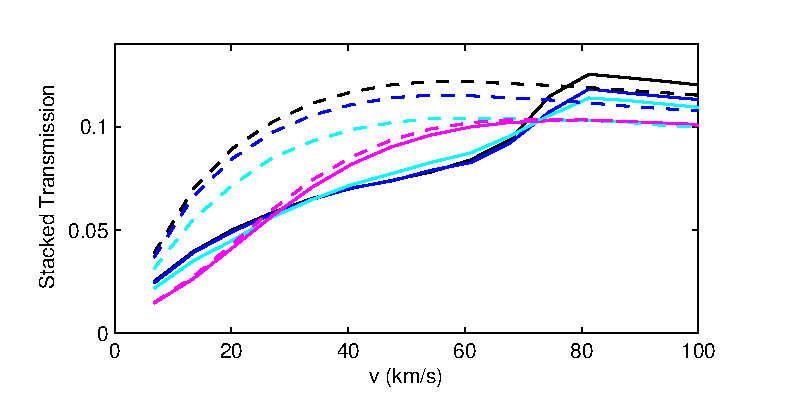
\includegraphics[width=9cm]{fig9a.eps}
  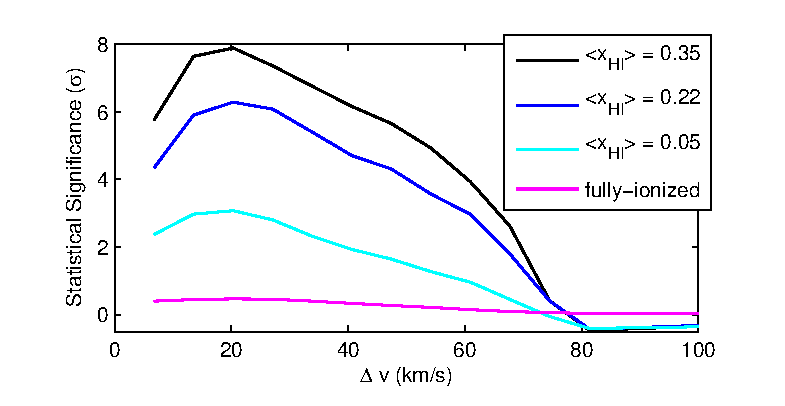
\includegraphics[width=9cm]{fig9b.eps}
  \caption{Deuterium \lyb\ stacking results for various neutral fractions. The top panel shows the mean ensemble-averaged noiseless stacked transmission moving blueward (solid) and redward (dashed) away from large absorption systems in the \lyb\ forest for neutral fractions $\axhi = 0.35$ (black), 0.22 (blue), 0.05 (cyan), and 0 (magenta). The bottom panel shows the excess blueward absorption in units of the standard deviation of the stacked redward transmission, assuming 20 spectra. }
  \label{fig:LybResults}
\end{figure}

\begin{figure}[h]
  \centering
  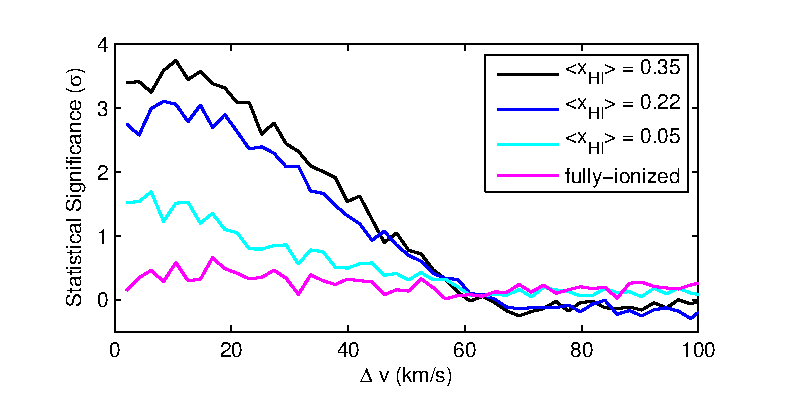
\includegraphics[width=9cm]{fig10.eps}
  \caption{Results of \lyb\ stacking with HIRES-style spectra. The above panel is the same as in the bottom panel of \Fig{fig:LybResults}, except that it is generated using HIRES-style spectra, with spectral resolution of $\text{FWHM}=6.7\kms\ $ and additive noise with signal to noise of 30 per 2.1 km/s pixel at the continuum. }
  \label{fig:LybResults_Noisy}
\end{figure}




\subsection{Dark Gap Statistics} \label{sec:DarkGaps}


We now shift our focus away from stacking and toward the distribution in lengths of regions of saturated absorption (dark gaps). As discussed in \S\ref{sec:HIDistributions}, the dark gap size distribution in quasar spectra should contain information about the underlying ionization state of the IGM. Specifically, in a more neutral IGM, the typical sizes of dark gaps should be larger and the shape of the dark gap size distribution should have a more gradual decline, and possibly show a hint of bimodality, toward large $L$. 


We continue this discussion in this section by considering plausible dark gap size distributions that could be observed with moderate-resolution, moderate-signal-to-noise spectra. Specifically, we consider spectra with spectral resolution $\text{FWHM} = 100\kms$, bin size $v_{\text{bin}} = 50\kms$, and a signal-to-noise ratio of 10 at the continuum. These spectra are of only slightly better quality than SDSS spectra. Additionally, since we are not concerned with \lyb\ transmission, we are able to use the entire \lya\ forest for each spectra.



In \Fig{fig:DarkGapsResults}, we show the resulting dark gap size histogram expected for 20 such spectra for $\axhi = 0.35$ (black), 0.22 (blue), 0.05 (cyan), and 0 (magenta). In generating this figure, we use the same ensemble of mock spectra as in \S\ref{sec:Damping Wing Results} and \S\ref{sec:DeuteriumResults}, except with their spectral resolution and bin size modified as mentioned. We maintain the requirement that $\left\langle F \right\rangle = 0.1$. 


This figure qualitatively agrees with \Fig{fig:PDFs}, where noiseless spectra with finer spectral resolution were used, but shows a shift toward larger $L$ due to smoothing the spectra. Additionally, the ionization states are not as easily distinguishable as in \Fig{fig:PDFs}, with the $\axhi = 0.05$ distribution looking practically identical to the fully ionized scenario. However, for the other neutral fractions considered, the situation looks very encouraging. The distributions for $\axhi = 0.22$ and 0.35 show a more gradual decline toward large $L$ than the fully ionized case and also reveal the clear emergence of a bimodal distribution. Additionally, the largest dark gaps in these ionization states are roughly twice as large as in the fully ionized case. 


\begin{figure}[h]
  \centering
  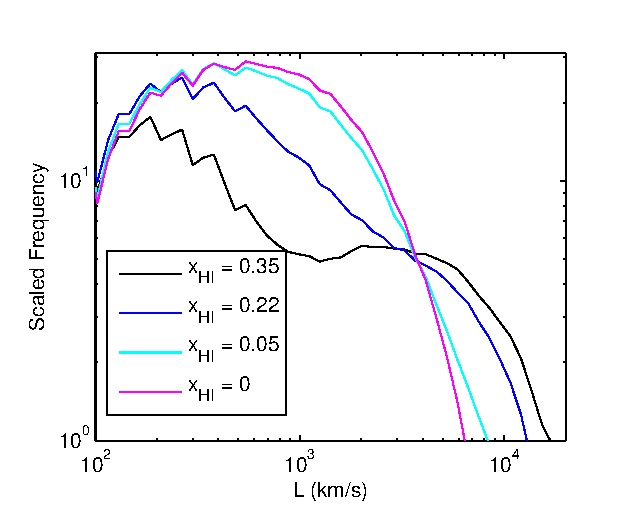
\includegraphics[width=8.5cm]{fig11.eps}
  \caption{Mock dark gap size distribution. This figure is identical to \Fig{fig:PDFs} except that it uses spectra with spectral resolution $\text{FWHM} = 100\kms$, bin size $\Delta v_{\text{bin}} = 50\kms$, and a signal-to-noise ratio of 10 at the continuum. This figure shows the expected histogram of dark gap sizes using 20 spectra with $\axhi = 0.35$ (black), 0.22 (blue), 0.05 (cyan), and 0 (magenta) at fixed $\left\langle F \right\rangle = 0.1$.}
  \label{fig:DarkGapsResults}
\end{figure}



\section{Forecasts} \label{sec:Forecasts}


Having discussed the results of the proposed stacking approaches applied to realistic mock spectra, we now consider the ability of these methods to constrain the ionization state of the $z \sim 5.5$ IGM. Specifically, in this section we focus on the ability of each method to rule out the hypothesis of a fully ionized IGM. 


In both the case of the HI damping wing and deuterium absorption feature, we would like to compare models representing different ionization states and estimate the $\Delta \chi^2$ between $\axhi \neq 0$ models and the fully ionized model, assuming a reasonable number of spectra. Let $F_{\axhi}(\Delta v)$ denote the mean behavior for a model with given neutral fraction, $\axhi$, as a function of stacked velocity separation and let $F_{\text{ion}}(\Delta v)$ denote the mean behavior of the ionized model, also as a function of stacked velocity separation. The precise definitions of what is meant by behavior will be discussed later in this section. In this case, the $\Delta \chi^2$ value between two models can be calculated by
\begin{align}
\Delta \chi^2_{\axhi} &= \Delta F_{\axhi} \cdot C^{-1} \cdot \Delta F_{\axhi}^{\text{T}} \label{eq:ChiSquare}
\end{align}
where $C$ is the covariance matrix of the $\axhi$ model, representing the correlation between stacked pixels, and $\Delta F_{\axhi}(\Delta v) \equiv F_{\text{ion}}(\Delta v) - F_{\axhi}(\Delta v)$, with $\Delta F_{\axhi}^{\text{T}}$ denoting its transpose. For simplicity, rather than estimating the full covariance matrix and its inverse, we approximate pixels at sufficiently wide separations as independent. We
then coarsely sample the pixels -- on the scale where they can be well approximated as independent -- and assume a diagonal covariance matrix for the coarsely sampled pixels. Specifically,
we estimate  $\Delta \chi^{2}_{\axhi}$ by simply adding up the squared statistical significance of each coarsely-sampled bin, $\left[\Delta F_{\axhi}(\Delta v_i)/\sigma_{\axhi}(\Delta v_i)\right]^2$, where $\sigma_{\axhi}(\Delta v_i)$ is the standard deviation of $F_{\axhi}(\Delta v_i)$. 




\subsection{Deuterium} \label{sec:DForecast}

 Perhaps it is best to consider the case of the deuterium absorption feature first. In the case of a fully ionized IGM, the transmission looking blueward and redward from absorption systems should be symmetric on average, with excess blueward absorption only occurring when the IGM is significantly neutral. Therefore, we may calculate the $\Delta \chi_{\axhi}^2$ between stacked transmission looking redward ($F_{\axhi,\text{red}}(v)$) and blueward ($F_{\axhi,\text{blue}}(v)$) from plausibly neutral absorption systems for each ionization state $\axhi$ to estimate our ability to rule out the hypothesis of a fully ionized IGM in each case. 
 
 
Thus, in the context of \Eqn{eq:ChiSquare}, we have 
\begin{align}
\Delta F_{\axhi}(\Delta v) &\equiv F_{\axhi,\text{red}}(\Delta v) - F_{\axhi,\text{blue}}(\Delta v) \\
C^{-1}_{ij} &= \delta_{ij} /\sigma^2_{\axhi,\text{blue}}(v_i)
\end{align}
where $\sigma_{\axhi,\text{blue}}(v_i)$ is the standard deviation of the stacked transmission blueward of plausibly neutral absorption systems, assuming a given number of spectra, and we have assumed that we have already resampled $\Delta F_{\axhi}(v)$ at sufficient velocity separations such that neighboring bins can be approximated as independent. At this point, the only missing ingredient is the minimum separation between two stacked pixels for them to be considered independent. We calculate the correlation function between stacked pixels in \lyb, and find that the correlation has a width of $\text{FWHM} \approx 80\kms$ and, as such, we do not expect to get more than one independent bin within the scale of the deuterium feature. Therefore, a rough estimate of the $\Delta \chi^2_{\axhi}$ value obtainable in each ionization state can be estimated simply by the peak value in the ``significance curves" in \Fig{fig:LybResults_Noisy}. Thus, if the underlying neutral fraction of the IGM is $\axhi = 0.22$ (0.35), then we expect to be able to rule out a fully ionized IGM with $\sim3\sigma$ ($\sim 3.7 \sigma$) confidence, assuming 20 HIRES/MIKE spectra with signal to noise of 30 per pixel at the continuum. Unfortunately, we do not expect to be able to rule out the hypothesis of a fully ionized IGM if the underlying neutral fraction is $\axhi \lesssim 0.05$.



\subsection{HI Damping Wing} \label{sec:HIForecast}

 
 Assessing the statistical significance with which we can observe the HI damping wing is slightly more complicated than the deuterium case since the test for its detection is not as simple. When faced with actual spectra, we would look for the presence of significant and extended absorption outside of large absorption systems compared to that outside of small absorption systems. 

Therefore, the behavior we would like to compare in each case is the stacked transmission outside of plausibly neutral absorption systems ($f_{\text{large}}(\Delta v)$) and the transmission outside of likely ionized absorption systems ($f_{\text{small}}(\Delta v)$). Let us denote 
\begin{align}
F(\Delta v) &\equiv f_{\text{small}}(\Delta v) - f_{\text{large}}(\Delta v)
 \end{align}
as the difference in these stacked transmissions where $F_{\axhi}(\Delta v)$ and $F_{\text{ion}}(\Delta v)$ represent this behavior for the ionization state with neutral fraction $\axhi$ and the fully ionized state, respectively. Thus, in the context of \Eqn{eq:ChiSquare}, we have
\begin{align}
\Delta F_{\axhi}(\Delta v) &= F_{\text{ion}}(\Delta v) - F_{\axhi}(\Delta v) \\
C^{-1}_{ij} &= \delta_{ij}/\sigma^2_{F_{\axhi}}(v_i) \label{eq:ChiSquare_HI}
\end{align}
 where $\sigma_{F_{\axhi}}(v_i)$ denotes the standard deviation of $F_{\axhi}(v)$ at $v_i$. The resulting $\sqrt{\Delta \chi^2}$ value indicates the expected significance with which we could rule out a \textit{fully ionized} IGM if the neutral fraction were, in fact, $\axhi$. Again, for \Eqn{eq:ChiSquare_HI}, we have assumed that $\Delta F_{\axhi}(\Delta v)$ has been resampled at velocity separations such that the pixels can be treated as independent. We find that the correlation function between pixels of stacked transmission in the \lya\ forest within the scale of the HI damping wing has $\text{FWHM}\approx 100\kms$. While this scale is large, the excess absorption due to the presence of damping wing absorption leaves a feature extending $\gtrsim 3000\kms$, leaving us with $\gtrsim 30$ independent bins within the scale of the feature.
 

In this manner, we are able to calculate a rough estimate for the $\Delta \chi^2$ values for the ionization states considered thus far.  Assuming the same type of spectra as in \Fig{fig:LyaResults}, namely 20 HIRES spectra with signal to noise in the continuum of 10 per pixel, we find that if the IGM is, in fact, $5\%$, $22\%$, or $35\%$ neutral, then we should be able to rule out a fully ionized IGM at $5.3\sigma$, $19.2\sigma$, or $26.3\sigma$, respectively. In the case of $\left\langle F \right\rangle = 0.05$, this reduces to $14.8\sigma$, $8.7\sigma$, and $2.2\sigma$, respectively.\footnotemark\  While we are only aware of $\sim 10$ such spectra that exist at the moment, we still regard this estimate as somewhat conservative. We found that excess stacked absorption due to the damping wing extends thousands of $\kms$, and therefore it is not necessary to have the state-of-the-art in spectral resolution to measure it. Especially with such extended correlation among neighboring pixels, it is unclear how much is gained by resolution improvements beyond $\sim 100\kms$.



\section{Conclusion} \label{sec:Conclusion}


In this work, we developed empirical tests of the possibility that the Epoch of Reionization is not yet complete by $z \sim 5.5$. Specifically, we proposed three measurements that can be made with existing, and future, high-redshift quasar spectra in order to investigate this region of reionization history parameter space. 


First, we discussed using the dark gap size distribution in quasar spectra as a means of constraining the $z \sim 5.5$ neutral fraction. We find that not only do the typical sizes of dark gaps increase with neutral fraction but that the \textit{shape} of the size distribution is also sensitive to the neutral fraction. Specifically, the presence of dark gaps sourced by significantly neutral hydrogen islands introduces a bimodality in the dark gap size distribution. We find that this bimodality should be observable at $z \sim 5.5$, provided that $\axhi \gtrsim 0.2$, and should not be affected by continuum fitting errors. 


Next, we proposed a method for searching for hydrogen damping wing absorption by strategically stacking regions of transmission in the \lya\ forest. Specifically, we searched for excess absorption in stacked transmission outside of plausibly neutral regions compared to that outside of likely ionized regions. We found that the presence of the hydrogen damping wing will result in excess absorption extending $\sim 5000\kms\ $ past ionization boundaries of neutral regions. Furthermore, this excess absorption should be detectable with $\gtrsim 5.3\sigma$ statistical significance for $\axhi \gtrsim 0.05$, using 20 HIRES-style spectra with a signal-to-noise value per pixel of 10 at the continuum. 


Lastly, we proposed a similar stacking measurement utilizing the \lyb\ forest in order to search for deuterium absorption associated with significantly neutral hydrogen islands at $z \sim 5.5$. We proposed searching for this feature by looking for excess absorption in stacked \lyb\ transmission blueward of plausibly neutral regions compared to the corresponding redward transmission. We find that this feature should be observable in principle but will likely require additional high-resolution spectra in order to be detected. Specifically, we find that the feature should be observable at $z \sim 5.5$ with $\sim3\sigma$ ($\sim 3.7\sigma$) confidence using 20 HIRES-style spectra with a signal-to-noise value per pixel of 30 at the continuum if $\axhi = 0.22$ (0.35). While we are not aware of this many available spectra with such specifications, this provides motivation for acquiring such spectra in the future, possibly through the follow-up observation of SDSS quasars. 


While we have taken many steps to ensure that the analysis of mock spectra presented in this work is realistic, there are still additional complexities that will be faced when one is presented with actual spectra. For example, we treat all portions of our spectra as being at $z = 5.5$ when, in reality, the redshift will evolve along the lines of sight. In addition, we ignored spatial fluctuations in the UV
radiation field and in the temperature density relation. Additional work will certainly be required to definitively interpret future measurements along the lines we suggest here.
However, we believe the signatures explored here are well-worth further investigation and should ultimately improve our understanding of the reionization history of the IGM.



\section*{Appendix A: Contamination from DLAs?} \label{sec:DLA_contam}


A potential concern is that damping wings from super Lyman-limit systems
and damped Ly-$\alpha$ absorbers (DLAs) might produce ``false positives'' and
contaminate our search for diffuse neutral islands.
Since DLAs
and super Lyman-limit systems are mostly associated with galaxies and the
circumgalactic medium (see \citealt{Wolfe:2005jd} for a review), we would like to distinguish these absorbers 
from the more
diffuse and spatially extended islands of neutral hydrogen that are the
subject of our search. In addition, note that it is difficult to fully resolve and model high column density absorbers
in cosmological simulations (e.g. \citealt{Rahmati:2013hsa} and references therein) -- especially given our present aim of capturing the large-scale features
of reionization -- and so the impact of these systems is not captured in our present modelling.

Fortunately, we don't expect these dense absorbers to be a big contaminant,
provided we make use of the Ly-$\beta$ forest -- which helps owing to
the lower cross section in the wing of the 
line (compared to Ly-$\alpha$) -- and confine our
search to fairly extended neutral islands. The Ly-$\beta$ line profile
for a high column density absorber can be approximated
by a Lorentzian, so that the optical depth at velocity offset $\Delta v$ is:
\beqa
\tau_{\beta, \rm{DLA}} (\Delta v) = N_{\rm HI} \frac{\sigma_{\beta,0}}{\pi} \frac{R_\beta}{\left(\Delta v/c\right)^2 + R_\beta^2}.
\label{eq:taub_dla}
\eeqa
For comparison, a fully neutral and isolated absorber of co-moving length $L_{\rm neut}$ produces saturated Ly-$\beta$ absorption over a
velocity extent slightly larger than $\Delta v_{\rm neut} = H(z) L_{\rm neut}/(1+z)$. We can then
determine the column density required for a DLA to produce as long a saturated region in the Ly-$\beta$ forest as produced
by  a neutral island of
length $L_{\rm neut}$. We consider a DLA to produce saturated absorption at velocity separations where $\tau_{\beta, \rm{DLA}} \geq 3$.
Provided the extent of the absorber is large enough that $\Delta v_{\rm neut}/c \gg R_\beta$ (which
is a good approximation for the extended neutral islands of interest), this 
critical column density, $N_{\rm HI, crit}$, is given by:
\beqa
N_{\rm HI, crit} = 7.2 \times 10^{21} \rm{cm}^2 \left[\frac{\tau_{\beta, \rm{DLA}}}{3}\right] \left[\frac{1+z}{6.5}\right]
\left[\frac{L_{\rm neut}}{3.8 \rm{Mpc}/h}\right]^2. \nonumber \\
\label{eq:ncrit}
\eeqa
The fiducial value of $L_{\rm neut}$ in the above equation corresponds to $\Delta v_{\rm neut} = 500$ km/s -- this is
the minimum saturated stretch included in our stacks when we search for neutral regions (see \S \ref{sec:RealSpectra}). The 
column density $N_{\rm HI, crit}$ required for a DLA to produce this much saturated absorption is quite large, and
the abundance of DLAs with column densities larger than $N_{\rm HI, crit}$ is very small. 

Quantitatively, taking the Gamma function
fit to the column density distribution of DLAs from \citet{Prochaska:2005wy}\footnotetext{This is for the case where we do not attempt to further optimize the analysis for the decrease in transmission. It is possible that further gains could be made, with \Fig{fig:LyaResults_LowF} representing a best-possible-case scenario.} \footnote{Specifically, we use their highest redshift bin fit, 
which includes DLAs between redshifts $3.5 \leq z \leq 5.5$.} 
(which accounts for the sharp cutoff in the observed abundance of DLAs
at high column densities), we find that the number of DLAs with $N_{\rm HI} \geq N_{\rm HI, crit}$ is only
$d\mathcal{N}(> N_{\rm HI, crit})/dz = 1.5 \times 10^{-3}$. For reference, the redshift extent of the forest 
between the Ly-$\alpha$ and Ly-$\beta$
emission line at these redshifts is roughly $\Delta z \approx 1$, and so such 
high column density DLAs should be exceedingly rare. Since $N_{\rm HI, crit}$ is
only a little smaller than the exponential
cut-off in the column density distribution function, the results are rather 
sensitive to the precise choice of $N_{\rm HI, crit}$. Given that smaller column-density DLAs might still leak into our stack
if they happen to be next to saturated ionized regions, it is worth checking this dependence.
However, even choosing $N_{\rm HI,crit} = 2 \times 10^{20}$ cm$^2$ yields only $d\mathcal{N}/dz = 0.43$, which is still smaller than the abundance of neutral
islands we seek to detect. 
From these
estimates, we expect very minimal contamination from DLAs leaking into our stacked sample of possible neutral regions.
Note also that deuterium Ly-$\beta$ absorption from these high column density absorbers will be in the saturated
part of the HI Ly-$\beta$ line, and so DLAs should not contaminate our search for the deuterium signature of neutral islands either.


A separate possible worry is that DLAs could instead contaminate our sample of {\em small} saturated regions that
we use for comparison purposes (as described in \S \ref{sec:RealSpectra}). Our small saturated sample
is meant to reflect absorption around saturated yet ionized regions, and so should not contain
significant damping wing absorption. In principle, wings from any DLAs in {\em this} sample could influence the
transmission around the small saturated regions. It seems unlikely that this is a significant worry, since the
saturated yet ionized regions are likely vastly more abundant than even the small column density DLAs and super Lyman-limit systems. 
In addition, we can simply 
inspect the profile of the small saturated sample to see whether it shows any hint of damping wing absorption that
might arise from either small isolated neutral regions or DLAs.

Although contamination from DLAs does not appear to be a big worry for our tests, a more detailed examination would
certainly be warranted if possible neutral islands are discovered in real data. We may also be able to remove
DLA-contaminated regions by flagging spectral regions in the Ly-$\alpha$ and Ly-$\beta$ forest that have the same redshift
as strong metal absorbers, which generally accompany DLAs (see e.g. \citealt{Wolfe:2005jd}). 


\section*{Appendix B: Further Utilizing the \lyb\ Forest} \label{sec:BetaHandle}




In order to infer the presence of the HI damping wing, we would like to compare the stacked transmission outside of plausibly neutral absorption systems to what that transmission would have been in the absence of the damping wing. Up to this point, we have been using the stacked transmission outside of \textit{small} absorption systems as a proxy for the latter quantity. From there, we argued that any extended excess absorption outside of large, plausibly neutral absorption systems compared to small, likely ionized absorption systems is indicative of the presence of damping wing absorption. 


However, we do have another handle on what transmission would be like in the absence of the HI damping wing and that is the transmission in the \lyb\ forest. As discussed in \S\ref{sec:ToyD}, the HI damping wing should be significantly reduced in the \lyb\ forest compared to the \lya\ forest. Specifically, we saw that the damping wing optical depth in \lyb\ falls to less than one at velocity separations $\gtrsim 25\kms\ $ from neutral gas. Therefore, at separations greater than this, stacked transmission in the \lyb\ forest should provide information on what the shape of the \lya\ transmission would have been in the absence of the damping wing, with foreground \lya\ absorption only altering the stacked \lyb\ transmission by an overall constant $\left\langle F_{\alpha}(z_{\alpha}) \right\rangle$. Using information from stacked \lyb\ transmission has the appeal that it does not require using physically different regions of space in order to estimate the damping-wing-less transmission outside of selected plausibly neutral absorption systems. This provides protection from problems arising from unanticipated differences between the small, likely ionized absorption systems and the large, plausibly neutral absorption systems.


Thus, we would like to find a way to estimate the \lya\ transmission in the absence of the damping wing by using only the \lyb\ transmission. In principle, this can be done by using simulations to model the relationship between the two and generating a (ionization-state-dependent) mapping that takes a measurement of stacked \lyb\ transmission outside of large absorption systems and maps it to an estimate of the damping-wing-less \lya\ transmission in the same regions. From there, the ratio of the stacked \lya\ transmission to this estimate of the damping-wing-less \lya\ transmission would leave us with an estimate of $e^{-\tau_{\text{DW}}(v)}$. In the left-hand panel of \Fig{fig:DWShape}, we show the recovered $e^{-\tau_{\text{DW}}(v)}$ curve after applying this approach to each of the ionization states considered thus far, and then normalizing each curve to peak at 1. Specifically, a mapping between stacked \lyb\ transmission and stacked damping-wing-less \lya\ transmission for each ionization state was generated using a large ensemble of mock spectra and then applied to groups of 20 spectra. The error bars in the figure show the scatter in the estimated damping wing absorption between realizations of 20 spectra. For ease of viewing, we show only the error bars for $\axhi = 0$ and 0.35. This figure demonstrates that the approach works well and recovers a damping wing shape for an IGM with $\axhi \gtrsim 0.05$ (in the absence of noise).


A few things are worth pointing out about this process. First, the recovered damping wing profiles are only useful to the extent that they provide confidence that we are, in fact, observing neutral hydrogen in the IGM. The stacked profile of the HI damping wing is a complicated entity and, as such, we \textit{do not} expect to be able to, for example, fit the recovered curves to \Eqn{eq:HIDW} and estimate $\axhi$. 
Secondly, it is comforting to note that not only is no damping shape recovered in the case of $\axhi = 0$, but even if a mapping corresponding to a significantly neutral IGM is applied to a measurement of a fully ionized IGM, we do not recover a damping wing shape. Therefore, we do not expect this approach to yield false positives. Lastly, this process relies on simulations in order to map the stacked \lyb\ transmission to  damping-wing-less \lya\ transmission and is therefore somewhat model-dependent. However, we do not expect the specifics of reionization to significantly impact this mapping and we are also not interested in the fine details of the results here. We are primarily interested in whether damping wing absorption can be measured \textit{at all} in the case of a somewhat neutral IGM and, as such, we are comfortable with this level of model dependence. 


Finally, we find that this mapping is relatively simple. Namely, for velocity separations $\gtrsim 100-200\kms$, the stacked \lyb\ transmission and the stacked damping-wing-less \lya\ transmission differ by roughly a constant multiplicative factor. Thus, in aiming to recover the \textit{shape} of the stacked damping wing absorption, it appears to be a very good approximation to simply divide the stacked \lya\ transmission by the stacked \lyb\ transmission. In the right-hand panel of \Fig{fig:DWShape} we simply take groups of 20 spectra and divide their stacked \lya\ transmission by their stacked \lyb\ transmission (outside of large absorption systems) and give the result unity amplitude. Qualitatively, the results look very similar to those obtained from the mapping procedure (shown on the left-hand side) but are without any model-dependence. Additionally, we again find that, in the case of a fully ionized IGM, we do not recover a damping wing shape. Thus, this provides another check which may be performed with actual spectra in order to bolster confidence that a damping wing is in fact being observed. 


A potential concern for our \lya\ stacking approach in general could be that, while we make the approximation that ionized regions are exposed to a uniform ionizing background, the ionizing background will in fact be fluctuating spatially. It is then possible that, in scenarios where the ionizing background is weaker closer to the stacking location and stronger farther from the stacking location, an extended recovery could be imprinted on the stacked transmission despite the IGM being fully ionized. If one were not careful, and if these spatial fluctuations occurred on scales comparable to the damping wing feature, a false detection could be possible. One tool we have to protect against this is the fact that the scale of the damping wing is significantly smaller in \lyb\ than in \lya. Therefore, any extended recovery in stacked transmission which occurs over similar scales in \lya\ and \lyb\ is unlikely to be caused by the damping wing. 


\begin{figure}[h]
  \centering
  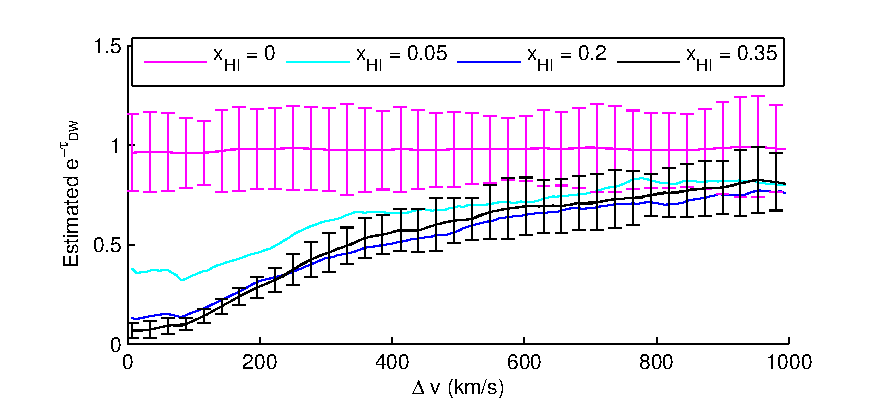
\includegraphics[width=8cm]{fig12a.eps}
  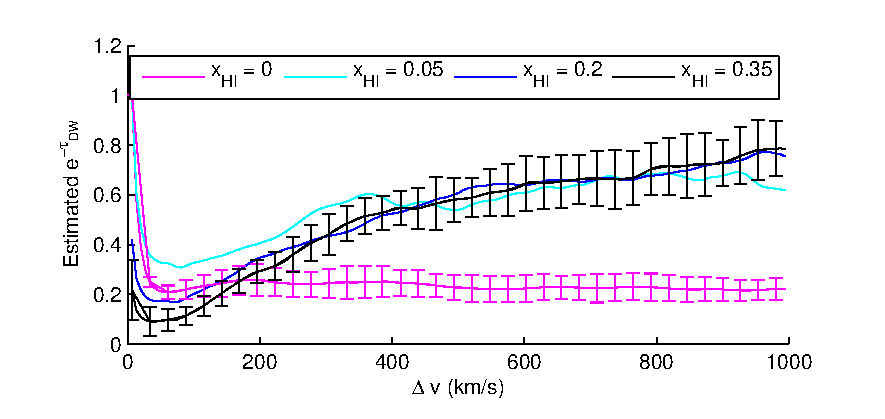
\includegraphics[width=8cm]{fig12b.eps}
  \caption{Using the \lyb\ forest to estimate damping-wing-less \lya\ transmission. The above figure shows the estimated \textit{shape} of stacked damping wing absorption for $\axhi = 0$ (magenta), 0.05 (cyan), 0.22 (blue), and 0.35 (black). The curves have been normalized to have their mean values peak at 1. Additionally, we show error bars for the fully ionized case and $\axhi = 0.35$ case which indicate the scatter in the curves between groups of 20 spectra. The left-hand plot is obtained by using a large ensemble of mock spectra to model a mapping between stacked \lyb\ transmission and stacked damping-wing-less \lya\ transmission and then applying this to groups of 20 spectra. Meanwhile, the right-hand figure plots the ratio of the stacked \lya\ flux to the stacked \lyb\ flux, providing a simplified estimate of the damping wing contribution to the absorption for each case. }
  \label{fig:DWShape}
\end{figure}


\section*{Appendix C: Extended damping wing Absorption from Correlated HI Islands} \label{sec:Correlation}


As mentioned in \S\ref{sec:Damping Wing Results}, and seen in \Fig{fig:LyaResults}, \ref{fig:LyaResults_LowF}, \& \ref{fig:HIRES_LyaResults_Noisy}, stacked \lya\ transmission outside of large saturated regions in a significantly neutral IGM displays excess absorption extending significantly past the scale of an isolated damping wing. To explain this, we seek to model the expected transmission outside of a neutral region, incorporating the correlation between the neutral region at the origin and neighboring neutral regions.  In order to simplify the calculation, while capturing the main effect, we ignore correlations between the neighbors themselves -- i.e., we only include the correlation between the neutral region at the origin and the neighbors and ignore inter-neighbor correlations.

Ignoring correlations between the neighboring neutral regions, we can approximate them as following a Poisson distribution and consider the total absorption contributed by these neutral islands or ``clouds'' following
\cite{Zuo}. Suppose that on average $m$ clouds contribute to the absorption at a given region of the spectrum.
Let $F_k \equiv e^{-\tau_1}e^{-\tau_2}\cdots e^{-\tau_k}$ denote the transmission when $k$ clouds reside along the line of sight and impact the given spectral region, with $\tau_i$ being the optical depth of the $i$th cloud. If we allow the clouds to be placed independently and if they have equal optical depths, then:
\begin{align}
\left\langle F_{k} \right\rangle &\equiv \left\langle e^{-\tau_1}e^{-\tau_2}\cdots e^{-\tau_k} \right\rangle = \left\langle e^{-\tau_1} \right\rangle \left\langle e^{-\tau_2} \right\rangle \cdots \left\langle e^{-\tau_k} \right\rangle = \left( e^{-\tau} \right)^{k}.
\end{align}
Using this expression, we can calculate the ensemble-averaged transmission by averaging over all the possible numbers of intervening clouds:
\begin{align}
\left\langle F \right\rangle &= \sum_{k = 0}^{\infty} \text{Pois}(k;m) \left\langle F_k \right\rangle = \sum_{k = 0}^{\infty} \dfrac{e^{-m}}{k!}m^{k}\left\langle e^{-\tau}\right\rangle^{k} = e^{-m}\sum_{k = 0}^{\infty} \dfrac{\left(me^{-\tau}\right)^{k}}{k!} \\
&= e^{-m}e^{me^{-\tau}} = e^{-m\left(1-e^{-\tau}\right)}.
\end{align}
Let us define the quantity $\tau_{\text{eff}}$ as
\begin{align}
e^{-m\left(1-e^{-\tau}\right)} &\equiv e^{-\tau_{\text{eff}}} \\
\tau_{\text{eff}} &\equiv m\left(1-e^{-\tau}\right).
\end{align}
We now have the absorption from neighboring clouds, characterized by the parameter $\tau_{\text{eff}•}$. 

We just need to adapt this slightly to the problem at hand. Suppose that  -- with certainty -- there is a neutral region located at $v=0$ and let us consider the excess absorption, above random, contributed
by neighboring neutral regions. 
First, the optical depth at $v = \Delta v$ that is contributed by a neighboring cloud located at $v = v'$ will depend on $|\Delta v - v'|$: clouds closer to $v = \Delta v$ will have larger optical depths at that corresponding frequency. We can account for this by substituting $\tau \to \tau(|\Delta v - v'|)$, according to \Eqn{eq:HIDW}.  Next, the expected number of HI islands in a region with velocity extent $\dd v'$ nearby our stacking location can be approximated as
\begin{align}
m &\approx \dd v' \left\langle n_{\text{HI}} \right\rangle (1 + \xi_{\text{HI,HI}}(v'))
\end{align}
where $\left\langle n_{\text{HI}} \right\rangle$ is the average number of HI islands per interval $\dd v'$ and $\xi_{\text{HI,HI}}(v')$ is the correlation function between the centers of neutral regions separated by $v'$. 
From here, we can model the effective optical depth at a given velocity separation due to neighboring HI islands, $\tau_{\text{eff}}(\Delta v)$, as
\begin{align}
\tau_{\text{eff}}(\Delta v) &= \int \dd v' \left\langle n_{\text{HI}} \right\rangle \left(1+\xi_{\text{HI,HI}}(v')\right) \left[ 1 - e^{-\tau(|\Delta v - v'|)} \right] \label{eq:taueff}.
\end{align}
In other words, the excess effective optical depth from neighboring systems involves the convolution of the absorption profile around each region with the correlation function of the neutral regions. 
This is analogous to the ``two-halo'' term in the halo model (e.g. \citealt{Cooray:2002dia}).

Thus, the model for the overall stacked transmission outside of neutral regions, also incorporating the damping wing from the central neutral region, becomes:
\begin{align}
\left\langle F \right\rangle (\Delta v) &= e^{-\tau_{\text{DW}}(\Delta v)}e^{-\tau_{\text{eff}}(\Delta v)}.
\end{align}
This model requires two inputs. First, it requires the correlation function between the centers of neutral regions, $\xi_{\text{HI,HI}}(v')$, which can be calculated from a model of the underlying ionization field. Second, the optical depth profile for neutral regions, $\tau (|\Delta v - v'|)$, is a function of the size of the neutral regions, per \Eqn{eq:HIDW}. While the neutral regions in the mock spectra take on a range of sizes, we make the simplifying approximation here -- but not in the body of this paper -- that the neutral regions at a given neutral fraction have one typical size and denote this $L_{\text{typical}}$ with a corresponding extent in velocity space $v_{\text{ext}}$. This effectively results in the optical depth profile of an individual neutral island in the right hand side of \Eqn{eq:taueff} being described by a piecewise function
\begin{align}
\tau_{\text{DW}}(\Delta v) = \begin{cases} \infty &\mbox{if } |\Delta v| < v_{\text{ext}}/2 \\ \dfrac{\tau_{\text{GP}}R_{\alpha}c}{\pi}\left[ \dfrac{1}{\Delta v - v_{\text{ext}}/2} - \dfrac{1}{\Delta v + v_{\text{ext}}/2} \right] &\mbox{otherwise.} \end{cases}
\end{align}
Next, we would like to compare this model against results using mock spectra. We do this by first generating mock spectra which \textit{only include absorption from neutral islands}, since this is the only type of absorption incorporated in our model, and stack these mock spectra at the HI/HII boundaries. To be clear, while the model curve described above adopted a fixed $L_{\text{neut}}$ for the purpose of calculating a $\tau_{\text{eff}}$, the mock spectra here are generated using the same simulated ionization fields as throughout the rest of the paper, with a wide range of sizes for the underlying neutral regions. 

To obtain a model for the stacked transmission, we first calculate the correlation function between the centers of neutral regions using the mock underlying ionization fields and also choose a value for $L_{\text{typical}}$ to be used in the optical depth profile. Additionally, in Eq. \ref{eq:taueff}, the $(1 + \xi_{\text{HI,HI}}(v'))$ term effectively breaks our integral into two pieces: the first representing the mean absorption from neutral regions and the second representing the excess or reduced absorption at $v = \Delta v$ due to the clustering of neutral islands. For our case, we are only concerned with the \textit{excess} absorption, so we make the replacement $(1 + \xi_{\text{HI,HI}}(v')) \to \xi_{\text{HI,HI}}(v')$.

Therefore, by providing a value for $L_{\text{typical}}$ and measuring $\xi_{\text{HI,HI}}(v')$, we can get a estimate for the mean transmission outside of neutral regions which incorporates absorption from spatially-correlated neighboring regions. In the left panel of \Fig{fig:HaloParts}, we plot an example of this for $\axhi = 0.22$. We show the modelled damping wing absorption from the central neutral region in blue, the modelled absorption from neighboring neutral islands and their damping wings in cyan, and the product of these in black. For comparison, we show the stacked transmission in the mock spectra in magenta, shifted by $v_{\text{ext}}/2$ to account for stacking occurring at HI/HII boundaries instead of at the center of neutral regions. All curves have been divided by the mean transmission. 
After taking $L_{\text{typical}} = 3.2 \mpch$, we find good agreement between the above model and the stacked transmission. The precise agreement should be taken with a grain of salt, since the model
makes several simplifying assumptions, especially that the neutral regions have a fixed size. However, the model does demonstrate that clustered neutral islands should lead to extended excess
absorption, significantly beyond the scale of an individual damping wing.

In the right panel of \Fig{fig:HaloParts}, we show the comparison between the stacked transmission (solid) and modelled transmission (dashed) for $\axhi = 0.35$ (black), 0.22 (blue), and 0.05 (cyan), where each curve has been multiplied by the mean transmission for clarity. In generating these plots, we have assumed $L_{\text{typical}} = 2.5 \mpch$, $3.2 \mpch$, and $0.75 \mpch$ for $\axhi = 0.35$, 0.22, and 0.05, respectively. We again find a very nice agreement between the modelled and stacked transmission, further confirming that spatially-correlated regions are indeed responsible for the significantly-extended excess absorption.

\begin{figure}[h]
  \centering
	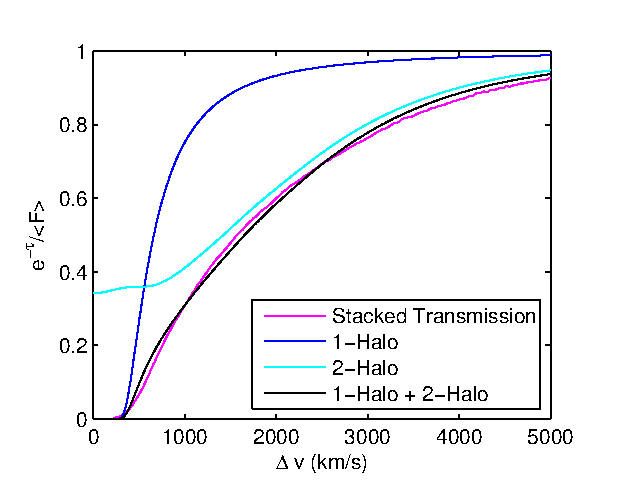
\includegraphics[width=8cm]{fig13a.eps}
	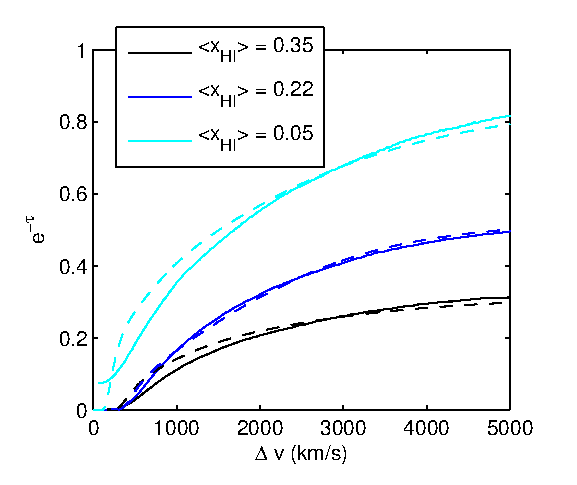
\includegraphics[width=8cm]{fig13b.eps}
  \caption{Model for the extended damping wing absorption. The left panel shows the components of our model for stacked transmission outside of a neutral region compared to the stacked transmission using mocked spectra (magenta) for $\axhi = 0.22$. We show the absorption due to the central neutral region (blue), average absorption due to neighboring, clustered neutral regions (cyan), and the product of the two transmissions (black). These are denoted in the legend as ``1-Halo'', ``2-Halo'', and ``1-Halo + 2-Halo'' in analogy with the halo model. In the right-hand panel, we show the comparison between the modelled transmission (dashed) and transmission from stacked mocked spectra (solid) for $\axhi = 0.35$ (black), 0.22 (blue), and 0.05 (cyan). The curves in the right-hand figure have been multiplied by the mean transmission (computed here ignoring resonant absorption for illustration).  In this appendix, the stacking is done at the HI/HII boundaries and only damping wing absorption is incorporated to demonstrate the extended excess absorption owing to correlated neighboring systems.}
  \label{fig:HaloParts}
\end{figure}



% the code below specifies where the figures are stored
\ifpdf
    \graphicspath{{igm_temperature/figures/PNG/}{bubble_finding/figures/PDF/}{bubble_finding/figures/}}
\else
    \graphicspath{{igm_temperature/figures/EPS/}{example_chapter/figures/}}
\fi


% ----------------------------------------------------------------------
%: ----------------------- content ----------------------- 
% ----------------------------------------------------------------------
\chapter{On Modelling and Measuring the Temperature of the $z \sim 5$ IGM}\label{sec:IGMTemperature}

\section{Introduction} \label{sec:IGMTemperatureIntro}

The temperature of the low density intergalactic medium (IGM) after reionization retains information about
when and how the gas was heated during the Epoch of Reionization (EoR) (e.g. \citealt{1994MNRAS.266..343M,Hui:1997dp,Theuns:2002yc,Hui:2003hn}).
The temperature of the IGM in turn
impacts the statistical properties of the Ly-$\alpha$ forest towards background quasars and so the absorption in the
forest provides ``fossil'' evidence regarding the timing and nature of reionization. Scrutinized carefully, this
fossil may therefore improve our understanding of reionization. For example, the IGM will likely be cooler at $z \sim 5$ if most of the IGM volume
reionized at relatively high redshift, near e.g. $z \sim 10$, than if reionization happened later, near say $z \sim 6$. If reionization occurs
early, the gas has longer to cool and reaches a lower temperature than if it happens late, at least provided the gas is heated to a fixed
temperature at reionization. In addition, the IGM temperature should be inhomogeneous, partly as a result of spatial
variations in the timing of reionization across the universe (\citealt{Trac:2008yz,Cen:2009bg,Furlanetto:2009kr}). Careful measurements of the IGM temperature after reionization should hence
constrain the average reionization history of the universe, and may potentially reveal spatial variations around the average 
history as well.

Two separate phases of reionization are likely relevant for understanding the thermal history of the IGM: an early period
of hydrogen reionization during which hydrogen is ionized, and helium is singly ionized by star-forming galaxies, and a later period 
in which helium is doubly-ionized by quasars, i.e. HeII reionization. Hydrogen reionization completed sometime 
before $z \sim 6$ or so (e.g. \citealt{Fan:2005es}, although it might conceivably end
as late as $z \sim 5$ -- see \citealt{McGreer:2011dm,Mesinger:2009mv,Lidz:2007mz}) ,
while mounting evidence suggests HeII reionization finished by $z \gtrsim 2.5-3$ (see e.g. \citealt{Worseck:2011qk,Syphers:2011uw} and references therein). 
Many of the existing IGM temperature measurements focus on redshifts of
$z \sim 2-4$ (\citealt{Schaye:1999vr,Ricotti:1999hx,McDonald:2000nn,Zaldarriaga:2000mz,Theuns:2001my,Lidz:2009ca});
in this case the temperature is likely strongly influenced by HeII
reionization (e.g. \citealt{McQuinn:2008am}) and so these measurements
mostly constrain helium reionization rather than hydrogen reionization.

In order to best constrain hydrogen reionization using the
thermal history of the IGM, temperature measurements
at higher redshift ($z \gtrsim 5$) are required. Indeed, recent work
has started to probe the temperature at these early times. In particular,
the recent study by \citet{Becker:2012aq} includes a measurement
at $z=4.8$; \citet{Bolton:2011ck} and \citet{Raskutti:2012qz} determine
the $z \sim 6$ temperature in the special ``proximity zone'' region of the Ly-$\alpha$
forest close to the quasar itself; and the analysis in \citet{Viel:2013fqw} starts to bound
the $z \gtrsim 5$ IGM temperature, although these authors focus on placing
limits on warm dark matter models.

The temperature at these higher redshifts is unlikely to be significantly impacted by HeII reionization. 
In addition, the ``memory'' of intergalactic gas to heating during the EoR gradually fades and so measurements as close as possible
to the EoR should, in principle, be most constraining.
It is not, however, obvious that the IGM temperature can be measured accurately enough 
from the $z \gtrsim 5$ Ly-$\alpha$ forest to exploit the sensitivity of the high redshift temperature to the properties of reionization. In particular, the forest is highly absorbed by $z \sim 5$ with $z \gtrsim 6$ spectra showing
essentially complete Gunn-Peterson (\citealt{1965ApJ...142.1633G}) absorption troughs (\citealt{Becker:2001ee,Fan:2005es}). An interesting question is then: what is the highest redshift at which it is feasible
to measure the IGM temperature from the Ly-$\alpha$ forest?

Towards this end, the goal of this chapter is to both model the thermal state of the $z \sim 5$ IGM, incorporating inhomogeneities in
the hydrogen reionization process, and to quantify the prospects for actually measuring the IGM temperature using $z \gtrsim 5$ Ly-$\alpha$ forest absorption spectra. The outline of this chapter is as follows. In \S \ref{sec:IGMTemperaturesims}, we describe
the numerical simulations used in our analysis. In \S \ref{sec:IGMTemperaturereion_hist}, we present plausible example models for
the reionization history of the universe and describe our approach for modeling inhomogeneous reionization. We adopt a semi-analytic approach
for modeling the resulting thermal history of the IGM, as described in \S \ref{sec:IGMTemperaturetherm_hist}. In this section, we also quantify
the statistical properties of the temperature field in several simulated reionization models.
 Finally, in \S \ref{sec:IGMTemperaturetemp_measure} we discuss how to measure
the temperature from the $z \sim 5$ Ly-$\alpha$ forest, and forecast how well it may be measured with existing data. Our main conclusions
are described in \S \ref{sec:IGMTemperatureconclusions}.

This work partly overlaps with previous work which also recognized the importance of, and modeled, temperature inhomogeneities in the $z \sim 5$ IGM
and considered some of the observable implications (\citealt{Trac:2008yz,Cen:2009bg,Furlanetto:2009kr}).\footnote{\citet{Lai:2005ha} also considered
temperature fluctuations from hydrogen reionization, but these authors focused on $z \sim 3$ where -- as they discussed -- these fluctuations should be small and swamped
by effects from HeII reionization.} One key difference with this earlier work is
that we consider a more direct approach for measuring the temperature of the $z \sim 5$ IGM from the Ly-$\alpha$ forest. Our modeling of
the thermal state of the IGM is closely related to that in \citet{Furlanetto:2009kr}, except that we implement a similar general approach
using numerical simulations, which allow us to construct mock Ly-$\alpha$ forest spectra and to measure the detailed statistical properties
of these spectra. The works of (\citealt{Trac:2008yz,Cen:2009bg}) use radiative transfer simulations to model hydrogen reionization and the
thermal history of the IGM and so these authors track
some of the underlying physics in more detail than we do here. However, our approach here is faster, simpler, and more flexible, while we believe
that it nevertheless captures many of the important processes involved. 


\section{Simulations}
\label{sec:IGMTemperaturesims}

Our analysis makes use of two different types of numerical simulations. First, we use the ``semi-numeric'' scheme of
\citet{Zahn:2006sg} to model reionization; this algorithm is performed 
on top of the dark matter simulation of \citet{McQuinn:2007dy}. The \citet{McQuinn:2007dy} simulation
tracks $1024^3$ dark matter particles in a simulation volume with a co-moving sidelength of $130$ Mpc/$h$. 
Using the semi-numeric technique allows
us to capture the impact of inhomogeneities in the reionization process, while providing the flexibility to explore a range
of possible reionization models. In these models, we assume that the gas distribution closely traces the simulated dark
matter distribution. We discuss the impact of this approximation when relevant.
As we will describe,
we map between the redshift of reionization of each gas element and its temperature at high redshift using the technique
of \citet{Hui:1997dp}; this mapping depends on the density of each gas element. We then produce mock Ly-$\alpha$ forest
spectra, according to the usual ``fluctuating Gunn-Peterson approximation'' (e.g. \citealt{MiraldaEscude:1995bu,Croft:2000hs}) although here 
we additionally account for the temperature
variations from inhomogeneous reionization.

We also make use of one of the smoothed particle hydrodynamic (SPH) simulations from \citet{Lidz:2009ca}. These simulations 
were run using the code Gadget-2 (\citealt{2005MNRAS.364.1105S}). This simulation tracks $2\times 1024^3$ particles
(with equal numbers of dark matter and baryonic particles) in a $50$ Mpc/$h$ simulation box. In these calculations, we ignore
the inhomogeneity of the reionization process. We use these simulations to more faithfully capture the gas distribution (for
gas elements that reionize at a given time). In constructing mock Ly-$\alpha$ forest spectra from these simulations, we first
modify the simulated gas temperatures, according to various prescriptions, in order to test how sensitive the statistical properties of the
absorption are to the gas temperature.


\section{Reionization Histories}
\label{sec:IGMTemperaturereion_hist}


In an effort to explore how the thermal state of the post-reionization 
IGM depends on the reionization history of the universe, we consider several example reionization histories. 
Our aim is to consider models that result in a wide range of possible thermal histories, while broadly maintaining 
consistency with current observational constraints on reionization. 

For simplicity, we assume (as is common) that early galaxy populations produce ionizing photons at a rate
that is directly proportional
to the rate at which matter collapses into halos above some minimum mass. The minimum mass describes the 
host halo mass above which galaxies form readily; here we adopt $M_{\rm min} = 10^9 M_\odot$. We compute the collapse fraction
from the Sheth-Tormen halo mass function (\citealt{Sheth:1999su}).
With these assumptions, the volume averaged ionization fraction ($\avg{x_i}$) obeys the following differential equation (\citealt{1987ApJ...321L.107S,1999ApJ...514..648M}):
\beqa
\frac{d\avg{x_i}}{dt} = \zeta \frac{df_{\rm coll}}{dt} - \frac{\avg{x_i}}{\bar{t}_{\rm rec}}.
\label{eq:xi_ode}
\eeqa
The first term on the right hand side of the equation describes the rate at which neutral atoms are ionized, while the second
term on the right hand side accounts for ionized atoms that recombine. The recombination time ($\bar{t}_{\rm rec}$) depends on the clumpiness of the IGM,
parametrized by a ``clumping factor'', $C=\avg{n_e^2}/\avg{n_e}^2$, and the temperature of the IGM. In solving this equation -- and for this purpose only -- we assume an isothermal
IGM. We approximate the clumping factor and the temperature as independent of redshift.
Adopting the case-B recombination rate in solving this equation, a temperature of $T_0 = 2 \times 10^4$ K, and $C=3$ (see e.g. \citealt{Pawlik:2008mr,McQuinn:2011aa} for a discussion regarding plausible values of the clumping factor) gives
\beqa
\bar{t}_{\rm rec} = 0.93 {\rm Gyr} \left[\frac{3}{C}\right] \left[\frac{1+z}{7}\right]^{-3} \left[\frac{T_0}{2 \times 10^4 K}\right]^{0.7}.
\label{eq:trec}
\eeqa
Solving the differential equation, Eq. \ref{eq:xi_ode}, suffices to compute the average ionization fraction as a function of redshift, given
the minimum mass and efficiency, $\zeta$, of the ionizing sources.

In order to 
model reionization inhomogeneities, we use the ``semi-numeric'' scheme of \citet{Zahn:2006sg}, which is based on the excursion set model of reionization developed
in \citet{Furlanetto:2004nh}.
This scheme captures the tendency for halos -- and hence galaxies -- to form first in
regions that are overdense on large scales, and to reionize before more typical locations in the universe. In the simplest version of the semi-numeric
scheme, recombinations are considered only in an average sense and are treated as simply reducing the overall efficiency at which atoms are ionized. Let us denote the resulting efficiency factor as $\tilde{\zeta}(z)$ to distinguish it from the above ionizing efficiency factor $\zeta$.
As we explain subsequently, we allow this efficiency factor to be redshift dependent. We can then consider the condition that
a region of co-moving size $R$ is ionized. In the initial conditions, the mass enclosed within this co-moving region is 
$M=4 \pi R^3 \avg{\rho_M}/3$, with $\avg{\rho_M}$ denoting the average matter density per co-moving volume. The condition for this
region to be ionized is then:
\beqa
\tilde{\zeta}(z) f_{\rm coll}(> M_{\rm min} | \delta_M, M) \geq 1.
\label{eq:ion_cond}
\eeqa
In this equation $f_{\rm coll}(> M_{\rm min} | \delta_M, M)$ is the conditional collapse fraction, i.e., the fraction of mass in halos
above the minimum mass ($M_{\rm min}$) in a region of linear overdensity $\delta_M$. Here $\delta_M$ denotes the overdensity when the
linear density field is smoothed on mass scale $M$. 

In order to tabulate a reionization redshift for many grid cells across the volume
of our simulation, we smooth the density field -- linearly evolved from the initial conditions -- on a range of mass scales, starting from large scales and stepping downward until
we reach the scale of each simulation cell. For each simulation cell, and across all smoothing scales considered, we record
the highest redshift at which the ionization barrier (Eq. \ref{eq:ion_cond}) is crossed. This highest crossing redshift is considered
to be the reionization redshift, $z_r$, for the cell in question. We tabulate reionization redshifts for each 
of $512^3$ grid cells. This provides us with a reasonable model for the expected spatial variations in the redshift of 
reionization -- and the coherence scale of these inhomogeneities -- across the simulation volume. 

Note that here we approximate the excursion set model as determining the redshift at which each {\em volume element} is reionized, although
in reality mass elements move from their initial positions, and overdense regions expand less rapidly than typical locations. This approximation
is commonly made, and is reasonable given the large size of the ionized regions (\citealt{Furlanetto:2004nh}) and the correspondingly large coherence scale of
the spatial variations in the reionization redshift.

Another ingredient we use from the \citet{McQuinn:2007dy} simulation is the evolved non-linear
dark matter density field, interpolated onto the same grid (using CIC interpolation) as the reionization redshifts. For our calculations with this simulation, we generally assume that
the gas distribution follows the simulated, gridded dark matter distribution. Note that the smoothing introduced by gridding the dark matter particles is
comparable to the Jeans smoothing scale:
the co-moving Jeans wavenumber for isothermal gas
at $10^4$ K, is $k_J = 13 h$ Mpc$^{-1}$ at $z=5$ which is comparable to the Nyquist wavenumber of the grid, $k_{\rm Nyq} = 12 h$ Mpc$^{-1}$.
More relevant, however, is the ``filtering scale'' -- essentially a time-averaged Jeans scale -- and this should be smaller than the Jeans scale by around a factor of a few (\citealt{Gnedin:1997td}). In any case a single global smoothing only roughly approximates the full effect of Jeans smoothing. We will return to discuss this further in \S \ref{sec:IGMTemperaturetemp_measure} and \S \ref{sec:IGMTemperaturewave_inhomog}. In particular, in order to approximately 
capture the impact of small scale structure and thermal broadening in our mock quasar spectra, we will add small-scale structure using a lognormal model. Although using the gridded dark matter density field to represent the gas distribution is inadequate for making detailed mock spectra, it suffices for our model of the temperature distribution of the low density gas.

Returning to further consider the semi-numeric modeling, an important caveat is that this algorithm does not return precisely the
expected volume-averaged ionization fraction (see the Appendix of \citealt{Zahn:2006sg} for a discussion). 
Here we simply tune $\tilde{\zeta}(z)$
to produce the desired redshift evolution of the ionization fraction. 
Although this procedure is not
ideal, small adjustments to the ionizing efficiency factor have little impact on 
the size of the ionized regions at a given volume-averaged ionization fraction, $\avg{x_i}$,
and so this approach is adequate for our present purposes.


\begin{figure}
\bc
\includegraphics[width=9cm]{f1.eps}
\caption{Example reionization histories. The red triangles show the simulated volume-average ionization fraction in our semi-numeric High-z reionization model, the
black squares are for the Mid-z reionization scenario, and the blue pentagons are for a low redshift (Low-z) reionization model. The black dashed line shows the reionization
history computed by solving Eq. \ref{eq:xi_ode} with $\zeta=46$, $M_{\rm min} = 10^9 M_\odot$ and $C=3$. The semi-numeric
efficiency parameters $\tilde{\zeta}(z)$ in the Mid-z case have been tuned to match this model.}
\label{fig:xi_examp}
\ec
\end{figure}

The redshift evolution of the volume-averaged ionization fractions are shown in Fig. \ref{fig:xi_examp} for three example models. The symbols
show the average ionized fraction from the simulation cube at different redshifts. We call the three examples in the
figure the ``Low-z'' model, the ``Mid-z'' model, and the ``High-z'' model. The Mid-z model adopts a redshift dependent efficiency factor
of the form $\tilde{\zeta}(z) = 35 (1+z/13)^{1.75}$ for $z \leq 12$ and $\tilde{\zeta}=35$ for $z > 12$.
For comparison, the black dashed line shows
the solution to Eq. \ref{eq:xi_ode} for a model with $\zeta=46$, $C=3$, and $M_{\rm min} = 10^9 M_\odot$. Hence the semi-numeric scheme
in the Mid-z model has been tuned to return the ionized fraction expected from Eq. \ref{eq:xi_ode} for a plausible model.
The Low-z and High-z models are similar to the Mid-z model, except that
the efficiency factor in the semi-numeric models has been adjusted to $\tilde{\zeta}(z)=12 (1+z/11)^{0.60}$ at $z \leq 10$ and to
$\tilde{\zeta}(z)=12$ at $z > 10$ for the Low-z model and to a constant efficiency factor $\tilde{\zeta}(z)=70$ for the High-z model. (Although these 
alternative models were not themselves explicitly tuned to match particular solutions to Eq. \ref{eq:xi_ode}, the general
behavior is similar to in the Mid-z model except that reionization happens a little later/earlier in the Low-z/High-z model and
so these models also appear reasonable).

It is also useful to quantify the timing and duration of reionization, as well as the optical depth to Thomson scattering ($\tau_e$), in each model. 
Defining the ``completion'' of reionization as the redshift where the volume averaged ionization fraction first reaches $\avg{x_i} =1$,
the High-z model completes at $z=9.6$,
the Mid-z model at $z=6.7$, and the Low-z model at $z=5.8$. As one measure of the ``duration'' of reionization, we consider the redshift spread over which $\avg{x_i}$ evolves from
$\avg{x_i}=0.1$ to $\avg{x_i} = 1$. This duration is $\Delta z = 2.7, 4.3, 3.5$ for the High-z, Mid-z, and Low-z models. Note that the duration
is the longest in the Mid-z model because the ionizing efficiency factor $\tilde{\zeta}(z)$ has the strongest redshift dependence in this case. 
The electron scattering optical depths are $\tau_e = 0.088, 0.066, 0.052$ for the High-z, Mid-z, and Low-z reionization
models respectively. These values assume that the fraction of helium that is singly ionized is identical to the fraction of hydrogen that
is ionized, and ignore the slight boost expected from the free
electrons produced after HeII reionization, which we do not track in this work. 

The present constraint on $\tau_e$ from Planck CMB temperature anisotropy data (\citealt{Ade:2013zuv}), combined with the E-mode polarization power spectrum
at large angular scales from WMAP nine year data (\citealt{Bennett:2012zja}), is $\tau_e = 0.089^{+0.012}_{-0.014}$. Most of the constraining power here
comes from the WMAP polarization data. Hence our High-z model produces a $\tau_e$ close to the presently preferred value, the Mid-z model is low by $1.6-\sigma$, while the Low-z model is too low by $2.6-\sigma$. Hence our lower redshift reionization models are already marginally
disfavored, but they are still certainly worthy of further investigation. The Planck collaboration should soon announce new large-scale CMB
polarization measurements; the improved frequency coverage of the Planck satellite should help guard against foreground contamination, and
further test these models for $\tau_e$.
Although the current $\tau_e$ constraints allow higher reionization redshift models than the three
examples considered here, the $z \sim 5$ IGM temperature is insensitive to the reionization redshift
if reionization happens above $z \gtrsim 10$ (\S \ref{sec:IGMTemperaturetherm_hist}, \citealt{Hui:2003hn}). While viable, we need not consider such models 
explicitly here since in these cases the $z \sim 5$ temperature will be similar to that in our High-z model.


\section{The Thermal State of the IGM}
\label{sec:IGMTemperaturetherm_hist}

We now explore how the thermal state of the $z \sim 4-6$ IGM depends on the reionization history of the Universe, using
the example histories of the previous section. In this section, we focus mostly
on the Low-z and High-z models since they span a fairly wide range of possibilities for the IGM temperature at the redshifts
of interest.

The key equation describing the thermal evolution of a gas element in the IGM is (e.g. \citealt{Hui:1997dp}): 
\begin{align}
\frac{dT}{dt} =& -2 H T + \frac{2 T}{3 (1+\delta)}\frac{d\delta}{dt} + \frac{T}{\mu}\frac{d\mu}{dt} \nonumber \\
& + \frac{2 \mu m_p}{3 \rho k_B}\left({\mathcal H} - \Lambda\right).
\label{eq:tev}
\end{align}
 The first term on the right hand side accounts for adiabatic cooling owing to the overall expansion of the universe. The second 
term describes
adiabatic heating/cooling from structure formation, i.e. from gas elements contracting/expanding. In the third and fourth terms, $\mu$ is the mean mass per free particle in the gas, in units of the proton mass. The third term accounts for the temperature
change that occurs because the mean mass per particle may change with time. ${\mathcal H}$ describes the 
heating term, while $\Lambda$ is the cooling function of the gas. These terms describe the heat gain and loss per unit volume, per unit
time, in the gas. 

Let us first summarize the qualitative behavior of the solutions to Eq. \ref{eq:tev}, focusing on the low density intergalactic gas that fills most of the volume of the universe (see also \citealt{1994MNRAS.266..343M,Hui:1997dp,Hui:2003hn,Furlanetto:2009kr}). During reionization, most gas elements are rapidly ionized and change their ionization
fraction by order unity.\footnote{Sufficiently overdense regions/clumps may be only gradually ionized as reionization proceeds and the ionizing 
radiation field incident upon them grows in intensity, 
but we will neglect these, assuming that partly neutral clumps fill only a small fraction of the volume within mostly ionized regions.}
The excess energy of the ionizing photons (above the ionization threshold) goes into the
kinetic energy of the outgoing electrons, which quickly share their energy with the surrounding gas, and
raise its temperature. The first thing to consider is hence the initial temperature reached at reionization.
Provided the gas becomes highly ionized, its temperature boost during reionization
depends only on the {\em shape} of the spectrum -- and not the amplitude -- of the radiation that ionized
it. 

In detail, we expect gas elements to be ionized by radiation with a range of spectral shapes. This should be the case both
because the intrinsic ionizing spectrum will vary from galaxy to galaxy, and because
the spectral shape may be hardened by intervening absorption, which will itself vary spatially depending on the column density
of neutral gas between an ionizing source and an absorber. On the other hand, the ionized regions during hydrogen reionization
likely grow under the collective influence of numerous (yet individually faint) dwarf galaxies (e.g. \citealt{Robertson:2013bq}), and so
some of these variations may average down, provided gas elements are ionized by a combination of several sources and
the ionizing radiation arrives along various different pathways.
In any case, modeling the precise temperature input during reionization and its spatial variations requires full radiative
transfer simulations and is well beyond the scope of our approach here.
We adopt this uniform temperature boost approximation throughout, and discuss plausible values for the input temperature subsequently. Note also that in this case
the temperature boost during reionization is 
independent of density: extra heat is put into the overdense regions since more
atoms are ionized in these regions, but the heat is shared across the larger number of particles in the overdense parcel.

After a gas element is reionized, it settles into ionization equilibrium and the
UV radiation from the ionizing sources keeps the gas highly ionized (at least for the low density gas parcels that fill most
of the volume of the IGM). 
In ionization equilibrium, each recombination is balanced by a photoionization and the ionizations in turn heat
the gas; the average time between recombinations in the low density IGM is long, and so the heat input from photoionization
is significantly reduced after a parcel becomes highly ionized during reionization. In 
addition, the spectral shape of the ionizing radiation incident on
a typical gas element should soften -- i.e., the average heat input per photoionization should drop -- after reionization as the optical depth to ionizing photons decreases (\citealt{Abel:1999vj}).\footnote{In reality, the spectral
softening depends on how progressed reionization is {\em globally} since the hardening from absorption depends on the 
density and ionization
state of all of the gas between a source and an absorber. Here we neglect this by fixing the spectral shape incident on each
gas element after it is ionized.}

The dominant cooling processes are adiabatic cooling from the expansion of low density gas parcels and 
Compton cooling off of the CMB. As a result of cooling, although gas elements that reionize at the same time start off with identical temperatures,
irrespective of their density, parcels with differing densities will not stay at the same temperature.
In particular, the
low density elements expand and cool faster than typical regions, while overdense regions recombine faster and thus -- in ionization equilibrium -- gain 
more heat from
photoionizations after reionization. In addition, sufficiently overdense regions will be heated by adiabatic contraction.
\citet{Hui:1997dp} showed that this competition between adiabatic cooling/heating, Compton cooling, and photoionization heating,
drives the intergalactic gas to generally land on a tight temperature-density relation of the form
$T=T_0 (1 + \delta)^{\gamma-1}$. Both the temperature at mean density, $T_0$, and the slope of the temperature density relation, $\gamma$,
depend on the reionization redshift; $T_0$ falls off and $\gamma$ becomes steeper as the gas cools after reionization, until the gas
gradually loses memory of the heating during reionization. In the 
previous work of \citet{Hui:1997dp}, however, all of the gas was assumed to reionize
at the same redshift. Here we would like to generalize this to incorporate spatial variations in the redshift of
reionization (see also \citealt{Furlanetto:2009kr} and \citealt{Hui:2003hn}).

\subsection{Modeling the Thermal State}
\label{sec:IGMTemperaturetemp_mod}

In general, to follow the thermal evolution in Eq. \ref{eq:tev} we should combine this equation with equations specifying the
evolution of the ionized fraction of each different particle species. However, for our present application a simpler approach should suffice.
In particular, we start by assuming that each parcel is heated to a common temperature, $T_r$, at its reionization redshift, $z_r$. We then 
follow the subsequent
thermal evolution after a gas element is ionized by assuming ionization equilibrium and that each element is highly ionized (as in \citealt{Furlanetto:2009kr}). More specifically,
we assume that both HI and HeI are highly ionized, but that HeII is not yet ionized, i.e., that HeII reionization starts
later than the high redshifts of interest
for our study. We further assume the gas is composed of only hydrogen and helium, neglecting metal line cooling, and also molecular hydrogen cooling,
which should be very good approximations for the low density IGM. In addition to adiabatic heating/cooling and Compton cooling, 
we track HI photoheating, HeI photoheating, and recombination cooling of HII/HeII using the rate expressions in the Appendix
of \citet{Hui:1997dp}. We ignore collisional ionizations, and HI/HeI/HeII line excitation cooling: neglecting these processes should
be a good approximation for the low density and highly ionized gas that fills most of the IGM volume after reionization. Furthermore, we ignore other potential heating sources such as shock heating, galactic winds, blazar heating, etc..(see e.g. \citealt{Hui:2003hn,Chang:2011bf} and references
therein for a discussion). In the Appendix
we also derive approximate solutions using linear perturbation theory (incorporating only HI photoheating, Compton cooling, and
adiabatic cooling/heating), that are useful for fast and fairly accurate estimates (see also \citealt{Hui:1997dp}).

In principle we could calculate the adiabatic expansion/contraction term (second term in Eq. \ref{eq:tev}) directly from the \citet{McQuinn:2007dy} 
simulation, at least
under the approximation that the gas distribution traces the simulated dark matter density field. Here we instead follow the approach of
\citet{Hui:1997dp} and compute this term for tracer elements assuming their density evolution obeys the Zel'dovich approximation (\citealt{1970A&A.....5...84Z}).
As mentioned earlier, we do, however, extend this calculation to consider gas elements with a range of different reionization redshifts. 

The basic premise here is that gas elements with identical reionization redshifts should land on a well-defined temperature-density
relation (as supported by the tests in \citealt{Hui:1997dp} and subsequent work); we can determine this relation by solving Eq. \ref{eq:tev} for many sample gas parcels.
Incorporating, however, the spread in reionization redshifts, and that the reionization redshift of each parcel may
correlate with its density, a perfect temperature-density relation will {\em not} generally be a good description. In other words,
we follow sample gas parcels to determine the mapping between the temperature-density relation at a given redshift and
the reionization redshift and temperature, i.e., this is used to determine $T_0(z|z_r,T_r)$ and $\gamma(z|z_r, T_r)$. These
mappings can then be applied to our reionization simulation to determine the temperature of any gas element, given its
reionization redshift and overdensity. To determine $T_0(z|z_r,T_r)$ and $\gamma(z|z_r,T_r)$, we follow the thermal evolution for $20,000$ tracer elements
for many different
reionization redshifts, assuming their density evolves according to the Zel'dovich approximation, and fit separate power-laws
for each $z, z_r$, and $T_r$. 

In the Zel'dovich approximation, the density field evolves according to the equation:
\beqa
1 + \delta = \frac{1}{\rm{det}[\delta_{ij} + D(t) \psi_{ij}]},
\label{eq:zeldo}
\eeqa
with $\psi_{ij}$ denoting the initial deformation tensor, and $D(t)$ denoting the linear growth factor (normalized to unity today). The density evolution of a tracer element can then be specified by the eigenvalues of the local initial deformation 
tensor.  
As in \citet{Hui:1997dp} and \citet{1995ApJ...449..476R}, we can construct realizations of the density evolution in the Zel'dovich approximation 
by randomly drawing eigenvalues of $\psi_{ij}$ from the expected probability distribution (\citealt{1970Afz.....6..581D}). We do this following \citet{Hui:1999ku,Bertschinger:1993zv}. 


In our fiducial model, we take the temperature at reionization to be $T_r = 2 \times 10^4$ K (see \citealt{Furlanetto:2009kr,McQuinn:2012bq} for a discussion
of this choice). In calculating the photoionization heating term after a gas parcel reionizes, we assume that the specific
intensity of the ionizing radiation 
is a power-law in frequency close to the hydrogen photoionization threshold, $J(\nu) \propto \nu^{-\alpha}$ with $\alpha=1.5$.
As mentioned previously, the heat input is insensitive to the amplitude of the ionizing radiation, provided the gas is highly ionized. This spectral shape is intended
to be somewhat harder than expected for the {\em intrinsic spectrum} of the ionizing sources, since intervening absorption will harden
this spectrum (\citealt{1993ApJ...418...28Z,Hui:2003hn,Furlanetto:2009kr}).


\subsection{Simulated Temperature Field}
\label{sec:IGMTemptemp_sim}

\begin{figure}
\bc
\includegraphics[width=9cm]{f2.eps}
\caption{Thermal state of gas elements with a given reionization redshift, as a function of that redshift. In each case, the gas elements are heated to
a temperature of $T_r=2 \times 10^4$ K during reionization, and the residual photo-heating after reionization is computed assuming that the
(hardened) spectral index of the ionizing sources is $\alpha=1.5$ near the HI photoionization edge. {\em Top panel:} The temperature
at mean density ($T_0$) for gas elements at each of $z=4.5,5.0$ and $5.5$ as a function of their reionization redshift. {\em Bottom panel:} This is similar to the top panel, except it shows the slope of the temperature-density relation ($\gamma-1$) rather than $T_0$. Note that although we assume that gas
elements with a given reionization redshift all land on a well defined temperature-density relation, this will not generally be
a good description once we account for the spread in reionization redshift across the universe. }
\label{fig:tden_v_zr}
\ec
\end{figure}

We now examine the properties of the simulated temperature field, modeled as described in the previous section. 
First, we consider the mapping between the temperature at mean density, $T_0$, and the slope of the temperature-density
relation, $\gamma$, for gas at various redshifts, given the reionization redshift, $z_r$, of each gas element. This
is shown, for our baseline set of assumptions, in Fig. \ref{fig:tden_v_zr} for each of $z=4.5,5.0,$ and $z=5.5$.
The values of $T_0$ are close to the temperature at reionization ($T_r = 2 \times 10^4$ K) for gas elements that ionized at redshifts
just above $z=5.5$, since these elements have had very little time to cool. On the other hand, gas parcels with higher $z_r$ have had longer to cool
and are hence at lower temperatures. For instance, gas elements that reionized at $z_r = 8$ have cooled down to $T_0 = 8,800$ K by
$z = 5.5$, more than a factor of two below the temperature at reionization. The temperatures of gas elements that reionize at sufficiently
high redshift, however, become insensitive to the precise redshift of reionization. In particular, gas elements that
reionize above $z_r \gtrsim 10$ are all at $T_0 = 6,700$ K at $z=5.5$, irrespective of $z_r$. This results mainly
because Compton cooling is very efficient at high redshift ($z \gtrsim 10$), and effectively erases the 
memory of the photoheating during
reionization (\citealt{Hui:1997dp}). Indeed, this is the main reason that we don't consider still higher redshift reionization
models, although they would be allowed by the present $\tau_e$ constraints as discussed in \S \ref{sec:IGMTemperaturereion_hist} (but perhaps disfavored by other data sets, see e.g. \citealt{Robertson:2013bq,Kuhlen:2012vy} for recent summaries.): 
the thermal state of the IGM is insensitive to higher redshift reionization models.

The bottom panel is similar to the top panel
except here we plot $\gamma-1$ versus $z_r$. Gas elements that reionize just above $z = 5.5$ are close to isothermal, while
elements that ionize at $z_r \gtrsim 10$ have a steeper slope, $\gamma = 1.53$. The $T_0$ and $\gamma-1$ curves at $z=4.5$ and $z=5.0$ illustrate
less sensitivity to $z_r$, since gas elements at these redshifts have had longer to cool down from their initial
temperatures at reionization. Nevertheless, the models at these lower redshifts still certainly do show some 
dependence on $z_r$. 

\begin{figure}[t]
\bc
\includegraphics[width=7cm]{f3a.ps}
\includegraphics[width=7cm]{f3b.ps}
\caption{Reionization redshifts and temperatures at $z=5.5$ in the low-z reionization model.
{\em Left panel:} The reionization redshifts for a narrow slice ($0.25$ Mpc/$h$ thick) through
the simulation. Each slice is $130$ Mpc/$h$ on a side. The red regions indicate locations with the highest reionization redshifts across
the simulation slice, while the dark regions are the last to be reionized. {\em Right panel:}
The temperature of the same slice as in the top panel. The red areas in this panel show the
hottest locations in the slice, and correspond to the dark regions in the top panel that
are reionized late. The dark blue regions in the temperature slice, on the other hand, are the coolest regions that reionized
first. The color scales are chosen so that $99\%$ of simulation cells in the slice shown here have redshifts and temperatures falling 
between the minimum and maximum values on the color bar.}
\label{fig:tslice_lowz}
\ec
\end{figure}

We then use the curves plotted in Fig. \ref{fig:tden_v_zr} as a mapping to predict the temperature of various grid cells in our
simulation given their overdensities, $\delta$, and reionization redshifts, $z_r$. This procedure allows us to model the temperature
field across the entire simulation volume at various redshifts. 

\begin{figure}[t]
\bc
\includegraphics[width=7cm]{f4a.ps}
\includegraphics[width=7cm]{f4b.ps}
\caption{Reionization redshifts and temperatures at $z=5.5$ in the high-z reionization model. Identical to Fig. \ref{fig:tslice_lowz},
except this figure shows the contrasting High-z model. Note that the color scale in this case also encompasses $99\%$ of the reionization
redshifts and temperatures in the simulation slice, but that these ranges are different than in the previous figure.}
\label{fig:tslice_highz}
\ec
\end{figure}

Figs. \ref{fig:tslice_lowz} and \ref{fig:tslice_highz} show the result of applying the mapping (at $z=5.5$) to the simulated density field.\footnote{In practice, we apply the mapping to the simulated density field at slightly higher redshift ($z=6.9$) since we don't currently
have outputs from this simulation at the lower redshifts of interest. Using the higher redshift output artificially reduces the variance in the density field, and the
resulting structure in the temperature field somewhat. For our present purposes, this is not important. The main effect of boosting the density
variance should be to increase the minimum and maximum density contrasts shown in scatter plots such as Fig. \ref{fig:tden_lowz}. 
Importantly, this has little impact on the median temperature-density relation and the scatter around this relation for the range of
density contrasts in our scatter plots. We have tested this explicitly using a lognormal approximation to the density field at $z=4.5$ and
$z=5.5$.} Specifically, these figures show thin slices ($0.25$ Mpc/$h$ thick) through the simulation volume, with the top
panel showing the reionization redshift and the bottom panel the corresponding temperature of cells in
the simulation volume. In the Low-z model (Fig. \ref{fig:tslice_lowz}), the temperature field
has sizable spatial variations on large scales. As anticipated earlier, these result because of the spread in the timing of reionization
across the universe. As one can infer from the slice, the regions that are at low-density (when the density field
is smoothed on large-scales) -- i.e., the ``voids'' in the density distribution -- are the last to reionize. These
regions are at the highest temperature shortly after reionization because they have
had the least amount of time to cool (see also \citealt{Trac:2008yz,Furlanetto:2009kr}).

In contrast, the temperature field in the High-z model (Fig. \ref{fig:tslice_highz}) has mostly lost memory of
the heating during reionization and so the temperature variations are more subtle here. This is expected from Figs.
\ref{fig:xi_examp} and \ref{fig:tden_v_zr}: much of the gas in this model is reionized at $z_r \gtrsim 10$,
and efficient Compton cooling mostly removes the memory of reionization in this case.
The temperature variations that are apparent in the High-z model instead reflect the usual
temperature-density relation, as the competition between cooling and heating after reionization drives overdense
regions to larger temperatures. These temperature variations 
are primarily coherent on the Jeans/filtering scale and so, as evident from the simulation slices, these fluctuations are concentrated mostly
on smaller scales than the ones induced by the spread in the timing of reionization. 

\begin{figure}
\bc
\includegraphics[width=9cm]{f5.eps}
\caption{Temperature density relations at $z = 4.5$ and $z=5.5$ in the Low-z reionization model. The
blue points show the temperature and density of gas elements from the simulation at $z=5.5$, while
the black points are the same at $z=4.5$. The red short dashed line shows the median simulated temperature
as a function of density at $z=5.5$. The green long dashed line is the same at $z=4.5$.}
\label{fig:tden_lowz}
\ec
\end{figure}

\begin{figure}
\bc
\includegraphics[width=9cm]{f6.eps}
\caption{Temperature density relations at $z = 4.5$ and $z=5.5$ in the High-z reionization model.
Identical to Fig. \ref{fig:tden_lowz}, except the results here are for the High-z reionization model.}
\label{fig:tden_hiz}
\ec
\end{figure}

A further, more quantitative description is provided by constructing 
scatter plots of the temperatures of many simulated gas elements
as a function of their densities. This is shown in Figs. \ref{fig:tden_lowz} and \ref{fig:tden_hiz} for the Low-z and
High-z reionization models, respectively. Broadly similar results may be found in earlier work by \citet{Trac:2008yz} and \citet{Furlanetto:2009kr}. The red short-dashed line in each figure shows the median gas temperature at $z=5.5$, while
the green long-dashed line is the median temperature at $z=4.5$. Fig. \ref{fig:tden_lowz}
shows that the temperature of the $z=5.5$ IGM is generally rather high -- and has a large amount of scatter at low
densities -- in the Low-z reionization model. By contrast, the temperature
in the High-z reionization model (Fig. \ref{fig:tden_hiz}) is smaller -- e.g., by 60\% for the median temperature near
the cosmic mean density  -- as is the scatter. In the Low-z model the median temperature is a fairly flat function of density
for gas less dense than the cosmic mean. 

Note that although the regions that have low density -- when the density field is averaged on large scales -- ionize last and are mostly
hotter than denser regions (see Fig. \ref{fig:tslice_lowz}), this does not fully ``invert'' the temperature-density relation. This is because the density field on the scale of the simulation grid (and at the Jeans scale) is
only somewhat correlated with the larger scale density variations that determine the spread in the timing of reionization
in our model. In any case, in agreement with previous work (\citealt{Trac:2008yz,Furlanetto:2009kr}), the usual temperature-density
relation is a poor description of the thermal state of the IGM in the Low-z model at $z=5.5$. 
At slightly lower redshifts, $z=4.5$, the temperature
has dropped somewhat and the scatter in the Low-z model has partially subsided, although it is still substantial. The median
temperatures in the two reionization models are closer to each other by $z=4.5$, but they still differ by 30\%. 

\begin{figure}
\bc
\includegraphics[width=9cm]{f7.eps}
\caption{Power spectrum of temperature fluctuations in various models. The curves show the power spectrum of 
$\delta_{T_0}(\x) = (T_0(\x) - \avg{T_0})/\avg{T_0}$ from the simulated models. The blue dotted line, the black solid line, and the red short-dashed line
are the power spectra at $z=5.5$ in the Low-z, Mid-z, and High-z models respectively. The black long-dashed line
shows the $\delta_{T_0}$ power spectrum at $z=4.5$ in the Mid-z model to illustrate how the temperature fluctuations fade with
time.}
\label{fig:power_tzero}
\ec
\end{figure}

It is also useful to calculate the power spectrum of temperature fluctuations in each model. Since we are assigning
a value of $T_0$ and $\gamma$ to each grid cell in the simulation volume, we can easily consider the power 
spectrum of $T_0$ rather
than the power spectrum of the full temperature field. The advantage of considering the power spectrum of $T_0$ is that this power
spectrum
vanishes in the case of homogeneous reionization. In the case of homogeneous reionization, the 
temperature is a power-law in the gas density, and so the full temperature field still has (mostly small scale)
fluctuations sourced directly by density inhomogeneities. Hence we consider here the power spectrum of $T_0(\x)$, or more
precisely the power spectrum of $\delta_{T_0}(\x) = (T_0(\x) - \avg{T_0})/\avg{T_0}$. Although the power spectrum of this field
is not directly observable, it nevertheless helps to characterize the temperature fluctuations from reionization.
 
The power spectra in some of our models are shown in Fig. \ref{fig:power_tzero}.
Specifically,
the curves show $\Delta^2_{T_0} = k^3 P_{T_0}(k)/(2 \pi^2)$, the contribution to the variance of $\delta_{T_0}$ per natural logarithmic
interval in $k$, i.e., per ${\rm dln}(k)$.
In the Low-z model,
the temperature fluctuations peak at a level of around $\sqrt{\Delta^2_{T_0}(k)} \approx 15\%$. 
We should keep in mind, however, that the scatter in the temperature at lower density is larger than
at mean density (see Fig. \ref{fig:tden_lowz}). As a result, the power spectra of $T_0$ shown here hence do not fully
capture the impact of inhomogeneous reionization, but they do nevertheless illustrate the spatial scale of the reionization induced
inhomogeneities as well as their redshift and model dependence.
The power spectra ($\Delta^2_{T_0}$)
are evidently fairly flat functions of $k$. This is not surprising, since the power spectra of the fluctuations in the ionization field
are also rather flat functions of $k$ during most of the EoR (e.g. \citealt{McQuinn:2006et}). At the same redshift, the $\delta_{T_0}$ power spectrum in
the Mid-z Model is $\approx 3$ times smaller in amplitude than in the Low-z model, while the amplitude of variations ($\Delta^2_{T_0}(k)$) in the High-z model are $\approx 300$ times smaller than in the Low-z model. As discussed previously, the
small fluctuations in the High-z model result because Compton cooling is efficient at high redshift and this rapid cooling effectively erases the memory of
heating at higher redshifts. Comparing the black solid and dashed lines illustrate how the fluctuations fade from $z=5.5$ to $z=4.5$ in the Mid-z model.

These models illustrate the dependence of the thermal history of the IGM on the timing of reionization; let us briefly summarize
our main findings here.
The IGM temperature for models in which
a significant fraction of the IGM volume is reionized at relatively low redshift, near $z \sim 6$, is correspondingly larger than if most of the gas is reionized
at higher redshift. In addition, the late reionization models produce sizable temperature inhomogeneities with 
fluctuations on scales as large
as $\sim$ tens of co-moving Mpc. 

\subsection{Variations around Fiducial Parameters}
\label{sec:IGMTemperaturetat_reion}

Before we proceed to discuss the observable signatures of the IGM temperature models, it is interesting to consider
how variations around our fiducial assumptions regarding the reionization temperature, $T_r$, and the shape
of the ionizing spectrum after reionization might impact the resulting thermal state of the IGM. To investigate this,
we consider models where the reionization temperature is $T_r = 3 \times 10^4$ K and $T_r=1 \times 10^4$ K to
contrast with our fiducial model in which $T_r = 2 \times 10^4$ K. The low $T_r$ model requires sources with
extremely soft ionizing spectra, and is meant to represent a lower limit to the plausible reionization temperature,
while the higher temperature $T_r = 3 \times 10^4$ K case is more reasonable (e.g. \citealt{McQuinn:2012bq}).  
In addition, for our fiducial reionization temperature
we produce models with (post reionization) spectral shapes of $\alpha=0.5$ and $\alpha=2.5$ to compare with our baseline assumption of
$\alpha=1.5$.

\begin{figure}[t]
\bc
\includegraphics[width=9cm]{f8.eps}
\caption{Thermal state at $z=5.5$ for various reionization temperature and spectral shape models. This is similar to the
$z=5.5$ curves in Fig. \ref{fig:tden_v_zr}, except here we vary the reionization temperature, $T_r$, and the spectral shape,
$\alpha$. Increasing $T_r$ leads to a higher $T_0$ and a flatter $\gamma$ for recently reionized gas parcels, while parcels
that reionize at sufficiently high redshifts are insensitive to $T_r$. A harder ionizing spectrum after reionization 
(smaller $\alpha$) leads mostly to a slightly larger value of the asymptotic temperature achieved at high $z_r$.
The harder spectrum also slightly hastens the transition of $\gamma$ to its asymptotic value.}
\label{fig:temp_v_treion}
\ec
\end{figure}

First, we consider how our models for $T_0(z=5.5|z_r)$ and $\gamma(z=5.5|z_r)$ depend on the reionization temperature
and spectral shape, i.e., we regenerate the models of Fig. \ref{fig:tden_v_zr} for different values of $T_r$ and $\alpha$.
The results of these calculations are shown in Fig. \ref{fig:temp_v_treion}. The first feature to note is that $T_0$ and
$\gamma$ are independent of $z_r$ and $T_r$ in the limit of large reionization redshift: efficient cooling wipes out the memory
of the early heating history. On the other hand, the $z=5.5$ temperature is naturally quite sensitive to the reionization temperature
if reionization occurred relatively recently. One consequence of this is that the {\em scatter} in the $z \sim 5$ temperature
will be larger in low redshift reionization models for cases with larger reionization temperatures: a high reionization temperature
increases the temperature contrast between recently reionized gas parcels and those that reionized early. The increased scatter in
these models may potentially boost the observability of the temperature inhomogeneities induced by spatial variations in the timing
of reionization, as we explore subsequently.  

Another important point is that increasing $T_r$ in a high reionization redshift model will not help to mimic the $z \sim 5$ temperature
in a lower redshift reionization model, since the gas that reionized at high redshift reaches an asymptotic temperature that is insensitive
to $T_r$. On the other hand, decreasing $T_r$ (as in the $T_r = 10^4$ K curves) in a low reionization redshift model will certainly diminish the distinction between
this model and higher reionization redshift models. As we will see, however, the larger scatter and flatter trend of temperature with density
in the low $z_r$, low $T_r$ model offer potential handles for distinguishing between these models and higher reionization redshift scenarios.

Next we consider how the results vary with changes in the spectral shape, $\alpha$, as shown in the figure. These variations have a relatively minor effect. Adopting
a harder ionizing spectrum (smaller $\alpha$) after reionization increases the amount of residual late-time photoheating. This 
thereby raises
the asymptotic temperature and the asymptotic value is reached earlier. Quantitatively, the asymptotic temperature is $20\%$
higher in the $\alpha=0.5$ case than in our fiducial $\alpha=1.5$ model, and $18\%$ smaller for $\alpha=2.5$. The dependence on $\alpha$
is relatively mild compared to other uncertainties in our modeling and so we don't consider it further here.

\begin{figure}
\bc
\includegraphics[width=9cm]{f9.eps}
\caption{Temperature density relation at $z=5.5$ for various reionization temperatures in the High-z and Low-z models. The ``X''s in the 
legend indicate the color of the points in the corresponding models, while the dashed lines in the same models have different colors to
promote visibility. The models in the legend are listed from top to bottom: the highest points and line (indicating the median temperature
at various densities) show the $T_r = 2 \times 10^4$ K, Low-z model; next is the $T_r = 1 \times 10^4$ K, Low-z model;
then the $T_r = 3 \times 10^4$ K, High-z model; and finally the $T_r = 3 \times 10^4$ K, High-z model.
}
\label{fig:tden_v_treion}
\ec
\end{figure}

Another perspective is to construct scatter plots in the temperature-density plane and plot median temperature-density relations for various models, as in Fig. \ref{fig:tden_lowz} and Fig. \ref{fig:tden_hiz}. This is shown for gas at $z=5.5$ in Fig. \ref{fig:tden_v_treion}. Consider first the two High-z models (the bottom two sets of points and dashed lines in the figure), which show the results of assuming $T_r = 2 \times 10^4$ K (bottom-most case with red points and a black dashed line), and $T_r = 3 \times 10^4$ K (shown as blue points and a cyan line, just above the bottom-most model). This shows that the results in this model are insensitive to $T_r$: this is as anticipated from
Fig. \ref{fig:temp_v_treion}. The next model is a Low-z case and has $T_r = 1 \times 10^4$ K (green points and blue line). This
model is clearly closer to the High-z reionization model than our fiducial Low-z case, which is shown in the figure as the upper most
black points with red line fit. However, the median temperature at low density and the scatter in the temperature 
are both larger in the Low-z, low reionization
temperature model than in the High-z models. If the scatter in the temperature, and the trend of temperature with density can be measured
observationally, this may help break the partial degeneracies between reionization redshift and temperature. 




\section{Measuring the Temperature of the $z \sim 5$ IGM}
\label{sec:IGMTemperaturetemp_measure}

We now turn to consider the impact of the thermal state of the IGM on the properties of the $z \sim 5$ Ly-$\alpha$ 
forest, and
on the possibility of extracting these signatures to learn about reionization. The effects of temperature
on the statistics of the Ly-$\alpha$ forest are discussed, for example, in \citet{Lidz:2009ca}. The three main effects 
are: higher temperatures produce more Doppler broadening; the recombination rate of the absorbing gas is temperature
dependent with hotter gas recombining more slowly, leading to less neutral gas and less absorption; hotter gas leads
to more Jeans smoothing, with the precise impact of this smoothing depending on the entire prior thermal history of the absorbing gas
(\citealt{Gnedin:1997td}). 

The enhanced Doppler broadening and Jeans smoothing in models with high temperatures each act to reduce the amount of small-scale structure in the Ly-$\alpha$ forest.
These two effects are not, however, entirely degenerate: Jeans smoothing filters the gas distribution in three dimensions, while
Doppler broadening smooths the optical depth field along the line of sight 
(e.g. \citealt{Zaldarriaga:2000mz}). Previous studies suggest that Doppler broadening impacts the small scale structure in the
forest more than Jeans smoothing, at least near $z \sim 3$ (\citealt{Zaldarriaga:2000mz,Peeples:2009ue,Lidz:2009ca}). At $z \sim 5$, we 
expect Jeans smoothing to have more impact, however: the high opacity in the Ly-$\alpha$ line at these redshifts implies that even slight
density enhancements can give rise to noticeable absorption lines, and these slight density variations may be erased by Jeans
smoothing. Unfortunately, it is challenging to model the impact of Jeans smoothing while incorporating a realistic model
for inhomogeneous reionization and photoheating. This requires hydrodynamic models that resolve the filtering scale, while capturing
a large enough volume to model patchy reionization. Furthermore, the filtering scale depends on the entire prior thermal history. 
In this chapter, we defer this challenge to future work and assume that the effect of Jeans smoothing is sub-dominant
to that of Doppler broadening. We caution that Jeans smoothing might, however, enhance the impact of patchy reionization and 
modeling it may be necessary to robustly interpret future measurements. 

In any case, the small-scale structure in the Ly-$\alpha$
forest should be sensitive to the thermal state and the thermal history of the IGM, and so we now consider an approach for estimating the
amplitude of small-scale structure in the forest.
Here we will use the basic technique described in \citet{Lidz:2009ca}, except applied here to simulated data at higher redshift
where there is more absorption in the forest. The first issue we aim to explore here is to what extent the temperature of
the IGM is measurable at higher redshift, where the forest is significantly more absorbed. A second goal is to explore the
impact of the temperature inhomogeneities modeled in the previous section.

We briefly outline the approach of \citet{Lidz:2009ca} for measuring the small-scale structure -- and thereby extracting constraints on the 
IGM temperature -- here for completeness.
In this approach, each spectrum is convolved with a Morlet wavelet filter and
the smoothing scale of this filter is tuned to extract the amplitude of the small scale power spectrum in the forest as a function of
position across each spectrum. The Morlet filter is a plane wave, multiplied by a Gaussian and in configuration space
may be written as:
\beqa
\Psi_n(x) = K \rm{exp}(i k_0 x) \rm{exp}\left[-\frac{x^2}{2 s_n^2}\right].
\label{eq:filt_real}
\eeqa
The Fourier space counterpart, when the normalization constant $K$ is fixed so the filter has unit power (see \citealt{Lidz:2009ca}) is:
\beqa
\Psi_n(k) = \pi^{-1/4} \sqrt{\frac{2 \pi s_n}{\Delta u}} \rm{exp}\left[-\frac{(k - k_0)^2 s_n^2}{2}\right].
\label{eq:filt_four}
\eeqa
In the above equation, $\Delta u$ is the size of each spectral pixel in velocity units and $s_n$ is a suitable smoothing scale (also in velocity units) chosen
to extract the small scale power, and we set $k_0 s_n = 6$ (see \citealt{Lidz:2009ca}). Each mock spectrum is convolved with the above filter. We work with the transmission
fluctuation field, $\delta_F(x) = (F(x) - \avg{F})/\avg{F}$ where $F=e^{-\tau}$ is the transmission and $\avg{F}$ is the
ensemble-averaged mean transmitted flux. 

The transmission fluctuation, convolved with the wavelet filter, is:
\beqa
a_n(x) = \int dx^\prime \Psi_n(x - x^\prime) \delta_F(x^\prime),
\label{eq:field_filt}
\eeqa
The amplitude of this filtered field, at position ``$x$'' is given by
\beqa
A(x) = |a_n(x)|^2,
\label{eq:waveamp}
\eeqa
and characterizes the amount of small-scale structure in the transmission field. 
We generally smooth this field with a top-hat of length $L$,
\beqa
A_L(x) = \frac{1}{L} \int_{-\infty}^{\infty} dx^\prime \Theta(|x - x^\prime|; L/2) A(x^\prime),
\label{eq:smoothed_waveamp}
\eeqa
where $\Theta$ is a top-hat function. The quantity $A_L(x)$ is a measure of the average small scale power across
different portions of a quasar spectrum, and should broadly trace the temperature of corresponding regions in the IGM,
with cold regions giving a larger $A_L$ than hot regions. 


\subsection{Hydrodynamic Simulations: Perfect Temperate-Density Relation Models}

As a first test, we take high redshift outputs from the hydrodynamic simulation (see \S \ref{sec:IGMTemperaturesims}) and impose temperature-density relations
before producing mock quasar spectra. This test ignores the impact of inhomogeneous reionization, but it nonetheless provides
some intuition for how well our approach can constrain the IGM temperature.

\begin{figure}
\bc
\includegraphics[width=9cm]{f10.eps}
\caption{Example sightlines and wavelet amplitudes for two different models of the IGM temperature at $z \sim 5$.
The top panel shows $\delta_F(x)$ for an example sightlines with $T_0 = 2.5 \times 10^4$ K, $\gamma=1.3$ (red dashed) and the same sightline except with $T_0 = 7.5 \times
10^3$ K, $\gamma=1.3$ (black solid). The bottom panel shows the smoothed wavelet amplitudes, $A_L$, along each spectrum.
The lower temperature model has more small scale structure and larger wavelet amplitudes. The smoothing scale $s_n=51$ km/s here, while
$\Delta u = 3.2$ km/s and $L=1,000$ km/s.}
\label{fig:examp_sightlines}
\ec
\end{figure}

Fig. \ref{fig:examp_sightlines} shows an example sightline, $50$ Mpc/$h$ in length, extracted from the hydrodynamic simulation at $z=5$
for each of two different temperature-density relation models. The top panel shows the transmission fluctuation, $\delta_F$, for
models with $\gamma=1.3$ and each of $T_0 = 7.5 \times 10^3$ K and $T_0 = 2.5 \times 10^4$ K while the bottom panel shows the
smoothed wavelet amplitudes, $A_L$, in each model. In this case, the smoothing scale $s_n$ is set to $s_n=51$ km/s, the pixel
size to $\Delta u = 3.2$ km/s, and $L=1,000$ km/s. 
In each case the intensity of the ionizing background has been renormalized
so that the global mean transmitted flux is $\avg{F}=0.20$. This is the mean transmitted flux implied by extrapolating 
the recent best-fit measurement of \citet{Becker:2012aq} to $z=5$.\footnote{Specifically, we use these authors' smooth functional fit to their measured effective optical
depth. This is an (approximate) fit to measurements in bins centered on redshifts from $z=2.15$ to $z=4.85$, and so our extrapolation of
this fit out to $z=5$ is only very slight.}

Although the differences between $\delta_F$ along the
two example sightlines are generally small, there are some noticeable differences. 
In particular, it appears that the ``spikes'' of
transmission in the colder model are more prominent. This is mostly a result of the larger Doppler widths in the hot model. 
At this redshift, the heights of the transmission spikes are often influenced
by nearby gas elements that are centered on
saturated or highly absorbed parts of the spectrum; the broad Doppler wings from this gas extend into 
adjoining unsaturated regions and thereby reduce the
height of neighboring transmission spikes. The spikes are
less impacted by the narrower Doppler wings in the colder model and remain more prominent.
Essentially, the forest has become
``inverted'' at these redshifts in comparison to at lower redshift. At sufficiently low redshift, the forest is mostly transmitted
with some prominent absorption lines interspersed. In the low redshift case most of the information about the IGM temperature comes from
narrow absorption lines. At high redshift, the forest is mostly absorbed and most of the information about the IGM temperature
is instead in the transmission spikes. 

In either case, the amount of small scale power in the Ly-$\alpha$ forest is indicative
of the temperature of the gas in the IGM. This is illustrated by the bottom panel of Fig. \ref{fig:examp_sightlines} for
the high redshift case considered here. This panel
shows the smoothed wavelet amplitudes along each line of sight. The smoothed wavelet amplitudes are larger in the cold IGM model,
with the largest differences occurring near $\Delta v \sim 4500$ km/s, close to several prominent transmission spikes in the models.

One possible complication is that long completely saturated regions will -- regardless of temperature -- have low wavelet amplitudes, $A_L$, since there
is no small scale structure in such regions. These saturated zones may in fact be {\em more prominent} in models with
low temperature since cold regions recombine more quickly, and hence have larger neutral fractions and suffer more absorption 
than hot regions.\footnote{Although the precise impact of the temperature on the wavelet amplitude PDFs shown here is not this transparent since we are comparing models at fixed
mean transmitted flux.} Fig. \ref{fig:examp_sightlines} suggests, however, that this is not a big effect at $z=5$, $\avg{F}=0.2$, although the saturated regions will be more prominent at higher redshift (see \S \ref{sec:IGMTemperaturewave_inhomog}). We can
guard against ``contamination'' from saturated regions by masking them before measuring the probability distribution
of the wavelet amplitudes, and by varying the smoothing scale $L$.


\begin{figure}
\bc
\includegraphics[width=9cm]{f11.eps}
\caption{Probability distribution of $A_L$ for various $T_0$ models at $z \sim 5$. Each model here assumes a perfect temperature
density relation with $\gamma=1.3$, and in each case the mean transmitted flux
has been fixed -- by adjusting the intensity of the ionizing background -- to $\avg{F_\alpha}=0.20$. As in Fig. \ref{fig:examp_sightlines}, 
the smoothing scale has been set to $s_n=51$ km/s, while
$\Delta u = 3.2$ km/s and $L=1,000$ km/s.}
\label{fig:pdf_amp}
\ec
\end{figure}

To characterize the variations of the wavelet amplitudes with temperature more quantitatively, we calculate the probability distribution function (PDF) of wavelet amplitudes for ensembles
of mock spectra generated from different temperature-density relation models. The results of these calculations are shown
in Fig. \ref{fig:pdf_amp}.
The PDF is quite sensitive to the temperature
at mean density in these models. For example, the location of the peak in the wavelet amplitude PDF is at an $A_L$ that is roughly
three times larger in the coldest model shown (with $T_0 = 7.5 \times 10^3$ K), compared to the hottest model considered here
($T_0 = 2.5 \times 10^4$ K). 
For the mean transmitted flux ($\avg{F}=0.20$) and $z=5$, the wavelet PDF for $s_n=51$ km/s is
sensitive mostly to densities near the cosmic mean. As a result, we find that the wavelet PDFs here depend strongly on
$T_0$, but are insensitive to $\gamma$, the slope of the temperature-density relation. It is hence important to keep in mind that our approach
for measuring the IGM temperature is only sensitive to the temperature of the IGM close to the mean density, and it is therefore not possible
to extract
the full trend of temperature with density shown in our models (e.g., Fig. \ref{fig:tden_lowz}).

Although the PDFs depend sensitively
on $T_0$, it is also clear that the wavelet amplitudes are not {\em perfect} indicators of the temperature. In the limit
that the temperature at mean density were the only quantity that determined $A_L$, these PDFs should approach delta functions
in $A_L$.
That the wavelet PDFs have some breadth is not, however, surprising: the temperature is clearly not the only quantity that
determines the small-scale structure in the forest. That said, Fig. \ref{fig:pdf_amp} looks promising and helps to motivate
further study.


\subsection{Degeneracy with the Mean Transmitted Flux}
\label{sec:IGMTemperaturedegen_amf}

One other potential issue, however, is that the wavelet PDF is also sensitive to the somewhat uncertain value of the mean transmitted 
flux, $\avg{F}$. Although the present statistical uncertainties on this quantity are $\sigma_{\avg{F}}/\avg{F} \leq 10\%$ near $z \sim 5$ (\citealt{Becker:2012aq}), the systematic uncertainties are significantly larger. In particular, it is difficult
to estimate the unabsorbed quasar continuum level, especially at the redshifts of interest for this study, where the
absorption in the forest is very large (e.g. \citealt{2008ApJ...681..831F}). The {\em measurement} of the wavelet PDF itself should, however,
be fairly robust to uncertainties in the level of the unabsorbed quasar continuum. This is the case because we consider the statistics
of the transmission fluctuations, $\delta_F = (F - \avg{F})/\avg{F}$, for which a (multiplicative) error in the continuum normalization
divides out (see \citet{Lidz:2009ca} for a discussion and tests with lower redshift data).


\begin{figure}[t]
\includegraphics[width=7cm]{f12a.eps}
\includegraphics[width=7cm]{f12b.eps}
\caption{Degeneracy with $\avg{F}$. {\it Left panel:} Although the PDF of $A_L$ is sensitive
to $T_0$, this effect is degenerate with the impact of varying $\avg{F}$. For instance, the model with $T_0 = 1.5 \times 10^4$ K
and $\avg{F} = 0.20$ is closely mimicked by a colder model with $T_0=7.5 \times 10^3$ K, yet a larger mean transmission of
$\avg{F} = 0.30$. {\it Right panel:} This illustrates that the degeneracy can be broken by measuring the (relatively) large
scale flux power spectrum. The curves here show the flux power spectrum, evaluated at a single convenient (larger-scale) wavenumber of $k=0.003$ s/km, 
in each $T_0$ model as a function of $\avg{F}$. The triangle and pentagon show the flux power for each model at the
$\avg{F}$ for which the wavelet amplitude PDFs are degenerate in the two models. The large scale flux power in these
two models differs appreciably and can be used to break the degeneracy. The red dotted and black dotted horizontal lines are intended 
only to guide the eye.}
\label{fig:degen_break}
\end{figure}


Nevertheless, we still need to know the mean transmitted flux very accurately: we use this measurement to in turn fix the 
intensity of the ionizing background at the redshifts of interest, which is itself quite uncertain. The amount of small
scale structure in the forest, and hence the model wavelet amplitudes, do depend on the overall mean transmitted flux. As a result,
while we should be able to measure the wavelet PDF without knowing the precise continuum normalization, our interpretation
of this measurement still requires knowing the mean transmitted flux.
To illustrate
this, we plot (in the top panel of Fig. \ref{fig:degen_break}) the $z=5$ wavelet amplitude PDF in a model with $T_0 = 1.5 \times 10^4$ K
and the preferred mean transmitted flux at this redshift ($\avg{F}=0.20$, red short-dashed line). As in Fig.  \ref{fig:pdf_amp},
the wavelet amplitudes are smaller in this model than in, for example, the cooler model with $T_0 = 7.5 \times 10^3$ K at the {\em same value of the} mean transmitted flux (blue long-dashed line in the top panel of Fig. \ref{fig:degen_break}). However, if we allow
the mean transmitted flux to increase in the colder model, the resulting wavelet PDF becomes similar to that in the hotter model. 
In particular, the black solid line shows a colder model with the mean transmitted flux increased to $\avg{F}=0.30$; this
closely matches the wavelet PDF in the hotter model at the smaller mean transmitted flux ($\avg{F}=0.20$). This particular value 
of the mean transmitted
flux, $\avg{F}=0.30$, is well outside the presently allowed range, given 
the statistical errors on current measurements. Nevertheless, the wavelet PDF clearly shows
some degeneracy between variations in $T_0$ and in $\avg{F}$. This invites further attention, especially given the systematic
concerns associated with estimating the unabsorbed continuum level.

One way to help break this degeneracy is to combine the measured wavelet PDF with a measurement of
the flux power spectrum on {\em larger scales}. This quantity is especially sensitive to the
mean transmitted flux, and the power spectrum of $\delta_F$ has the virtue -- like the wavelet PDF --
that it is insensitive to the overall normalization of the quasar continuum. On the other hand, on sufficiently large
scales,  the gentle fluctuations in the underlying quasar continuum still likely contaminate this measurement. However, there
should still be a useful range of scales where the structure in the forest dominates over that in the continuum (see e.g. \citealt{McDonald:2004eu}) and it is
these scales that we will consider to help break the $T_0-\avg{F}$ degeneracy.
 
To illustrate how the flux power measurement may help break this degeneracy, we plot the
amplitude of transmission fluctuations, $\Delta^2_F =k P_F(k)/\pi$, for a single example wavenumber ($k=0.003$ s/km in velocity units, or $k=0.39 h$ Mpc$^{-1}$
in co-moving units at $z=5$) as a function of mean transmitted flux.  The 1-D flux power spectrum ($P_F(k)$) is fairly flat on large scales and so the precise $k$ considered
here is not especially important.  The bottom panel of Fig. \ref{fig:degen_break} shows the flux power spectrum at $k=0.003$ s/km
as a function of $\avg{F}$ for the two values of $T_0$. In each case, $\Delta^2_F$ is a strong function of $\avg{F}$. The red
triangle and black pentagon show the power spectra in the $T_0 = 1.5 \times 10^4$ K and the $T_0 = 7.5 \times 10^3$ K
models respectively, for the values of the mean transmitted flux ($\avg{F}=0.20$ and $\avg{F}=0.30$) at which their wavelet
PDFs are degenerate. The large scale flux power spectra in these two models differ by the sizable factor of $1.7$. It should be
straightforward to measure the flux power spectrum on these scales to this level of accuracy, and so this measurement can help
pin down $\avg{F}$ and break the degeneracy.

One possible concern with this approach is that the precise relationship between $\Delta^2_F$ and $\avg{F}$ may be somewhat model dependent, and our inability to perfectly model the forest -- especially at high redshifts, potentially close to the EoR -- 
might lead us to draw spurious conclusions. At present, the only way to guard against this possibility is to test the goodness-of-fit
of our models for as wide a range of empirical tests as possible. Ideally, one would compare models with measurements of the
flux power across a wide range of scales (although significantly larger scales will be subject to contamination from power in
the quasar continuum), the wavelet PDF, the mean transmitted
flux, and perhaps the statistics of the Ly-$\beta$ forest as well (e.g. \citealt{Dijkstra:2003pd,Furlanetto:2009kr}).  


\subsection{Wavelet Amplitude PDFs in Inhomogeneous Reionization Models}
\label{sec:IGMTemperaturewave_inhomog}

With the results of the previous section as a guide, we now turn to consider the wavelet amplitude PDFs in the more realistic inhomogeneous temperature models developed 
in \S \ref{sec:IGMTemperaturetherm_hist}. In this case, we are using the dark matter simulations of \citet{McQuinn:2007dy} along with our model temperature
distributions.
Although the large volume of these simulations allows us to capture the reionization-induced inhomogeneities, they 
are not -- taken as is -- adequate
for capturing the small-scale structure in the Ly-$\alpha$ forest, which is the basic observable we aim to explore here. 

In order to make headway, we add small-scale structure to sightlines extracted from the simulation cube using the log-normal model, as in
\citet{2007ApJ...657...15K}. Briefly, we generate one-dimensional Gaussian random fields $\delta_G$ using the one-dimensional linear density power spectrum 
(scaled to the redshift of interest, and calculated after smoothing the three-dimensional linear power spectrum with a filter of the form $e^{-2 k^2/k_f^2}$ and $k_f = 30 h$ Mpc$^{-1}$ to loosely mimic the effect
of Jeans smoothing, \citealt{Gnedin:1997td}). From the Gaussian random realizations, we produce lognormal fields at high resolution using the transformation
$1 + \delta_{\rm LN} = e^{\delta_G - \sigma_G^2/2}$, where $\sigma_G^2$ is the variance of the Gaussian random field. As in \citet{2007ApJ...657...15K}
the lognormal field is modulated by the larger scale modes captured in the simulation ($\delta_{\rm sim}$) according to $1 + \delta = (1 + \delta_{\rm sim}) (1 + \delta_{\rm LN})$ with the (subscript-free) symbol $\delta$ denoting the density contrast with added small-scale structure. Similarly, using the simulated temperature in a coarse pixel (described by $T_0$ and $\gamma$), the temperature in 
a fine pixel becomes $T = T_0 (1+ \delta)^{\gamma-1}$.

The main disadvantage here is that the resulting sightlines have too much large scale structure: the lognormal field adds both large and small
scale modes to the simulation, and the simulation was not deficient in large scale power to begin with. This is partly mitigated by our using
a slightly higher redshift simulation output ($z=6.9$) than the redshift of interest. 
This simple approach is hence
imperfect, but the added small scale structure does nevertheless allow us to reliably model the impact of
thermal broadening on the resulting mock Ly-$\alpha$ forest spectra. As a test, we measure the flux power spectrum from the mock ``lognormal-enhanced'' sightlines and compare them with the flux power spectrum from mock spectra generated from the hydrodynamic simulation. The flux power spectrum from the
lognormal spectra is roughly $50\%$ larger than from the hydrodyamic simulations. However, the overall shape of the flux power is fairly well
captured in the lognormal case, and importantly, the shape of the flux power spectrum varies in a similar way in both calculations as
the temperature and thermal broadening are varied. Hence we believe that this approach suffices to capture the main impact of patchy reionization on
the small scale structure in the Ly-$\alpha$ forest. We caution, however, that a detailed comparison with upcoming measurements will certainly require
improvements here.

\begin{figure}
\bc
\includegraphics[width=9cm]{f13.eps}
\caption{Example sightlines and wavelet amplitudes from the Low-z and High-z reionization models. In the models here, the global mean flux
is $\avg{F}=0.1$ and $z=5.5$. In each panel the red dotted
line shows a sightline through the $T_r=3 \times 10^4$ K, Low-z reionization model while the black solid line is the same sightline,
except in this case the temperature field is drawn from the
High-z reionization model (with $T_r = 2 \times 10^4$ K). The simulated density and temperature fields have small scale structure
added according to the lognormal model, as described in the text. {\it Top panel:} The simulated temperature field. {\it Middle panel:}
The transmission field, $\delta_F$. {\it Bottom panel}: The smoothed wavelet amplitude with $L=1,000$ km/s, $s_n=34$ km/s, and
$\Delta u=2.1$ km/s. The transmission fluctuations and wavelet amplitudes are larger than in Fig. \ref{fig:examp_sightlines}, mostly because
of the lower mean transmitted flux adopted here.}
\label{fig:examp_wave}
\ec
\end{figure}


With this cautionary remark, we turn to consider the properties of mock spectra drawn from our inhomogeneous temperature models.
Fig. \ref{fig:examp_wave} shows typical example sightlines from the High-z and Low-z reionization models at $z=5.5$ and $\avg{F}=0.1$. The trends
are broadly similar to those 
in Fig. \ref{fig:examp_sightlines}: the colder models have more small scale structure than the hotter models. As a result, the transmission
field has more prominent spikes in the colder High-z model, and the smoothed wavelet amplitudes in this model (bottom panel) are 
larger than in the Low-z model. 
The inhomogeneous
models incorporate, however, the reionization-induced temperature variations that are not included in the previous model, although the impact of
these variations are generally hard to discern by eye. One can however identify that the prominent cold region in the middle of this sightline,
for example, corresponds to a pronounced peak in the smoothed wavelet amplitude field in each model. Note that the wavelet amplitudes and $\delta_F$
fluctuations are larger here than in Fig. \ref{fig:examp_sightlines} because here we consider $z=5.5$ and $\avg{F}=0.1$, while in the previous figure
we considered $z=5.0$ and $\avg{F}=0.2$. In addition, the lower transmitted flux considered here leads to more completely absorbed
regions in the mock Ly-$\alpha$ forest, and these regions have correspondingly low wavelet amplitudes. As discussed earlier, these regions do not
contain information about the IGM temperature. 


\begin{figure}
\bc
\includegraphics[width=7cm]{f14a.eps}
\includegraphics[width=7cm]{f14b.eps}
\caption{Probability distribution of $A_L$ for various reionization and temperature models at $z=5.5$. {\it Left panel:} In this panel all models are normalized
to $\avg{F}=0.2$. The solid black curve shows the wavelet amplitudes for the High-z reionization model (with $T_r = 2 \times 10^4$ K), while the red dotted and blue dashed curves show
Low-z reionization models with reionization temperatures of $T_r = 2 \times 10^4$ K and $T_r = 3 \times 10^4$ K respectively. The magenta dot-dashed line
shows a {\em homogeneous} temperature model for comparison. In this case, the temperature was set to match the median temperature in the
 Low-z, $T_r = 3 \times 10^4$ K model for
gas at the cosmic mean density; the broader distribution in the Low-z model reflects the impact of inhomogeneous reionization. 
{\it Right panel:} Identical to the top panel, but here the models fix $\avg{F}=0.1$. In each case, the filter scale and pixel size are set to $s_n=34$ km/s and $\Delta u=2.1$ km/s respectively,
while $L=1,000$ km/s.}
\label{fig:pdf_al_inhomog}
\ec
\end{figure}


More quantitatively, the resulting wavelet amplitude PDFs for some example inhomogeneous temperature models are shown in Fig. \ref{fig:pdf_al_inhomog}. Since the 
mean transmitted flux at this redshift ($z=5.5$) is somewhat uncertain, we compare models normalized to each of $\avg{F}=0.2$ (top panel) and $\avg{F}=0.1$ (bottom panel) in order
to illustrate the impact of varying $\avg{F}$. Extrapolating the best fit measurement from (\citealt{Becker:2012aq}), we find
$\avg{F}=0.13$ at $z=5.5$ so this range should approximately bracket the expected value, although the lower end of this range
is preferred. Note that there is some evidence that the mean transmitted flux decreases more rapidly above $z \sim 5.5$ or so compared to the evolution
expected from lower redshifts (e.g. \citealt{Fan:2005es}), and so this would
further favor the lower value, and perhaps even slightly smaller numbers than considered here. Nevertheless, it is worth considering the mean transmitted
flux dependence explicitly: even if $\avg{F}=0.2$ is reached at $z=5$ rather than $z=5.5$, the temperature fluctuations could be as large at $z=5$ as in our
$z=5.5$ models if reionization is more extended than considered here. 

In each case, the wavelet filter's smoothing scales are set to $s_n = 34$ km/s and $L=1,000$ km/s, while
the pixel size is $\Delta u = 2.1$ km/s.\footnote{The pixel size here matches that of typical Keck HIRES spectral pixels. Note that the smoothing scale, $s_n$, and pixel size, $\Delta u$, here are similar, but slightly different than used
in the previous section. The large scale smoothing, $L$, is identical.} In each panel, the PDF in the High-z model is compared to Low-z models for
two different reionization temperatures, $T_r = 2 \times 10^4$ K and $T_r = 3 \times 10^4$ K. In addition, we plot the wavelet amplitude PDF for a model
with a completely homogeneous temperature field. In this isothermal case the temperature is set to $T_0 = 1.44 \times 10^4$ K, matching the median
temperature near the cosmic mean density in the Low-z, $T_r = 3 \times 10^4$ K model. Homogeneous reionization 
models with the same $T_0$ but differing
$\gamma$ would give very similar results, since the wavelet amplitudes 
are sensitive to absorbing gas near the cosmic mean density for these values of the mean transmitted flux.
Comparing the $T_0 = 1.44 \times 10^4$ K isothermal model with the Low-z, $T_r = 3 \times 10^4$ K case helps to illustrate the impact of temperature
inhomogeneities.

First, we consider how the location of the peak in the PDF varies with the reionization model. The qualitative behavior is as expected: the High-z model
peaks at the largest wavelet amplitude, while the Low-z models peak at smaller wavelet amplitude. This results because the High-z model is colder than
the Low-z models, and so it has more small-scale structure and hence higher wavelet amplitudes. The Low-z model with the higher reionization 
temperature, $T_r = 3 \times 10^4$ K, has hotter gas at the redshift of interest ($z=5.5$) than in the Low-z scenario with $T_r = 2 \times 10^4$ K
and so the PDF in the former model is peaked at smaller wavelet amplitudes. 

These trends occur in both the $\avg{F}=0.1$ and $\avg{F}=0.2$ models. In
the smaller $\avg{F}$ model the PDFs peak at larger $A_L$, reflecting the enhanced power in the $\delta_F = (F - \avg{F})/\avg{F}$ field for decreasing
mean flux. To provide a quantitative comparison, the High-z model has an average wavelet amplitude that is $73\%$ larger than in the Low-z, 
$T_r = 2 \times 10^4$ K model, while the average amplitude in the $T_r = 3 \times 10^4$ K, Low-z model is $27\%$ smaller than the $T_r =2 \times 10^4$ K 
case. These numbers are for $\avg{F}=0.2$, but the fractional differences are similar for $\avg{F}=0.1$.

Next we consider the {\em width} of the wavelet amplitude PDFs. The width arises in part because $A_L$ is not a perfect
tracer of temperature, and also because the temperature field is inhomogeneous. The latter contribution to the width 
can in principle be used to constrain the spread in the timing of reionization, and so this quantity is highly interesting. Comparing first
the inhomogeneous models in Fig. \ref{fig:pdf_al_inhomog}, it is clear that the Low-z, $T_r=3 \times 10^4$ K model has
the widest distribution of wavelet amplitudes, followed by the Low-z, $T_r=2 \times 10^4$ K model, while the High-z model
has the narrowest $A_L$ distribution of these models. This is expected, since the High-z model has the smallest temperature
fluctuations, while the Low-z, $T_r = 3 \times 10^4$ K model has the largest temperature fluctuations. It is also instructive
to compare the isothermal models (magenta dot-dashed lines in each panel) with the Low-z, $T_r=3 \times 10^4$ K models. The isothermal model has the same median temperature near the cosmic mean density as the Low-z, $T_r=3 \times 10^4$ K model. This PDF is similar, but narrower, than in the inhomogeneous temperature case. Quantitatively, the fractional width of the distribution, $\sigma_{A,L}/\avg{A_L}$, is $18\%$ larger in the Low-z, $T_r=3 \times 10^4$ K model than in the homogeneous case at $\avg{F}=0.2$ and
$11\%$ larger at $\avg{F}=0.1$. These relatively small differences seem challenging to extract, but are sufficiently interesting to merit further
investigation.



\subsection{Forecasts}

Finally, we briefly forecast the significance at which various models may be distinguished using {\it existing} data samples. Here
we will be content with rough estimates. For simplicity, we predict the expected error bar on
only the first two moments of the wavelet amplitude PDF, and compare this to the difference between some of our models. 
We consider a sample of $N_{\rm los}$ independent spectra, and assume that each spectrum has sufficient $S/N$ so that
we can estimate error bars in the sample variance limit -- i.e., we work in the limit that photon noise from the night
sky and the quasar itself, as well as instrumental noise, are negligible compared to sample variance (also termed ``cosmic variance''). Our error budget hence reflects the scatter expected -- given the large scale structure of the universe and the limited
volume probed by our hypothetical survey -- around the true value that would be obtained if we could average over an infinite
volume.

It is instructive to first consider the type of quasar spectra that are required to measure the wavelet amplitudes in
the sample variance limit. The first obvious requirement is that the spectral resolution needs to be high enough to resolve
the thermal broadening scale, which is on the order of $\sim 10$ km/s. This can be achieved with, for example, Keck HIRES spectra
which have a spectral resolution of FWHM $= 6.7$ km/s. Spectra from the MIKE spectrograph
on Magellan would partly resolve the thermal broadening scale: the resolution of these spectra is a factor of $\sim 2$ worse
than HIRES (e.g. \citealt{Becker:2010cu}). Next, we consider the impact of photon and instrumental noise. In particular,
we estimate the $S/N$ (at the continuum) per HIRES pixel at which the expected shot-noise is a small fraction of the average wavelet amplitude in plausible models. The mean wavelet amplitude from the noise should be roughly 
$\avg{A_{\rm noise}} \approx (N/S)^2/\avg{F}$ (\citealt{Hui:2000rw,Lidz:2009ca}). In order for the noise to be sub-dominant, we impose
that the noise should be less than $10\%$ of the
mean wavelet amplitude in our Low-z, $T_r = 2 \times 10^4$ K model at $\avg{F}=0.2$ (which has $\avg{A}=0.35$). This requires a
$S/N \gtrsim 12$ at the continuum, per $2.1$ km/s HIRES pixel. This is a fairly stringent requirement for quasars at the high
redshifts of interest for our proposed measurements, but this sensitivity has been reached already in previous work. We 
could likely make a less stringent
requirement on the $S/N$ of the data sample: this would just necessitate careful shot-noise subtraction, and boost our error budget
somewhat.   
Currently, we are aware of 
roughly $\sim 10$ HIRES spectra in the published literature at $z \sim 5-5.7$ that meet our $S/N$ and resolution criteria 
(e.g. \citealt{Becker:2011ee}). There are substantially larger numbers of lower resolution and $S/N$ spectra
from the SDSS that could potentially be followed-up at higher resolution and sensitivity to improve the statistics here. For example, there
are $36$ SDSS-DR7 quasars in the $z =[5.0,5.2]$ redshift bin of \citet{Becker:2012aq}.

We now proceed to estimate the sample variance errors.
The first quantity of interest is the sightline-to-sightline scatter in the wavelet amplitudes, averaged over the entire Ly-$\alpha$ forest
region of each quasar. We define $P_{A,L}(k)$ to be the power spectrum of the fluctuations in the wavelet amplitude after smoothing
the amplitudes on scale $L$, i.e., the power spectrum
of $\delta_{A,L}(x) = (A_L(x) - \avg{A_L})/\avg{A_L}$. We relate the expected error bars to this power spectrum, and estimate them
by measuring $P_{A,L}(k)$ from our simulated models. This approach has the advantage that we can approximately extrapolate
$P_{A,L}(k)$ to scales beyond that of our simulation box and roughly account for missing large scale Fourier modes.
This power spectrum of $\delta_{A,L}(x)$ is a four point function of the flux and is related
to the power spectrum of $A(x)$ (the {\em unsmoothed} wavelet amplitude power spectrum) from Eqs. \ref{eq:waveamp} and
\ref{eq:smoothed_waveamp} by
 \beqa
P_{A,L}(k) = \left[\frac{\rm{sin}(k L/2)}{k L/2} \right]^2 P_A(k).
\label{eq:power_filt}
\eeqa
This is just a filtered version of the wavelet amplitude power spectrum. From each independent sightline, we estimate the
moments of the wavelet amplitude PDF by further averaging over a length scale $L_{\rm spec}$, comparable to the separation
(in velocity units) between the Ly-$\alpha$ and Ly-$\beta$ emission lines from the quasar. Note the distinction between the
two smoothing scales here: $L$ is the smoothing scale over which we are studying the wavelet amplitude variations, while
$L_{\rm spec}$ is the scale over which we estimate the moments from each spectrum.

The formula for the sample variance for a single sightline is then (\citealt{Lidz:2009ca}):
\beqa
\frac{\sigma^2_{A,L}(L_{\rm spec})}{\avg{A}^2} = \int_{-\infty}^{\infty} \frac{dk^\prime}{2 \pi} \left[\frac{\rm{sin}(k^\prime L_{\rm spec}/2)}{k^\prime L_{\rm spec}/2} \right]^2 P_{A,L}(k^\prime). \nonumber \\
\label{eq:var_al}
\eeqa
In a sample of $N_{\rm los}$ independent Ly-$\alpha$ forest sightlines, the expected (1-$\sigma$) fractional error on $\avg{A_L}$ (in the sample variance limit) is:
\beqa
 \frac{\delta \avg{A_L}}{\avg{A_L}} = \frac{1}{\sqrt{N_{\rm los}}} \frac{\sigma_{A,L}(L_{\rm spec})}{\avg{A_L}}.
\label{eq:err_mean}
\eeqa
We can compare this estimate of the fractional error in the average wavelet amplitude with the difference between the average
amplitudes in some of the models of the previous section.

Next, we want to consider the expected error bar on the second moment of the wavelet PDF. This second moment provides one
diagnostic for the impact of temperature inhomogeneities from patchy reionization. We would like to check whether
the variance of the $A_L$ distribution is broad enough to imply patchy reionization. This requires computing the
``variance of the variance''; in particular, we want the variance of an estimate of $\sigma^2_{A,L}$ when this
quantity is estimated from a sightline of length $L_{\rm spec}$. We calculate this quantity assuming that $A_L$ approximately
obeys Gaussian statistics. In this case, one can show that the desired variance is:
\begin{align}
{\rm Var}[\sigma^2_{A,L}(L_{\rm spec})] =& 2 \avg{A_L}^4 \int_{-\infty}^{\infty} \frac{dk^\prime}{2 \pi} \left[\frac{\rm{sin}(k^\prime L_{\rm spec}/2)}{k^\prime L_{\rm spec}/2} \right]^2 \nonumber \\
& \times \int_{-\infty}^{\infty} \frac{dk^{\prime \prime}}{2 \pi} P_{A,L}(k^\prime - k^{\prime \prime}) P_{A,L}(k^{\prime \prime}) \nonumber \\
& + 4 \avg{A_L}^4 \sigma^2_{A,L}(L_{\rm spec}).
\label{eq:var_al}
\end{align}
The expected error on an estimate of $\sigma^2_{A,L}$ from a sample of $N_{\rm los}$ independent sightlines is then:
\beqa
\frac{\delta \sigma^2_{A,L}}{\sigma^2_{A,L}} = \frac{1}{\sqrt{N_{\rm los}}} \frac{\sqrt{{\rm Var}[\sigma^2_{A,L}(L_{\rm spec})]}}{\sigma^2_{A,L}}.
\label{eq:var_nlos}
\eeqa

We can now plug numbers into Eqs. \ref{eq:err_mean} and \ref{eq:var_nlos} to estimate the ability of current samples to
constrain some of our models. We assume that $N_{\rm los} = 10$ sightlines are available for our study, and take $z=5.5$, $\avg{F}=0.2$ 
here. We assume the true model is the $T_r = 3 \times 10^4$ K, Low-z case and examine at what significance other models
may be distinguished from this case. Conservatively, we assume that $L_{\rm spec} = 2.5 \times 10^4$ km/s; the velocity separation
between the Ly-$\alpha$ and Ly-$\beta$ emission lines is $5.1 \times 10^4$ km/s, and so our assumed value effectively 
masks-out half of the forest. While one will want to mask-out proximity regions, damped Ly-$\alpha$ systems, prominent metal lines, etc., our choice is certainly conservative. In this case, evaluating Eq. \ref{eq:err_mean} in our assumed true model, we find that a measurement
of $\avg{A_L}$ from $N_{\rm los} = 10$ sightlines should rule out the High-z ($T_r = 2 \times 10^4$ K) model at $32-\sigma$, and
a Low-z model with the lower reionization temperature ($T_r = 2 \times 10^4$ K) at $9-\sigma$! These forecasts are  
optimistic, since
we have assumed -- for example -- perfect knowledge of the mean transmitted flux; in practice, the mean transmitted flux 
may have to be constrained separately from the
large-scale flux power spectrum (\S \ref{sec:IGMTemperaturedegen_amf}). Nonetheless, we believe the overall point is robust: existing samples should
provide interesting constraints on $\avg{A_L}$.

Significantly more challenging is to measure the variance of the $A_L$ distribution well enough to identify signatures of patchy
reionization. With the optimistic ``true'' model considered here (the Low-z, $T_r=3 \times 10^4$ K case), however, we forecast that
$N_{\rm los}=10$ spectra are sufficient to rule out the homogeneous $T=1.44 \times 10^4$ K model\footnote{Recall that the temperature in this model matches the median temperature for gas near the cosmic mean density in the Low-z, $T_r=3 \times 10^4$ K model.} at $2.4-\sigma$, based on the variance of the $A_L$ distribution alone. Note that both of these estimates assumed $\avg{F}=0.2$ and our $z=5.5$ temperature models but the
expected constraints are similar for $\avg{F}=0.1$.

  

\section{Conclusions}
\label{sec:IGMTemperatureconclusions}

In this work, we modeled the temperature of the IGM at $z \gtrsim 5$, incorporating the impact of spatial
variations in the timing of reionization across the universe. We contrasted the $z \sim 5$ temperature in models
where reionization completes at high redshift -- near $z=10$ -- with scenarios where reionization completes
later, near $z = 6$. In agreement with previous work (\citealt{Trac:2008yz,Furlanetto:2009kr})\footnote{This is also
in general agreement with still earlier work by 
\citealt{Theuns:2002yc} and \citealt{Hui:2003hn}, although these two studies did not incorporate inhomogeneities in the
timing of reionization.}, we found
that the properties of the $z=5$ temperature differ markedly between these two models. The IGM is cooler in the
early reionization model, and the usual temperature-density relation is a good description of the temperature
state in this case, while the temperature state is more complex and inhomogeneous in the late reionization scenario.

We then produced mock $z \gtrsim 5$ Ly-$\alpha$ forest spectra from our numerical models, in effort to explore
the observable implications of the IGM temperature as close as possible to hydrogen reionization. In particular,
we used the Morlet wavelet filter approach of \citet{Lidz:2009ca} to extract the small-scale structure across
each Ly-$\alpha$ forest spectrum. The small-scale structure in the forest is sensitive to the temperature of the IGM,
and the filter we use is localized in configuration space, which makes it well-suited for application in cases
where the temperature field is inhomogeneous. 

Interestingly, we found that the small-scale structure in the
forest is sensitive to the IGM temperature even when the forest is highly absorbed. In particular, the transmission
field in between absorbed regions is more spiky if the IGM is cold, compared to hotter models. Using existing
high resolution Ly-$\alpha$ forest samples, one should be able to use this difference to 
distinguish between high redshift and lower
redshift reionization models at high significance. It may, however, be necessary to combine measurements
of the small-scale structure in the forest with measurements of the larger scale flux power spectrum to help
break degeneracies with the mean transmitted flux, which is hard to estimate directly at the high redshifts of
interest for these studies. 

In addition, we considered the impact of spatial variations in the timing of reionization on the width of
the wavelet amplitude distribution. We found that these variations broaden the width of this distribution, but
that the broadening is fairly subtle. This likely results in part because the temperature variations we
are interested in are coherent on rather large scales, and aliasing -- from fluctuations in the transmission
field transverse to the line of sight -- obscures our ability to measure large scale fluctuations along
the line of sight (e.g. \citealt{McQuinn:2010mq,Lai:2005ha}). Nonetheless, we forecast that our Low-z, $T_r=3 \times 10^4$
K model can be distinguished from a homogeneous temperature model at $2-3 \sigma$ with existing samples of ten high
resolution sightlines. Larger samples could improve on this, and an analysis of the small-scale structure in the
Ly-$\beta$ forest might help as well. In this chapter, we focused on the small-scale structure since it is a direct
indicator of the temperature, but another approach would be to consider instead transmission fluctuations on
large scales, especially as probed in ``3D'' measurements of the Ly-$\alpha$ forest (e.g. \citealt{McQuinn:2010mq}). This
may be possible at $z \gtrsim 4$ with DESI (\citealt{Levi:2013gra,McQuinn:2010mq}).

To robustly interpret future measurements, our modeling should be improved in various ways. In particular, we should incorporate
inhomogeneous Jeans smoothing effects into our modeling. This might be accomplished by, for example, 
incorporating our semi-numeric
modeling on top of a large dynamic range HPM (\citealt{Gnedin:1997td}) simulation. These 
calculations will need to face
the competing requirements of capturing the large-scale variations in the timing of reionization, while simultaneously
resolving the filtering scale. Nevertheless, we believe that measurements of the $z \gtrsim 5$ IGM temperature should
provide a valuable handle on the reionization history of the universe.


\section*{Appendix: Approximate Thermal History Calculations}


Here we derive an approximate analytic formula for the thermal history of an IGM gas element using
linear perturbation theory. 
Here our derivation is quite similar to the analytic calculation in
\citet{Hui:1997dp} (their \S 3.1), except here we include Compton cooling off of the CMB, which is important for our application in which
we consider high redshift reionization and the temperature at redshifts close to reionization.


\begin{figure}[t]
\includegraphics[width=7cm]{f15a.eps}
\includegraphics[width=7cm]{f15b.eps}
\caption{Heating/cooling rates at $z \sim 7$. {\it Left panel}: The (absolute value of) the rates for relevant processes in the 
IGM at $T=10^4$ K as a function of density,
assuming that hydrogen is highly ionized and that helium is mostly singly-ionized. {\it Right panel}: Similar to the
left panel except the rates are shown as a function of temperature for gas at the comic mean density.}
\label{fig:temp_rates}
\end{figure}

It is instructive to first briefly examine which heating/cooling processes are important, in addition to the usual 
adiabatic heating/cooling from the contraction/expansion of gas parcels. In particular, Fig. \ref{fig:temp_rates} compares the relative importance of HI photoheating, HeI photoheating, Compton cooling,
HII recombination cooling, HeII recombination cooling, and free-free emission cooling for intergalactic gas at $z \sim 7$.
The figure assumes that the gas is in ionization equilibrium and that hydrogen is highly ionized and helium mostly singly
ionized. As in the body of the text, we are assuming that HeII reionization has not yet commenced at the redshifts of interest.
For the highly-ionized and low density intergalactic gas considered here, line excitation cooling and collisional ionizations should be unimportant.
The left hand panel considers the various heating and cooling processes for gas of fixed temperature, 
$T = 10^4$ K, as a function of density while the right hand panel shows the same for gas at the comic mean density as a function of temperature. In each
panel, the curves in the figure indicate the absolute values of the various rates, so that cooling processes are shown as positive numbers on the plot.
The photoheating
curves assume that the hardened ionizing spectrum follows a $J(\nu) \propto \nu^{-1.5}$ power-law near the photoionization 
edges.
The dominant processes are clearly HI photoheating and Compton cooling. After these processes in importance are
HeI photoheating and HII recombination cooling: these have rates that are roughly $20\%$ smaller than HI photoheating near the
cosmic mean density and $T \sim 10^4$ K at $z \sim 7$. It is also interesting to note that at the densities considered here and for
the adopted ionizing spectrum, HeI photoheating and HII recombination cooling have nearly equal magnitudes near $T \sim 10^4$ K;
since these two processes enter the thermal evolution equation with opposite signs, this leads to a partial cancellation.

As a result, a good approximation to the IGM thermal evolution (at high redshifts before HeII reionization) results
from including only adiabatic heating/cooling, Compton cooling, and HI photoheating. Note, however, that in the body of
the work we include all of the additional processes considered in Fig. \ref{fig:temp_rates}. The approximate
results here are nonetheless useful and fairly accurate, and can in turn help to build intuition.
The approximate equation for the thermal evolution is then:
\begin{align}
\frac{dT}{dt} = -2 H T + \frac{2 T}{3 (1+\delta)}\frac{d\delta}{dt} + \frac{\alpha_0 \bar{n}_e E_J}{3 (1 + \chi_{\rm He}) k_B} \left(\frac{T}{10^4 K}\right)^{-0.7} (1 + \delta) 
 + \frac{4}{3}\frac{\sigma_T a_{\rm rad} T_\gamma^4}{m_e c} \left(T_\gamma - T \right).
\label{eq:tev_approx}
\end{align}
Here $\alpha_0$ is the (case-A) recombination coefficient for hydrogen at $T=10^4$ K\footnote{We assume the case-A recombination coefficient and use the approximation $\alpha_A = 4.2 \times 10^{-13} (T/10^4 K)^{-0.7}$ cm$^3 s^{-1}$ (\citealt{Hui:1997dp}) in this Appendix.}, $E_J$ is the average energy injected into the gas
per photoionization\footnote{Assuming a power-law spectral index, $J_\nu \propto \nu^{-\alpha}$ (with the power law accounting for hardening
from absorption), $E_J=h \nu_{HI}/(\alpha+2)$.}, $T_\gamma$ is the CMB temperature (at the scale factor of interest), $\sigma_T$ is the Thomson scattering cross
section, and $a_{\rm rad} T_\gamma^4$ is the energy
density in the CMB. The first two terms describe adiabatic cooling/heating, the third term is from photoionization heating,
and the last term accounts for Compton cooling. This equation assumes that the gas is in photoionization equilibrium, adopts an 
electron number density of $n_e = n_H + n_{He}$, and assumes the number density of free particles in the gas is $n_{\rm tot} = n_e + n_H + n_{He} =
2 (n_H + n_{He})$.

As in \citet{Hui:1997dp}, we assume a solution of the form $T = T_0 (1 + \delta)^{\gamma-1}$ and linearize ($T \approx T_0 [1+ (\gamma -1) \delta]$) to find equations
for $T_0$ and $\gamma-1$, as functions of scale factor. Let us first introduce two constants to make the notation more compact:
\beqa
{\mathcal A} = (10^4 K)^{0.7} \frac{\alpha_0 \bar{n}_e(0) E_J}{3 (1 + \chi_{\rm He}) k_B H_0 \sqrt{\Omega_m}}.
\label{eq:adef}
\eeqa
Here $\bar{n}_e(0)$ denotes the present day ($z=0$), spatially averaged, electron number density.
Note that the constant ${\mathcal A}$ has dimensions of $[{\mathcal A}] = [K]^{1.7}$. In our fiducial model with $\alpha=1.5$, the
numerical value of ${\mathcal A}$ is 
${\mathcal A} = 5.77 \times 10^5 K^{1.7}$. Second, we introduce
\beqa
{\mathcal B} = \frac{1}{H_0 \sqrt{\Omega_m} t_{\rm Comp}(0)}; \quad
t_{\rm Comp} = \frac{3 m_e c}{4 \sigma_T a_{\rm rad} T_\gamma^4}.
\label{eq:bdef}
\eeqa
Here $t_{\rm comp}(0)$ a characteristic timescale for Compton cooling today ($z=0$); this timescale falls off towards high redshift as 
$t_{\rm comp} \propto a^4$.  In our assumed cosmology, the numerical value of this constant is ${\mathcal B} = 1.15 \times 10^{-2}$.

Using the high redshift approximation for the Hubble parameter, $H \approx H_0 \sqrt{\Omega_m} a^{-3/2}$, and setting $\delta=0$ to
find an equation for $T_0(a)$ valid in linear theory, Eq. \ref{eq:tev_approx} gives the following equation for $T_0$:
\beqa
\frac{d(a^2 T_0)}{da} = {\mathcal A} a^{0.9} (a^2 T_0)^{-0.7} - {\mathcal B} a^{-7/2} (a^2 T_0) + {\mathcal B} T_\gamma(0) a^{-5/2}.
\label{eq:tzero_eq}
\eeqa
A similar equation follows for $\gamma-1$ (again valid to linear order in $\delta$, and with the approximations to the thermal
evolution equation in Eq. \ref{eq:tev_approx}):
\beqa
\frac{d(\gamma-1)}{da} = \left[\frac{2}{3} - (\gamma-1)\right] \frac{1}{a} + {\mathcal A} a^{0.9} (a^2 T_0)^{-1.7} \left[1 - 1.7 (\gamma-1) \right]
- \frac{{\mathcal B} T_\gamma(0)}{a^2 T_0} a^{-5/2} (\gamma-1).
\label{eq:gamma_eos}
\eeqa
We can safely neglect the third term in Eq. \ref{eq:tzero_eq}, and we find a solution for $T_0(a)$ of the form (with the initial condition
that the gas element is ionized at scale factor $a_r$ to a temperature $T_r$):
\beqa
u = u_r {\rm exp}\left[0.68 {\mathcal B} a^{-5/2} - 0.68 {\mathcal B} a_r^{-5/2} \right] +
0.68 {\mathcal A} (0.68 {\mathcal B})^{0.76} e^{0.68 {\mathcal B} a^{-5/2}} \int_t^{t_r} dt' t'^{-1.76} e^{-t'}.  \nonumber \\
u=(a^2 T_0)^{1.7}; \quad u_r=(a_r^2 T_r)^{1.7}; \quad t=0.68 {\mathcal B} a^{-5/2}; \quad t_r = 0.68 {\mathcal B} a_r^{-5/2}.
\label{eq:usol}
\eeqa

The corresponding solution to Eq. \ref{eq:gamma_eos} for the evolution of $\gamma$ does not have a simple closed analytic
form, but the equations can be solved numerically. 
Comparing the solutions for $T_0(z)$ from Eq. \ref{eq:usol} and $\gamma(z)$
from  Eq. \ref{eq:gamma_eos} with results given in
the body of the text, we find that the approximate solutions are good to better than $10\%$ accuracy. This accuracy is, in fact, somewhat better than might be expected given the approximations made, and may reflect cancelations between some of the neglected
terms (such as the compensating omissions of HeI photoheating and HII recombination cooling, as highlighted in Fig. \ref{fig:temp_rates}). Nevertheless, the approximate solutions seem quite useful and so we include them here.











% the code below specifies where the figures are stored
\ifpdf
    \graphicspath{{bubble_finding/figures/PNG/}{bubble_finding/figures/PDF/}{bubble_finding/figures/}}
\else
    \graphicspath{{bubble_finding/figures/EPS/}{example_chapter/figures/}}
\fi


% ----------------------------------------------------------------------
%: ----------------------- content ----------------------- 
% ----------------------------------------------------------------------

\chapter{Identifying Ionized Regions in Noisy Redshifted 21-cm Observations}\label{sec:Bubble}

%%%%%%%%%%%%%%%%%%%%%%%%%%%%%%%%%%%%%%%%%%%%%%%%%%%%%%%%%%%%%%%%%%%%%%%%%%%
\section{Introduction} \label{sec:Bubbleintro}
%%%%%%%%%%%%%%%%%%%%%%%%%%%%%%%%%%%%%%%%%%%%%%%%%%%%%%%%%%%%%%%%%%%%%%%%%%%
 
The Epoch of Reionization (EoR) is the time period when early generations
of galaxies first turn on and gradually photoionize neutral hydrogen
gas in the surrounding intergalactic medium (IGM). The IGM
is expected to resemble a two phase medium during reionization.
One phase consists of highly ionized regions, termed `ionized bubbles', that form around clustered
groups of ionizing sources, while the other phase is made up of intervening mostly neutral regions that
shrink and eventually vanish as reionization progresses. A primary goal
of reionization studies is to determine the size distribution and volume-filling factor of
the ionized bubbles. This should, in turn, significantly improve our understanding of high
redshift galaxy and structure formation. 
A wide variety of current
observations have started to provide tantalizing hints regarding the timing and nature of the EoR (e.g., \citealt{Fan:2005es}, \citealt{Totani:2005ng}, 
\citealt{Dunkley:2008ie}, \citealt{Ouchi:2010}, \citealt{Bouwens:2011xu}, \citealt{Mortlock:2011va}, \citealt{Zahn:2011vp}, \citealt{Schenker:2011ea}),
but we still await a more detailed understanding. 

A highly anticipated way of improving our knowledge of the EoR is to directly detect intergalactic neutral hydrogen
from the EoR using the redshifted 21 cm transition (e.g., \citealt{Madau:1996cs}, \citealt{Zaldarriaga:2003du}, \citealt{Furlanetto:2006jb}). Indeed, several radio telescopes have been constructed, or are presently under construction, in effort to detect this signal, including the Giant Metrewave Radio Telescope (GMRT) (\citealt{Paciga:2010yy}), the Low Frequency Array (LOFAR) (\citealt{Harker:2010ht}), the Murchison Widefield Array (MWA) (\citealt{Lonsdale:2009cb}), and the Precision Array for Probing the Epoch of Reionization (PAPER) 
(\citealt{Parsons:2009in}). This method provides the most direct, and potentially most
powerful, way of studying reionization, but several challenges need first to be overcome.
In particular, upcoming surveys will need to extract the faint cosmological signal in the presence of strong
foreground emission from our own galaxy and extragalactic
point sources, and to control systematic effects from the instrumental response, polarization leakage, calibration errors,
and other sources of contamination (e.g., \citealt{Liu:2009qga}, \citealt{Datta:2010pk}, \citealt{Harker:2010ht}, \citealt{Petrovic:2010me}, \citealt{Morales:2012kf}, \citealt{Parsons:2012qh}). In addition, thermal noise will prevent early generations of 21 cm experiments from making detailed maps
of the reionization process. Instead, detections will mostly be of a statistical
nature (\citealt{McQuinn:2005hk}). For example, a primary goal of these 
experiments is to measure the power spectrum of 21 cm brightness
temperature fluctuations by binning together many individually noisy Fourier 
modes (\citealt{Zaldarriaga:2003du}, \citealt{Morales:2003vn}, \citealt{Bowman:2005cr},
\citealt{McQuinn:2005hk}). 

It is unclear, however, how best to analyze the upcoming redshifted 21 cm data. Most previous work
has focused only on the power spectrum of 21 cm brightness temperature fluctuations (e.g., \citealt{Furlanetto:2004ha}, \citealt{Lidz:2007az}, \citealt{Mesinger:2010ne}). This statistic does not provide a complete
description of the 21 cm signal from the EoR, which will be highly non-Gaussian, with large ionized regions of essentially zero signal
intermixed with surrounding neutral regions. The power spectrum, and especially its redshift evolution, do encode interesting information
about the volume-averaged ionized fraction and the bubble size distribution (e.g., \citealt{Lidz:2007az}). However, these inferences are somewhat indirect and likely model dependent,
and so it is natural to ask if there are more direct ways of determining the properties of the ionized regions.

The approach we explore here is to check whether it may be possible to directly identify ionized regions in
noisy redshifted 21 cm observations by applying suitable filters to the noisy data. Our aim here is to blindly identify ionized bubbles across an entire survey volume, rather than to consider targeted searches around special
regions, such as those containing known quasars (e.g., \citealt{Wyithe:2004ta}, \citealt{Friedrich:2012fy}).
Since the 21 cm signal from reionization is
expected to have structure on rather large scales -- $\gtrsim 30$ $h^{-1}$Mpc co-moving (\citealt{Furlanetto:2004nh}, \citealt{Iliev:2005sz}, \citealt{Zahn:2006sg}, \citealt{McQuinn:2006et}) -- it may be possible to make
crude images of the large scale features even in the regime where the signal to noise per resolution element is much less
than unity.  Even if it is only possible to identify a few unusually large ionized regions in upcoming data sets, this would
still be quite valuable. Any such detection would be straightforward to interpret, and would open-up several interesting
possibilities for follow-up investigations.
Towards this end, we extend previous work by \citet{Datta:2007nj} and \citet{Datta:2008ry}, who considered the prospects for detecting
ionized regions using an optimal matched filter. A matched filter is constructed by correlating a known `template' signal with a
noisy data set in order to determine whether the template signal is present in the noisy data. Matched filters are used
widely in astrophysics: to name just a few examples, matched filters are used to detect clusters in cosmic microwave background (CMB) data (\citealt{Haehnelt:1995dg}), to identify galaxy clusters from weak lensing shear fields (e.g., \citealt{Hennawi:2004ai}, \citealt{Marian:2008fd}), 
and are central to data analysis efforts aimed at detecting gravitational waves (e.g., \citealt{Owen:1998dk}).

The outline of this chapter is as follows. In \S\ref{sec:Bubblemethod} we describe the mock 21 cm data sets used in our investigations.
We use the mock data to first consider the ability of future surveys
to make maps of the redshifted 21 cm signal (\S\ref{sec:Bubbleimaging}). In \S\ref{sec:Bubbleionprospects}, 
we then quantify the prospects for identifying individual ionized regions using
a matched filter technique. In \S\ref{sec:BubbleVariations} and \S\ref{sec:BubbleLOFAR} we
consider variations around our fiducial choice of reionization history and redshifted
21 cm survey parameters. We compare with previous related work in \S\ref{sec:BubblePreviousWork},
and conclude in \S \ref{sec:BubbleConclusion}.
Throughout we consider a $\Lambda$CDM cosmology
parametrized by $n_s =1, \sigma_8 = 0.8, \Omega_m = 0.27,
\Omega_\Lambda = 0.73, \Omega_b = 0.046$, and $h=0.7$, (all symbols
have their usual meanings), consistent with the latest WMAP
constraints from \citet{Komatsu:2010fb}.


%%%%%%%%%%%%%%%%%%%%%%%%%%%%%%%%%%%%%%%%%%%%%%%%%%%%%%%%%%%%%%%%%%%%%%%%%%%
\section{Method} \label{sec:Bubblemethod}
%%%%%%%%%%%%%%%%%%%%%%%%%%%%%%%%%%%%%%%%%%%%%%%%%%%%%%%%%%%%%%%%%%%%%%%%%%%
 
Briefly, our approach is to construct mock redshifted 21 cm data sets and check whether we
can successfully identify known `input' 
ionized regions in the presence of realistic levels of instrumental noise and the degrading impact
of foreground cleaning. Here we describe the ingredients of our mock data sets: our
simulations of reionization and the 21 cm signal, our model for thermal noise, and
our approach for incorporating the impact of foreground cleaning. 


%%%%%%%%%%%%%%%%%%%%%%%%%%%%%%%%%%%%%%%%%%%%%%%%%%%%%%%%%%%%%%%%%%%%%%%%%%%
\subsection{The 21 cm Signal} \label{sec:Bubble21cm}
%%%%%%%%%%%%%%%%%%%%%%%%%%%%%%%%%%%%%%%%%%%%%%%%%%%%%%%%%%%%%%%%%%%%%%%%%%%

First, let us describe the underlying 21 cm signal and our reionization simulations.
The 21 cm signal will be measured through its contrast with the cosmic microwave background (CMB). The brightness temperature contrast
between the CMB and the 21 cm line from a neutral hydrogen cloud with neutral fraction $\xhi$ and fractional baryon overdensity
$\delta_\rho$ is (\citealt{Zaldarriaga:2003du}):
\begin{equation}
\delta T_{\text{b}} = 28 \xhi (1 + \delta_{\rho})\left( \frac{T_{\text{S}} - T_{\gamma}}{T_{\text{S}}} \right) \left( \frac{1 + z}{10} \right)^{1/2}\text{mK}.
\end{equation}
Here $T_\gamma$ denotes the CMB temperature and $T_{\rm S}$ is the spin temperature of the 21 cm line. Here and throughout
we neglect effects from peculiar velocities, which should be a good approximation at the redshifts and neutral fractions
of interest (e.g., \citealt{Mesinger:2007pd}, \citealt{Mao:2011xp}). Furthermore, throughout we assume that the spin temperature is globally much larger than
the CMB temperature, i.e., we assume that
$T_{\text{S}} \gg T_{\gamma}$. In this case the 21 cm signal appears in emission and the brightness temperature contrast
is independent of $T_{\rm S}$. This is expected to be a good approximation for the volume-averaged ionized fractions of interest for our
present study, although it will break down at earlier times (e.g., \citealt{Ciardi:2003hg}). With these approximations, 
\begin{equation}
\delta T_{\text{b}} = T_{0} \xhi (1 + \delta_{\rho}), \label{eq:21cm}
\end{equation}
 where $T_{0} = 28\left[ (1+z)/10 \right]^{1/2}$mK. Throughout this chapter, we refer to the brightness temperature contrast 
in units of $T_{0}$.

%%%%%%%%%%%%%%%%%%%%%%%%%%%%%%%%%%%%%%%%%%%%%%%%%%%%%%%%%%%%%%%%%%%%%%%%%%%
\subsection{Semi-Numeric Simulations} \label{sec:Bubblesims}
%%%%%%%%%%%%%%%%%%%%%%%%%%%%%%%%%%%%%%%%%%%%%%%%%%%%%%%%%%%%%%%%%%%%%%%%%%%

In order to simulate reionization we use the `semi-numeric' scheme described in 
\citet{Zahn:2006sg} (see also e.g., \citealt{Mesinger:2010ne}, for related work and extensions to this technique). This scheme is essentially a Monte Carlo implementation
of the analytic model of \citet{Furlanetto:2004nh}, which is in turn based
on the excursion set formalism. The \citet{Zahn:2006sg} algorithm allows us to rapidly generate
realizations of the ionization field over large simulation volumes at various
stages of the reionization process. The results of these calculations agree well with
more detailed simulations of reionization on large scales (\citealt{Zahn:2006sg,Zahn:2010yw}). 

We start by generating a realization of the linear density field in a simulation
box with a co-moving side length of $1$ $h^{-1}$Gpc and $512^3$ grid cells. The
ionization field, $x_i$, is generated following the algorithm of \citet{Zahn:2006sg},
assuming a minimum host halo mass of $M_{\rm min} = 10^8 M_\odot$, comparable
to the atomic cooling mass at these redshifts (\citealt{Barkana:2000fd}). Each halo above $M_{\rm min}$
is assumed to host an ionizing source, and the ionizing efficiency of each galaxy is taken to be 
independent of halo mass. In our fiducial model, we adjust the ionizing efficiency
so that the volume-averaged ionization fraction is $\langle x_i \rangle = 0.79$ at
$z_{\rm fid} = 6.9$. We focus most of our analysis on this redshift and on this
particular model for the volume-averaged ionized fraction. However, we consider additional 
redshifts in \S\ref{sec:BubbleVariations}, as well as variations around our fiducial
ionization history in effort to bracket current uncertainties in the ionization history (see 
e.g., \citealt{Kuhlen:2012vy}, \citealt{Zahn:2011vp}).

From the linear density field
and the ionization field we generate the 21 cm brightness temperature
contrast following Equation \ref{eq:21cm}.  Using the linear density field here -- rather
than the evolved non-linear density field -- should be a good approximation for the large
scales of interest for our study; we focus on length scales of $R \gtrsim 20$ $h^{-1}$Mpc and high redshift ($z \gtrsim 6$) 
in subsequent sections. 

%%%%%%%%%%%%%%%%%%%%%%%%%%%%%%%%%%%%%%%%%%%%%%%%%%%%%%%%%%%%%%%%%%%%%%%%%%%
\subsection{Redshifted 21 cm Surveys and Thermal Noise} \label{sec:Bubblenoise}
%%%%%%%%%%%%%%%%%%%%%%%%%%%%%%%%%%%%%%%%%%%%%%%%%%%%%%%%%%%%%%%%%%%%%%%%%%%

We mostly consider two concrete examples of upcoming 
redshifted 21 cm surveys. The first is based on the current, 128-tile version of the
MWA (\citealt{Tingay:2012ps}) and the second is based on an expanded, 500-tile version
of the MWA (as described in
\citealt{Lonsdale:2009cb}, and considered in previous work such as \citealt{McQuinn:2005hk, Lidz:2007az}).
These two examples are intended to indicate the general prospects for imaging and bubble identification with
first and second generation 21 cm surveys, respectively. Similar considerations would apply
for other experiments, but we choose these as a concrete set of examples.
We mainly focus on the 500-tile configuration in this chapter because of its greater sensitivity. In 
\S\ref{sec:Bubble128tiles}, we shift to considering 128-tile configurations
and in \S\ref{sec:BubbleLOFAR}, we consider a LOFAR-style interferometer for comparison. Hereafter, we refer
to the 500-tile configuration as the MWA-500 and the 128-tile version as the MWA-128.

Throughout this chapter, we work in co-moving coordinates described by Cartesian
labels ($x$-$y$-$z$), with Fourier counterparts ($k_x$-$k_y$-$k_z$). The Fourier
modes can be connected directly with the $u$-$v$-$\nu$ coordinate system generally
used to describe interferometric measurements. Here $u$ and
$v$ describe the physical separation of a pair of antennae in units of
the observed wavelength, while $\nu$ describes the corresponding
observed frequency. The instrument makes measurements for every frequency, $\nu$, in
its bandwidth, and for every antenna tile separation, $(u,v)$, sampled by the
array. In order to shift to a
Fourier space description, the interferometric measurements must first be Fourier-transformed
along the frequency direction. 
With our Fourier convention, the relation between the two sets of coordinates
is given by:
\begin{equation}
k_{x} = \frac{2\pi u}{D} \hspace{1cm} k_{y} = \frac{2\pi
  v}{D} \hspace{1cm} k_z = \frac{2\pi}{\Delta \chi}, 
\label{eq:UtoK}\end{equation}
where $D$ is the co-moving distance to the survey center and $\Delta
\chi$ is the co-moving distance corresponding to a small difference in observed
frequency of $\Delta \nu$ (e.g., \citealt{Liu:2009qga}). For small $\Delta \nu/\nu$, we can express $\Delta \chi$ as
\begin{equation}
\Delta \chi \approx \frac{c (1 + z_{\rm fid})}{H(z_{\text{fid}})} \frac{|\Delta
  \nu|}{\nu},
\end{equation}
where $H(z_{\rm fid})$ is the Hubble parameter at the fiducial
redshift, and $|\Delta \nu|/\nu$ is the absolute value of the fractional difference between two nearby observed frequencies.


In order to test the prospects for imaging and bubble identification with
the MWA, we must corrupt the underlying 21 cm signal described in \S \ref{sec:Bubblesims}
with thermal noise. We do this by generating a Gaussian random noise field in
the $\k$-space coordinate system described above, using an appropriate power spectrum. We assume that
the co-variance matrix of the thermal noise power is diagonal in $\k$-space. We add
the resulting noise field to the underlying 21 cm signal (Equation \ref{eq:21cm}).
The power spectrum of the thermal noise is given by (\citealt{McQuinn2006}, \citealt{Furlanetto2006}):
\begin{equation}
P_{\text{N}}(k,\mu) =
\frac{T_{\text{sys}}^2}{Bt_{\text{int}}}\frac{D^2\Delta
  D}{n(k_\perp)}\left( \frac{\lambda^2}{A_{\text{e}}}
\right)^{2}. \label{eq:NoisePower}
\end{equation}
Here $\mu$ is the cosine of the angle between wavevector $k = |{\bf
  k}|$ and the line of sight, so that $k_{\perp} = \sqrt{1-\mu^2} k$ is the transverse component of the wavevector. We 
assume a system temperature of $T_{\text{sky}} = 280
\left[(1+z)/7.5\right]^{2.3}\kelvin$ (\citealt{Wyithe:2007if}) and a total
observing time of $t_{\text{int}} = 1000\ \text{hours}$, which is an optimistic
estimate for the observing time in one year. At our fiducial redshift of $z_{\rm fid} = 6.9$, the co-moving
distance to the
center of the survey is $D = 6.42 \times 10^3$ $h^{-1}$Mpc. In this equation, $\lambda$ denotes
the observed wavelength of the redshifted 21 cm line,
$\lambda = 0.211(1+z) \meter$, and $A_{\text{e}}$ is the effective area of
each antenna tile. We determine $A_{\text{e}}$ by linearly extrapolating
or interpolating from the values given in
\href{http://iopscience.iop.org/0004-637X/661/1/1/fulltext/64283.tb2.html}{Table
  2} of \citet{Bowman:2005hj}; the effective area at $z_{\rm fid} = 6.9$ is
$A_{\text{e}}=11.25 \meter^2$. We assume that the full survey bandwidth of
$32 \MHz$ is broken into individual blocks of bandwidth $B = 6 \MHz$ to protect
against redshift evolution across the analysis bandwidth (\citealt{McQuinn:2005hk}). The co-moving survey depth depth corresponding to a $B= 6 \MHz$ chunk is $\Delta D = 69$ $h^{-1}$Mpc.
The $n(k_\perp)$ term describes the configuration of the antenna tiles. More specifically,
it is the number density of baselines observing modes with transverse wavenumber
$k_{\perp}$ (\citealt{McQuinn:2005hk}). Following \citet{Bowman:2005cr} and \citet{McQuinn:2005hk},
we assume the antenna tiles are initially packed as closely as possible in a
dense compact core, and that the number density of antenna tiles subsequently falls off
as $r^{-2}$ out to a
maximum baseline of $1.5$ km. The radius of the dense antenna core
is set  by the requirement that the antenna density falls off as
$r^{-2}$ outside of the core, and that it integrates to the total
number of antennae. For the MWA-500, this gives $r_{\text{c}}
= 20 \meter$, while for the MWA-128, the core radius is $r_{\text{c}}
\approx 8 \meter$. Equation \ref{eq:NoisePower} gives the noise power spectrum in
units of mK$^2$, and so we divide by $T_0^2$ to combine with the simulated 21 cm signal expressed
in units of $T_0$.

Note that the volume of the MWA survey differs somewhat from that
of our reionization simulation. In particular, the transverse dimension
of the simulation is smaller than that of the MWA by a factor of $\sim 3$, while the simulation
is deeper in the line-of-sight direction by about the same factor, as compared with the full MWA bandwidth. However, we remove
the long wavelength modes along the line-of-sight direction to mimic foreground
cleaning (\S \ref{sec:Bubbleforegrounds}), and so we do not, in practice, use the longer line-of-sight scales in our simulation
box. As we will see, the ionized regions in the simulation are substantially
smaller than the transverse length of the box. Transverse slices should therefore
be representative of what the actual MWA will observe from a fraction of its 
larger
field of view. We have checked that the coarser transverse $k$-space sampling in the simulation
compared to in the actual MWA survey does not impact our results.


%%%%%%%%%%%%%%%%%%%%%%%%%%%%%%%%%%%%%%%%%%%%%%%%%%%%%%%%%%%%%%%%%%%%%%%%%%%
\subsection{Foregrounds} \label{sec:Bubbleforegrounds}
%%%%%%%%%%%%%%%%%%%%%%%%%%%%%%%%%%%%%%%%%%%%%%%%%%%%%%%%%%%%%%%%%%%%%%%%%%%


Next, we need to consider contamination from foreground emission 
at the frequencies of interest. The relevant foregrounds include
diffuse Galactic synchrotron radiation, extragalactic point
sources, and Galactic Bremsstrahlung radiation. While these
foregrounds are many orders of magnitude brighter than the
cosmological 21 cm signal, they are expected to individually follow
smooth power laws in frequency. Over a sufficiently small frequency range,
the summed contributions can also be approximated as
following a smooth power law, while the 21 cm signal will vary
rapidly. This allows the foregrounds to be removed from the data
by, for example, fitting a low-order function along each line of sight and subtracting
it. While this procedure is effective at removing foreground contamination, it also removes long wavelength
modes along the line of sight from the signal itself, and hence prevents measuring these modes. 
Several related methods for foreground removal have been discussed in the
literature (e.g., \citealt{Wang:2005zj},
\citealt{Harker:2009hg}, \citealt{Petrovic:2010me},
\citealt{Chapman:2012yj}). In this work, we approximately mimic the
degrading effects from foreground removal by subtracting the running
mean from the noisy signal along each line of sight, rather than
including realizations of the foregrounds in our simulation and excising
them with one of the above algorithms.
We generally remove the running mean over a bandwidth of $16\MHz$, which corresponds
to a co-moving distance of $L_{\text{fg}} = 185\hmpc$ at redshift $z_{\rm fid} = 6.9$; we consider the impact of other choices of $L_{\text{fg}}$ in \S \ref{sec:BubbleForegroundCleaning}.
We defer more detailed models of foreground contamination, and foreground
removal algorithms, to future work.




%%%%%%%%%%%%%%%%%%%%%%%%%%%%%%%%%%%%%%%%%%%%%%%%%%%%%%%%%%%%%%%%%%%%%%%%%%%
\section{Prospects for Imaging} \label{sec:Bubbleimaging}
%%%%%%%%%%%%%%%%%%%%%%%%%%%%%%%%%%%%%%%%%%%%%%%%%%%%%%%%%%%%%%%%%%%%%%%%%%%
 
Having described our mock 21 cm data sets, we now turn to
consider the prospects for constructing direct `images' of
the redshifted 21 cm signal. Previous studies already suggest
that the prospects for imaging with the
MWA-500 are limited (\citealt{McQuinn:2005hk}). Here we emphasize that
even a crude, low-resolution image of the redshifted 21 cm signal may be
quite interesting, especially given that the ionized regions during reionization may be rather large scale
features. We hence seek to quantify the imaging capabilities
further using our corrupted reionization
simulations. Here our work complements recent work in a similar
vein by \citet{Zaroubi:2012cy}, who considered the prospects for imaging with
LOFAR. While the central idea in this section
is similar to this previous work, we focus on the MWA while \citet{Zaroubi:2012cy}
considered LOFAR. In order to construct the best possible images from
the noisy mock 21 cm data, we apply a Wiener filter. We assess the
ability of the MWA to image the redshifted 21 cm sky by comparing the filtered (recovered)  noisy
signal with the underlying noise-free 21 cm input signal.




%%%%%%%%%%%%%%%%%%%%%%%%%%%%%%%%%%%%%%%%%%%%%%%%%%%%%%%%%%%%%%%%%%%%%%%%%%%
\subsection{The Wiener Filter} \label{sec:Bubblewiener}
%%%%%%%%%%%%%%%%%%%%%%%%%%%%%%%%%%%%%%%%%%%%%%%%%%%%%%%%%%%%%%%%%%%%%%%%%%%
 
The Wiener filter is the optimal filter for extracting
an input signal of known power spectrum when it is corrupted by additive noise,
also with known power spectrum. 
As described in \citet{NRecipes},
this filter is optimal in that it minimizes the expectation value of the integrated squared
error between the estimated signal field and the true signal
field. The estimate of the true signal is a convolution of the Wiener
filter and the corrupted signal in real space, and so is a product of
the two quantities in Fourier space,
\begin{equation}
\tilde{S}({\bf k}) = C({\bf k})W({\bf
  k}), \label{eq:FourierConvolution}
\end{equation}
where $C({\bf k})$, $W({\bf k})$, and $\tilde{S}({\bf k})$ are the
Fourier transforms of the corrupted signal, Wiener filter, and
estimated signal, respectively. Requiring that the filter be optimal
in the least-square sense results in $W({\bf k})$ taking the form
\begin{equation}  W(k,\mu) = \frac{P_{\text{S}}(k)}{P_{\text{S}}(k) + P_{\text{N}}(k,\mu)}, \label{eq:WienerFilter} \end{equation}
where $P_{\text{S}}(k)$ and $P_{\text{N}}(k,\mu)$ are the power
spectra of the signal and noise, respectively. We note that, while the
signal power spectrum is roughly isotropic\footnote{Redshift-space distortions
and redshift evolution across the observed bandwidth break isotropy (e.g. \citealt{Datta:2011hv}). However,
for the bandwidth considered here ($B = 6 \MHz$) and the neutral fractions of interest, the
signal should be approximately isotropic.}, the noise power spectrum depends on $\mu$ and
consequently so does the filter. The filter keeps a unity weighting
for $k$-modes where $P_{\text{S}}({\bf k}) \gg P_{\text{N}}({\bf k})$
and significantly downweights $k$-modes where $P_{\text{S}}({\bf k})
\ll P_{\text{N}}({\bf k})$. This can allow for partial recovery of
the original signal, provided that the signal power dominates for some
$\k$-modes.

The Wiener filter requires an estimate of the signal power spectrum, $P_{\text{S}}(k)$, and of
the total (signal plus noise) power spectrum, $P_{\text{S}}(k) + P_{\text{N}}(k, \mu)$, as inputs. These
may not be precisely known. However, since the filter is the outcome of a
minimization problem -- i.e., it minimizes the expected difference
between the estimated and true fields -- the accuracy of the filter
should be insensitive to small changes about its optimal value. In
other words, the accuracy of the filter is not expected to
change greatly by using estimates of the signal and noise power spectra rather than
the true spectra. 

Furthermore, we do expect to have an estimate of the underlying signal power
spectrum; measuring this statistic is a major goal of redshifted 21 cm surveys. Specifically, the underlying
signal power can be estimated by cross-correlating
redshifted 21 cm measurements made over 
two different time intervals (after foregrounds have been removed). The statistical
properties of the signal should be identical across the two different time
periods, but the thermal noise contributions will be independent. The
cross-correlation between two time chunks then provides an unbiased
estimate of the signal power (e.g., \citealt{Liu:2009qga}). Estimates of the noise power spectrum can then be made by
subtracting the estimated signal power from the power measured over
the entire integration time, which contains both
the signal and noise contributions. The Wiener filter does not
actually require the noise power spectrum to be known on its
own. However, in  \S\ref{sec:Bubbleionprospects} we consider the optimal
matched filter, which does have this requirement. Throughout this study, we
assume perfect knowledge of the underlying power spectra.

Before applying the Wiener filter to our corrupted simulations, it is
useful to estimate the expected signal-to-noise ratio of the filtered maps 
analytically, using
simulated signal power spectra and the noise power
spectrum of Equation \ref{eq:NoisePower}. The expected signal-to-noise ratio of
the Wiener-filtered field is $\mathcal{S}_{\text{wf}} =
\tilde{\sigma}_{\text{S}}/\tilde{\sigma}_{N}$, where
$\tilde{\sigma}^{2}_{\text{S(N)}}$ is the filtered signal (noise)
variance. The signal and noise variance can in turn be calculated as
integrals over their respective power spectra,
\begin{equation}
\tilde{\sigma}^2_{\text{S(N)}} = \int \frac{\dd^3
  k}{(2\pi)^3}|W(k,\mu)|^{2}P_{\text{S(N)}}(k,\mu). \label{eq:snr}
\end{equation}
Here we use $P_{\text{S(N)}}$ to denote the power spectrum of the
signal (noise). One can also consider the impact of foreground
cleaning here by downweighting modes where the foreground power
is large compared to the signal power.
In order to consider the dependence of the signal-to-noise ratio
on the stage of reionization, we consider simulation outputs
in which the volume-averaged ionization fraction is 
$\langle x_i \rangle = 0.51, 0.68, 0.79$ and $0.89$. We consider each of these
models at our fiducial redshift of $z_{\rm fid} = 6.9$.\footnote{In practice,
the simulated ionization fields for ionized fractions lower (higher) than our fiducial value ($\langle x_i \rangle = 0.79$ at $z_{\rm fid} = 6.9$) 
come from slightly higher
(lower) redshift simulation outputs. We generate the 21 cm signal and noise as though each data cube were in
fact at $z_{\rm fid} = 6.9$. This is appropriate to the extent that
the statistical properties of the ionized regions are mainly determined by
the volume-averaged ionized fraction, and are relatively insensitive to the precise
redshift at which a given ionized fraction is reached (see \citealt{McQuinn:2006et}
and \citealt{Furlanetto:2004nh}.)} Presently, we don't consider still earlier stages
of reionization since the prospects for imaging with the MWA-500 are especially poor for lower
ionized fractions.

\begin{figure}[h]
  \centering
  \includegraphics[width=9cm]{f1.eps}  
  \caption{Fourier profile of the Wiener filter, $W(k)$. The filter is averaged over
    line-of-sight angle and the results are shown at $z_{\rm fid} = 6.9$ for
simulated models with $\axi = 0.51$ (blue dotted), $\axi = 0.68$
    (cyan dot-dashed), $\axi = 0.79$ (green dashed), and $\axi = 0.89$ (red solid).}
  \label{fig:WienerFilter}
\end{figure}

The resulting Wiener filters for the different values of $\langle x_i \rangle$
are shown in Figure \ref{fig:WienerFilter}, after integrating over
angle $\mu$. In this figure, foreground cleaning has been accounted for by subtracting a running mean along the line of sight, as described in \S\ref{sec:Bubbleforegrounds}. It is helpful to note, from Equation
\ref{eq:WienerFilter}, that the filter is equal to $1/2$ for modes
where the signal and noise power are equal. The figure suggests that a
small range of $k$-modes with $k \lesssim 0.1 h$ Mpc$^{-1}$ will have
signal-to-noise ratio larger than unity for all four ionized fractions
considered, although imaging is less promising for the smaller ionized
fractions. If the ionized regions are larger than in our fiducial
model --  as expected if, for example, rarer yet more efficient and
more clustered sources dominate reionization
(e.g., \citealt{McQuinn:2006et}, \citealt{Lidz:2007az}) -- then the
prospects for imaging may improve somewhat. Performing the integrals
in Equation \ref{eq:snr}, while incorporating foreground cleaning, we
find that the total signal-to-noise ratio expected for the MWA-500 is
$\mathcal{S}_{\text{wf}} = 0.52$, $0.79$, $1$, and $1.2$ for
$\langle x_i \rangle = 0.51, 0.68, 0.79, 0.89$, respectively. 


%%%%%%%%%%%%%%%%%%%%%%%%%%%%%%%%%%%%%%%%%%%%%%%%%%%%%%%%%%%%%%%%%%%%%%%%%%%
\subsection{Application to a Simulated 21 cm Signal} \label{sec:Bubblewapplied}
%%%%%%%%%%%%%%%%%%%%%%%%%%%%%%%%%%%%%%%%%%%%%%%%%%%%%%%%%%%%%%%%%%%%%%%%%%%

\begin{figure}[t]
  \includegraphics[width=4.2cm]{f2a.eps}
  \includegraphics[width=4.2cm]{f2b.eps}
  \includegraphics[width=4.2cm]{f2c.eps}
  \includegraphics[width=4.2cm]{f2d.eps}
  \caption{Application of the Wiener filter to simulated data. The
results are for our fiducial model with $\langle x_i \rangle = 0.79$ at $z_{\rm fid} = 6.9$. \textit{Top-Left}:
    Spatial slice of the unfiltered and noise-less 21 cm brightness
    temperature contrast field (normalized by
    $T_0$). \textit{Top-Right}: Simulated signal-to-noise field after
    applying the Wiener filter to a pure noise
    field. \textit{Bottom-Left}: Simulated signal-to-noise field
    after applying the Wiener filter to the noisy
    signal. This can be compared with the uncorrupted input signal shown
in the top-left panel and the noise realization in the top-right panel. \textit{Bottom-Right}: Simulated signal-to-noise field after applying the Wiener filter to the noiseless signal. (The filtered noiseless signal shown here is normalized by the standard deviation of the noise to facilitate comparison with the other panels.) All panels show a square section of the MWA field of
    view transverse to the line of sight with sidelength $L = 1 \hgpc$. All slice thicknesses are $\sim 8 \hmpc$. Unless noted otherwise, the simulation slices in subsequent figures have these same dimensions.}
  \label{fig:Wiener}
\end{figure}

\begin{figure}[h]
  \centering
  \includegraphics[width=9cm]{f3a.eps}
  \includegraphics[width=9cm]{f3b.eps}
  \caption{Impact of foreground cleaning on the Wiener-filtered field. The top slice is a perpendicular, zoomed-in view of the simulated, unfiltered, noise-less brightness temperature contrast. 
The bottom slice is the signal-to-noise of the same region after applying the
    Wiener filter to the noisy signal field. The vertical axis shows the
    line-of-sight direction, with its extent set to the
    distance scale for foreground removal, $L_{\text{fg}} = 185\hmpc$. The horizontal axis shows a dimension transverse to the line of sight and extends 1$\hgpc$. }
  \label{fig:WienerLOS}
\end{figure}

With the analytic signal-to-noise ratio estimates as a guide, we apply
the Wiener filter to our mock noisy redshifted 21 cm data. The results
of these calculations, for a particular slice through the simulation
volume, are shown in Figure \ref{fig:Wiener}.  The side length ($1$ $h^{-1}$Gpc) of each slice
is a factor of $\sim 3$ smaller than the transverse dimension of the MWA. One can asses how well
the original signal is `recovered' by comparing the top-left panel of
the figure which shows the input signal with the bottom-left panel which
shows the filtered noisy signal, after mimicking foreground
removal. The two panels do not bear a striking resemblance since the
average signal-to-noise ratio is only of order
unity. Nonetheless, it is encouraging that many of the minima in 
the filtered noisy
signal do indeed correspond to ionized regions in the input signal.  Furthermore, we can compare the filtered noisy signal in the
bottom-left panel with the top-right panel, which shows filtered pure
noise. While these two panels do not look drastically different, they
are easily distinguishable from each other given the increased
contrast in the filtered noisy signal. 
In addition, we see that the
filtered noisy signal obtains signal-to-noise values exceeding
$6-\sigma$, while the statistical significance of the filtered noise
does not exceed $\sim 5-\sigma$. Quantitatively, $\sim 3\%$
($\sim 0.03\%$) of the volume in the filtered noisy signal is occupied
by pixels with statistical significance greater (in magnitude) than
$3-\sigma$ ($5-\sigma$). This is expected given that the filtered data cube
has an average signal-to-noise ratio of $\sigma_{\text{S}}/\sigma_{\text{N}} \approx 1$, as anticipated in the analytic calculation
of \S\ref{sec:Bubblewiener}.

Comparing the filtered noisy signal and the filtered pure noise,
one can see that ionized regions in the underlying signal are
diminished if they happen to be coincident with upward fluctuations 
in the noise, as expected. For example, the ionized region in the
bottom-right corner of the unfiltered signal lies very close to a
$\sim 3-\sigma$ upward fluctuation in the filtered noise and, as a
result, appears with weak statistical significance in the filtered
noisy signal. Conversely, some of the most statistically
significant regions in the filtered noisy signal occur when ionized
regions overlap downward noise fluctuations. 
We can further compare the filtered noisy signal with the filtered noise-{\em less} signal,
shown in the bottom right panel of Figure \ref{fig:Wiener}. The filtered noise-less signal
is normalized by the standard deviation of the filtered noise so that it can be compared
with the signal-to-noise slices in the other panels.
This comparison reveals that high significance regions ($\gtrsim 5-\sigma$) in the 
filtered noisy signal only
line up well with the corresponding regions in the filtered noiseless signal if they
are coincident with downward fluctuations in the noise.
On its own, the filtered noiseless signal only attains statistical significances of $\lesssim4\sigma_{\text{N}}$.
Finally, Figure \ref{fig:WienerLOS} illustrates the impact of
foreground cleaning, performed here over a bandwidth of $16 \MHz$ (\S \ref{sec:Bubbleforegrounds}). 
Foreground cleaning removes the long wavelength
modes along the line of sight -- which is along the vertical axis
in the figure -- and thereby compresses structures along the line of sight.
However, the cleaning process only impacts the long wavelength line-of-sight
modes which still leaves room to image other modes robustly.

Note that the slice thickness ($8$ $h^{-1}$Mpc) in Figure \ref{fig:Wiener} and \ref{fig:WienerLOS} is somewhat
arbitrary. However, the Wiener filter smooths out structure on significantly larger
scales than this (Figure \ref{fig:WienerFilter}), and so we expect
similar results for other values of the slice thickness, provided the
slice is thin compared to the cut-off scale of the filter. 
In practice, of course,
one can make many independent maps similar to Figure \ref{fig:Wiener} from
the MWA-500 or similar surveys. Collectively, our results mostly confirm
previous wisdom; the prospects for imaging with the MWA-500 are limited.
Nonetheless, it appears that a signal-to-noise ratio of order unity
is achievable,
suggesting that the MWA-500 {\em can} make low resolution maps of the reionization
process.



%%%%%%%%%%%%%%%%%%%%%%%%%%%%%%%%%%%%%%%%%%%%%%%%%%%%%%%%%%%%%%%%%%%%%%%%%%%
\section{Prospects for Identifying Ionized Regions} \label{sec:Bubbleionprospects}
%%%%%%%%%%%%%%%%%%%%%%%%%%%%%%%%%%%%%%%%%%%%%%%%%%%%%%%%%%%%%%%%%%%%%%%%%%%

We now shift our focus to discuss whether it may also be possible
to identify interesting individual features in upcoming 21 cm data cubes.
In particular, we aim to identify ionized regions in noisy 21 cm data sets
and, furthermore, to estimate the spatial center and approximate size of each ionized bubble.
For this purpose, we will use an optimal matched filter technique. As we
discuss, individual
ionized regions may be identifiable as {\em prominent minima in the
filtered field}.

%%%%%%%%%%%%%%%%%%%%%%%%%%%%%%%%%%%%%%%%%%%%%%%%%%%%%%%%%%%%%%%%%%%%%%%%%%%
\subsection{The Optimal Matched Filter} \label{sec:Bubbleoptimal}
%%%%%%%%%%%%%%%%%%%%%%%%%%%%%%%%%%%%%%%%%%%%%%%%%%%%%%%%%%%%%%%%%%%%%%%%%%%


The optimal matched filter is suited for the case of a corrupted 
signal containing a known feature that one would like to extract. The
filter acts in Fourier space by cross-correlating the corrupted signal
with a template describing the known feature, while 
downweighting $\k$-modes in the
corrupted signal by the noise power. The resulting form of the filter in
Fourier space,
$M(k, \mu)$, is 
\begin{equation} M(k,\mu) = \frac{T({\bf k})}{P_{\text{N}}(k,\mu)}, \label{eq:MatchedFilter} \end{equation}
where $T({\bf k})$ is the Fourier profile of the known feature. The
filter is optimal in the sense that it maximizes the signal-to-noise
ratio in the filtered data cube at the location of the feature being
extracted. While the Wiener filter requires an estimate of the signal and total (signal plus noise) power spectra,
the matched filter requires a good estimate of the template profile, $T(\k)$, and the noise power spectrum, $P_{N}(k,\mu)$. For our present application,
we would like templates describing the ionized regions.
An appropriate choice is not obvious; theoretical models predict that the
ionization state of the gas during reionization has a complex, and
somewhat uncertain, morphology, with ionized regions of a range of
sizes and shapes (\citealt{Iliev:2005sz}, \citealt{Zahn:2006sg},
\citealt{McQuinn:2006et}). However, we find that the simplest conceivable
choice of template filters, corresponding to completely ionized 
spherical bubbles of varying size, are nonetheless effective at
identifying ionized regions with a more realistic and complex
morphology. In this case, $T(\k;R)$ is just the Fourier transform
of a spherical top-hat of radius $R$ and is given by
\begin{equation} T({\bf k};\templater) = \frac{V}{k^3\templater^3}\left[ -k\templater\cos k\templater + \sin k\templater \right], \label{eq:Template} \end{equation}
with $V$ denoting the volume of the spherical top-hat. Note that the precise normalization of the filter is unimportant since
we are mainly interested in the signal-to-noise ratio here, in which case the overall normalization divides out.


 %%%%%%%%%%%%%%%%%%%%%%%%%%%%%%%%%%%%%%%%%%%%%%%%%%%%%%%%%%%%%%%%%%%%%%%%%%%
\subsection{Application to Isolated Spherical Ionized Regions with Noise} \label{sec:Bubbletoy}
%%%%%%%%%%%%%%%%%%%%%%%%%%%%%%%%%%%%%%%%%%%%%%%%%%%%%%%%%%%%%%%%%%%%%%%%%%%


It is instructive to first consider an idealized test case that can be
treated analytically before applying the matched filter to our
full mock 21 cm data sets. In particular, we consider the
case of an isolated, spherical, and highly ionized region placed at the
origin and embedded in
realistic noise. We assume that the neutral fraction exterior
to the ionized region is uniform, with a mass-weighted neutral fraction
of $\langle x_{\rm HI} (1 + \delta_\rho)\rangle$. Ignoring foreground contamination
for the moment, the 21 cm signal may be written as: 
\begin{equation}
\delta T_{\text{b}}({\bf x}) - \langle \delta T_{\text{b}} \rangle = \tilde{B}({\bf x};R_{\text{B}}) +
\tilde{N}({\bf x}),
\end{equation}
where $B({\bf x};R_{\text{B}})$ denotes our isolated bubble of radius
$R_{\text{B}}$,
and $N({\bf x})$ denotes the thermal noise contribution to the
signal. We have subtracted off the overall mean brightness temperature, $\langle \delta T_{\text{b}}\rangle$,
since this will not be measured in an interferometric observation. The tildes indicate
that the spatial average has been removed from each of the underlying signal and noise so
that $\tilde{B}({\bf x};R_{\text{B}})$ and $\tilde{N}({\bf x})$ each have zero mean. In
this case $\tilde{B}({\bf x};R_{\text{B}})$ has an inverted spherical top-hat profile,
\begin{equation}
\tilde{B}({\bf x};R_{\text{B}}) = \begin{cases} -\left\langle
  \xhi(1+\delta_{\rho}) \right\rangle   &\text{$|{\bf x}| <
    R_{\text{B}}$,} \\ 0  &\text{otherwise.}
\end{cases}
\label{eq:Btilde}
\end{equation}
The Fourier
transform of the isolated bubble is hence related to the Fourier transform of our
template by $\tilde{B}({\bf k};R_{\text{B}}) = -\left\langle
\xhi(1+\delta_\rho) \right\rangle T({\bf k};R_{\text{B}})$. Note that we express brightness temperatures
in units of $T_0$ (see Equation \ref{eq:21cm}), and so all quantities here are dimensionless.

It is straightforward to derive the expected signal-to-noise ratio at the center
of the isolated ionized region, and thereby gauge the prospects for bubble detection with
a matched filter technique. Let us assume that the radius, $R_{\rm B}$, of our template filter
is well matched to the true radius of the ionized region. This will maximize the expected
signal-to-noise ratio. Neglecting foregrounds for the moment, and using the fact that
the thermal noise has zero mean, we find that the signal-to-noise ratio at bubble center
for the optimal matched filter is: 
\begin{equation} \mathcal{S}(R_{\text{B}}) = - \left\langle \xhi (1 + \delta_\rho) \right\rangle \left[\int \frac{\dd^3 k}{(2\pi)^3}\frac{T^2(k;R_{\text{B}})}{P_{\text{N}}(k,\mu)}\right]^{1/2}. \label{eq:ToySNR} \end{equation}
For our sign convention, in which the template and ionized regions have opposite signs, this quantity is 
negative -- ionized bubbles are regions of low 21 cm signal. The contribution of a Fourier mode to the signal to noise
ratio
depends on the relative size of $T^2(k;R_{\text{B}})$ and $P_{\text{N}}(k,\mu)$: modes for which the
template is much larger than the noise power contribute appreciably to $\mathcal{S}(R_{\text B})$ while
modes dominated by the noise power are not useful. The signal-to-noise ratio depends on the
neutral fraction: a larger exterior neutral fraction increases the contrast between
an ionized bubble and the exterior, and hence boosts the detectability of the
ionized region. 
We would like to calculate the expected signal-to-noise ratio for ionized regions of different sizes and
for various volume-averaged
ionization fractions. To do this, we need to connect the volume-averaged ionized fraction with 
the mass-averaged fraction, $\langle x_{\rm HI} (1 + \delta_\rho)\rangle$, which enters into Equation \ref{eq:ToySNR}.
Here we should incorporate that large scale overdense regions are generally ionized before typical regions
during reionization, i.e., the neutral fraction and overdensity fields are anti-correlated. Defining $\delta_x = (x_{\rm HI} - \langle x_{\rm HI}\rangle)/\langle x_{\rm HI}\rangle$,
we approximate $\langle \delta_x \delta_\rho \rangle$ as fixed at $\langle \delta_x \delta_\rho\rangle = -0.25$ throughout
the reionization process (\citealt{Lidz:2006vj}). 

The results of the signal to noise calculation are shown in Figure
\ref{fig:ToySNR} for the MWA-500 and a LOFAR-type experiment. 
Here we consider only our
fiducial redshift, $z_{\rm fid} = 6.9$. The (absolute value of)
$\mathcal{S}(R_{\text{B}})$ is evidently a strongly increasing
function of bubble size. This occurs because the thermal noise is a
strong function of scale and only the rather large scale modes are
measurable. It is encouraging that the expected signal-to-noise ratio
exceeds five, $\mathcal{S}(R_{\text{B}}) \gtrsim 5$, for a range of
radii and neutral fractions. This corresponds to a $5-\sigma$
detection: `false' bubbles at this significance from downward
fluctuations in the noise are highly unlikely, with a fraction of 
only $\sim 3 \times 10^{-7}$ of pixels in the filtered noise having such a large
(negative) significance on their own. For simplicity we neglect
the impact of foreground cleaning in this figure: this will 
degrade the expected signal-to-noise ratios somewhat, as we will
consider subsequently (see \S \ref{sec:Bubblemapplied}, \S \ref{sec:BubbleForegroundCleaning}).

In order to estimate the number of bubbles that can be detected from these curves, we need to consider
how many bubbles there are of different sizes, i.e., we need to fold in an estimate of the bubble
size distribution. In particular, while the contrast of an ionized region increases with the
neutral fraction, large ionized bubbles become increasingly scarce for larger values of the neutral
fraction. For instance, we can consider the model bubble size distributions in
\href{http://iopscience.iop.org/0004-637X/654/1/12/fulltext/65071.fg4.html}{Figure
  4} of \citet{Zahn:2006sg}. This figure indicates that bubbles of radius larger than $30$ $h^{-1}$Mpc
are exceedingly rare for neutral fractions larger than $\langle x_{\rm HI}\rangle > 0.5$, with only
the tail end of the distribution extending past $25$ $h^{-1}$Mpc. However, bubbles this size
are relatively common later in reionization. Since Figure \ref{fig:ToySNR} indicates
that only bubbles with $R \gtrsim 30$ $h^{-1}$Mpc exceed $\mathcal{S}(R_{\text{B}}) \gtrsim 5$,
this suggests that bubble detection is feasible for the MWA-500 after the Universe is more than
$\sim 50\%$ ionized, but that it will be difficult to use this method at earlier
stages of the reionization process. Also, note again that the the calculation here neglects the effects of foreground cleaning. However, we find that incorporating foreground cleaning only has a small effect on bubbles of this size ($\lesssim 30\hmpc$, \S \ref{sec:BubbleForegroundCleaning}). Bubble detection will also be challenging once
the Universe is less than $\sim 10-20\%$ neutral, owing mostly to the reduced contrast
between the bubbles and typical regions. If the ionized bubbles at a given stage of the EoR are larger than in
the model of \citet{Zahn:2006sg}, then the prospects for bubble detection will be enhanced. We refer
the reader to \citet{McQuinn:2006et} for a quantitative exploration of the bubble size distribution across
plausible models for the ionizing sources.



\begin{figure}[h]
  \centering
  \includegraphics[width=9cm]{f4.eps}
  \caption{Expected signal-to-noise ratio at the center of
            isolated, spherical, ionized bubbles as a function of bubble
            radius after applying the optimal matched filter. The
curves show the signal-to-noise ratio at $z_{\rm fid} = 6.9$ for the
MWA-500 at various neutral fractions: $\axhi = 0.4$ (blue solid), $0.3$
            (cyan dashed), and $0.2$ (green dot-dashed). For contrast, the red dotted curve indicates the
            expected signal-to-noise for an interferometer 
with a field of view and collecting area
            similar to a 32-tile LOFAR-like antenna array (at $\axhi = 0.4$).}
  \label{fig:ToySNR}
\end{figure}


Finally, it is interesting to consider a LOFAR-style interferometer, as 
discussed further
in \S\ref{sec:BubbleLOFAR}. This is shown as the red dot-dashed curve in Figure \ref{fig:ToySNR}.
The expected $\mathcal{S}(R)$ exceeds that of the MWA-500 for small bubble radii, before
flattening off at larger radii. This occurs because the LOFAR-style interferometer
has more collecting area per baseline, but a larger minimum baseline. This makes it
more sensitive to the smaller ionized regions, but less sensitive to larger ones.

While the signal-to-noise curves in this toy case provide a useful guide, we should keep in mind their limitations. 
First, it considers only the case of a single isolated ionized region. Next, we consider here only
the signal to noise at the bubble center, while an ionized region will typically have
a strong (negative) signal to noise over much of its volume. This can help significantly with
detection. Finally, we consider only the {\em average} signal-to-noise ratio here. In
practice, the signal-to-noise ratio in a filtered map may fluctuate significantly around
this average, as we will see.

%%%%%%%%%%%%%%%%%%%%%%%%%%%%%%%%%%%%%%%%%%%%%%%%%%%%%%%%%%%%%%%%%%%%%%%%%%%
\subsection{Application to a Simulated 21 cm Signal} \label{sec:Bubblemapplied}
%%%%%%%%%%%%%%%%%%%%%%%%%%%%%%%%%%%%%%%%%%%%%%%%%%%%%%%%%%%%%%%%%%%%%%%%%%%

With the estimates of the previous section as a rough guide, we now
apply the matched filter to our noisy mock redshifted 21 cm data.
In order to illustrate the results of passing our mock data through
a matched filter, we start by examining simulated signal-to-noise fields
for a single template radius of $R_{\text{T}} = 35$ $h^{-1}$Mpc. This template
radius corresponds to the typical size of the ionized bubbles we believe
we can detect (see Figure \ref{fig:ToySNR}). A representative slice
through the simulation is shown in Figure \ref{fig:ThreeFigureMatched}.
The results look promising, with signal-to-noise ratios comparable
to the values anticipated in the idealized calculation of Figure \ref{fig:ToySNR}. 
Although the Wiener filter provides
the best overall map, or data cube, one can still detect individual features at greater
significance by applying a matched filter.
Comparing
with Figure \ref{fig:Wiener}, it is clear that the Wiener filter is
passing more small scale structure than the matched filter shown here.
This results in the signal-to-noise ratio being larger (in absolute value) 
for the matched filter than for the Wiener filter.
In particular, we find values
of the signal-to-noise ratio that are as low as $\sim -10$ in the matched filter data cube, a significant improvement over the global minimum 
of $\sim -6$ for the Wiener filter.
Moreover, we can compare the filtered noisy signal in the bottom-left panel
with the filtered pure noise field in the top-right panel. They differ by
more than in the case of the Wiener filter. Indeed, the very low signal to noise
ratio regions (shown in dark blue/purple in the bottom-left panel) line up fairly well
with ionized regions in the top-left panel. This is especially apparent when comparing the filtered noisy signal to the filtered noiseless signal, shown in the bottom-right panel. For the slice shown, almost all of the significant features in the filtered noiseless signal are preserved in the noisy case. Figure \ref{fig:MatchedLOS}
shows the impact of foreground cleaning: as in the case of the Wiener filter (Figure \ref{fig:WienerLOS}),
this compresses structures along the line of sight and reduces the overall
signal-to-noise ratio in the data cube. The signal-to-noise ratio is still 
significant enough,
however, to robustly identify ionized regions.

As with the Wiener filter,
and in what follows subsequently, we show slices of $8$ $h^{-1}$Mpc thickness. This
choice is arbitrary, but we expect similar results provided the slice thickness
is small compared to the radius of the template filter. It is important to keep
in mind, however, the full data cube will consist of many separate slices
of this thickness. Also note that the transverse dimension of the MWA-500 is larger
than that of our simulation box by a factor of $\sim 3$, and so these slices represent only $\sim 1/9$
of the MWA field of view.


\begin{figure}[h]
  \centering
  \includegraphics[width=4.2cm]{f5a.eps}
  \includegraphics[width=4.2cm]{f5b.eps}
  \includegraphics[width=4.2cm]{f5c.eps}
  \includegraphics[width=4.2cm]{f5d.eps}
  \caption{Application of the matched filter to simulated data and
    noise ($\langle x_i \rangle  = 0.79$ at $z_{\rm fid} = 6.9$). The 
    template radius
    of the filter is 35$\hmpc$, since this is a commonly detected
    bubble radius for our matched filter search. \textit{Top-Left}: Spatial slice of the
    unfiltered and noise-less 21 cm brightness temperature contrast
    field. \textit{Top-Right}: Simulated signal-to-noise field after
    applying the matched filter to a pure noise
    field. \textit{Bottom-Left}: Simulated signal-to-noise field
    after applying the matched filter to the noisy
    signal. This can be compared directly to the top-left panel. \textit{Bottom-Right}: Simulated signal-to-noise field after applying the matched filter to the noiseless signal. All panels are at the same spatial slice. See text for discussion on interpreting signal-to-noise values.}
  \label{fig:ThreeFigureMatched}
\end{figure}


\begin{figure}[h]
  \centering
  \includegraphics[width=9cm]{f6a.eps}
  \includegraphics[width=9cm]{f6b.eps}
  \caption{Impact of foreground cleaning on the matched-filtered field. This is similar to Figure \ref{fig:WienerLOS}, except
that the results here are for a matched filter with a template 
radius of $R_{\text{T}} = 35 \hmpc$.}
  \label{fig:MatchedLOS}
\end{figure}

These results are promising, but they are for a single filtering scale, and
so we can 
do significantly better by considering a range of template radii, and looking
for extrema in the resulting signal-to-noise fields. In particular,
we proceed to apply a sequence of filters with template radii up to
$R_{\text{T}} \leq 75\hmpc$ -- see \S \ref{sec:BubbleVaryRt} for a justification of
this maximum -- across the simulation volume. 
We assign the minimum (most negative)
signal-to-noise value obtained over the range of template
radii to each simulation pixel and use this to construct a new field. The position of local minima
in this field are chosen to be the centers of candidate bubbles, and each such bubble is
assigned a radius according to the scale of the template filter that minimizes its
signal-to-noise. We focus on \textit{minimum} values since ionized regions are expected
to appear as regions of low 21 cm signal. All candidate bubbles whose central signal to noise
is lower than $-5$ are considered to be detected ionized regions.

We find it important to apply one additional criterion to robustly
identify ionized regions. The criterion is that a low signal to noise
region on scale $R_{\text{B}}$ must additionally be {\em low in signal to noise at all smaller smoothing scales},
$R_{\text{T}} < R_{\text{B}}$. This guards against the possibility that a detected
bubble will be centered on neutral material that is nevertheless surrounded by ionized hydrogen. A
region like this will have a high (least negative) signal-to-noise when filtered on small scales
and then dive down (gaining statistical significance) when filtered on scales containing
the surrounding ionized material. We discard such spurious bubbles by requiring
that the field is low on all smaller smoothing scales. The only downside to this
procedure is that it occasionally discards true ionized regions whose center
happens to coincide with a significant upward noise fluctuation. Overall, however, it improves the quality of detected
bubbles (\S \ref{sec:Bubblesuccess}). This cut also requires a threshold choice; we
reject candidate regions if their signal-to-noise ratio crosses above a threshold $\mathcal{S}_{\max}$
at any smoothing scale less than $R_{\text{T}}$.
After trying several
thresholds, we found the most effective choice to be $\mathcal{S}_{\max} = -1\sigma$. In principle, one might use the full curve of signal-to-noise ratio
versus template radius for each candidate bubble to help verify the detection and
determine the properties of the bubble. In practice, we found that individual
signal-to-noise curves are noisy and difficult to incorporate into our analysis and
so we don't consider this possibility further in what follows.

We apply this algorithm to the mock redshifted 21 cm data and
identify $220$ ionized regions across the simulation volume (which is different
than the MWA survey volume, as we will discuss subsequently). A representative
example of a detected bubble is shown in Figure \ref{fig:ShowAverageBubble}. The
circle in the figure identifies the detected bubble size and the location
of its center in both the filtered noisy signal (top-left and top-right panels),
as well as in the input signal (bottom-left and bottom-right panels). The
algorithm has convincingly identified an ionized region. The detected bubble overlaps
a small fraction (\%10) of neutral material in the input signal. Although this particular
ionized bubble is well identified, most of the ionized regions in the signal will
escape detection. This is because the significance levels of the detected bubbles are not that 
high, and an ionized region generally needs to be coincident
with a downward fluctuation in the noise to pass our significance threshold. 
For example, consider the larger ionized region below and to the left of the
detected region in the bottom-left panel of Figure \ref{fig:ShowAverageBubble}.
This region, while larger and therefore more detectable on average than the identified bubble,
happens to coincide with a large upward noise fluctuation and hence fails to cross
the significance threshold. While we can not identify all of the large
ionized regions in the noisy mock data, we can robustly identify some regions; this may still
be quite valuable.

It is also clear that the underlying ionized regions are manifestly non-spherical,
creating an ambiguity as to what the appropriate `radius' of the
region is. Focusing on the bottom right panel in
Figure \ref{fig:ShowAverageBubble}, we could imagine the size being
reasonably described by a radius $\sim \%50$ larger, so as to enclose more
of the nearby ionized material. However, our method naturally favors
radii causing little overlap with neutral material at these size
scales. Therefore, an ionized region like the one shown in
Figure \ref{fig:ShowAverageBubble} is more likely to be detected as several
small ionized regions than one large one, although both
characterizations seem reasonable. 
\begin{figure*}
  \centering
  \includegraphics[width=16.8cm]{f7.eps}  
  \caption{An example of a detected ionized region. \textit{Top-left:}
    Signal-to-noise field after applying the matched filter to
    the noisy signal. The detected bubble is plotted on top of the
    corresponding region in the map. \textit{Top-Right:} Zoomed-in
    view of the detected bubble in the matched-filtered
    map. \textit{Bottom-Left:} Detected bubble superimposed on a
    zoomed-in view of the noise-less unfiltered 21 cm brightness
    temperature contrast map. \textit{Bottom-Right:} A perpendicular
    zoomed-in view of the bubble depicted in the bottom-left
    panel. All matched-filtered maps use the template radius that
    minimizes the signal-to-noise at the center of the detected
    bubble. In the top-left case, the boxlength is $L = 1\hgpc$,
    while in the zoomed-in slices it is $L \approx 500\hmpc$.}
  \label{fig:ShowAverageBubble}
\end{figure*}


\begin{figure}[h]
  \centering
  \includegraphics[width=8.4cm]{f8.eps}  
  \caption{An example of an ionized region that our algorithm detects as
several neighboring bubbles. \textit{Top-left:} Signal-to-noise field
    after applying the matched filter to the noisy signal. The
    main detected bubble is plotted on top of the corresponding region
    in the map. \textit{Top-Right:} Zoomed-in view of the main
    detected bubble in the matched filtered map (solid curve) along
    with two other nearby detected bubbles (dashed
    curve). \textit{Bottom-Left:} The detected bubble superimposed on the
    zoomed-in, noise-less, unfiltered 21 cm brightness temperature
    contrast map. Again, the additional nearby detected bubbles are
    shown (dashed curve). \textit{Bottom-Right:} A perpendicular view
    of the bubble depicted in the bottom-left panel, with the nearby
    detected bubbles visible. All matched-filtered maps use the
    template radius that maximizes the signal to noise at the center
    of the main detected bubble. The box length in the top-left figure
    is $L = 1\hgpc$, while in the zoomed-in panels, the box length
    is $L = 550 \hmpc$.}
  \label{fig:ShowBubbles}
\end{figure}

Figure \ref{fig:ShowBubbles} gives a further example of how the algorithm identifies
bubbles, and some of the ambiguities that can result. This figure
shows an example of an irregular, yet contiguous, ionized region that is
detected as more than one ionized bubble.
Here we show spatial slices through the
center of the middle sphere, marked with a solid circle, which happens to intersect
neighboring ionized bubbles, whose cross sections are shown as dashed circles.
Hence, our algorithm generally represents large, irregularly shaped, yet contiguous,
regions as multiple ionized bubbles.

It is important to emphasize further the difference between the
simulated results shown here and the idealized test case of the
isolated bubble shown in the previous section. In particular, we
consider here the application of matched filters to the 21 cm signal
during a late phase of reionization  in which many ionized regions,
with a broad size distribution, fill the survey volume: the ionized
regions {\em are not} isolated bubbles in a sea of partly neutral
material. When applying a matched filter of template radius
$R_{\text{T}}$ around a point, the values of the field at many
neighboring pixels impact the filtered field at the point in
question. It is hence possible that a filtered pixel is affected by
several distinct neighboring ionized regions. Indeed, this can result
in even neutral regions having low signal-to-noise ratios provided
they are surrounded by many nearby ionized regions. For instance, in
the low noise limit, {\em any region with volume-averaged neutral
  fraction lower than the cosmic mean would pass our significance
  threshold}.  To guard against this type of false detection, we
implemented the requirement that a candidate bubble has low signal-to-noise 
for {\em all} template radii smaller than the detected
radius. Another possibility might be to treat small ionized regions as
an additional noise term in the filter. However, in practice, our attempts along
these lines introduced an additional level of model dependence without
significantly increasing the quality of the
detected bubbles. Ultimately, it is important to keep
in mind that the signal-to-noise values quoted here reflect only the
likelihood that a value arises purely from noise, and so they
are not strictly indicative of the quality of the
detected bubbles. 


%%%%%%%%%%%%%%%%%%%%%%%%%%%%%%%%%%%%%%%%%%%%%%%%%%%%%%%%%%%%%%%%%%%%%%%%%%%
\subsection{Success of Detecting Ionized Regions} \label{sec:Bubblesuccess}
%%%%%%%%%%%%%%%%%%%%%%%%%%%%%%%%%%%%%%%%%%%%%%%%%%%%%%%%%%%%%%%%%%%%%%%%%%%

We hence turn to describe the characteristics of the detected ionized regions,
and to quantify the method's level of success in detecting ionized bubbles. To do this, we
calculate the fractional overlap of each detected bubble with
ionized material in the underlying signal. Additionally, we estimate how
many ionized bubbles should be detectable across the entire MWA-500
survey volume.

The matched filter technique finds $220$ bubbles across our simulation
volume. However, the algorithm for determining bubble positions and sizes allows for bubbles to occupy overlapping areas, as shown in Figure \ref{fig:ShowBubbles}. We find that $\sim 55\%$ of the detected bubbles have \textit{some} overlap with another bubble, although only $\sim 15\%$ of the {\em total} volume occupied by detected bubbles is occupied by more than one.  
Regardless, $\sim 96\%$ of the detected ionized bubbles have an average ionized
fraction larger than $x_i = 0.79$, which is the volume-averaged ionization
fraction of the simulation box at the redshift under
consideration. Furthermore, $\sim 42\%$ of the detected bubbles have an
ionized fraction greater than $x_i = 0.9$. 
The lowest ionization fraction of a detected bubble is
$x_{i,\min} = 0.77$, just slightly
below the volume-averaged ionization fraction of the simulation. In
total, we detect 9 bubbles whose ionized fractions are less than the
average ionization fraction of the box. Inspection reveals that
these regions happen to be coincident with significant ($\leq -3-\sigma$) 
downward noise fluctuations. 

\begin{figure}[t]
  \centering 
   \includegraphics[width=8.8cm]{f9.eps}
  \caption{A measure of the bubble detection success rate. The points ($\times$) show 
    the volume-averaged ionized fraction of detected bubbles versus
    their detected radius. For comparison, the cyan shaded region shows the 1-$\sigma$ spread
in the ionized fraction of {\em randomly} placed bubbles of the same radii.
 The bubble 
depicted in \Fig{fig:ShowAverageBubble} is
    marked with a large red square, while the three bubbles shown in
    \Fig{fig:ShowBubbles} are marked with large green circles.}
  \label{fig:success}
\end{figure}

In Figure \ref{fig:success}, we plot the volume-averaged ionized fraction within each of our
detected bubbles against
the detected bubble radius. For comparison, we show
the $1-\sigma$ spread in the ionized fraction enclosed by {\em randomly} distributed
spheres of the same size.\footnote{The $1-\sigma$ spread shown in the figure extends past $x_i = 1$, but this is only because the distribution of ionized fractions is not symmetric about the mean, i.e., the probability
distribution function of the ionized fraction is non-Gaussian.} The spread in ionization of the randomly distributed spheres around
the box average ionized fraction, $\langle x_i \rangle = 0.79$, decreases with increasing radius; this
reflects the drop off in the power spectrum of the ionization field towards large scales.
Most of the detected bubbles 
are significantly more ionized than random regions, as expected, indicating
a significant success level. There are a few poor detections which result mostly from
downward noise fluctuations. There is a small overall decrease in the ionized
fraction of detected bubbles larger than $R_{\text{B}} \gtrsim 40$ $h^{-1}$Mpc, suggesting that
we may no longer be detecting individual ionized regions here. These
regions may potentially be distinguished from isolated bubbles by examining
the signal-to-noise ratio as a function of template radius closely, as
we discuss in \S\ref{sec:BubbleVaryRt}.

We can estimate the number of ionized regions detectable in the MWA-500
by scaling from our simulation volume to the MWA survey volume.
At $z_{\rm fid} = 6.9$, for an ionized fraction of $\langle x_i \rangle = 0.79$,
we expect to find $140$ bubbles in a $B=6 \MHz$ chunk of the
MWA, over its entire field of view of $\sim 770$ deg$^2$.
About $135$ ($60$) of these detected bubbles are expected to
have ionized fractions larger than $79\%$ ($90\%$). 
This estimate
comes from simply scaling our simulation volume (which is deeper
than the MWA bandwidth) to a $6 \MHz$ portion of the MWA survey volume. 
Analyzing the MWA data over a $6 \MHz$ 
chunk is meant to guard against redshift evolution: the full bandwidth
of the survey is $B = 32 \MHz$ and so the prospects for bubble detection
across the full survey are even better than this estimate suggests.
The precise gain will be dependent on how rapidly the bubble size distribution
evolves across the full survey bandwidth. One caveat with our estimate, however,
is that $B=6 \MHz$ corresponds to only $\sim 70\hmpc$. This is comparable
to the size of our larger bubbles, and so analyzing chunks this small
might weaken our ability to detect large bubbles. This effect
is not incorporated in our scaling estimate, which simply
takes the ratio of the MWA survey volume and our simulation volume.
In practice, one can perform the bubble extraction for different
analysis bandwidths to help ensure robust detections.



%%%%%%%%%%%%%%%%%%%%%%%%%%%%%%%%%%%%%%%%%%%%%%%%%%%%%%%%%%%%%%%%%%%%%%%%%%%
\subsection{Range of Template Radius Considered} \label{sec:BubbleVaryRt}
%%%%%%%%%%%%%%%%%%%%%%%%%%%%%%%%%%%%%%%%%%%%%%%%%%%%%%%%%%%%%%%%%%%%%%%%%%%

It is worth mentioning one further detail of our algorithm. In
the previous section, we set the maximum template radius considered at
$R_{\rm T, max} = 75$ $h^{-1}$Mpc, without justification. In fact, we
have a sensible and automated way for arriving at this choice. We discuss this procedure briefly here.
 
A good candidate ionized region should in fact obey three criteria. First,
it should have a large (negative) signal-to-noise ratio, so that it is unlikely
to result from a noise fluctuation. Second, the signal-to-noise ratio should
be small for all trial radii smaller than the optimal template radius, as discussed
in \S \ref{sec:Bubblemapplied}. Finally,
the total signal must itself be
small in an absolute sense. In the limit of low noise, anything less neutral 
than average would qualify as a bubble by the first criterion, and so
this third criterion may then become important for robustly identifying bubbles.
This low noise limit is relevant for the MWA-500 only on very large
smoothing scales, where the noise averages down significantly. 

Since this third criterion becomes important only on very large smoothing
scales here, we use it only to set the maximum template radius considered.
Without this third consideration, our algorithm generally identifies a few
excessively large ionized bubbles, but this can be easily understood
and avoided as follows. Consider, for the moment, the 21 cm brightness temperature
field in the absence of noise and foregrounds. Let's
further work in units of $T_0$ (Equation \ref{eq:21cm}), and
remove the average brightness temperature contrast across the data cube.
In this case, the signal inside a highly ionized bubble is 
expected to be $-\langle x_{\rm HI} (1 + \delta_\rho)\rangle$. If we now spherically average the field on scales 
smaller than the bubble, the value at bubble center will not change from 
this value, $-\langle x_{\rm HI} (1+\delta_\rho)\rangle$. Once
the smoothing scale becomes larger than the bubble scale, however, 
surrounding neutral
material will increase the value of the filtered field at bubble center. 
Hence, if the filtered field becomes everywhere larger than
$-\langle x_{\rm HI} (1 + \delta_\rho)\rangle$ on some smoothing scale, it is clear
that no larger ionized bubbles exist within the data cube. 
This suggests that we can set the maximum template radius 
by requiring that the filtered noisy signal reaches sufficiently
small values, at some locations across the data cube, for there to still plausibly be
completely ionized regions. Since the presence of noise only increases
the variance, this should provide a conservative estimate of the
maximum size of the ionized regions. In practice, we need to chose a threshold criterion without
assuming prior knowledge of the neutral fraction.
Here we set the maximum template radius to be the smallest smoothing
scale at which the filtered noisy field everywhere exceeds $-\langle x_{\rm HI} (1 + \delta_\rho)\rangle \geq - 0.075$. This corresponds to the expected contrast at $\axhi = 0.1$, assuming $\langle\delta_x \delta_\rho\rangle=-0.25$, and yields a maximum template radius of 
$R_{\text{T,max}} = 70\hmpc$, $73\hmpc$, $75\hmpc$, and
$75\hmpc$ for $\axi = 0.51$, $0.68$, $0.79$, and $0.89$, respectively.
The precise threshold used here, $-0.075$, is somewhat arbitrary but this choice 
is only being
used to set the maximum template radius considered.\footnote{This choice
might appear to preclude the possibility of detecting bubbles at the end of reionization when $\langle x_{\rm HI} (1 + \delta)\rangle \leq 0.075$. However, the
threshold choice is only used to set the maximum template radius, and
so ionized regions may still in principle be detected at these late
stages of reionization. The ionized regions identified 
at the end of reionization
are, however, generally less robust 
given the reduced contrast between fully ionized  
and average regions at these times (see \S \ref{sec:BubbleVaryXi}).}


%%%%%%%%%%%%%%%%%%%%%%%%%%%%%%%%%%%%%%%%%%%%%%%%%%%%%%%%%%%%%%%%%%%%%%%%%%%
\section{Variations on the Fiducial Model} \label{sec:BubbleVariations}
%%%%%%%%%%%%%%%%%%%%%%%%%%%%%%%%%%%%%%%%%%%%%%%%%%%%%%%%%%%%%%%%%%%%%%%%%%%

So far, we have considered the prospects for bubble detection only
in our fiducial model with $\langle x_i \rangle = 0.79$ at $z_{\rm fid} = 6.9$ and
only for the MWA-500. Here we consider first alternate models in
which the Universe is more or less ionized at $z_{\rm fid} = 6.9$ than in our
fiducial case, and then consider how the sensitivity declines towards
higher redshifts at fixed ionized fraction. In addition, we consider variations
around our fiducial assumptions regarding the impact of foreground cleaning.
Then we turn to consider
the sensitivity of the MWA-128; this is meant to illustrate the
prospects for bubble detection with the very first generation of redshifted
21 cm surveys, while the MWA-500 represents a second generation survey.



%%%%%%%%%%%%%%%%%%%%%%%%%%%%%%%%%%%%%%%%%%%%%%%%%%%%%%%%%%%%%%%%%%%%%%%%%%%
\subsection{Ionized Fraction} \label{sec:BubbleVaryXi}
%%%%%%%%%%%%%%%%%%%%%%%%%%%%%%%%%%%%%%%%%%%%%%%%%%%%%%%%%%%%%%%%%%%%%%%%%%%

In order to consider bubble finding at earlier and later stages of the
EoR, we run our matched filter on simulation outputs with volume-averaged 
ionized fractions of $\langle x_i \rangle = 0.51, 0.68$, and $0.89$. As discussed in
\S\ref{sec:Bubblewiener} these outputs are actually at slightly different redshifts,
but we generate the 21 cm field as though they were at $z_{\rm fid} = 6.9$.
As far as bubble detection is concerned, varying the ionized fraction leads
to two, generally competing, effects. First, the bubbles grow as reionization
proceeds. This tends to boost detection, since it is only the large
scale modes that are detectable over the thermal noise. Second, however,
the {\em contrast} between an ionized region and a typical volume
of the Universe is reduced as reionization proceeds. This makes bubble
detection more difficult. Both of these effects are quantified in
the idealized isolated bubble case in Figure \ref{fig:ToySNR}.
It is also clear that the ideal ionized fraction for bubble detection
will be somewhat survey dependent. As already illustrated in
Figure \ref{fig:ToySNR} and discussed further in \S \ref{sec:BubbleLOFAR},
a LOFAR-type interferometer will perform better when the ionized
regions are smaller. 

We find that the matched filter is capable of detecting ionized
regions for each of the ionized fractions studied. In
Figure \ref{fig:SizeHists} we show histograms of the detected
bubble size distributions for each ionized fraction. Since
we preferentially detect large ionized regions, we don't
expect these distributions to be representative of the
true underlying bubble size distributions. For example, in Figure
\ref{fig:SizeHists}, the size distribution peaks around $\gtrsim40\hmpc$ for
the case of $x_i = 0.79$, despite volume-weighted size distribution peaking around $\sim 30\hmpc$ in
\href{http://iopscience.iop.org/0004-637X/654/1/12/fulltext/65071.fg4.html}{Figure
  4} of \citet{Zahn:2006sg} at roughly the same ionized fraction. Nonetheless,
the histograms illustrate a general shift from smaller to larger detected
bubble radius as the ionized fraction increases. By applying
the matched filter to several redshift bins, one can potentially
observe precisely this evolution with the MWA-500. This would
complement studies of the 21 cm power spectrum evolution over
the same redshift range (e.g., \citealt{Lidz:2007az}). From
the histograms, one can see that -- of the models shown -- the 
best ionized fraction
for bubble detection is $\langle x_i \rangle = 0.79$. This is apparently near the sweet spot for the MWA-500 where
the bubbles are large enough in the model for detection, but
the contrast with typical regions is still sufficiently large.

The average ionized fraction within detected bubbles varies
significantly across the different ionized fractions considered.
Specifically, the percentage of detected bubbles that are more than
90\% ionized is $0\%$, $15\%$, $43\%$, and $91\%$ for $\axi = 0.51$,
$0.68$, $0.79$, and $0.89$, respectively.  However, in each case the
percentage of detected bubbles with ionized fraction larger than the
(global) volume-averaged ionization fraction is fixed at $\gtrsim 95\%$. At
first glance, one aspect of these results may appear to be in tension
with the calculations of \S\ref{sec:Bubbletoy}, where we estimated that
bubble detection would be unsuccessful for neutral fractions larger
than $\langle x_{\rm HI}\rangle \gtrsim 0.5$.  However, this estimate
considered the detection of {\em isolated} bubbles. Inspection reveals
that the detected bubbles at $\axi = 0.51$ each correspond to clusters
of smaller ionized regions. Evidently, these appear as a single larger ionized
region after convolving with the template filter and downweighting
the noisy short-wavelength modes. In practice, it may be possible to distinguish
this case from that of an isolated bubble by analyzing the trend of 
signal-to-noise ratio versus trial template radius. The signal-to-noise
ratio is expected to grow more rapidly with radius (before reaching the bubble
scale) for a truly isolated
bubble.


\begin{figure}[h]
  \centering 
  \includegraphics[width=4.2cm]{f10a.eps}
  \includegraphics[width=4.2cm]{f10b.eps}
  \includegraphics[width=4.2cm]{f10c.eps}
  \includegraphics[width=4.2cm]{f10d.eps}
  \caption{Size distributions of detected bubbles for varying (volume-averaged) ionization fractions. 
    The histograms show the size distribution of (identified)  ionized regions 
for simulation snapshots with
    volume-averaged ionized fractions of $\langle x_i \rangle = 0.51$ (top-left),
    $0.68$ (top-right), $0.79$ (bottom-left), and $0.89$
    (bottom-right). These figures demonstrate how the total number and size
    distribution of detected bubbles varies with ionized fraction.}
  \label{fig:SizeHists}
\end{figure}

%%%%%%%%%%%%%%%%%%%%%%%%%%%%%%%%%%%%%%%%%%%%%%%%%%%%%%%%%%%%%%%%%%%%%%%%%%%
\subsection{Timing of Reionization} \label{sec:BubbleTiming}
%%%%%%%%%%%%%%%%%%%%%%%%%%%%%%%%%%%%%%%%%%%%%%%%%%%%%%%%%%%%%%%%%%%%%%%%%%%

We now consider how the prospects for bubble detection diminish if reionization occurs
earlier and the observations are focused on the corresponding redshifts.
In particular, we examine the case that our model with an ionized fraction
of $\langle x_i \rangle = 0.79$ is observed at a higher redshift. We focus on this case since
this ionized fraction appears close to optimal for bubble detection.
Aiming for only a rough estimate here, we consider the prospects for
detecting a $R_{\text{B}} = 40$ $h^{-1}$Mpc bubble. 

Although several different factors in the noise power spectrum of
Equation \ref{eq:NoisePower} scale with redshift, the dominant
scaling is with the sky temperature. The noise power scales
as $P_{\text{N}} \propto T_{\text{sky}}^{2}$, and the
sky temperature follows $T_{\text{sky}} \propto \nu^{-2.6} \propto
(1+z)^{2.6}$. Therefore, we expect the signal-to-noise ratio of
a detected bubble to fall off with increasing observation redshift roughly as
\begin{equation}
\mathcal{S}(z) = \mathcal{S}(z_{\text{fid}}) \left(\frac{1+z_{\text{fid}}}{1+z}\right)^{2.6}. \label{eq:ZDependence}
\end{equation}
This indicates the signal-to-noise ratio for a bubble detected with
a signal-to-noise of $\mathcal{S}(z_{\text{fid}})$ at redshift $z_{\text{fid}} = 6.9$, 
if the bubble were instead observed at redshift $z$. A relatively large bubble with
$R_{\text{B}} \approx 40$ $h^{-1}$Mpc has a typical signal-to-noise ratio at bubble center 
of $\mathcal{S} \approx 4$
at our fiducial redshift. This value is found by incorporating foreground cleaning into the corresponding curve in Figure \ref{fig:ToySNR}. 
According to Equation \ref{eq:ZDependence}, the signal-to-noise value will be reduced to a significance of $\mathcal{S}
\approx 2$ (1) at $z = 9.3$ (12.5). The bubble will, in fact, be more detectable than implied by this one number -- the
signal-to-noise ratio at bubble center -- since
an ionized region should have low signal-to-noise over much of its volume. From this, we conclude that bubble
detection should be feasible with the MWA-500 if our fiducial ionized fraction occurs later than $z \lesssim 9$ or so,
but that the prospects are rather limited in the case of significantly earlier
reionization. A range of recent work in the literature, however, suggests that
reionization is unlikely to complete so early. See, for example, Figure 9 from the recent
study of \citet{Kuhlen:2012vy} which combines
Ly-$\alpha$ forest data (\citealt{Fan:2005es}), measurements of the
Thomson optical depth from WMAP (\citealt{Komatsu:2010fb}), and measurements of the Lyman-break
galaxy luminosity function (\citealt{Bouwens:2009qs}). Hence, the prospects for bubble detection appear good for the MWA-500.


%%%%%%%%%%%%%%%%%%%%%%%%%%%%%%%%%%%%%%%%%%%%%%%%%%%%%%%%%%%%%%%%%%%%%%%%%%%
\subsection{Effects of Foreground Cleaning} \label{sec:BubbleForegroundCleaning}
%%%%%%%%%%%%%%%%%%%%%%%%%%%%%%%%%%%%%%%%%%%%%%%%%%%%%%%%%%%%%%%%%%%%%%%%%%%

Next, we consider the impact of variations around our standard foreground
cleaning model. As discussed previously (\S \ref{sec:Bubbleforegrounds}), our
standard assumption is that the impact of foreground cleaning
can be approximately mimicked by removing the running mean, over a bandwidth
of $B=16$ MHz, across each line of sight. The optimal foreground cleaning
strategy avoids `over-fitting' by removing the smoothest possible function
over the largest possible bandwidth, in order to preserve the underlying signal
as much as possible. It also avoids `under-fitting' by ensuring that foreground
residuals do not excessively contaminate the signal. \citet{Liu:2011ih}, for
example, find that 21 cm foregrounds can be removed to one part in
$10^5$ or $10^6$ by subtracting roughly three modes over $\sim 32$ MHz of
bandwidth. This should have a fairly similar impact to our fiducial
cleaning model, but we would expect a bit more degradation in this case.
A detailed investigation would add foreground contamination into our
mock data cubes, and explore the impact of various cleaning algorithms directly.

Here, we instead check how our results change for slightly more
and less aggressive foreground cleaning. In particular, we remove
the running mean over each of $B=8$ MHz and $B=32$ MHz and rerun our
bubble finding algorithm (at $z_{\rm fid} = 6.9$, $\langle x_i \rangle = 0.79$). This has
little impact on our results. In particular, the number of identified
bubbles varies by less than $10-15\%$ across the range of cleaning
bandwidths considered. The quality of detected bubbles decreases slightly
for the more aggressive cleaning model, and improves slightly in the most optimistic
case. Specifically, for $B=16$ MHz, $96\%$ ($43\%$) of bubbles have
ionized fractions exceeding $x_i = 0.79$ ($0.9$); for $B=8$ MHz the
corresponding numbers are $90\%$ ($32\%$); and for $B=32$ MHz
the same numbers are $96\%$ ($62\%$). While these estimates are encouraging,
a more detailed study is warranted. It may also be advantageous to
estimate the power spectrum of the foregrounds, and incorporate this
as an additional noise term in Equation \ref{eq:WienerFilter} and Equation \ref{eq:MatchedFilter} for each of the Wiener filter and the matched filter, respectively.

%%%%%%%%%%%%%%%%%%%%%%%%%%%%%%%%%%%%%%%%%%%%%%%%%%%%%%%%%%%%%%%%%%%%%%%%%%%
\subsection{128 Antenna Tile Configurations} \label{sec:Bubble128tiles}
%%%%%%%%%%%%%%%%%%%%%%%%%%%%%%%%%%%%%%%%%%%%%%%%%%%%%%%%%%%%%%%%%%%%%%%%%%%

So far our analysis has focused on the MWA-500, which is meant
to represent a second generation 21 cm survey. In the near term, it
is timely to consider the prospects for a 128 tile version
of the MWA (the MWA-128) which is ramping up to take data in 
the very near future. This should be significantly less
sensitive, since the number of baselines scales as the
number of antenna tiles squared.

In order to generate thermal noise representative of
the MWA-128, we start by considering a similar antenna
distribution as for the MWA-500. In particular, we
assume all of the antenna tiles are packed as closely
as possible within a core of radius $8 \meter$ and that
the antenna distribution subsequently falls off as
$r^{-2}$ out to a maximum baseline of $1.5$ km. After
comparing the thermal noise power spectrum in this
configuration with that in \citet{Beardsley:2012za}, we
find that our noise power is larger by up to a
factor of a few.
This could possibly be due to our approximation of a
smooth antenna distribution being less valid for the MWA-128, or to the 
fact that our analytic formula
for the noise power spectrum
does not incorporate a full treatment of rotation synthesis. In
an effort to bracket somewhat the impact of the detailed antenna
distribution, we further consider a configuration where all antenna
tiles are packed as closely in a dense core of radius $\sim 25 \meter$.
This resembles the `super-core' configuration considered in \citet{Lidz:2007az}
for the power spectrum.


\begin{figure}[h]
  \centering
  \includegraphics[width=4.2cm]{f11a.eps}
  \includegraphics[width=4.2cm]{f11b.eps}
  \includegraphics[width=4.2cm]{f11c.eps}
  \includegraphics[width=4.2cm]{f11d.eps}
  \caption{Bubble detection with the MWA-128. This figure is similar to Figure \ref{fig:ThreeFigureMatched}, except it is for the MWA-128 configuration rather
than for the MWA-500.}
  \label{fig:128tiles}
\end{figure}


The results of applying the optimal matched filter for a
single template radius of 35$h^{-1}$Mpc are shown in Figure
\ref{fig:128tiles} for the $r^{-2}$ tile distribution. This
shows that the sensitivity is much lower than for the MWA-500, as
expected. It is much more difficult to distinguish the filtered noisy
signal (bottom-left panel) from the filtered pure noise (top-left) panel here than in 
Figure \ref{fig:ThreeFigureMatched}. Most of the significant, dark blue regions in the filtered noisy
signal correspond simply to low noise regions. However, applying the detection algorithm
we do nonetheless detect $7$ bubbles across a volume equivalent to a $6 \MHz$ chunk of the MWA-128 survey.
The success is generally lower than in the case of the MWA-500: here
75\% of detected bubbles exceed the average
ionized fraction of the box, while $\sim 42\%$ exceed $x_i =
0.9$. In the supercore configuration, we find slightly higher significance levels (up to $6.9-\sigma$)
but the identified regions generally correspond to several large clustered ionized regions,
rather than a single ionized bubble. Altogether, the algorithm identifies $10$ ionized regions
across the MWA survey in the supercore configuration, but the identified regions have a lower overall quality than
in the $r^{-2}$ configuration. 

Our conclusion is that bubble detection is only marginally possible with the MWA-128. While the results
are unlikely to be very compelling, it is worth applying the matched filter to the first generation
surveys as an initial test. Even a few weakly identified candidate bubbles would provide compelling targets for follow-up
observations. Another possibility is to focus on {\em targeted searches} around known bright
sources for the MWA-128 (e.g., \citealt{Wyithe:2004ta}, \citealt{Friedrich:2012fy}).



%%%%%%%%%%%%%%%%%%%%%%%%%%%%%%%%%%%%%%%%%%%%%%%%%%%%%%%%%%%%%%%%%%%%%%%%%%%
\section{Favorable Antenna Configurations for Bubble Detection} \label{sec:BubbleLOFAR}
%%%%%%%%%%%%%%%%%%%%%%%%%%%%%%%%%%%%%%%%%%%%%%%%%%%%%%%%%%%%%%%%%%%%%%%%%%%

The possibility of imaging or identifying ionized regions from second
generation redshifted 21 cm surveys invites the question: how do
we optimize future surveys for this goal? It seems unlikely that
the optimal configuration for bubble detection is identical to that
for measuring the power spectrum, although power spectrum measurements
have mostly driven survey design considerations thus far.
In the case of the power spectrum, one
aims to minimize the error bar on power spectrum estimates in 
particular bins in wavenumber. The power spectrum error bar for
each $\k$-mode contains a thermal noise term and a sample variance (sometimes
called `cosmic variance') term. Because of the sample variance contribution,
the gain from reducing the thermal noise for a given $\k$-mode is limited: once
the thermal noise is reduced sufficiently far below
the sample variance, it is advantageous to instead measure a different
$\k$-mode on the sky within the $|\k|$ bin of interest. As a result, grouping
individual antennas into only small tiles to achieve a wide survey, generally
reduces the statistical error bars on power spectrum measurements compared
to antenna configurations with larger tiles that probe narrower fields of view.
For imaging and bubble detection, one aims for the best possible
signal to noise on {\em particular regions of the sky}. In other words, for good
imaging one wants to reduce the thermal noise to {\em well} below the sample variance level.
Grouping individual antennas into larger tiles, in order
to devote more collecting area to a narrower field of view, may be better
for this purpose.

In order to get some sense for these trade-offs, we consider here
a LOFAR-style interferometer with the specifications
listed in \citet{McQuinn:2006et}. Although the detailed
specifications for LOFAR have evolved somewhat (e.g., \citealt{Zaroubi:2012cy}),
(as have the MWA specifications), this is nonetheless a helpful case to consider. In particular,
our toy LOFAR-style interferometer has many fewer antenna tiles than the
MWA-500 but a substantially larger collecting area per tile. Specifically, the interferometer
considered has $N_{\text{a}} =
32$ antenna tiles, $A_{\text{e}} = 596\meter^2$ at our fiducial redshift (compared
to $A_{\text{e}} = 11.25 \meter^2$ for the MWA-500), $d_{\min}
= 100\meter$, and $d_{\max} = 2$ km. We assume that antenna tiles are
packed as closely as possible, consistent with $d_{\min} = 100 \meter$,
inside a compact core and that the
density subsequently falls off as $r^{-2}$, out to a
maximum radius of $r_{\max} = 1000 \meter$. These parameters are
meant to broadly represent an upgraded version of the existing LOFAR array, analogous to our
MWA-500 survey, which is an upgrade to the ongoing MWA-128 instrument. With 
these parameters, the LOFAR-style interferometer has more total
collecting area than the MWA-500 setup by a factor of a
few. 

The results of applying a matched filter to a data cube with simulated
LOFAR noise are shown in Figure \ref{fig:ThreePanelLOFAR}. Here we zoom in to show a portion of our simulation box that matches the smaller field of view of this LOFAR-like instrument. 
From the figure it
is evident that the filter removes large scale structures, a result
of the relatively large minimum baseline of this interferometer.
In addition, the maximum signal-to-noise achieved here is smaller
than with the MWA-500 (it drops from $10$ to $6.9$). Nonetheless, many
small-scale ionized regions in the unfiltered noise-less signal are
well preserved in the filtered noisy signal. This is consistent
with the idealized calculation of
Figure \ref{fig:ToySNR}, which showed that LOFAR should have
a higher signal-to-noise detection of small ionized regions, but
a reduced signal-to-noise otherwise. Because of this, the LOFAR-style
configuration is more successful during earlier stages of reionization
when the bubbles are still relatively small. In general, we find
that the LOFAR-style configuration detects slightly fewer bubbles overall
but with more success for $\langle x_i \rangle \lesssim 0.79$, while the MWA-500
has a greater level of success at later stages of the EoR.

This example suggests that the ideal configuration for bubble
detection is likely intermediate between the MWA-style and LOFAR-style
antenna configurations. It appears helpful to have more collecting
area on fewer baselines than the MWA, but a smaller minimum baseline
than in the LOFAR-style instrument is necessary to detect large
bubbles.  This deserves further study, however: for example, we have
neglected calibration requirements and systematic concerns. These
considerations will also certainly drive the experimental
design. As a further concrete example of how systematic concerns
could impact the design of future arrays, suppose 
foreground cleaning requires removing more
large scale modes than anticipated. In this case, it would make sense to focus
efforts on smaller bubbles.
This would shift the ideal configuration closer to a
LOFAR-style instrument with a larger minimum baseline.


\begin{figure}[h]
  \centering
  \includegraphics[width=4.2cm]{f12a.eps}
  \includegraphics[width=4.2cm]{f12b.eps}
  \includegraphics[width=4.2cm]{f12c.eps}
  \includegraphics[width=4.2cm]{f12d.eps}
  \caption{Bubble detection with a LOFAR-style interferometer. This figure is similar to Figure \ref{fig:ThreeFigureMatched}, except it is for the LOFAR configuration rather than the MWA-500. Additionally, all boxes in this figure have 
a side length of $426\hmpc$, corresponding to the field-of-view of the LOFAR-style
interferometer at $z = 6.9$.}
  \label{fig:ThreePanelLOFAR}
\end{figure}


%%%%%%%%%%%%%%%%%%%%%%%%%%%%%%%%%%%%%%%%%%%%%%%%%%%%%%%%%%%%%%%%%%%%%%%%%%%
\section{Comparisons to Previous Work} \label{sec:BubblePreviousWork}
%%%%%%%%%%%%%%%%%%%%%%%%%%%%%%%%%%%%%%%%%%%%%%%%%%%%%%%%%%%%%%%%%%%%%%%%%%%

Previous work by \citet{Datta:2007nj} and \citet{Datta:2008ry} also
considered the possibility of detecting ionized regions in
noisy redshifted 21 cm data sets using a matched filter technique. 
The main difference between our study and this earlier work is
that these previous 
authors considered the prospects for detecting a {\em specific}
spherical ionized region of varying size, i.e., they considered the
detectability of
a spherical bubble at the origin, or offset slightly from the
origin. These authors also considered the case where the
bubble of interest was embedded in a variety of different ionization
environments; the bubble under consideration was not always isolated.
Altogether, their study is mostly similar to a targeted search, where one has a good prior
regarding the likely location of an ionized region. It also provides
a feasibility estimate for a more ambitious blind search. The main
advantage of a targeted search is that, if a region is known {\em a priori}
to be highly ionized, one need not worry about an entirely
false detection from a downward noise fluctuation. This then allows
a lower significance threshold for robust bubble detection, and may therefore be
the most feasible approach for the MWA-128 and other first generation
surveys. 

Nonetheless, our work is a significant extension to the earlier
work by \citet{Datta:2007nj} in that we conduct a blind search across
an entire mock survey volume. A detailed comparison with their
work is not straightforward given the difference between our approaches, but
both studies have a similar bottom-line conclusion: ionized regions
are detectable with surveys similar to the MWA-500.


%%%%%%%%%%%%%%%%%%%%%%%%%%%%%%%%%%%%%%%%%%%%%%%%%%%%%%%%%%%%%%%%%%%%%%%%%%%
\section{Conclusion} \label{sec:BubbleConclusion}
%%%%%%%%%%%%%%%%%%%%%%%%%%%%%%%%%%%%%%%%%%%%%%%%%%%%%%%%%%%%%%%%%%%%%%%%%%%

We considered the prospects for making low-resolution images of the 21 cm sky
and for direct, blind detection of ionized regions using first and second generation
21 cm surveys. We find that a 500-tile version of the MWA, the MWA-500, is
potentially capable of detecting ionized regions. In our fiducial model, in
which $79\%$ of the volume of the Universe is ionized at $z_{\rm fid} = 6.9$,
the MWA-500 can find $\sim 150$ ionized regions in a $B = 6 \MHz$ chunk after $\sim 1,000$ hours of
observing time. First generation surveys, such as the MWA-128, are substantially
less sensitive. We find that the MWA-128 may, nonetheless, be able to detect a handful
of ionized regions across its survey volume, with $7$ expected in our fiducial model. The MWA-128 may be more effective at
identifying ionized bubbles using
targeted searches towards, for example, bright quasars (e.g. \citealt{Friedrich:2012fy}).

There are several possible future directions for this work. First, while we incorporate realistic levels
of thermal noise and mimic the effect of foreground cleaning, it will be important to
test the robustness of bubble detection with a more detailed model for foreground contamination,
and to consider systematic effects from calibration errors and the MWA instrumental response.
These considerations can also help in determining the optimal design for future surveys aimed at
bubble detection. Our first efforts considering which configurations of antenna tiles are favorable for bubble
detection, detailed in \S \ref{sec:BubbleLOFAR}, suggest that an observing strategy
intermediate to that of the MWA and LOFAR is favorable. It would also be interesting to
consider the prospects for bubble identification across a larger range of reionization models
than considered here. If the ionized regions at a given stage of reionization are, in fact, larger 
than in the models considered here, this should increase their detectability. On the
other hand, if the ionized regions are smaller than in our present models, this would likely
diminish detectability, at least for the MWA-500.

If blind bubble identification is indeed feasible in future 21 cm surveys, we believe
this will open up several interesting avenues of investigation. First, direct identification
of ionized regions can help to build confidence in early redshifted 21 cm detections.
Next, if the centers of ionized regions can be robustly identified, one may be able
to use the brightness temperature contrast between the signal near the bubble's center and its surroundings
to directly constrain the cosmic mean neutral fraction (e.g., \citealt{Petrovic:2010me}).
These authors also discuss how detected bubbles can be used to calibrate foreground
cleaning (\citealt{Petrovic:2010me}). Finally, identifying ionized regions in
redshifted 21 cm surveys allows one to commence follow-up observations, comparing galaxy properties inside detected bubbles
with those in more typical regions. Typical regions and likely neutral
regions can be identified as locations in the data cube with average and maximal signal-to-noise ratios, respectively, after
applying the matched filter.
Furthermore, if the edge of an ionized region can be identified
precisely enough, one might imagine targeted searches for galaxies at the edge of bubbles, close to neighboring neutral gas.
Spectroscopic
observations of these galaxies might then help to reveal 
the damping wing redward of the Ly-$\alpha$ line (e.g., \citealt{MiraldaEscude:1997qb}).
This would provide yet another means for
constraining the neutral fraction.

















\begin{partChapter}
\chapter{Conclusion}

% the code below specifies where the figures are stored
\ifpdf
    \graphicspath{{colclusion/figures/PNG/}{colclusion/figures/PDF/}{colclusion/figures/}}
\else
    \graphicspath{{colclusion/figures/EPS/}{colclusion/figures/}}
\fi

% ----------------------------------------------------------------------
%: ----------------------- conclusion content ----------------------- 
% ----------------------------------------------------------------------

\section{Wrapping up\ldots}
I rest my case. \lipsum







\end{partChapter}
  

% --------------------------------------------------------------
%:                  BACK MATTER: appendices, refs,..
% --------------------------------------------------------------

%: ----------------------- Appendicies ------------------------
\begin{partChapter}

\begin{appendices}
\chapter{Some Appendix}
%\lipsum
\section{first section}
%\lipsum
\chapter{Another Appendix}
%\lipsum
\end{appendices}

\end{partChapter}

% --------------------------------------------------------------
% backmatter mode set after appendix 
% any chapters beyond here have chapter number supressed
% --------------------------------------------------------------

\backmatter

%: ----------------------- glossary ------------------------

% Tie in external source file for definitions: /backmatter/glossary.tex
% Glossary entries can also be defined in the main text. See glossary.tex
% this file is called up by thesis.tex
% content in this file will be fed into the main document

% Glossary entries are defined with the command \nomenclature{1}{2}
% 1 = Entry name, e.g. abbreviation; 2 = Explanation
% You can place all explanations in this separate file or declare them in the middle of the text. Either way they will be collected in the glossary.

% required to print nomenclature name to page header
\markboth{\MakeUppercase{\nomname}}{\MakeUppercase{\nomname}}


% ----------------------- contents from here ------------------------

\nomenclature[Xe ]{11HUGS}{11 Mpc Halpha and Ultraviolet Galaxy Survey} 
\nomenclature[Zt ]{2MASS}{Two-Micron All Sky Sruvey}
\nomenclature[Am ]{M}{Mass of object}
\nomenclature[Gm ]{$\tau$}{Optical depth}
\nomenclature[Rs ]{$\ ^{*}$}{Conjugate}
\nomenclature[Ss ]{$\astrosun$}{relating to the sun (Sol)}
 

\clearpage
\begin{partChapter}
\begin{multicols}{2} % \begin{multicols}{#columns}[header text][space]
\begin{footnotesize} % scriptsize(7) < footnotesize(8) < small (9) < normal(10)

\printnomenclature[1.5cm] % [] = distance between entry and description
\label{nom} % target name for links to glossary

\end{footnotesize}
\end{multicols}
\end{partChapter}


% --------------------------------------------------------------
%: ----------------------- bibliography ------------------------
% --------------------------------------------------------------
% Various bibliography styles exist. Replace style as desired.

% For the following 4 bibliography styles:
% in-text refs: (1) (1; 2)
% ref list: alphabetical; author(s) in small caps; initials last name; page(s)
% PhDbiblio-case = title forced lower case
% PhDbiblio-bold = title as in bibtex but bold
% PhDbiblio-url = bold + www link if provided
% PhDbiblio-url2 = names small caps, title bold & hyperlinked, link to page 
% PhDbiblio-intext-twoauth= similar to PhDBiblio, with intext author citations 

% jmb = calls style file jmb
% in-text refs: author (year) without brackets
% ref list: alphabetical; author(s) in normal font; last name, initials; page(s)

%\bibliographystyle{plainnat} % calls style file plainnat.bst
% in-text refs: author (year) without brackets
% (this works with package natbib)
% --------------------------------------------------------------

\clearpage
\begin{partChapter}
\begin{multicols}{2} % \begin{multicols}{ # columns}[ header text][ space]
\begin{tiny} % tiny(5) < scriptsize(7) < footnotesize(8) < small (9)

%\bibliographystyle{Latex/Classes/PhDbiblio-url2} % Title is link if provided
\bibliographystyle{plainnat}
\renewcommand{\bibname}{References} % changes the header; default: Bibliography

\bibliography{./backmatter/references} % adjust this to fit your BibTex file

\end{tiny}
\end{multicols}
\end{partChapter}



%: ----------------------- Index ------------------------
\clearpage
\begin{partChapter}
\printindex
\end{partChapter}


%: --------------------------------------------------------------
%:                     END OF DOCUMENT!!!
% --------------------------------------------------------------
\end{document}
